\documentclass{CU_DH} % Thesis class with hyperref
%\documentclass{thesis}        % old CU thesis class
\usepackage[pdftex]{graphicx}  % for figures
%\usepackage[section]{placeins} % keep floats in the same section. 
\usepackage{lipsum}            % for filler text in latin
\usepackage{color}             % for color.
\usepackage{amsmath}
\usepackage{amssymb}
\usepackage{rotating}
\usepackage{algorithm}
\usepackage[noend]{algpseudocode}


\newif\ifprinted
\printedtrue
%\printedfalse
\ifprinted
\usepackage[colorlinks=true,linkcolor=black,urlcolor=black,
            citecolor=black]{hyperref} 
\else
\usepackage[colorlinks=true,linkcolor=blue,urlcolor=blue,
            citecolor=blue]{hyperref} 
\fi
\usepackage{enumitem}         % better lists 
\usepackage{subcaption}       % multi-panel figures 
\usepackage{longtable}        % multi-page tables 
\usepackage[skip=4pt]{caption} % smaller gap between figure and caption


%\newcommand{\}{\mathbb{R}}
\usepackage{todonotes}

 % gap between bottom of caption and text. Give tex a little flexibility.
%\setlength{\intextsep}{0pt plus 4pt}
%\setlength{\textfloatsep}{12.0pt plus 2.4pt minus 2.4pt}

\def \FigPath {../} % DEFINE PATH TO FIGURES %

% use these to include only one chapter, for quick compiles
%\includeonly{Abbreviations}
%\includeonly{Outline}
%\includeonly{Introduction}
%\includeonly{Microresonators}
%\includeonly{ATI}
%\includeonly{PEI}
%\includeonly{Shock}
%\includeonly{Conclusion}
%\includeonly{Appendix}
%\includeonly{AppendixATI}
%\includeonly{AppendixPEI}
%\includeonly{AppendixShock}







% % % % %For quotes at the start of chapters
%see: http://tex.stackexchange.com/questions/13756/quote-environment-with-reference-at-the-end-right
%\def\signed #1{{\leavevmode\unskip\nobreak\hfil\penalty50\hskip2em
%		\hbox{}\nobreak\hfil --#1%
%		\parfillskip=0pt \finalhyphendemerits=0 \endgraf}}
%
%\newsavebox\mybox
%\newenvironment{aquote}[1]
%{\savebox\mybox{#1}\begin{quote}}
%	{\signed{\usebox\mybox}\end{quote}}

% % % % % % % % % % % % % % %

% % % % % % % % % % % Now for some serious citation antics  
%\usepackage[backend=bibtex,backref=true,natbib=false,style=numeric-comp,firstinits=true,url=false,doi=false,date=year,isbn=false,maxcitenames=20,maxbibnames=40,minbibnames=30,sorting=none]{biblatex}  this was dan H's original thing

%\usepackage[backend=bibtex,backref=true,natbib=false,style=numeric-comp,url=false,doi=false,date=year,isbn=false,maxcitenames=20,maxbibnames=40,minbibnames=30,sorting=none]{biblatex}  

\usepackage[backend=bibtex,backref=true,natbib=false,style=numeric-comp,eprint=false,url=false,doi=false,date=year,isbn=false,maxcitenames=20,maxbibnames=40,minbibnames=30,sorting=none]{biblatex}  

\DefineBibliographyStrings{english}{%
	backrefpage = {cited on page},
	backrefpages = {cited on pages},
}  

\DeclareMathOperator{\sech}{sech}

%get rid of the "in"			
\renewbibmacro{in:}{\ifentrytype{article}{}{\printtext{\bibstring{in}\intitlepunct}}}
\DeclareFieldFormat[article]{pages}{#1}%Remove "pp." before pages
\DeclareFieldFormat{journaltitle}{\textit{#1}} %italic journal
\DeclareFieldFormat[article,inbook,incollection,inproceedings,patent,thesis,unpublished]{title}{#1} %remove quoted from title
%\DeclareFieldFormat[article]{date}{\textbf{#1}} %bold date
\DeclareFieldFormat[article]{volume}{\textbf{#1}} %bold volume
%\DeclareFieldFormat[article]{author}{#1,}


%Add parentheses to the issue number
\renewbibmacro*{volume+number+eid}{%
	\printfield{volume}%
	%  \setunit*{\adddot}% DELETED
	\setunit*{\addnbspace}% NEW (optional); there's also \addnbthinspace
%	\printfield{number}%
	\setunit{\addcomma\space}%
	\printfield{eid}}
\DeclareFieldFormat[article]{number}{\mkbibparens{#1}}

%%remove parentheses from the date
%\renewbibmacro*{issue+date}{%
%	\setunit{\addcomma\space}% NEW
%	%  \printtext[parens]{% DELETED
%	\iffieldundef{issue}
%	{\usebibmacro{date}}
%	{\printfield{issue}%
%		\setunit*{\addspace}%
%		%       \usebibmacro{date}}}% DELETED
%		\usebibmacro{date}}% NEW
%	\newunit}

%Make a command to cite with no square brackets:
\DeclareCiteCommand{\citeNoBrackets}%[\mkbibbrackets]
{\usebibmacro{cite:init}%
	\usebibmacro{prenote}}
{\usebibmacro{citeindex}%
	\usebibmacro{cite:comp}}
{}
{\usebibmacro{cite:dump}%
	\usebibmacro{postnote}}


%Use the URL if the DOI is not available.
%from: http://tex.stackexchange.com/questions/154864/biblatex-use-doi-only-if-there-is-no-url
\renewbibmacro*{doi+eprint+url}{%
  \iftoggle{bbx:doi}
    {\iffieldundef{doi}{\printfield{url}}{\printfield{doi}}}
	{}%
  \newunit\newblock
  \iftoggle{bbx:eprint}
	{\usebibmacro{eprint}}
	{}%
  \newunit\newblock
  \iftoggle{bbx:url}
	{\usebibmacro{url+urldate}}
	{}}

%Put the authors in beautiful small caps
%\renewcommand{\mkbibnamefirst}[1]{\textsc{#1}}
%\renewcommand{\mkbibnamelast}[1]{\textsc{#1}}
%\renewcommand{\mkbibnameprefix}[1]{\textsc{#1}}
%\renewcommand{\mkbibnameaffix}[1]{\textsc{#1}}

%\addbibresource{/Users/dcc2/Desktop/BIBFiles/111ColeThesisBIB.bib}
\addbibresource{1111ColeThesisBIB.bib}
%\addbibresource{/Users/dcc2/Desktop/BIBFiles/fakefile.bib}

% % % % % % % % % % % % Okay, done with citations. Phew. That got crazy.

%Add a way to put quotes at the start of chapters:
%\newenvironment{chapquote}[2][2em]
%{\setlength{\@tempdima}{#1}%
%	\def\chapquote@author{#2}%
%	\parshape 1 \@tempdima \dimexpr\textwidth-2\@tempdima\relax%
%	\itshape}
%{\par\normalfont\hfill--\ \chapquote@author\hspace*{\@tempdima}\par\bigskip}
%\makeatother

% % % % % % % % % % % % % % % % % % % % % % % % % % % % % %
%IMPORTANT: The Colorado thesis class file does not place figures (floats) well.
%This fixes two mistakes in the class file and places floats intellegently
% See http://robjhyndman.com/hyndsight/latex-floats/
% and http://mintaka.sdsu.edu/GF/bibliog/latex/floats.html
% General parameters, for ALL pages:
\renewcommand{\topfraction}{0.9}	% max fraction of floats at top
\renewcommand{\bottomfraction}{0.9}	% max fraction of floats at bottom
% Parameters for TEXT pages (not float pages):
\setcounter{topnumber}{2}       % Max number of floats on top
\setcounter{bottomnumber}{2}    % Max number of floats on bottom
\setcounter{totalnumber}{4}     % Max floats on page, 2 may work better
\setcounter{dbltopnumber}{2}    % for 2-column pages
\renewcommand{\dbltopfraction}{0.9}	% fit big float above 2-col. text
\renewcommand{\textfraction}{0.07}	% allow minimal text w. figs
% Parameters for FLOAT pages (not text pages):
\renewcommand{\floatpagefraction}{0.89}	% require fuller float pages
  % floatpagefraction MUST be less than topfraction 
\renewcommand{\dblfloatpagefraction}{0.7}	% require fuller float pages

%------------------------------------------------
% Preamble material
%------------------------------------------------

% % % % % % % % % % % % % % % % % %
\title{Beyond modelocking: High repetition-rate frequency combs derived from a continuous-wave laser}
\author{Daniel C.}{Cole}
% % % % % % % % % % % % % % % % % %

\otherdegrees{B.S., Washington University in St. Louis, 2012\\
M.S., University of Colorado, 2015}

\degree{Doctor of Philosophy}		%  #1 {long descr.}
	{Ph.D., Physics}		%  #2 {short descr.}

\dept{Department of}			%  #1 {designation}
		{Physics}    	%  #2 {name}

\advisor{Dr.}				%  #1 {title}
	{Scott A. Diddams}			%  #2 {name}

\reader{Scott A. Diddams}		%  2nd person to sign thesis
\readerThree{Reader Two}
%\readerFour{David Jonas}
%\readerFive{David Jonas}

\abstract{  \OnePageChapter	% because it is very short
Optical frequency combs based on modelocked lasers have revolutionized precision metrology by facilitating measurements of optical frequencies, with implications both for fundamental scientific questions and for applications such as fast, broadband spectroscopy. In this thesis, I describe advances in the generation of frequency combs without modelocking in platforms with smaller footprints and higher repetition rates, with the ultimate goal of bringing frequency combs to new applications in a chip-integrated package. I discuss two approaches for comb generation: parametric frequency conversion in Kerr microresonators and active electro-optic modulation of a continuous-wave laser. After introducing microresonator-based frequency combs (microcombs), I discuss two specific developments in microcomb technology: First, I describe a new, extremely reliable method for generation of soliton pulses through the use of a phase-modulated pump laser. This technique eliminates the dependence on initial conditions that was formerly a universal feature of these experiments, presenting a solution to a significant technical barrier to the practical application of microcombs. Second, I present observations of \textit{soliton crystal} states with highly structured `fingerprint' optical spectra that correspond to ordered pulse trains exhibiting crystallographic defects. These pulse trains arise through interaction of solitons with avoided mode-crossings in the resonator spectrum. I also discuss generation of Kerr soliton combs in the Fabry-Perot (FP) geometry, with a focus on the differences between the FP geometry and the ring geometry that has been the choice of most experimenters to date. Next, I discuss combs based on electro-optic modulation. I introduce the operational principle, and then describe the first self-referencing of a frequency comb of this kind and a proof-of-principle application experiment.  Finally, I discuss a technique for reducing the repetition rate of a high repetition-rate frequency comb, which will be a necessary post-processing step for some applications.
	}

%including the chip-integration of Fabry-Perot Kerr resonators and the use of band-engineered photonic crystal cavities to further simplify soliton generation.


%\dedication[Dedication]{This thesis is dedicated to my parents, who fostered my drive for learning, and my siblings, who were right there with me.\todo{revise}}


%\acknowledgements{ %\OnePageChapter	% *MUST* BE ONLY ONE PAGE!
%There are many people who have contributed to the success of the research described herein:
%\begin{itemize}[leftmargin=*]
%\item First, I owe a debt of gratitude to my research advisors Scott Diddams and Scott Papp. They are both fervent advocates for their students, and have consistently gone above and beyond in providing resources and encouraging me to pursue opportunities. Moreover, they have been very capable mentors---I feel that for me they struck the right balance between granting autonomy and giving direction. Most importantly, without their scientific guidance, the work described in this thesis would simply not be half the quality it is.
%
%\item My undergraduate research advisors at Washington University in St. Louis, Professors Zohar Nussinov and Li Yang, helped me begin to learn about scientific research, and along with my academic advisor Dr. Jason Woods encouraged me to pursue a PhD in physics.
%
%\item I have worked with a great number of talented scientists at NIST, some of whom have been excellent research partners, and some of whom have been more like mentors. A necessarily incomplete list of the people I've collaborated with and learned from includes, in no particular order, Katja Beha, Pascal Del'Haye, Aurelien Coillet, William Loh, Erin Lamb, Jordan Stone, Travis Briles, David Carlson, Wei Zhang, Liron Stern, and Dan Hickstein.
%
%\item Professor Luigi Lugiato of the University of Insubria had the patience to conduct an entire manuscript's worth of theoretical research with me over email, and I'm grateful for how much I learned through these discussions.
%
%\todo{complete}
%
%\end{itemize}
%	}


%\ToCisShort	% use this only for 1-page Table of Contents

%\LoFisShort	% use this only for 1-page Table of Figures
% \emptyLoF	% use this if there is no List of Figures

%\LoTisShort	% use this only for 1-page Table of Tables
 \emptyLoT	% use this if there is no List of Tables
 

%%%%%%%%%%%%%%%%%%%%%%%%%%%%%%%%%%%%%%%%%%%%%%%%%%%%%%%%%%%%%%%%%
%%%%%%%%%%%%%%%         BEGIN DOCUMENT          %%%%%%%%%%%%%%%%%
%%%%%%%%%%%%%%%%%%%%%%%%%%%%%%%%%%%%%%%%%%%%%%%%%%%%%%%%%%%%%%%%%

\begin{document}

% % % % % % % % % % % % % % % % % % % % % % % % % % % % % %
% New Commands
%shortcut for non-italic units in math with a space in front:
%\newcommand{\units}[1]{\ \mathrm{{#1}}} 

%\newcommand{\wcmsq}{\units{W/cm^2}}     %shorcut for watts/cm^2
%\newcommand{\ish}[1]{$\mathtt{\sim} {#1}$} %tilde for approximate value
%\newcommand{\fixthis}{\marginpar{\textbf{\Large !!!}}}

%%Shortcut for the copyright year for APS and ACS:
%\newcommand{\ACS}[1]{\copyright {#1} American Chemical Society}
%\newcommand{\APS}[1]{\copyright {#1} American Physical Society}

%%Sometimes the parallel symbol looks weird, then use this one:
%\newcommand{\myparallel}{{\mkern1mu\vphantom{\perp}\vrule depth 0pt\mkern2mu\vrule depth 0pt\mkern3mu}}

%\newcommand{\micron}{$\mathrm{\mu m}$ }
%\newcommand{\tio}{$\mathrm{TiO_2}$ } % just a shortcut for TiO2
%\newcommand{\chem}[1]{$\mathrm{#1}$} % shortcut for chemical symbols
\newcommand{\wpl}{\omega_{p}}


%\DeclareTextFontCommand{\textcourier}{}


% % % % % % % % % % % % % % % % % % % % % % % % %
% this is the amateur bibliography. Use biblatex above
%\bibliographystyle{amsplain}
%\begin{spacing}{1.3}
\pagenumbering{roman}
\pagenumbering{arabic}
 \chapter{Introduction}
\label{chap:introduction}

The optical frequency comb is a versatile tool for science and technology. Its invention two decades ago initiated a revolution in precision measurement by dramatically improving the resolution with which we can conveniently measure time and frequency \cite{Diddams2000,Jones2000,Udem2002,Hall2006,Hansch2006}. This revolution was brought about by advancements in nonlinear optics \cite{Ranka2000} that enabled the realization of a simple scheme by which the hundreds-of-terahertz-scale optical frequencies of a modelocked laser could be measured electronically, and was facilitated by the development of high performing solid-state femtosecond laser technology such as the Ti:sapphire laser. Since their introduction, optical frequency combs have found important roles in a range of experiments and applications, including the first demonstration of an optical atomic clock \cite{Diddams2001}, systems for ultra-low-noise microwave synthesis \cite{McFerran2005,Fortier2011}, broadband spectroscopy applications \cite{Diddams2007,Coddington2016}, optical arbitrary waveform generation \cite{Cundiff2010}, and stable long-term calibration of astronomical spectrographs for exoplanet detection \cite{Steinmetz2008}. Further development of the technology beyond the first stabilization of the Ti:sapphire laser that heralded the frequency comb's arrival has enabled combs to reach applications across many wavelength bands \cite{Washburn2004a,Gohle2005b,Diddams2010,Faist2016}. The technology is reaching maturity, and frequency combs have been commercially available for some time.

In the last decade, methods for generating optical frequency combs without a modelocked laser have emerged. These new frequency combs come with higher repetition rates and lower fundamental size, weight, and power (SWAP) requirements. Higher repetition rates make them particularly attractive for applications where high power per comb mode, individual accessibility of comb modes, and fast acquisition times are desired; these applications include arbitrary microwave and optical waveform generation, telecommunications, and broadband, temporally-resolved spectroscopy. The lower SWAP requirements of these combs suggest the tantalizing possibility that they could be used in these and other applications outside the laboratory. These combs present a promising route towards truly portable and robust frequency comb technology, which would continue to drive forward the revolution that was initiated some twenty years ago. There remains much work to be done, however, to develop these combs that are based on continuous-wave lasers to the level of technological maturity that has been reached by modelocked-laser-based combs.

%begun to suggest new ways to bring their capabilities to applications outside the controlled environment of the research laboratory.

%These combs are beginning, enabling e.g. direct optical frequency synthesis on a chip \cite{Spencer2018}.

%which could well lead to a second revolutionMoreover, these combs come with lower fundamental size, weight, and power (SWAP) requirements, which will enable them to provide the features that make modelocked-laser-based combs attractive in a more portable package. 

This thesis focuses on these new frequency combs, with several related, discrete areas of focus. The bulk of the thesis covers microresonator-based frequency combs (microcombs), and especially the nonlinear dynamics involved in the generation of these frequency combs via the Kerr nonlinearity. An introduction to this field is provided in Chapter \ref{chap:microresonators}. Chapters \ref{chap:PMPumping}-\ref{FPLLE} describe advancements in the field, and Chapter \ref{chap:Conclusion} provides a brief summary and a discussion of avenues for further research on this topic. Then, Chapter \ref{chap:EOMCombs} presents a second method for generating a high-repetition-rate frequency comb without modelocking that is based on active modulation of a CW seed laser and subsequent nonlinear spectral broadening. The first self-referencing of a comb of this type is described, and a proof-of-principle application to the generation of low-noise microwaves is discussed. An outlook for further development of this type of comb is presented. Finally, in Chapter \ref{chap:PulsePicking}, I present experimental and theoretical investigations of repetition-rate reduction of frequency combs via pulse gating, which may prove useful for adapting low-SWAP combs and their intrinsically high repetition rates to some applications as the technology continues to develop. 

In the remainder of this chapter, I discuss the basic properties of frequency combs and explain how the optical frequencies making up a comb can be fully determined by electronics operating with gigahertz-scale bandwidths.

\section{Optical frequency combs}

An optical frequency comb is obtained by fully stabilizing the spectrum of an optical pulse train. The first frequency combs came about through full frequency-stabilization of modelocked lasers; this thesis focuses on frequency combs with pulse trains generated through other means.

\subsection{Optical pulse trains and their spectra}

In the time domain, a frequency comb consists of a train of uniformly spaced optical pulses arriving at the pulse train's repetition rate $f_{rep}$, which within the growing space of frequency comb technology is between $\sim$10 MHz and $\sim$1 THz; the combs discussed in this thesis have repetition rates between 10 GHz and 30 GHz. In most implementations the pulses are very short compared to the repetition period $T=1/f_{rep}$, with durations on the order of 100 fs. In the frequency domain, the comb consists of a set of modes that are spaced by $f_{rep}$ in frequency and that have amplitudes determined by an overall spectral envelope centered at the optical carrier frequency $\nu_c$ ($\sim$193 THz in this thesis), with bandwidth inversely related to the temporal duration of the pulses. The usual description of a frequency comb, which is natural for modelocked-laser-based combs that are not derived from a CW laser, gives the frequencies of the comb modes as 
\begin{equation}
\nu_n=nf_{rep}+f_0, \label{eq:combfreqsold}
\end{equation} 
where $n\sim \nu_c/f_{rep}$ for the optical modes that make up the comb and $f_0$ is the carrier-envelope offset frequency, which may be defined to be between $0$ and $f_{rep}$. The offset frequency results from the pulse-to-pulse evolution of the carrier wave underneath the temporal intensity envelope of the pulses due to a difference in group and phase velocities. An equivalent representation of the frequencies of the comb that is more natural for frequency combs directly derived from a CW laser, as described in this thesis, is
\begin{equation}
\nu_\mu=\nu_c+\mu f_{rep}, \label{eq:combfreqsnew}
\end{equation} 
where $\nu_c$ is the frequency of the CW laser, the `pump' or `seed' laser, from which the frequency comb is derived and $\mu$ is a pump-referenced mode number, in contrast with the zero-referenced mode number $n$ of Eq. \ref{eq:combfreqsold}. Now the carrier-envelope offset frequency $f_0$ is found in the difference between $\nu_c$ and the closest harmonic of $f_{rep}$: $f_0=\nu_c-N f_{rep}$, where $N$ is the largest integer such that $f_0>0$. Fig. \ref{fig:CombBasics} depicts the properties of a frequency comb in the time domain and the frequency domain.

\begin{figure}[htpb]
	\begin{center}
		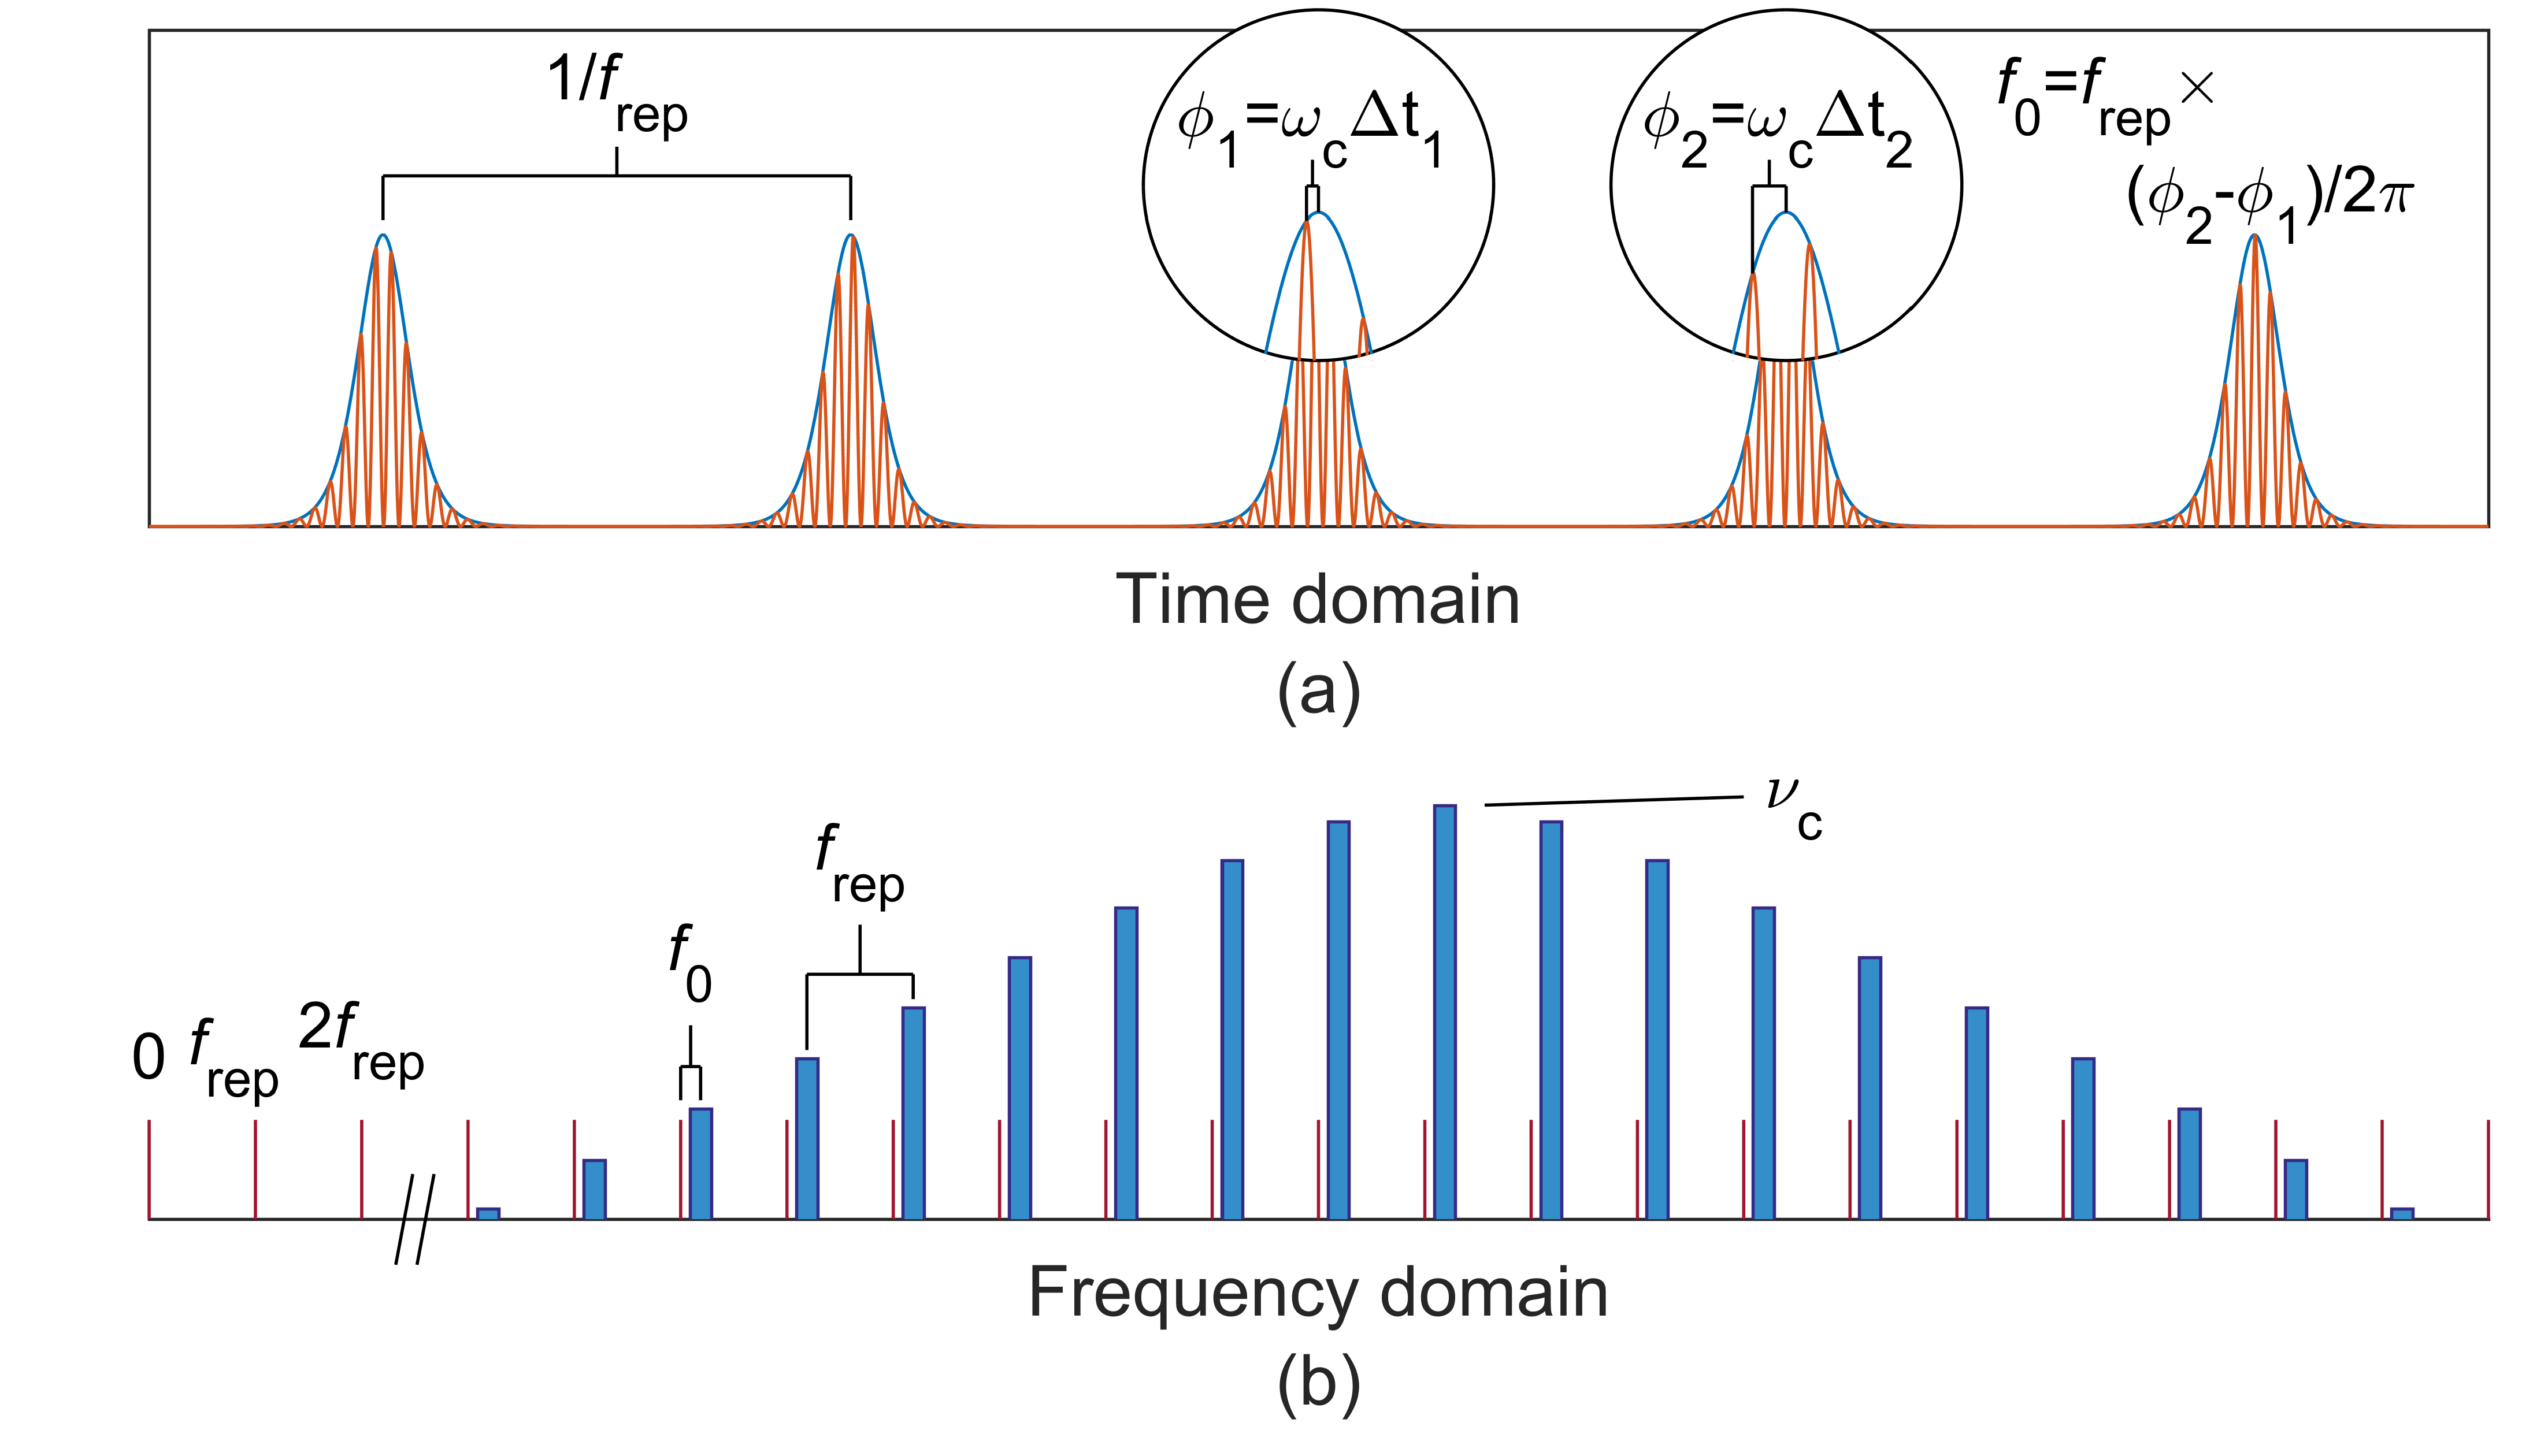
\includegraphics{\FigPath/Figures/Introduction/IntroFCbasics.png}
	\end{center}
	\caption[Optical frequency combs in the time and frequency domains]{\textbf{Optical frequency combs in the time and frequency domains.} (a) Time-domain depiction of a frequency comb as a train of pulses spaced by $1/f_{rep}$. The intensity envelope is shown in blue, and the carrier wave is shown in orange. The carrier-envelope offset frequency $f_0$ arises from a phase-slip of the carrier with respect to the intensity envelope from pulse to pulse. Specifically, if phases $\phi_j=\omega_c\Delta t_j$ are traced out by the carrier wave between its maximum and the $j$\textsuperscript{th} peak of the pulse train, then $f_0=\frac{\phi_{j+1}-\phi_j}{2\pi}f_{rep}$. (b) Frequency-domain depiction of the same frequency comb. The comb modes (shown in blue) are centered around an optical frequency $\nu_c$ and offset from harmonics of the repetition rate $f_{rep}$ (shown in red) by a frequency shift $f_0$. Note that the x-axis has been broken, and the zero-referenced mode numbers of the comb modes shown are large, e.g. $n\sim19340$ for a 10 GHz repetition-rate comb centered at 1550 nm wavelength (see Chapter \ref{chap:EOMCombs}). }
	\label{fig:CombBasics}
\end{figure} 



It is useful to consider a mathematical treatment of an optical pulse train to understand the relationships presented above. In the time domain, the electric field $E(t)$ of the pulse train consists of optical pulses that arrive periodically and have baseband (centered at zero frequency) field envelope $A(t)$ multiplying the carrier wave of angular frequency $\omega_c=2\pi\nu_c$:
\begin{equation}
E(t)=\sum_{k=-\infty}^{\infty} A(t-kT)e^{i\omega_c t}. \label{eq:pulsetrain}
\end{equation}
Here, $T$ is the repetition period of the pulse train. Eq. \ref{eq:pulsetrain} can be viewed as describing a laser of angular frequency $\omega_c$ with a time-varying amplitude. This temporal modulation leads to the distribution of the power across a spectrum whose width scales inversely with the temporal duration of $A$. Intuitively, the spectrum of the comb is the spectrum of the periodic baseband field envelope\footnote{which, as the spectrum of a periodic function, is already a comb.} $\Sigma_k A(t-kT)$, shifted in frequency by the multiplication with $e^{i\omega_c t}$ so that it is centered around the optical carrier. More formally, we can calculate the frequency content of the comb by calculating
\begin{equation}
\mathcal{F}\left\{E\right\}(\omega)\sim\left(\sum_{k=-\infty}^{\infty}\mathcal{F}\left\{A(t-kT)\right\}\right)*\delta(\omega-\omega_c).
\end{equation}
Here $\mathcal{F}$ denotes Fourier transformation and $*$ denotes convolution; this expression results from the Fourier transform's property that the transform of a product is the convolution of the transforms: $\mathcal{F}(A\cdot B)=\mathcal{F}(A)*\mathcal{F}(B)$. Now we use the Fourier transform's property that a temporal translation results in a linear spectral phase shift to obtain:
\begin{equation}
\mathcal{F}\left\{E\right\}\sim\left(\mathcal{F}\left\{A\right\}\times\sum_{k=-\infty}^{\infty}e^{-i\omega kT}\right)*\delta(\omega-\omega_c).
\end{equation}
The quantity $\Sigma_ke^{-i\omega kT}$ is the Fourier-series representation of the series of $\delta$-functions \mbox{$\Sigma_\mu\delta(\omega-2\pi\mu/T)$} (the \textit{Dirac comb}), so we have
\begin{equation}
\mathcal{F}\left\{E\right\}(\omega)\sim\left(\mathcal{F}\left\{A\right\}\times\sum_{\mu=-\infty}^{\infty}\delta\left(\omega-2\pi \mu/T\right)\right)*\delta(\omega-\omega_c),
\end{equation}
and performing the convolution leads to the replacement of $\omega$ with $\omega-\omega_c$, leading to:
\begin{equation}
\mathcal{F}\left\{E\right\}\sim\sum_{\mu=-\infty}^{\infty}\delta\left(\omega-\omega_c-\mu\omega_r\right)\mathcal{F}\left\{A\right\}(\omega-\omega_c), \label{eq:combspectrum}
\end{equation}
where $\omega_{rep}=2\pi f_{rep}=2\pi/T$. This expression indicates that the spectrum of the comb has frequency content at modes $\nu_\mu=\nu_c+\mu f_{rep}$, and that their amplitudes are determined by the spectrum of the baseband field envelope, shifted up to the optical carrier frequency $\nu_c$. This is the natural formulation in the case of a comb derived from a CW laser, but it obscures the carrier-envelope offset frequency in the difference between $\nu_c$ and the nearest multiple of the repetition rate, as discussed above. In practice, if $f_{rep}$ is known, then a measurement of $f_0$ is equivalent to a measurement of the frequency of the input CW laser.


\subsection{Frequency stabilization of optical pulse trains}

The scientific need for a method to measure optical frequencies motivated the development of optical frequency combs. While the measurement bandwidth of electronic frequency counters has improved since 1999, it remains limited to frequencies roughly \textit{ten thousand} times lower than the frequency of, e.g., visible red light. Frequency combs present a method for measurement of the unknown frequency $f_{opt}$ of an optical signal through heterodyne with a frequency comb---if $f_{opt}$ falls within the bandwidth of the frequency comb, then the frequency of the heterodyne between the comb and the signal is guaranteed to be less than $f_{rep}/2$. If the frequencies of the comb are known, measurement of the heterodyne with the signal reveals its frequency  $f_{opt}$, provided that the comb mode number and sign of the beat can be determined. This can be done via a wavelength measurement if sufficient precision is available, or by measuring the change $\partial f_b/\partial f_{rep}$, where $f_b$ is the measured frequency of the beat.

The utility of the optical frequency comb lies in the fact that measurement of the two frequencies $f_{rep}$ and $f_0$ is sufficient to determine the optical frequencies of all of the modes of the comb, thereby enabling frequency measurement of optical signals. Measurement of the repetition rates of optical pulse trains was possible before the realization of optical frequency comb technology, as this can be done by simply impinging the pulse train on a photodetector. Some pulse trains generated in new platforms have repetition rates too high for direct measurement in this way, but this challenge can be addressed by e.g. spectrally interleaving a lower repetition-rate comb \cite{Spencer2018,Briles2017}. In general, measurement of $f_0$ presents the more difficult challenge. It was the confluence of several technological developments around the turn of the twenty-first century that allowed detection and measurement of this frequency, thereby enabling creation of fully-stabilized modelocked-laser pulse trains: optical frequency combs.

The carrier-envelope offset frequency of a pulse train is challenging to measure because it describes evolution of the optical carrier wave underneath the intensity envelope, and therefore cannot be measured through straightforward detection of the intensity of the pulse train. Presently, the most straightforward way to measure $f_0$ is $f-2f$ \textit{self-referencing}. This can be performed only with a pulse train whose spectrum spans an octave---a factor of two in frequency. Given such an octave-spanning supercontinuum spectrum, a group of modes near mode number $N$ is frequency-doubled in a medium with the $\chi^{(2)}$ nonlinearity \cite{Boyd2003}. This frequency-doubled light is heterodyned with the native light in the supercontinuum with mode number near $2N$. The frequency of the resulting beat $f_b$ is:
\begin{align}
f_b&=f_{doubled}-f_{native}\\
&=2(Nf_{rep}+f_0)-(2Nf_{rep}+f_0)\\
&=f_0.
\end{align}
Such a scheme is implemented in an $f-2f$ \textit{interferometer}, which is depicted in Fig. \ref{fig:f2f}. Generating the necessary octave-spanning supercontinuum spectrum typically requires nonlinear spectral broadening of the pulse train after its initial generation except for in specific, carefully engineered cases (e.g. \cite{Briles2017,Fortier2003}). Achieving the required degree of spectral broadening while preserving the coherence properties of the pulse train is a significant challenge---in the past this has typically required launching a train of high energy ($\sim$1 nJ), temporally short ($\leq$ 100 fs) pulses into the spectral-broadening stage. Recent developments in nonlinear fiber and waveguide technology have relaxed these requirements slightly (e.g. Ref. \cite{Carlson2017}, also Chapter \ref{chap:EOMCombs}), but maintaining the coherence of the pulse train during spectral broadening remains an important consideration in designing optical frequency comb systems. 

The application of $f-2f$ self-referencing for full frequency-comb stabilization is discussed in Chapters \ref{chap:EOMCombs} and \ref{chap:PulsePicking}. Self-referencing of microresonator-based frequency combs is not a result presented explicitly in this thesis, but it is nonetheless a key step in the preparation of microcombs for applications and is a  motivation for the investigations into microcomb nonlinear dynamics that are presented in Chapters \ref{chap:PMPumping}-\ref{chap:FPLLE}.


\begin{figure}[htpb]
	\begin{center}
		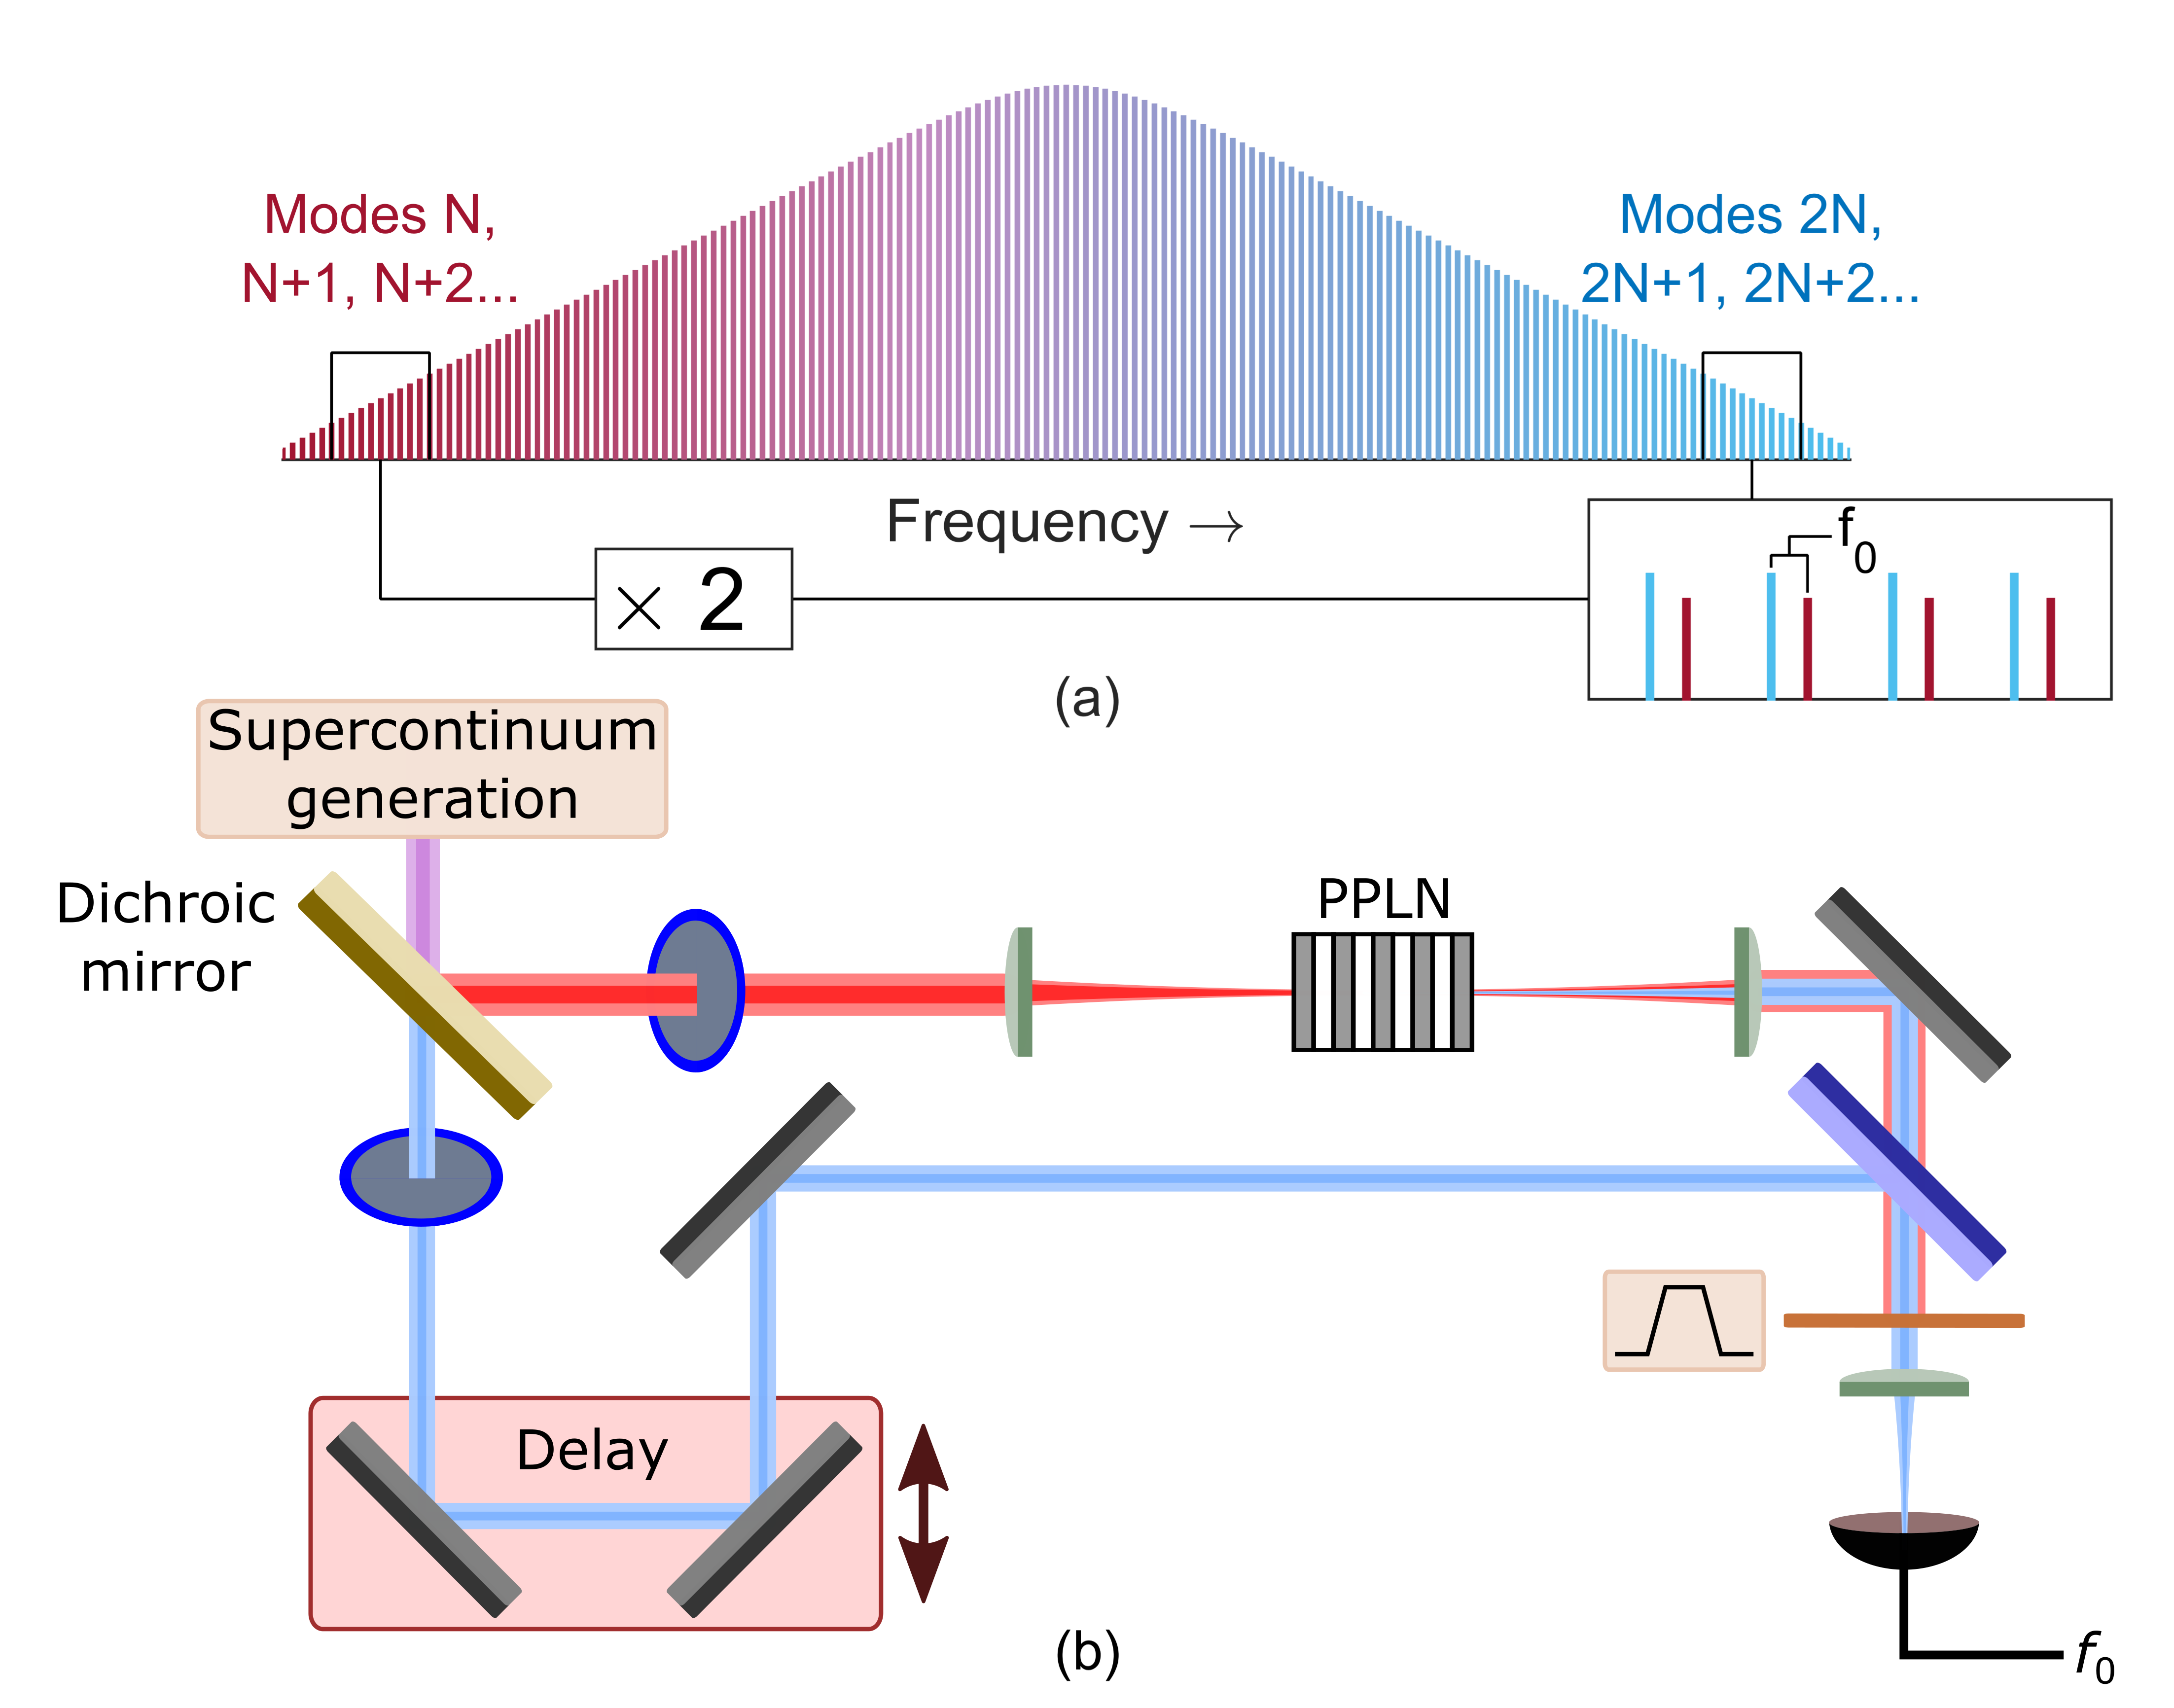
\includegraphics{\FigPath/Figures/Introduction/Introf2fv4.png}
	\end{center}
	\caption[Measurement of the carrier-envelope offset frequency via $f-2f$ self-referencing]{\textbf{Measurement of the carrier-envelope offset frequency $f_0$ via $f-2f$ self-referencing.} (a) Frequency-domain depiction of $f-2f$ self-referencing: Light on the low frequency end of an octave-spanning supercontinuum is frequency-doubled, and then heterodyned with light on the high frequency end near twice its frequency, enabling measurement of the carrier-envelope offset frequency. (b) Schematic depiction of an $f-2f$ interferometer: After supercontinuum generation, a dichroic mirror splits the light by wavelength, and the low-frequency end of the supercontinuum (red) is sent through a nonlinear crystal for frequency-doubling. Here the crystal is periodically-poled lithium niobate (PPLN), where quasi-phasematching is employed for efficient doubling of the target modes \cite{Hum2007}. The high-frequency end (blue) is sent through a delay stage, which can be adjusted to compensate for temporal walk-off between the spectral components (modes $\sim N$ and modes $\sim 2N$) required for self-referencing during the supercontinuum generation process. The two beams are then recombined by a beamsplitter and sent through a narrow optical band-pass filter centered around the doubled modes, which filters out light not necessary for $f_0$ measurement to increase the signal-to-noise ratio of the detection. Photodetection of the band-passed beam then reveals $f_0$. Waveplates in each path are used to optimize the polarization of the long-wavelength light for frequency-doubling and to ensure co-polarization of the two beams on the detector. }
	\label{fig:f2f}
\end{figure} 
 
%\chapter{Introduction to microresonator-based frequency combs}
 \label{chap:microresonators}

 
 This chapter introduces the basic physics of optical frequency-comb generation in Kerr-nonlinear microring resonators, with a particular emphasis on providing context for the results described in the subsequent chapters. This field emerged in 2007 with the first report of comb generation in silica microtoroids \cite{DelHaye2007}, and has evolved rapidly. There are facets to the field that are not discussed here; we note that a number of papers that review this topic have been published, each of which provides a unique perspective \cite{Kippenberg2011,Savchenkov2016,Chembo2016a,Pasquazi2018}. The combs generated in Kerr-nonlinear ring resonators, excluding those generated in definitively `macro' fiber loops, have generally been called microcombs, despite the fact that some of the resonators used to generate them have dimensions on the scale of several millimeters. Microcombs are an attractive technology because of their high repetition rates and small footprints, especially relative to modelocked-laser-based combs, which make them promising candidates for inclusion in integrated photonics systems. Microcomb generation has been reported in a variety of platforms, including the aforementioned silica microtoroids, silica wedge \cite{Lee2012,Yi2015} and rod \cite{DelHaye2013} resonators, crystalline magnesium-fluoride \cite{Liang2011} and calcium-fluoride \cite{Savchenkov2008} resonators, and silicon-nitride waveguide resonators \cite{Okawachi2011,Moss2013}, which have the advantage of being immediately amenable to photonic integration.
 
 For simplicity, and following the terminology of the field, we will refer to broadband optical spectra generated through frequency conversion in Kerr-nonlinear microring resonators as `Kerr combs,' even when the output is not strictly a coherent frequency comb. Finally, we note that although researchers have so far focused on Kerr-comb generation with the ring geometry, is also possible to generate Kerr combs in a Kerr-nonlinear Fabry-Perot (FP) cavity, as has been demonstrated in several experiments \cite{Braje2009,Obrzud2017}. Theoretical investigations of Kerr-comb generation with the FP geometry are presented in Chapter \ref{chap:FPLLE}.
 

 
 \section{Optical microring resonators} \label{sec:OMRR}
An optical microring resonator guides light for many round trips around a closed path in a dielectric medium by total internal reflection. The principle is the same as the guiding of light in an optical fiber, and indeed a `macroring' resonator can be constructed from a loop of fiber, using a fiber-optic coupler with a small coupling ratio as an input/output port. Microring resonators can be constructed by looping an optical waveguide back on itself, in which case the resonator provides index contrast and light confinement over a full 360\textsuperscript{o} of the modal cross-section. Alternatively, resonators can be realized with geometries that lack an inner radius dimension and therefore provide less spatial confinement. In this case they can host `whispering-gallery modes,'\footnote{In some sources the terminology `whispering-gallery mode resonator' has been applied more generally, but the analogy to the acoustic case seems most appropriate for resonators in which index contrast is not provided over a full 360\textsuperscript{o} of the modal cross-section. Otherwise it is unclear what makes a WGM resonator different from a fiber loop, which in the limit of large radius obviously does not host whispering-gallery modes. This issue of terminology is discussed in Ref. \citeNoBrackets{Ilchenko2006}.} so-called due to their similarity with the acoustic `whispering-gallery' waves that permit a listener on one side of St. Paul's cathedral (for example) to hear whispers uttered by a speaker on the other side of the cathedral. A schematic depiction of the basic components of a typical microring-resonator experiment is shown in Fig. \ref{fig:microringresonator}. Optical microring resonators have a host of characteristics that make them useful for photonics applications in general and for nonlinear optics in particular; these include the ease with which they can be integrated and the ability to tailor the spectral distribution of guided modes through careful resonator design, as well as the ultra-high quality factors that have been demonstrated ($\geq$ several hundred million). The resonator quality factor $Q$ is defined as $Q=\omega_0 \tau_{ph}=\nu_0/\Delta\nu$, where $\omega_0=2\pi\nu_0$ is the optical angular frequency, $\tau_{ph}$ is the photon lifetime, and $\Delta\nu$ is the resonance linewidth. The $Q$ can be interpreted literally as the optical phase that is traversed by the carrier wave during the photon lifetime and is a useful figure of merit for nonlinear optics.

\begin{figure}[htpb]
	\begin{center}
		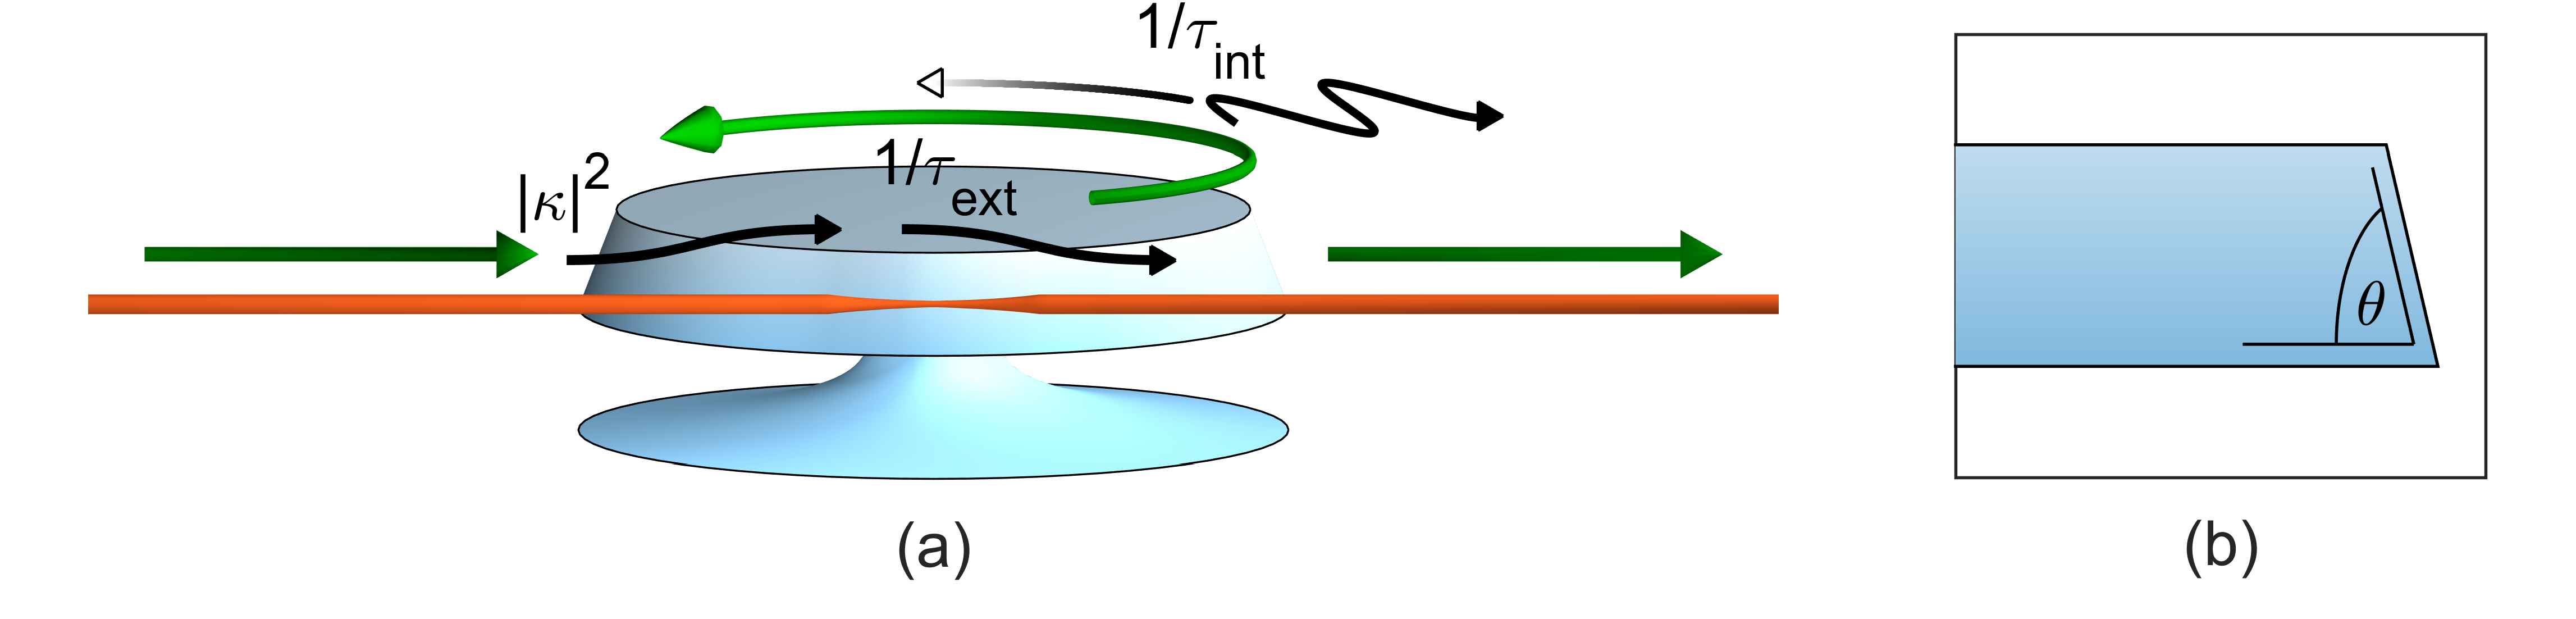
\includegraphics{\FigPath/Figures/Microresonators/MRmicroringresonatorv2.png}
	\end{center}
	\caption[Optical microdisk resonator]{\textbf{Optical microdisk resonator.} (a) An optical microring resonator with the disk geometry as described in Ref. \citeNoBrackets{Lee2012}, operated in a through-coupled configuration. Light (green) is evanescently coupled into and out of the resonator through a tapered optical fiber, shown in orange, which contacts the resonator near the fiber's point of smallest diameter. Light circulates in whispering-gallery modes concentric to the resonator's circumference. The black labels indicate the coupling and loss rates discussed in Sec. \ref{sec:resenhancement}: $|\kappa|^2$ is the rate at which incoming photons are coupled into the resonator, $1/\tau_{ext}$ is the rate at which circulating photons are coupling into the waveguide, and $1/\tau_{int}$ is the intrinsic loss rate. Here contributions to $1/\tau_{int}$ from absorption and radiative losses are depicted. (b) The wedge angle $\theta$ can be adjusted to control the geometric dispersion of the propagating whispering-gallery modes as described in Ref. \citeNoBrackets{Yang2016}, as $\theta$ dictates, for example, the extent to which larger (longer-wavelength) modes are confined further from the circumference of the wedge. }
	
	\label{fig:microringresonator}
\end{figure} 


A microring resonator supports propagating guided modes of electromagnetic radiation with (vacuum) wavelengths that evenly divide the optical round-trip path length: $\lambda_m=n_{eff}(\lambda_m)L/m$, with associated resonance frequencies $\nu_m=c/\lambda_m=mc/n_{eff}(\nu_m)L$. This leads to constructive interference from round trip to round trip. Here $m$ is the azimuthal mode number and the quantity $Ln_{eff}(\lambda_m)$ is the optical round-trip path length of the mode, where $n_{eff}(\lambda_m)$ defines an effective index of refraction related to the mode's propagation constant $k(\omega)$ via $k(\omega)=n_{eff}(\omega)\omega/c$ (see e.g. Refs. \cite{Agrawal2007,Calvo2007}; we use the symbol $k$ here and reserve the standard symbol $\beta$ for another quantity). The free-spectral range $f_{FSR}$ of a resonator is the \textit{local} frequency spacing between modes, calculated via:
\begin{align}
	f_{FSR}&\approx \frac{\nu_{m+1}-\nu_{m-1}}{2}\\
	&=\frac{\partial\nu_m}{\partial m}\\
	&=\frac{c}{n_{eff}(\nu)L}-\frac{mc}{n_{eff}^2(\nu)L}\frac{\partial n_{eff}}{\partial \nu}\frac{\partial \nu}{\partial m},
	\end{align}
	so that, rearranging, we obtain:
	\begin{equation}
	f_{FSR}=\frac{c/L}{\left(n_{eff}+\nu\frac{\partial n_{eff}}{\partial \nu}\right)}=\frac{c}{n_g L}=1/T_{RT},
\end{equation}
	where $n_g=n_{eff}+\nu\frac{\partial n_{eff}}{\partial \nu}$ is the group velocity of the mode and $T_{RT}$ is the mode's round-trip time. The effective index $n_{eff}$ is frequency dependent due to both intrinsic material dispersion and geometric dispersion, where the latter results for example from different sampling of material properties for different wavelength-dependent mode areas. A frequency-dependent $n_{eff}$ leads to a non-uniform spacing in the cavity modes in frequency despite the linearity of $\nu_m$ in $m$; equivalently this results in a frequency dependence of $n_g$ and $f_{FSR}$.
	
Depending on the design, microring resonators can support many transverse mode profiles, or just one. The former is typical of whispering-gallery-mode resonators that lack an inner radius, such as the wedge resonator shown in Fig. \ref{fig:microringresonator} or free-standing silica microrod resonators \cite{DelHaye2013}; the latter can be readily achieved using chip-integrated single-mode photonic waveguides. For a given resonator geometry, to calculate the frequency-dependent effective index $n_{eff}(\nu)$, thereby enabling calculation of the resonance frequencies and wavelengths, one must solve Maxwell's equations for the resonator geometry. Except in special cases of high symmetry (e.g. a dieletric sphere \cite{Oraevsky2002}), this is typically done numerically using finite-element modeling tools like COMSOL. The modes of an optical resonator, both within a mode family defined by a transverse mode profile (such that they differ only by azimuthal mode number $m$) and between mode families, must be orthogonal \cite{Haus1984}, with no linear coupling between them.

\subsection{Resonant enhancement in a microring resonator} \label{sec:resenhancement}
 The lifetime $\tau_{ph}$ of circulating photons in a resonator is fundamental to its fitness for applications. Generally, two processes lead to the loss of circulating photons: intrinsic dissipation that occurs at a rate $1/\tau_{int}$ and out-coupling to an external waveguide that occurs at a rate $1/\tau_{ext}$, leading to a total loss rate of $\tau_{ph}^{-1}=\tau_{ext}^{-1}+\tau_{int}^{-1}$. To understand the quantitative role of these parameters, we consider a cavity mode of frequency $\omega_0$ and described by instantaneous amplitude $a(t)$ (normalized such that $|a|^2=N$, the number of circulating photons) driven by a pump field with frequency $\wpl$ and rotating amplitude $s\propto\exp(i\wpl t)$ (normalized such that $|s|^2=S$, the rate at which photons in the coupling waveguide pass the coupling port) that is in-coupled with strength $\kappa$. The equation of motion for such a system is \cite{Haus1984}:
 \begin{equation}
 \frac{d a}{d t}=i\omega_0 a-\left(\frac{1}{2\tau_{int}}+\frac{1}{2\tau_{ext}}\right)a+\kappa s, \label{eq:coupledmotion}
 \end{equation}
 and the rates that determine the evolution of $a$ are shown schematically in Fig. \ref{fig:microringresonator}. We can immediately solve this equation by assuming that $a\propto\exp(i\wpl t)$, and we obtain:
 \begin{equation}
 a=\frac{\kappa s}{\left(\frac{1}{2\tau_{int}}+\frac{1}{2\tau_{ext}}\right)+i(\wpl-\omega_0)}. \label{eq:coupledsoln}
 \end{equation}
 
The coupling strength $\kappa$ into the waveguide and the out-coupling rate $1/\tau_{ext}$ are related by $|\kappa|^2=1/\tau_{ext}$; one can arrive at this conclusion by considering the special case $1/\tau_{int}=0$ and exploiting the time-reversal symmetry of the system under this condition \cite{Haus1984}. By squaring Eq. \ref{eq:coupledsoln} and inserting this relationship between $\kappa$ and $\tau_{ext}$, we find:
% 
% To extract anything further from this equation, we must derive a relationship between $\tau_{ext}$ and $\kappa$, which so far are not related. To do this, we exploit the time-reversal symmetry that is inherent in this system when there is no dissipation, that is, when $1/\tau_{int}=0$. In the case of only an initial excitation $N_0$ decaying into the waveguide with the driving term $s$ set to zero, we have $N=N_0e^{-t/\tau_{ext}}$. In this case, energy conservation guarantees that the rate $S_{out}$ at which photons propagate away from the resonator in the waveguide is $S_{out}=-dN/dt=N_0e^{-t/\tau_{ext}}/\tau_{ext}$; we therefore have $S_{out}=N/\tau_{ext}$. In the time-reversed system with $t\rightarrow-t$, this amplitude $S_{out}$ describes the rate of pumping: the cavity is resonantly driven with increasing power $S=S_{out}(-t)=N_0e^{t/\tau_{ext}}/\tau_{ext}$. In this case the frequency of the driving field $s$ can be written $\omega_0-i/2\tau_{ext}$. Inserting this frequency into Eq. \ref{eq:coupledsoln} gives the equations
% \begin{equation}
%  a=\kappa s \tau_{ext}
%  \end{equation}
%  and
%  \begin{equation}
%   N=|\kappa|^2 S \tau_{ext}^2.
%   \end{equation}
%   By comparing the relationships between $S_{out}$ and $N$ for the forward-evolving system and $S$ and $N$ for the backward-evolving system, we arrive at the relationship $|\kappa|^2=1/\tau_{ext}$. We can return to the case including dissipation and insert this expression for $\kappa$ into Eq. \ref{eq:coupledsoln}, which can then be squared to obtain:
   \begin{equation}
   N=\frac{\Delta\omega_{ext}S}{\Delta\omega^2/4+(\wpl-\omega_0)^2}, \label{eq:resenhancement}
   \end{equation}
   where we have defined the rates $\Delta\omega_{ext}=1/\tau_{ext}$, $\Delta\omega_{int}=1/\tau_{int}$, and $\Delta\omega=\Delta\omega_{ext}+\Delta\omega_{int}$. Two important observations can be drawn from Eq. \ref{eq:resenhancement}: First, the cavity response is Lorentzian with a full-width at half-maximum (FWHM) linewidth that is related to the photon lifetime via $\tau_{ph}=1/\Delta\omega$, and second, on resonance the number of circulating photons is related to the input rate by the factor $\Delta\omega_{ext}/\Delta\omega^2\ll1$. This factor is not yet the resonant enhancement, which we now calculate by considering the circulating power $P=N\hbar\omega_p/T_{RT}$ on resonance (when $\omega_p=\omega_0$):
   \begin{align}
   P=&\frac{4\Delta\omega_{ext}P_{in}/T_{RT}}{\Delta\omega^2}\\
   =&\frac{2 }{\pi}P_{in}\eta\mathcal{F},
   \end{align}
   where $\mathcal{F}=2\pi\tau_{ph}/T_{RT}=f_{FSR}/\Delta\nu$ is the resonator finesse, $\eta=\Delta\omega_{ext}/\Delta\omega$ is the coupling ratio, typically of order $\sim\frac{1}{2}$, and $P_{in}=\hbar\omega_p S$ is the power in the waveguide. Thus, the circulating power is approximately a factor $\mathcal{F}$ greater than the input power. The combination of this resonant enhancement and a small cavity mode volume enables very large circulating optical intensities in high finesse resonators, which is important for the application of microresonators in nonlinear optics. 


\subsection{Thermal effects in microresonators} \label{sec:thermaleffects}

%In a typical microresonator frequency-comb experiment, a frequency-tunable pump laser is coupled evanescently into and out of the resonator using a tapered optical fiber (for e.g. free-standing silica disc resonators) or a bus waveguide (for chip-integrated resonators, e.g. in silicon nitride rings). This thesis describes experiments in which the wavelength of the pump laser is always in the telecommunications band, near $\lambda=$1550 nm. However, other pump wavelengths are possible, and frequency combs have been generated with pumps ranging from the visible \cite{visiblecombs} to the outer reaches of the near infrared \cite{midIRcombs}\todo{true?}. When overlap between the evanescent mode of the fiber and a whispering-gallery mode of the resonator is achieved, with the frequency of the pump laser close to the resonant frequency of that mode, light will build up in the resonator and the transmission of the pump laser past the resonator will decrease.

In a typical microresonator frequency-comb experiment, a frequency-tunable pump laser is coupled evanescently into and out of the resonator using a tapered optical fiber \cite{Knight1997,Spillane2003} (for e.g. free-standing silica disc resonators) or a bus waveguide (for chip-integrated resonators, e.g. in silicon nitride rings). When spatial overlap and phase-matching ($n_{eff,res}\sim n_{eff,coupler}$ \cite{ShahHosseini2010}) between the evanescent mode of the coupler and a whispering-gallery mode of the resonator is achieved, with the frequency of the pump laser close to the resonant frequency of that mode, light will build up in the resonator and the transmission of the pump laser past the resonator will decrease.

In any experiment in which a significant amount of pump light is coupled into a resonator, one immediately observes that the cavity resonance lineshape in a scan of the pump-laser frequency is not Lorentzian as expected from Eq. \ref{eq:resenhancement}; plots of measured resonance lineshapes are shown in Fig. \ref{fig:MRthermal}a. This is because the resonator heats as it absorbs circulating optical power. Associated with this change in temperature are changes in the mode volume and the refractive index, described respectively by the coefficient of thermal expansion $\partial V/\partial T$ and the thermo-optic coefficient $\partial n/\partial T$. For typical microresonator materials the thermo-optic effect dominates, and $\partial n/\partial T>0$ leads to a decrease in the resonance frequency with increased circulating power in thermal steady state. Thus, for an adiabatic scan across the cavity resonance with decreasing laser frequency, as the laser approaches the resonance in frequency space and power is coupled into the resonator, the resonance frequency will begin to shift with the laser frequency, and a sawtooth-shaped resonance emerges.

%Since the volume of a pumped mode and the physical volume of the microresonator are both small, thermal effects have significant practical implications in microresonator experiments. As the volume of the mode heats (over a `fast thermal timescale') and this energy is conducted to and heats the rest of the resonator (over the `slow thermal timescale') \cite{Ilchenko1992},

%thermal bistability exists over a range of pump-laser frequencies $\wpl$. In particular, 

The thermal dynamics related to $\partial n/\partial T$ and $\partial V/\partial T$ dictate the signs and values of detuning $\omega_0-\omega_p$ that are readily accessible in experiment. Specifically, a calculation of the thermal dynamics of the system composed of the pump laser and the resonator reveals that when the pump laser with frequency $\omega_p$ is near the `cold-cavity' resonance frequency of a given cavity mode $\omega_{0,cold}$ the resonance has three possible thermally-shifted resonance frequencies $\omega_{0,shifted}$ at which thermal steady state is achieved \cite{Carmon2004}. Generally, these points are:
\begin{enumerate}
\item $\wpl>\omega_{0,shifted}$, blue detuning\footnote{Here we use the convention that the `color' of the detuning specifies the position of the laser with respect to the resonance---`blue' detuning means that the laser is more blue, or higher in frequency.} with significant coupled power and thermal shift
\item $\wpl<\omega_{0,shifted}$, red detuning with significant coupled power and thermal shift
\item $\wpl\ll\omega_{0}$, red detuning with insignificant coupled power and insigificant thermal shift
\end{enumerate}
These points are depicted schematically in Fig. \ref{fig:MRthermal}b. Steady-state point (1) is experimentally important, because in the presence of pump-laser frequency and power fluctuations it leads to so-called thermal `self-locking.' Specifically for steady-state point (1), this can be seen as follows: 
\begin{itemize}
	\item If the pump-laser power increases, the cavity heats, the resonance frequency decreases, the detuning increases, and the change in coupled power is minimized.
	\item If the pump-laser power decreases, the cavity cools, the resonance frequency increases, the detuning decreases, and the change in coupled power is minimized.
	\item If the pump-laser frequency increases, the cavity cools, the resonance frequency increases, and the change in coupled power is minimized.
	\item If the pump-laser frequency decreases, the cavity heats, the resonance frequency decreases, and the change in coupled power is minimized.
	\end{itemize}
This is in contrast with steady-state point (2), where each of the four pump-laser fluctuations considered above generates a positive feedback loop, with the result that any fluctuation will push the system towards point (1) or point (3) and so point (2) is unstable. This preference of the system to occupy point (1) or point (3) over a range of pump-laser detuning is referred to as thermal bistability. As a result of this bistability, point (2) (i.e. red detuning with significant coupled power) cannot be observed in an experimental scan of the pump laser across the resonance in either direction. As explained above, when the pump-laser frequency is decreased the resonance takes on a broad sawtooth shape, while in an increasing-frequency scan the resonance takes on a narrow pseudo-Lorentzian profile whose exact shape depends on the scan parameters relative to the thermal timescale. A second consequence is that, in the absence of other stabilizing effects, operation at red detuning with significant coupled power in a microresonator experiment requires special efforts to mitigate the effects of thermal instability.

%One consequence of this bistability is that the transmission profile of the pump laser takes on hysteretic behavior in a scan over a cavity resonance with significant pump power: in a decreasing frequency scan, the lineshape takes on a broad sawtooth shape, while in an increasing frequency scan,

%\begin{figure}[htpb]
%	\begin{center}
%		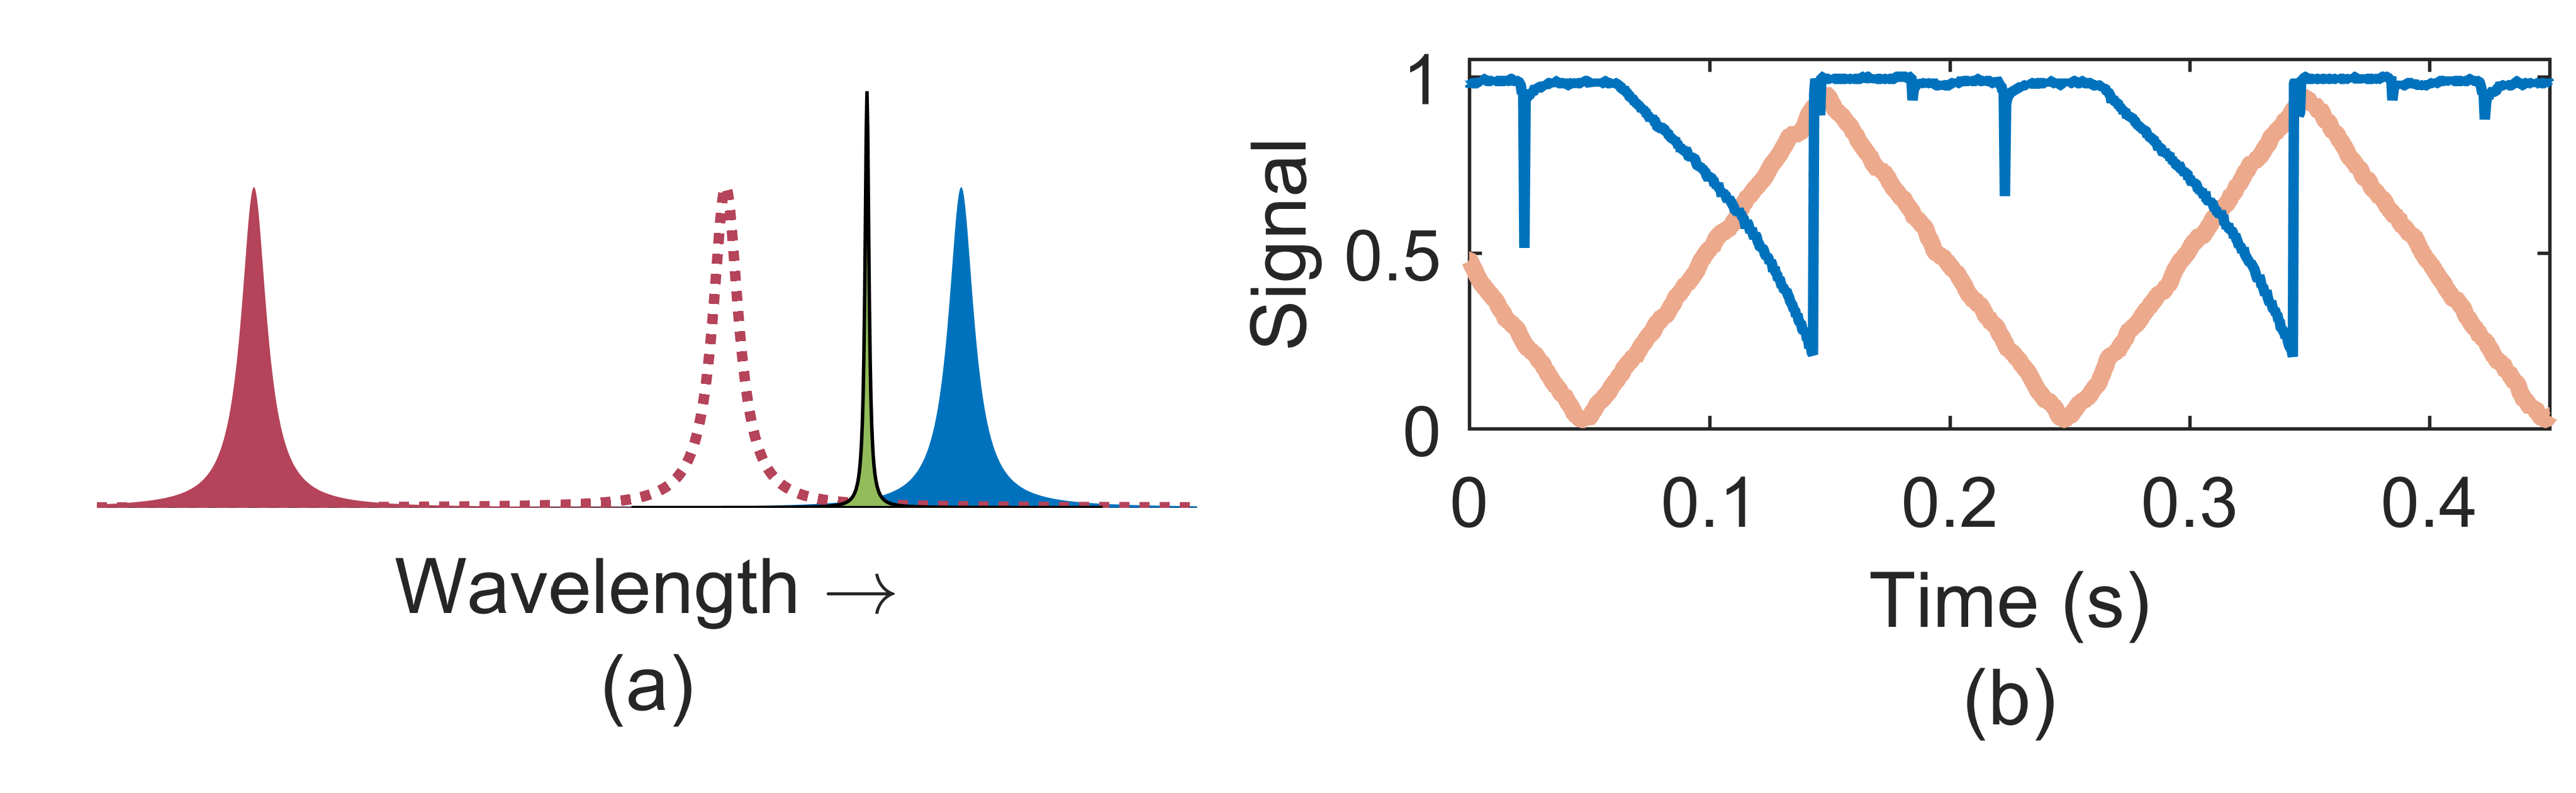
\includegraphics{\FigPath/Figures/Microresonators/MRthermal.png}
%	\end{center}
%	\caption[Thermal bistability in microresonators]{\textbf{Thermal bistability in microresonators.} (a) Depiction of the three steady-state points for the laser detuning. For fixed laser wavelength (green), stable steady-state points exist with relatively small blue detuning and significant coupled power (solid blue), and relatively large red detuning and little coupled power (solid red). An unstable steady-state point also exists with red detuning and significant coupled power (dashed red). Note in this terminology that the color of the detuning (red or blue) refers to the position of the laser relative to the position of the resonance in wavelength space. (b)~Measurement of power transmitted past the microresonator in an experiment using a $\sim$16.5 GHz-FSR microdisk resonator and a tapered fiber. The laser wavelength is adjusted by an intracavity piezo-electric crystal. Here, the control signal shown in orange corresponds to longer laser wavelength. As the laser wavelength is increased, the resonator heats and a sawtooth-shaped resonance is observed. As the resonator wavelength is decreased, the system will `flip' from steady-state point (3) to steady-state point (1), leading to observation of a narrow pseudo-Lorentzian resonance, with the exact shape depending on the thermal and scanning timescales.}
%	
%	\label{fig:MRthermal}
%\end{figure} 

\begin{figure}[htpb]
	\begin{center}
		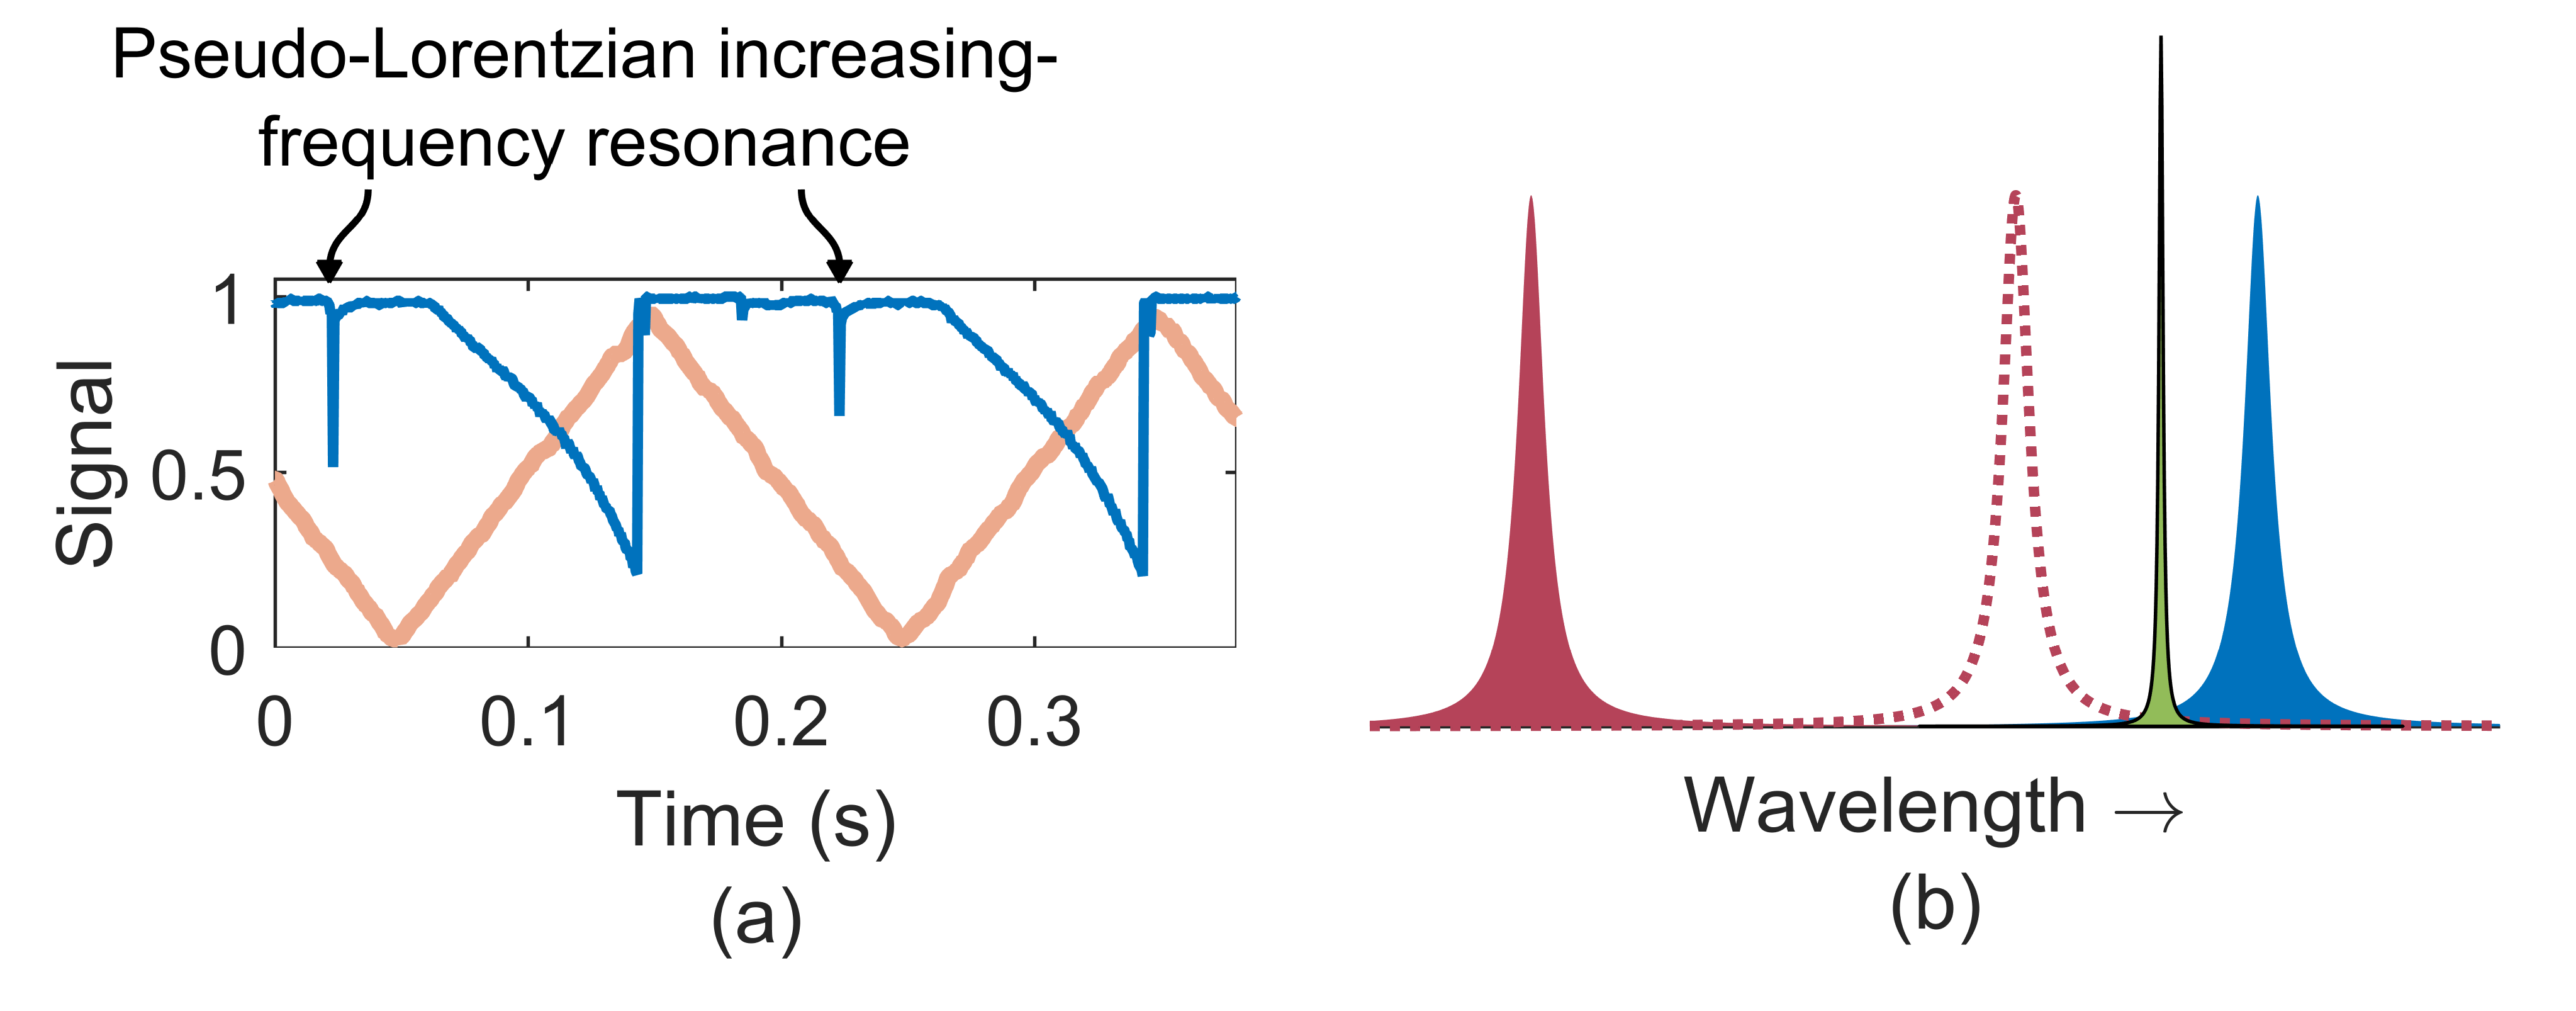
\includegraphics{\FigPath/Figures/Microresonators/MRthermalv4.png}
	\end{center}
	\caption[Thermal bistability in microresonators]{\textbf{Thermal bistability in microresonators.} (a)~Measurement of power transmitted past the microresonator (blue) in an experiment using a $\sim$16.5 GHz-FSR microdisk resonator and a tapered fiber. The wavelength of the pump laser is controlled by a piezo-electric crystal that adjusts the length of the laser cavity. Here, larger control signal (orange) corresponds to longer laser wavelength. As the laser wavelength is increased, the resonator heats and a sawtooth-shaped resonance is observed. Ultimately the resonator reaches a maximum temperature that depends on the pump power, and the laser then becomes red-detuned as the wavelength continues to increase; then the resonator rapidly cools and the resonance is lost. Shortly thereafter, the direction of the scan is reversed. As the resonator wavelength is decreased, the system will `flip' from steady-state point (3) to steady-state point (1), leading to observation of a narrow pseudo-Lorentzian resonance, with the exact shape depending on the thermal and scanning timescales. (b) Depiction of the three steady-state points for the laser detuning. For fixed laser wavelength (green), stable steady-state points exist with relatively small blue detuning and significant coupled power (solid blue), and relatively large red detuning and little coupled power (solid red). An unstable steady-state point also exists with red detuning and significant coupled power (dashed red). Note in this terminology that the color of the detuning (red or blue) refers to the position of the laser relative to the position of the resonance in wavelength space. }
	
	\label{fig:MRthermal}
\end{figure} 








\section{Microring resonator Kerr frequency combs}

The high circulating optical intensities accessible in resonators with long photon lifetimes find immediate application in the use of microresonators for nonlinear optics. The experiments described in this thesis are conducted in silica microresonators. Silica falls into a broader class of materials that exhibit both centro-symmetry, which dictates that the second-order nonlinear susceptibility $\chi^{(2)}$ must vanish, and a significant third-order susceptibility $\chi^{(3)}$. The $n$\textsuperscript{th}-order susceptibility is a term in the Taylor expansion describing the response of the medium's polarization to an external electric field \cite{Boyd2003}: $P=P_0+\epsilon_0 \chi^{(1)} E + \epsilon_0 \chi^{(2)} E^2 + \epsilon_0 \chi^{(3)} E^3+...$. The effect of $\chi^{(3)}$ can be described in a straightforward way as a dependence of the refractive index on the local intensity \cite{Agrawal2007},
\begin{equation}
n=n_0+n_2 I \label{eq:KerrIndex}
\end{equation}
where $n_2=\frac{3\chi^{(3)}}{4n_0^2\epsilon_0 c}$ is called the Kerr index \cite{DelCoso2004,Agrawal2007}. The intensity-dependence of the refractive index resulting from the third-order susceptibility $\chi^{(3)}$ is referred to as the optical Kerr effect and enables the self-phase modulation (SPM), cross-phase modulation (XPM), and four-wave mixing (FWM) nonlinear processes \cite{Boyd2003}. Four-wave mixing is a general frequency-domain description of an energy-conserving interaction between fields of up to four different frequencies, as depicted in Figs. \ref{fig:MRfwm}a and b; self-phase modulation and cross-phase modulation can be thought of as time-domain descriptions of particular cases of FWM. In SPM and XPM the nonlinear interaction leads to intensity-dependent phase shifts of the field. If the intensity varies in time, for example in the case of an optical pulse, then the resulting time-varying nonlinear phase shift applies a chirp to the pulse. This can lead to modification of the pulse's spectrum, including the generation of new frequency components.\footnote{SPM doesn't \textit{always} lead to the generation of new frequency components. For example, solitons can propagate without becoming chirped through a balance between SPM and dispersion, and SPM can even lead to narrowing of the bandwidth of a pulse when e.g. the chirp generated by SPM has sign opposite to an existing chirp on the pulse.}

%\footnote{This terminology is sometimes used rather loosely and it is useful to avoid being too dogmatic about the differences between SPM and FWM: for example, the process of a short optical pulse acquiring a chirp during propagation in a Kerr medium is sometimes attributed to self-phase modulation, but the acquisition of the chirp is explicitly dependent on the fact that the pulse is broadband.}


\begin{figure}[htpb]
	\begin{center}
		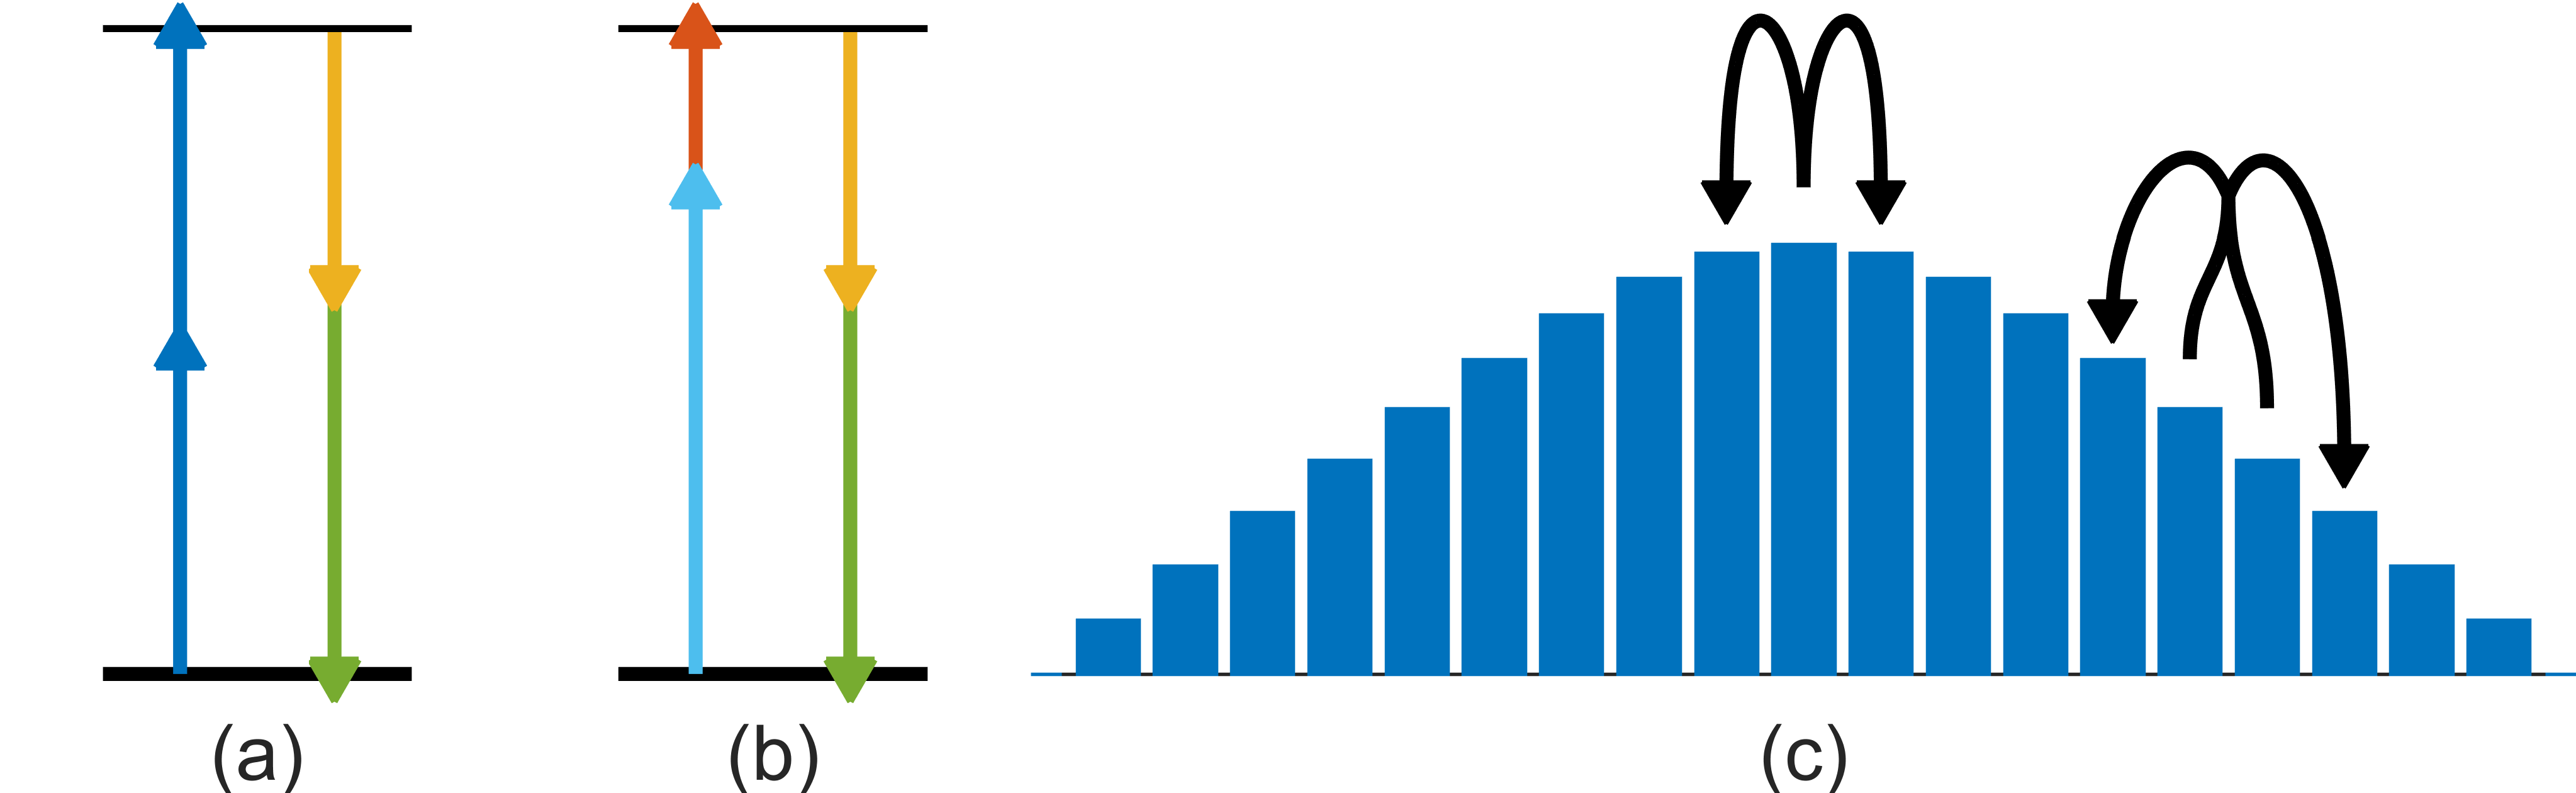
\includegraphics{\FigPath/Figures/Microresonators/MRfwm.png}
	\end{center}
	\caption[An illustration of four-wave mixing and frequency-comb generation.]{\textbf{An illustration of four-wave mixing and frequency-comb generation.} (a)~Degenerate four-wave mixing, in which two fields of the same frequency $\omega_1$ (blue) mix and generate fields at two new frequencies $\omega'$ and $\omega''$ (yellow and green). The schematic indicates the energy-conversation requirements of the process, which can be written as $2\omega_1=\omega'+\omega''$. (b) Non-degenerate four-wave mixing, in which two fields of different frequencies $\omega_2$ and $\omega_3$ (light blue and orange) mix to generate fields at frequencies $\omega'$ and $\omega''$ (yellow and green). Energy conservation is now expressed as $\omega_2+\omega_3=\omega'+\omega''$. (c) Schematic depiction of one degenerate FWM step and one non-degenerate FWM step in a cascaded four-wave mixing process that generates a frequency comb. \footnotesize{Figure after Ref. \citeNoBrackets{Kippenberg2011}.}}
	
	\label{fig:MRfwm}
\end{figure} 

For FWM to efficiently lead to the generation of new frequencies in some medium or waveguide it must be effectively phasematched, meaning that the quantity \cite{Stolen1982}
\begin{equation}
\Delta k=k(\omega_1)+k(\omega_2)-k(\omega')-k(\omega''),
\end{equation}
where $k(\omega)=n_{eff}(\omega)\omega/c$ is the propagation constant, should be made as small as possible; in the above the four frequencies correspond to those depicted in Figs. \ref{fig:MRfwm}a and b. In a ring resonator, FWM is intrinsically phasematched in interactions between fields propagating in modes with azimuthal mode numbers $m_1$, $m_2$, $m'$, and $m''$ such that $m_1+m_2=m'+m''$ \cite{Kippenberg2004}. Reports of few-mode parametric oscillation in microresonators based on FWM preceded the first observations of Kerr-comb generation \cite{Kippenberg2004, Savchenkov2004,Agha2007}.




%Measurements indicated that the frequency spacing was uniform to a precision of $7.3 \times 10^{-18}$, thereby establishing that the output of the system was a frequency comb.

In 2007, the remarkable observation by Del'Haye et al. of \textit{cascaded four-wave mixing} (CFWM, shown in Fig. \ref{fig:MRfwm}c) in anomalously-dispersive ($k''=\frac{\partial^2}{\partial\omega^2}\frac{n_{eff}(\omega)\omega}{c}<0$) toroidal silica microcavities on silicon chips brought about a new era for frequency comb research. They observed the generation many co-circulating optical fields that were uniformly spaced by $f_{rep}$ ranging from 375 GHz to $\sim$750 GHz (depending on the platform) \cite{DelHaye2007}. This result showed that the non-uniform distribution of cavity resonance frequencies due to dispersion could be overcome to generate an output with many equidistant frequency modes. A second important development occurred in 2012, when Herr et al. reported the generation of frequency combs corresponding in the time domain to single circulating optical `soliton' pulses \cite{Herr2014} (2012 pre-print \cite{Herr2012a}). This observation followed the observation of solitons in formally-equivalent passive fiber-ring resonators in 2010 \cite{Leo2010a}. Due to unique properties that make them particularly well-suited for applications, as discussed in Sec. \ref{sec:LLEsolitons}, the generation and manipulation of soliton combs has become a significant priority in microcomb research. 

\subsection{A model for Kerr-comb nonlinear optics: The Lugiato-Lefever equation}\label{sec:LLE}

Kerr-comb generation can be motivated and partially understood through the CFWM picture \cite{Herr2012}, but the phase and amplitude degrees of freedom for each comb line mean that CFWM gives rise to a rich space of comb phenomena---it is now known that Kerr combs can exhibit several fundamentally distinct outputs.  A useful model for understanding this rich space is the Lugiato-Lefever equation (LLE), which was shown to describe microcomb dynamics by Chembo and Menyuk \cite{Chembo2013} through Fourier-transformation of a set of coupled-mode equations describing CFWM and by Coen, Randle, Sylvestre, and Erkintalo \cite{Coen2013a} through time-averaging of a more formally-accurate model for a low-loss resonator (as first performed by Haelterman, Trillo, and Wabnitz \cite{Haelterman1992a}).  The LLE is a nonlinear partial-differential equation that describes evolution of the normalized cavity field envelope $\psi$ over a slow time $\tau=t/2\tau_{ph}$ in a frame parametrized by the ring's azimuthal angle $\theta$ (running from $-\pi$ to $\pi$) co-moving at the group velocity.\footnote{The co-moving azimuthal angle $\theta$ is analogous to the `fast time' variable that appears in, for example, the nonlinear Schrodinger equation for fiber-optic pulse propagation \cite{Agrawal2007}, and it can be transformed explicitly to a fast time $t$ via $t=T_{RT}\times\frac{\theta}{2\pi}$.} A derivation of the LLE is provided in Appendix \ref{app:LLEfromIkeda}. The equation in the notation of Chembo and Menyuk, as it will be used throughout this thesis, reads:
\begin{equation}
\frac{\partial \psi}{\partial \tau}=-(1+i \alpha) \psi + i|\psi|^2 \psi -i \frac{\beta_2}{2} \frac{\partial^2 \psi}{\partial \theta^2} +F. \label{eq:LLE}
\end{equation}

This equation describes $\psi$ over the domain $-\pi\leq\theta\leq+\pi$ with periodic boundary conditions $\psi(-\pi,\tau)=\psi(\pi,\tau)$. Here $F$ is the field strength of the pump laser, with $F$ and $\psi$ both normalized so that they  take the value 1 at the absolute threshold for parametric oscillation: $F=\sqrt{\frac{8 g_0\Delta\omega_{ext}}{\Delta\omega^3}\frac{P_{in}}{\hbar \wpl}}$, $|\psi|^2=\frac{2g_0T_{RT}}{\hbar\wpl\Delta\omega}P_{circ}(\theta,\tau)$, so that $|\psi(\theta,\tau)|^2$ is the instantaneous normalized power at the co-moving azimuthal angle $\theta$. Here $g_0=n_2 c \hbar \wpl^2/n_g^2 V_0$ is a parameter describing the four-wave mixing gain, $\Delta\omega_{ext}$ is the rate of coupling at the input/output port, $\Delta\omega=1/\tau_{ph}$ is the FWHM resonance linewidth, $P_{in}$ is the pump-laser power, $P_{circ}(\theta,\tau)$ is the local circulating power in the cavity, $\hbar$ is Planck's constant, and $\wpl$ is the pump-laser frequency. The parameters $n_2$, $n_g$, and $V_0$ describe the nonlinear (Kerr) index (see Eqn. \ref{eq:KerrIndex}), the group index of the mode, and the effective nonlinear mode volume at the pump frequency; $L$ is the physical round-trip length of the ring cavity. 

The parameters $\alpha$ and $\beta_2$ describe the frequency detuning of the pump laser and second-order dispersion of the resonator mode family into which the pump laser is coupled, both normalized to half the cavity linewidth: 
\begin{align}
\alpha&=-\frac{2(\wpl-\omega_0)}{\Delta\omega},\\
\beta_2&=-\frac{2 D_2}{\Delta\omega};
\end{align} here $D_2=\left.\frac{\partial^2\omega_\mu}{\partial \mu^2}\right|_{\mu=0}$ is the second-order modal dispersion parameter, where $\mu$ is the pump-referenced mode number of Eq. \ref{eq:combfreqsnew}. The parameters $D_1=\left.\frac{\partial\omega_\mu}{\partial\mu}\right|_{\mu=0}=2\pi f_{FSR}$ and $D_2$ are related to the derivatives of the propagation constant $k(\omega)=\frac{n_{eff}(\omega)\omega}{c}$ via $D_1=2\pi/Lk'$ and $D_2=-D_1^2\frac{k''}{k'}$. It is useful to note that $k'=1/v_g$, where $v_g$ is the group velocity in the medium, and $k''$ is often referred to as the GVD parameter and denoted by $\beta_2$, which here is reserved for the dispersion parameter in the LLE. Expressions for higher-order modal dispersion parameters $D_n$ in terms of the expansion of the propagation constant can be obtained by evaluating the equation $D_{n>1}=(D_1\frac{\partial}{\partial \omega})^{n-1} D_1$, and may be incorporated into the LLE up to desired order $N$ through the replacement:
\begin{equation}
-i\frac{\beta_2}{2}\frac{\partial^2\psi}{\partial\theta^2}\rightarrow +\sum_{n=1}^N i^{n+1} \frac{\beta_n}{n!}\frac{\partial^n\psi}{\partial\theta^n},
\end{equation}
where $\beta_n=-2D_n/\Delta\omega$. This thesis describes frequency-comb generation in anomalously-dispersive resonators, and so $\beta_2<0$ throughout.

The formulation of the LLE in terms of dimensionless normalized parameters helps to elucidate the fundamental properties of the system and facilitates comparison of results obtained in platforms with widely different experimental conditions. The LLE relates the time-evolution of the intracavity field (normalized to its threshold value for cascaded four-wave mixing) to the power of the pump laser (normalized to its value at the threshold for cascaded four-wave mixing), the pump-laser detuning (normalized to half the cavity linewidth), and the cavity second-order disperison quantified by the change in the FSR per mode (normalized to half the cavity linewidth). One example of the utility of this formulation is that it makes apparent the significance of the cavity linewidth in determining the output comb, and underscores the fact that optimization of the dispersion, for example, without paying heed to the effect of this optimization on the cavity linewidth, may not yield the desired results. This adds an additional layer of complexity to dispersion engineering relative to straight waveguides.

The LLE is, of course, a simplified description of the dynamics occurring in the microresonator. It abstracts the nonlinear dynamics and generally successfully describes the various outputs that can be generated in a microresonator frequency comb experiment. The LLE is a good description of these nonlinear dynamics when the resonator photon lifetime, mode overlap, and nonlinear index $n_2$ are roughly constant over the bandwidth of the generated comb, and when the dominant contribution to nonlinear dynamics is simply the self-phase modulation term $i|\psi|^2\psi$ arising from the Kerr nonlinearity. The LLE neglects the polarization of the electric field ($\psi$ is a scalar), as well as thermal effects and the Raman scattering and self-steepening nonlinearities, although in principle each of these can be included \cite{Hansson2018,Herr2014,Chembo2015,Agrawal2007}. It is also worth emphasizing that the LLE can be derived from a more formally-accurate Ikeda map (as explained by Coen et al. \cite{Coen2013a}), in which the effect of localized input- and output-coupling is included in the model. This derivation is accomplished by `delocalizing' the pump field and the output-coupling over the round trip, including only their averaged effects. This is an approximation that is valid in the limit of high finesse due to the fact that the cavity field cannot change on the timescale of a single round trip, but as a result the LLE necessarily neglects all dynamics that might have some periodicity at the round-trip time; the fundamental timescale of LLE dynamics is the photon lifetime. 




%The LLE provides a useful framework for the prediction of comb properties and the exploration of avenues for new research, but also has proven to be an important tool in the interpretation of Kerr-comb experimental results. A primary reason for this is the difficulty of directly characterizing the time-domain output of a microresonator---typically, available tools enable measurement of time-averaged optical spectra and measurement of the comb's output power within the bandwidth of the photodetectors (generally $\lesssim$ 50 GHz) and amplifiers used for the measurement. Since neither records phase information and the latter lacks response on the timescale of, e.g., temporal pulses with duration less than a microresonator's round-trip time, these measurements are insufficient to determine the time-domain output of the microresonator. By providing a mathematical formalism that restricts the possible behaviors of the intracavity field $\psi$, the LLE enables inference of the temporal intensity profile $|\psi(\theta,\tau)|^2$ from the spectrum $|\psi_\mu(\tau)|^2$, which is readily measured in experiment.  \todo{How does FROG fit into this discussion?}

\section{Description of Kerr-comb outputs using the Lugiato-Lefever equation}

The LLE provides a useful framework for the prediction and interpretation of experimental results. Basically, it predicts the existence of two fundamentally distinct types of Kerr-combs: extended temporal patterns and localized soliton pulses. These predictions are born out by experiments, the interpretation of which is facilitated by insight gained from the LLE. In the remainder of this chapter I briefly present some analytical results that can be obtained from the LLE about the behavior of the continuous-wave (CW) field that exists in the resonator in the absence of Kerr-comb formation, and then discuss these two types of comb outputs. This discussion provides context for the results presented in the next two chapters. Fig. \ref{fig:MRLLEspace} summarizes the results that will be presented in the remainder of this chapter, and in particular shows the values of the parameters $\alpha$ and $F^2$ at which solitons and extended patterns can be obtained.



\begin{figure}[htpb]
	\begin{center}
		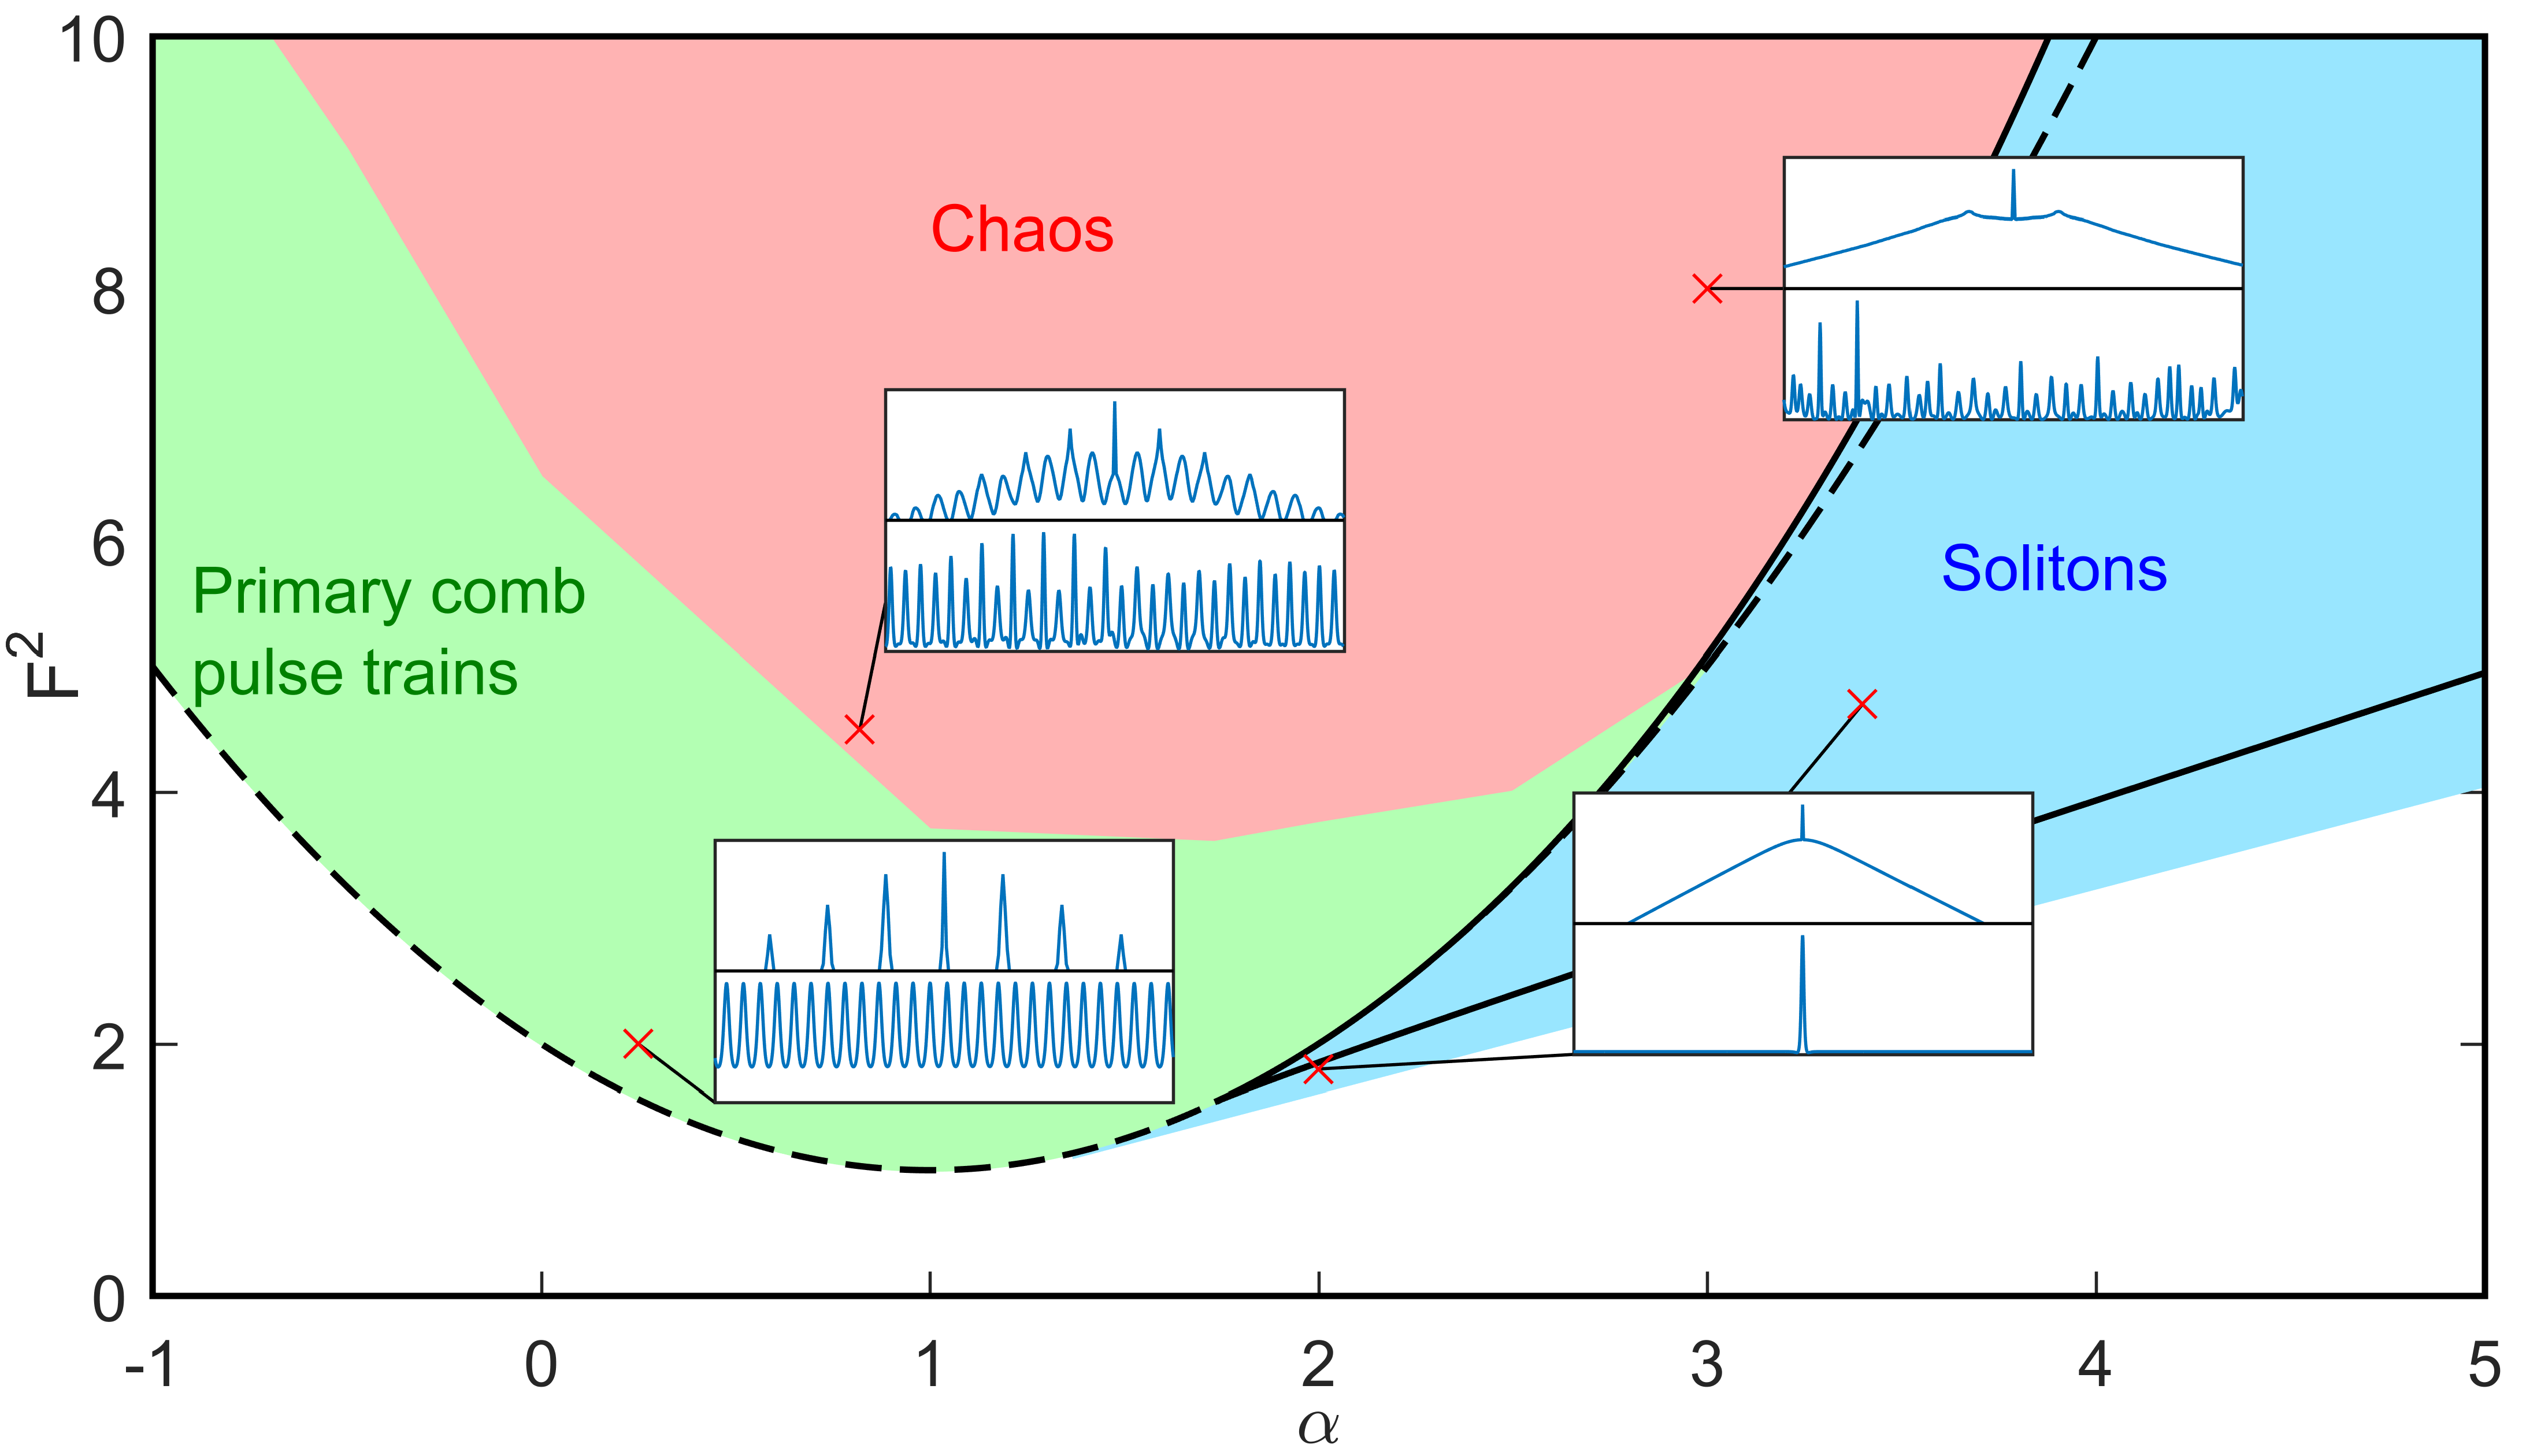
\includegraphics{\FigPath/Figures/Microresonators/MRLLEspace.png}
	\end{center}
	\caption[Solution space for the Lugiato-Lefever equation]{\textbf{Solution space for the Lugiato-Lefever equation.} Depiction of the various behaviors exhibited by $\psi$ as a function of its position in the $\alpha-F^2$ plane; this predicts the type of Kerr-comb output as a function of the pump-laser detuning and power, the parameters that are most readily adjusted in experiment. Curves plotted in black are obtained through analytical investigation of the LLE; these include the threshold curve for parametric oscillation (dashed black, Eq. \ref{eq:F2thresh}) and the lines obtained via $\rho(\alpha,F^2)=\rho_\pm(\alpha)$ (solid black, Eq. \ref{eq:rhopm}), which define the region where the LLE exhibits multiple flat solutions (i.e. solutions such that $\partial \psi/\partial \theta=0$, Eq. \ref{eq:LLEstat}). Extended patterns arise above the threshold curve through modulation instability. Solitons exist outside of the threshold curve at higher red detuning, up to an approximate maximum $\alpha_{max}=\pi^2 F^2/8$. The lines bounding the existence of chaos are not known precisely, and in fact chaos can be observed in simulation outside of the threshold curve at values $\alpha>\alpha_{thresh,+}$ (Eq. \ref{eq:alphathresh}). Insets show representative simulation results for the various types of comb outputs in the frequency (top) and time (bottom) domains. \footnotesize{Fig. after Ref. \citeNoBrackets{Godey2014}}.
	 }
	
	\label{fig:MRLLEspace}
\end{figure} 



%
%In the following subsections I introduce two fundamentally-distinct types of Kerr-combs. This provides important context for the results presented in the next two chapters. 

\subsection{Analytical investigation of the resonator's CW response}\label{sec:MRanalyticalcurves}
Some insight into comb dynamics can be obtained via analytical investigations of the LLE, Eq. \ref{eq:LLE}. This section largely follows the analysis of Ref. \citeNoBrackets{Godey2014}, with similar analysis having been performed elsewhere, for example in Refs. \cite{Coen2013a} and \cite{Barashenkov1996}. When the derivative term $\partial^2\psi/\partial\theta^2$ in the LLE is non-zero, $\psi$ is necessarily broadband, and a Kerr comb has been formed. There are no known exact analytical solutions to the LLE to describe Kerr-comb outputs, which must instead be numerically simulated (see Appendix \ref{app:numericalsims}). However, flat solutions $\psi_{CW}$ to the LLE  may be calculated by setting all derivatives to zero---when these solutions can be realized physically (discussed below), they describe a CW field in the resonator. Upon setting the derivatives in the LLE to zero, one finds:
\begin{equation}
F=(1+i\alpha)\psi_{CW}-i|\psi_{CW}|^2\psi_{CW}. \label{eq:LLEstat}
\end{equation}
The circulating intensity $\rho=|\psi_{CW}|^2$ is obtained by taking the modulus-square of Eq. \ref{eq:LLEstat} to obtain:
\begin{align}
F^2&=\left(1+(\alpha-\rho)^2\right)\rho\label{eq:LLEstat2},\\
&=\rho^3-2\alpha\rho^2+(\alpha^2+1)\rho,
\end{align} 
whereupon this equation can be numerically solved for $\rho$. As a third-order polynomial in $\rho$ this equation has three solutions, one or three of which may be real; the complex solutions are unphysical. The function $F^2(\alpha,\rho)$ defined by this equation uniquely determines $F^2$ given $\alpha$ and $\rho$. We now consider plotting a graph of $F^2(\alpha,\rho)$ with $\alpha$ held constant; examples are given in Fig. \ref{fig:MRcurves}. By noting that $F^2(\alpha,\rho=0)=0$ and $\left.\partial F^2/\partial \rho\right|_{\rho=0}>0$, we can conclude that a graph of $F^2(\alpha,\rho)$ will cross the same value $F^2$ three times if $F^2$ is between the extremal values $F^2_\pm(\alpha)$ at which $\partial F^2/\partial\rho=0$. This means that three real solutions $\rho_1$, $\rho_2$, and $\rho_3$ for the inverted function $\rho(\alpha,F^2)$ exist for each value of $F^2$ between $F^2_-(\alpha)$ and $F^2_+(\alpha)$. The values $F^2_\pm(\alpha)$ bounding  this region of degeneracy in $\rho$ are found by inserting the values $\rho_\pm$ at which $\partial F^2/\partial\rho=0$ into Eq. \ref{eq:LLEstat2}. That is, $F^2_\pm(\alpha)=F^2(\alpha,\rho_\mp)$, where:
\begin{equation}
\rho_\pm=\frac{2\alpha\pm\sqrt{\alpha^2-3}}{3}.\label{eq:rhopm}
\end{equation}
For pump powers outside of the interval $[F^2_-(\alpha),F^2_+(\alpha)]$, which varies with $\alpha$, there is only one real solution $\rho$; within this interval there are three. This is illustrated in Fig. \ref{fig:MRcurves}. The smallest value of $F^2$ at which the stationary curve $\rho$ becomes multivalued is found to be $F^2=8\sqrt{3}/9$ by solving for $\rho_-=\rho_+$ and inserting the corresponding values into Eq. \ref{eq:LLEstat2}.

\begin{figure}[htpb]
	\begin{center}
		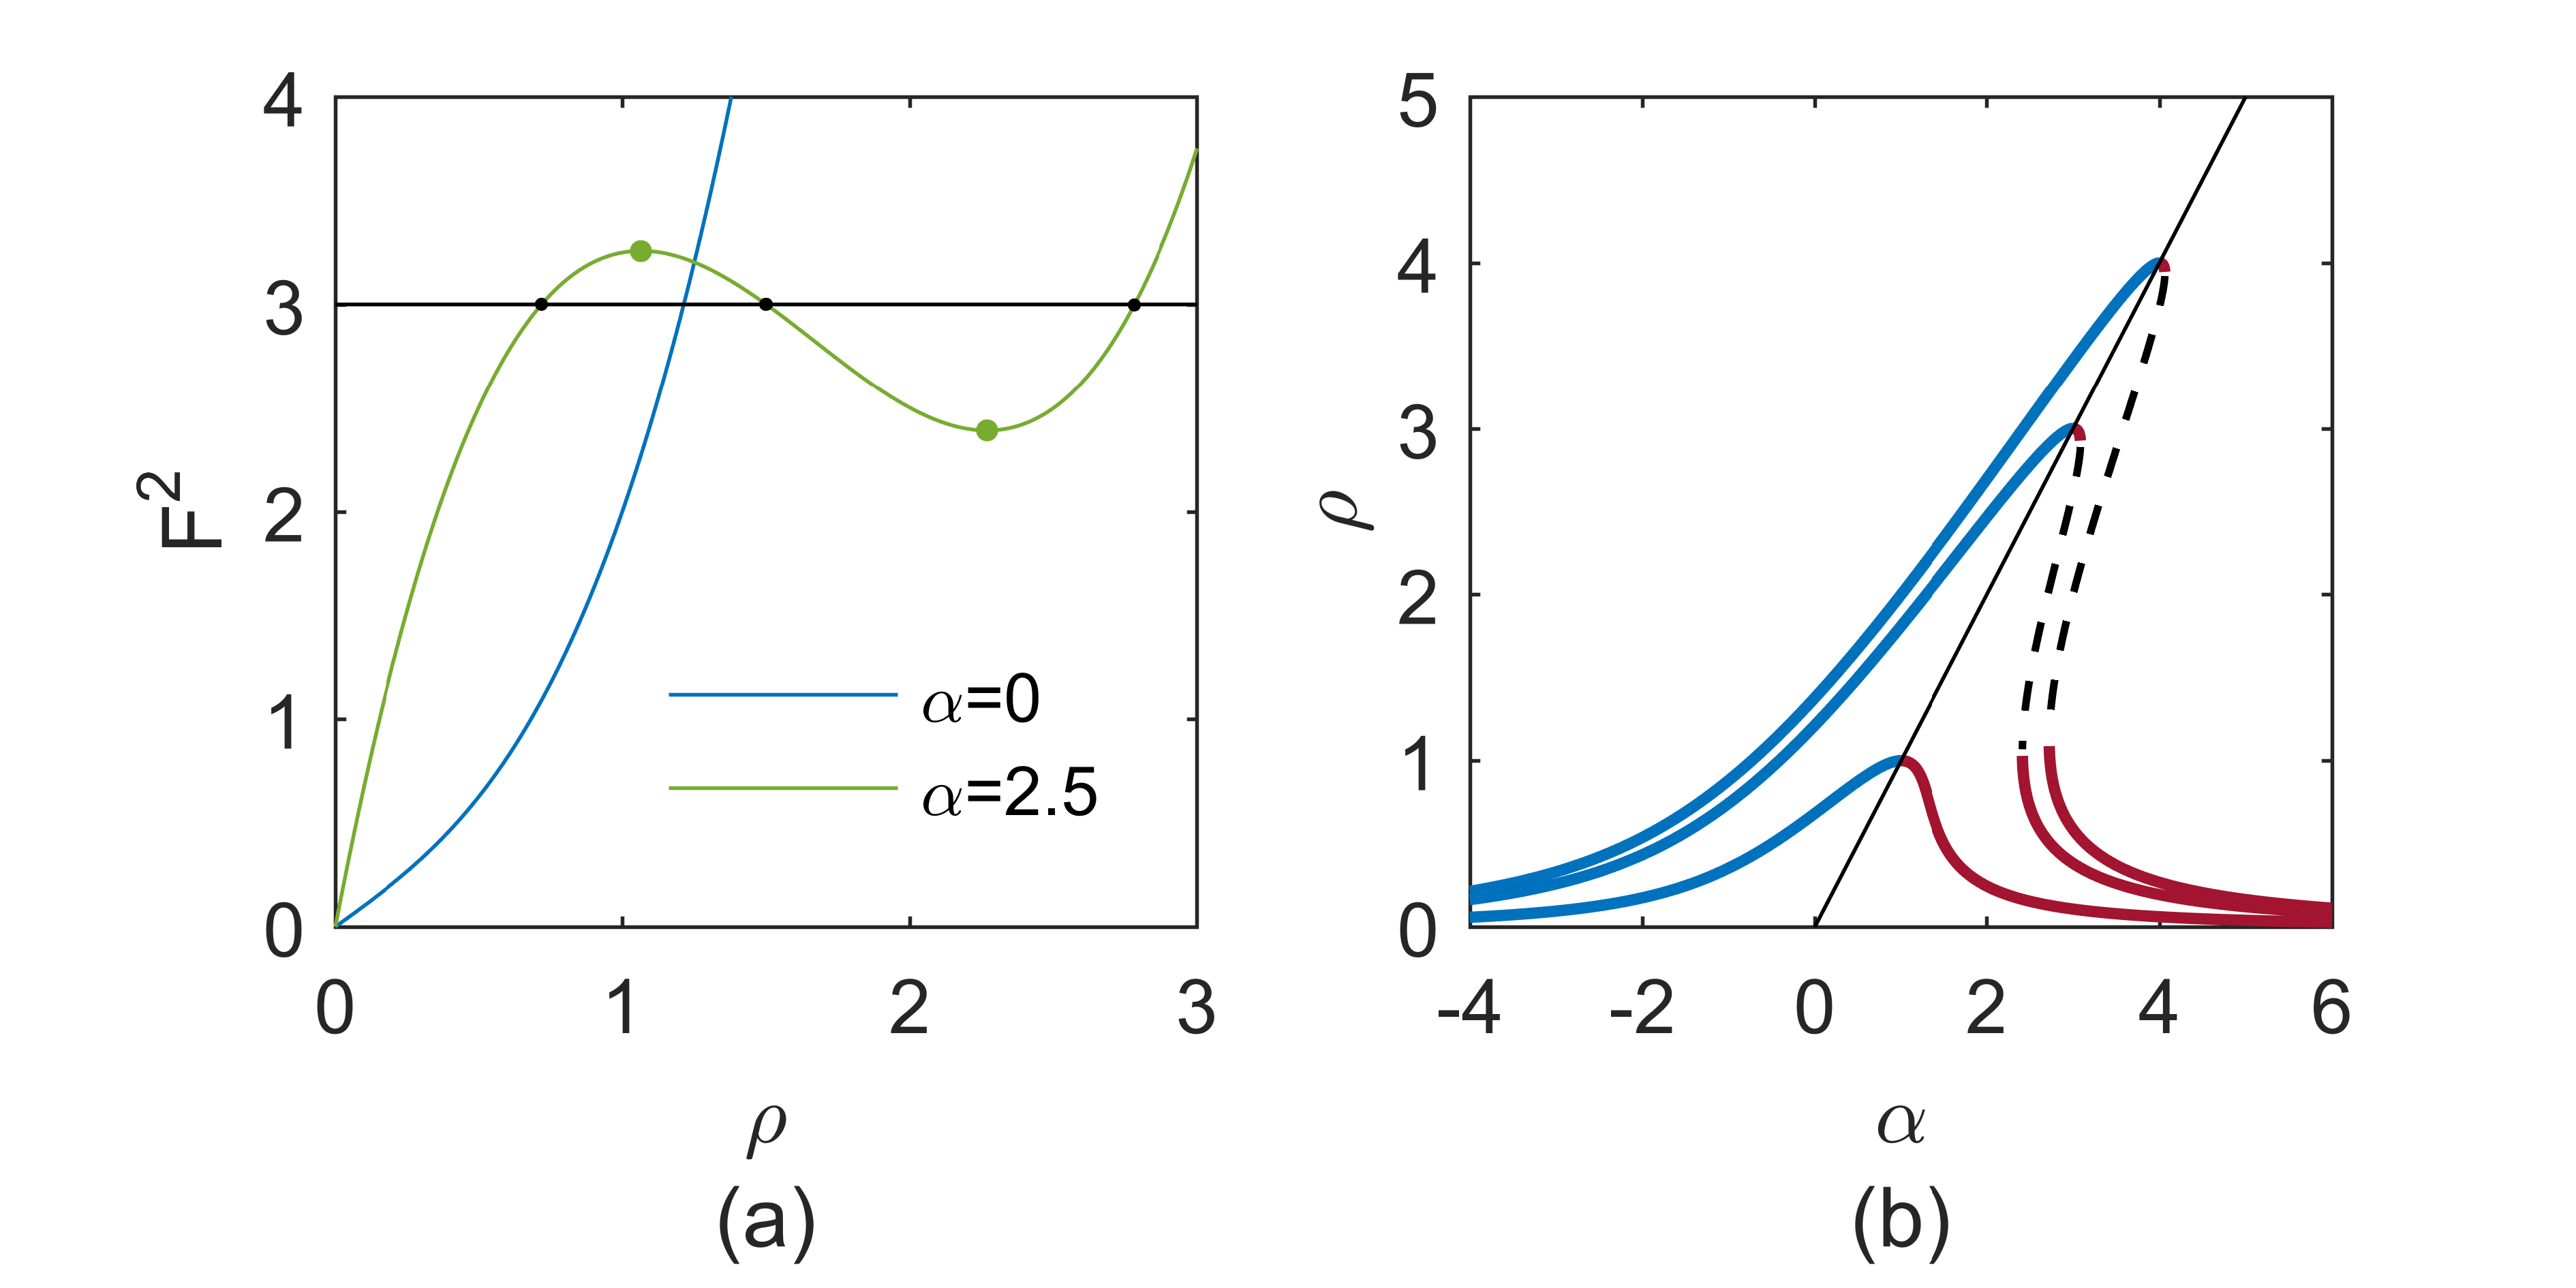
\includegraphics{\FigPath/Figures/Microresonators/MRcurves.png}
	\end{center}
	\caption[Investigation of the circulating CW power in a Kerr resonator]{\textbf{Investigation of the circulating CW power in a Kerr resonator.} (a) Plots of $F^2$ as a function of $\rho$ for $\alpha=0$ (blue) and $\alpha=2.5$ (green), according to Eq. \ref{eq:LLEstat2}. When real values of $\rho$ exist that extremize $F^2$ according to this equation, multiple real solutions for the circulating power $\rho$ exist between these extremal values of $F^2$. For $\alpha=2.5$ we indicate the extremal values of $F^2$ as green dots. For an example value $F^2=3$, the corresponding allowed values $\rho_1$, $\rho_2$, and $\rho_3$ are the intersections of the green curve and the black line (black dots); such a line would have three intersections with the green curve for any value of $F^2$ between $F^2_\alpha(\rho_-)$ and $F^2_\alpha(\rho_+)$. (b) Kerr-tilted resonances curves $\rho(\alpha)$ for $F^2=$1 (smallest), $F^2=$3, and $F^2=$4 (largest). The line $\rho=\alpha=F^2$ (solid black) marks the highest circulating power for a given input power $F^2$ and separates the effectively blue-detuned and effectively red-detuned branches. When $F^2>8\sqrt{3}/9$ (obtained by solving for $\rho_+=\rho_-$, Eq. \ref{eq:rhopm}), the resonance becomes tilted steeply enough that an unstable middle branch (dashed black) exists. }
	
	\label{fig:MRcurves}
\end{figure} 

Physically, the coexistence of multiple flat solutions $\rho$ at a given point $(\alpha,F^2)$ corresponds to a `tilting' of the Lorentzian transmission profile of the cavity and leads to bistability, even before taking into account thermal effects. This is illustrated in Fig. \ref{fig:MRcurves}. For flat solutions $\rho$, an effective Kerr-shifted detuning can be defined as $\alpha_{eff}=\alpha-\rho$. The effective detuning simply incorporates the Kerr nonlinearity into the round-trip phase shift that describes the constructive or destructive interference of the circulating field with the pump at the coupling port. By noting that $\alpha=F^2=\rho$ solves Eq. \ref{eq:LLEstat2}, we can conclude that the position of the effective Kerr-shifted resonance is on the line $\alpha=F^2$, where $\alpha_{eff}=0$. 

%For fixed $F^2$, an effectively red-detuned branch of the tilted resonance exists above the value of $\alpha$ where $\rho$ becomes multivalued. This value of $\alpha$ can be determined by inserting $\rho_-$ (Eq. {\ref{eq:rhopm}) into Eq. \ref{eq:LLEstat2} and solving for $\alpha$. 
	
%	The discussion of thermal effects in Sec. \ref{sec:thermaleffects} then applies to the effective detuning $\alpha_{eff}$; that is, operating with significant coupled power at \textit{effective} red detuning is thermally unstable, while thermal locking occurs with significant coupled power at effective blue detuning. 
	
%	Generally speaking, extended patterns exist on the upper branch of this curve, highlighted in blue, and solitons exist on the lower branch, highlighted in red. 

Once the circulating intensity $\rho$ is known, the corresponding flat solution $\psi_{CW}$ can be determined from Eq. \ref{eq:LLEstat} by inserting the known value of $\rho$ and solving for $\psi_{CW}$, with the result:
\begin{equation}
\psi_{CW}=\frac{F}{1+i(\alpha-\rho)}.\label{eq:LLEflatsoln}
\end{equation}
This expression reveals that the flat solution acquires a phase $\phi_s=\tan^{-1}(\rho-\alpha)$ relative to the pump.


%By introducing a perturbation $\delta\psi$ to the flat solution $\psi_s$ and solving for the time evolution of the perturbation, the stability of the flat solution can be investigated---a flat solution $\psi_s$ to the LLE only corresponds to a physically-realizable CW resonator background if it is stable to perturbations. We don't reproduce this analysis in detail here, but state the result:

If the flat solution(s) at a point $(\alpha,F^2)$ is (are) unstable, a Kerr comb will form spontaneously. Stability analysis of the flat solutions can be performed, and for the case of second-order dispersion alone the results are \cite{Godey2014}:
\begin{itemize}
	\item In the region of multi-stability, if the flat solutions are ordered with increasing magnitude as $\rho_1$, $\rho_2$, and $\rho_3$, the middle solution $\rho_2$ is always unstable. 
	\item When $\alpha<2$, a flat solution $\rho$ that is not the middle solution is stable if $\rho<1$; otherwise it is unstable. When the flat solution is unstable, the mode that experiences the greatest instability has mode number given by:
	\begin{equation}
\mu_{max}=\sqrt{\frac{2}{\beta_2}(\alpha-2\rho)}  \label{eq:mumax}
	\end{equation} 
\end{itemize}

Therefore, the pump-laser threshold curve for Kerr-comb generation can be determined in the region $\alpha<2$ of the $\alpha-F^2$ plane by setting $\rho=1$ in Eq. \ref{eq:LLEstat}: 
\begin{equation}
F^2_{thresh}=1+(\alpha-1)^2, \label{eq:F2thresh}
\end{equation}
\begin{equation}
\alpha_{thresh,\pm}=1\pm\sqrt{F^2-1}. \label{eq:alphathresh}
\end{equation}
These equations explicitly describe the point at which comb is generated in an experiment in which the pump power or detuning is varied while the other is held fixed. 



\subsection{Kerr comb outputs: extended modulation-instability patterns}

Extended temporal patterns arise spontaneously as a result of the instability of the flat solution to the LLE when the pump laser is tuned above the threshold curve. Two types of extended patterns are shown in Fig. \ref{fig:MRextendedpatterns}. These patterns can be stationary, in which case they are typically referred to as `Turing patterns' or `primary comb,' or can evolve in time, in which case they are typically referred to as `noisy comb' or `spatiotemporal chaos.' In general, the former occurs for lower values of the detuning $\alpha$ and smaller pump strengths $F^2$; although some studies of the transition from Turing patterns to chaos have been conducted (e.g. Ref. \citeNoBrackets{Coillet2014}), a well-defined boundary between the two has not been established, and may not exist. 

In the spatial domain parametrized by $\theta$, a Turing pattern consists of a pulse train with (typically) $n\gg1$ pulses in the domain $-\pi\leq\theta\leq\pi$---the pulse train's repetition rate is a multiple of the cavity FSR: $f_{rep}=n\times f_{FSR}$. Corresponding to the $n$-fold decreased period (relative to the round-trip time) of an $n$-pulse Turing pattern's modulated waveform in the time domain, the optical spectrum of a Turing pattern consists of modes spaced by $n$ resonator FSR---it is this widely-spaced spectrum that is referred to as `primary comb.'  Analytical approximations for Turing patterns are possible near threshold \cite{Lugiato1987,Lugiato1987a} and in the small damping limit \cite{Renninger2016}. The stability analysis results from the last section can be used to predict the spacing $n$ of a primary comb (equivalently the number of Turing-pattern pulses) generated in a decreasing-frequency scan across the resonance with fixed normalized pump power $F^2$:
\begin{equation}
n=\mu_{max,thresh}=\sqrt{\Delta\omega_0(1+\sqrt{F^2-1})/D_2},
\end{equation}
which is obtained by inserting $\alpha_{thresh,-}$ from Eq. \ref{eq:alphathresh} and $\rho=1$ into the expression for $\mu_{max}$ in Eq. \ref{eq:mumax} above and moving to the dimensionful dispersion parameter $D_2$. Fig. \ref{fig:MRextendedpatterns}a shows measured and simulated primary comb spectra and Fig. \ref{fig:MRextendedpatterns}b shows the corresponding simulated time-domain waveform.

Spatiotemporal chaos can be understood as a Turing pattern whose pulses oscillate in height, with adjacent pulses oscillating out of phase. From such an oscillating Turing pattern, if $\alpha$ and/or $F^2$ is increased, one moves deeper into the chaotic regime and pulses begin to exhibit lateral motion and collisions; the number of pulses present in the cavity is no longer constant in time. Depending on the severity of the chaos (greater for larger $\alpha$ and $F^2$), a chaotic comb may correspond to a primary-comb-type spectrum with each primary-comb mode exhibiting sidebands at the resonator FSR, so-called `subcombs,' or it may correspond to a spectrum with light in each cavity mode. Fig. \ref{fig:MRextendedpatterns}c shows measured and simulated time-averaged spectra of chaotic combs and Fig. \ref{fig:MRextendedpatterns}d shows a corresponding simulated time-domain waveform.

\begin{figure}[htpb]
	\begin{center}
		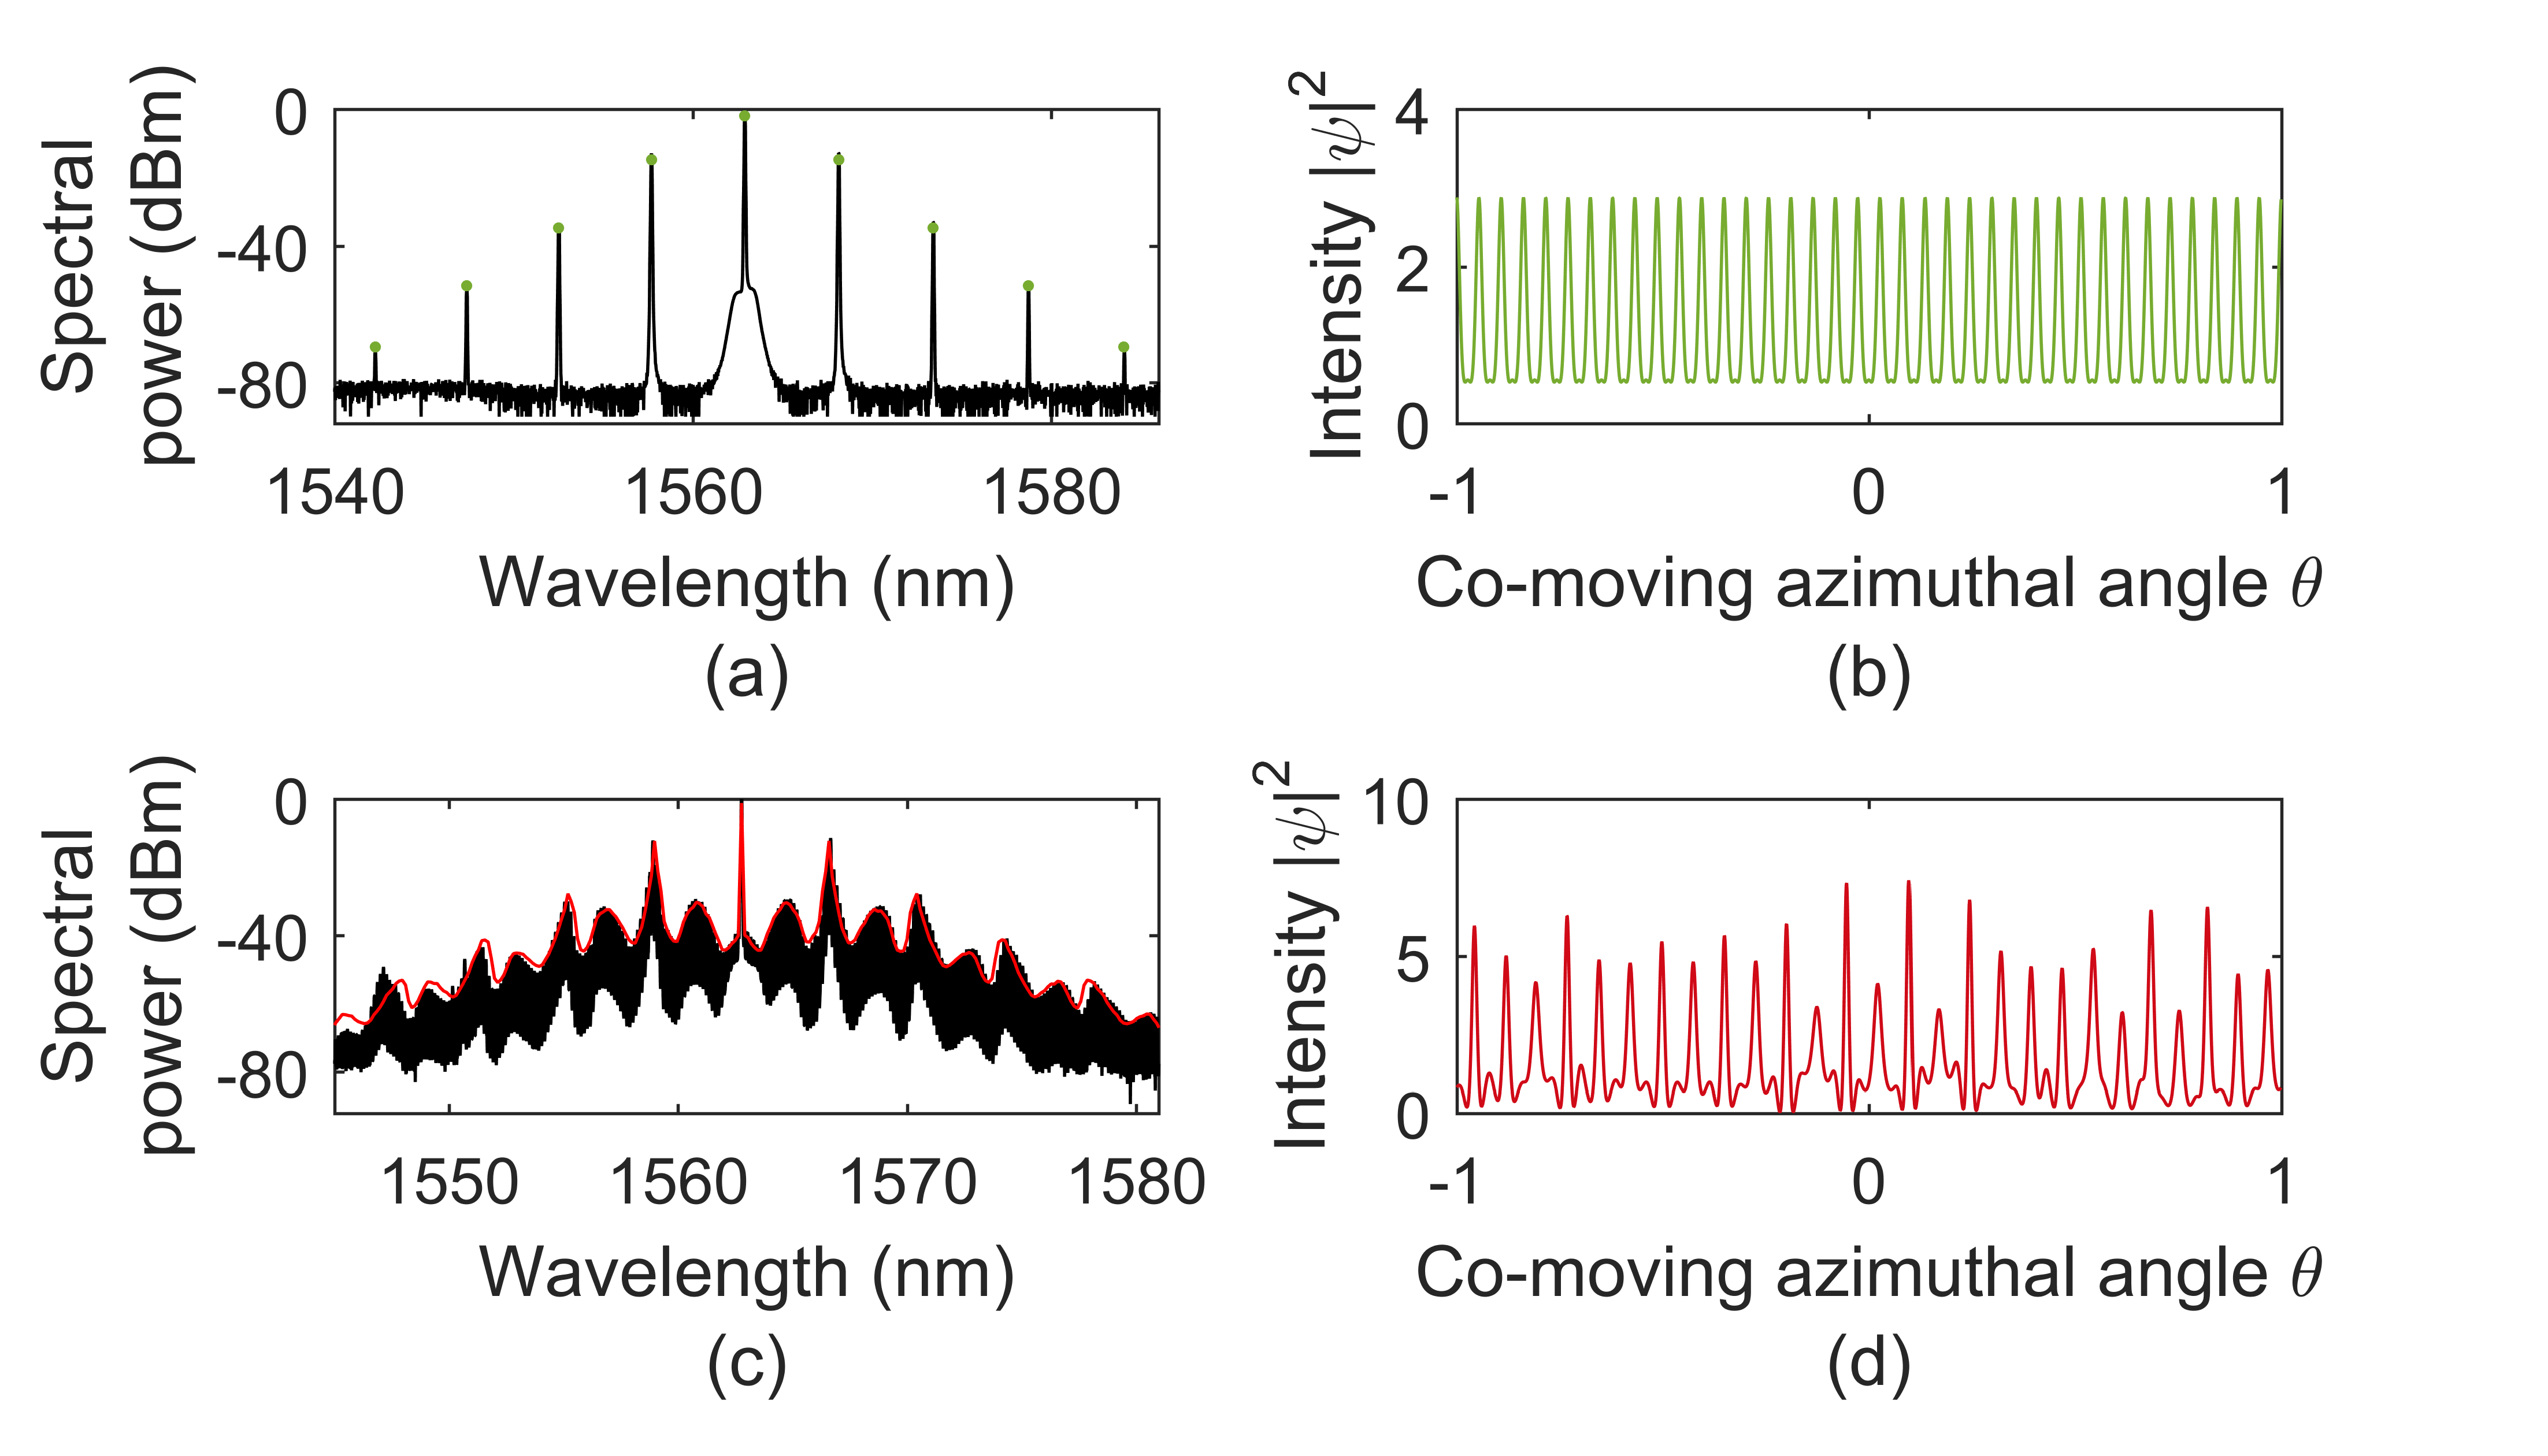
\includegraphics{\FigPath/Figures/Microresonators/MRextendedpatterns.png}
	\end{center}
	\caption[Extended-pattern solutions to the LLE]{\textbf{Extended-pattern solutions to the LLE.} (a,b) Primary-comb pulse train in the frequency (a) and time (b) domains. The primary-comb spectrum corresponds to 39 time-domain pulses. The experimental optical spectrum (black) was obtained in a microdisk resonator with 17.32 GHz free-spectral range, and the simulation (green) is conducted with parameters near typical experimental values: $F^2$=6, $\alpha=-0.6$, and $\beta_2=-0.0044$. (c,d) Spatiotemporal chaos obtained in the same resonator. The experimental measurement (black) yields a time-averaged optical spectrum, with a simulation of qualitatively similar dynamics shown in red. Simulation parameters are $F^2=4.2$, $\alpha=1.2$, and $\beta_2=-0.0054$. A snapshot of the evolving time-domain waveform is shown in (d).
	}
	
	\label{fig:MRextendedpatterns}
\end{figure} 

Relative to generation of solitons, discussed below, experimental generation of an extended pattern is straightforward. These patterns are generated with blue effective pump-laser detuning $\alpha_{eff}<0$, where thermal locking can occur. Because they arise spontaneously from noise, their generation is (comparatively) straightforward: simply decrease the pump-laser frequency until a pattern is generated. Unfortunately, operation of a Kerr-comb in the extended pattern regime is disadvantageous for applications: the $n$-FSR spacing of primary comb presents a challenge for measurement of the repetition rate of the frequency comb due to the bandwidth of measurement electronics and is also an inefficient use of physical space (i.e. for an $n-$pulse primary comb pulse train, an equivalent pulse train can always be obtained using the single-soliton output of a resonator with area that is smaller by a factor of $1/n^2$), and the aperiodic time-evolution of chaotic comb corresponds to modulation sidebands on the comb modes within the linewidth of the cavity that preclude the use of the comb as a set of stable optical reference frequencies. 

An important property of these extended patterns is that they fill the resonator---the characteristic size of temporal features scales roughly as $1/\sqrt{-\beta_2}$, but these features are distributed densely and uniformly throughout the resonator. This means that the total circulating power of an extended pattern $\int d\theta\, |\psi|^2$ is large relative to the localized pulses discussed in the next section, and therefore that extended patterns come with a comparatively large thermal shift of the resonance. As explained below, this contributes to the experimental challenges in soliton generation.



\subsection{Kerr comb outputs: solitons} \label{sec:LLEsolitons}
The term `soliton' generally refers to a localized excitation that can propagate without changing its shape due to a delicate balance between dispersion (or diffraction) and nonlinearity; sometimes known as `solitary waves,' solitons entered the scientific consciousness in the nineteenth century with their observation by John Scott Russell \cite{Russell1844}. They are fundamental solutions to nonlinear partial-differential equations that describe a host of physical phenomena, and are found in several contexts within the field of nonlinear optics: spatial\cite{Lugiato1987,Brambilla1997} and spatiotemporal solitons (light bullets) \cite{Minardi2010} have been studied, and soliton modelocking \cite{Kartner1996,Grelu2012} is an important method of femtosecond pulse generation. Temporal Kerr-soliton pulses in optical fibers are particularly well known \cite{Agrawal2007,Mollenauer2006}, and have been considered as a candidate for fiber-optic communications protocols \cite{Hasegawa1995,Haus1996}. Microresonators support so-called dissipative cavity solitons, which are localized pulses circulating the resonator that are out-coupled once per round trip. In the case of a single circulating soliton, this leads to a train of pulses propagating away from the resonator with repetition rate $1/T_{RT}$. Thus the mode spacing of the comb matches the FSR of the resonator, in contrast with widely-spaced primary comb spectra, and the soliton can, in principle, remain stable and propagate indefinitely as a stationary solution to the LLE. This makes Kerr combs based on solitons particularly attractive for applications.

\subsubsection{Mathematical description of solitons}
\label{sec:solitonmath}

Solitons in optical fibers are solutions of the nonlinear Schrodinger equation (NLSE) that describes pulse-propagation in optical fiber \cite{Agrawal2007}:
\begin{equation}
\frac{\partial A}{\partial z}= i\gamma|A|^2 A -i \frac{k''}{2} \frac{\partial^2 A}{\partial T^2}. \label{NLSE}
\end{equation}
This equation describes the evolution of the pulse envelope $A$ in the `fast-time' reference frame parametrized by $T$ as it propagates down the length of the fiber, parametrized by the distance variable $z$. Here $\gamma=\frac{2\pi}{\lambda}\frac{n_2}{A_{eff}}$ is the nonlinear coefficient of the fiber, where $n_2$ is the Kerr index, $A_{eff}$ is the effective nonlinear mode area and $\lambda$ is the carrier wavelength, and $k''<0$ is the GVD parameter. The LLE can be viewed as an NLSE with additional loss and detuning terms $-(1+i\alpha)\psi$ and a driving term $F$.

The fundamental soliton solution to the NLSE is:
\begin{equation}
A_{sol}=\sqrt{P_0}\, \mathrm{sech}\left(T/\tau\right)\,e^{i\gamma P_0 z/2+i\phi_0},
\end{equation}
where $P_0$ is the peak power of the pulse and is related to the duration of the pulse $\tau$ via $\tau=\sqrt{-l''/\gamma P_0}$, and $\phi_0$ is an arbitrary phase. Thus, this equation admits a \textit{continuum} of pulsed fundamental `soliton' solutions, with one existing for each value of the peak power. Each of these solutions propagates down the fiber without changing shape; only the phase evolves with distance as $\phi(z)=\gamma P_0 z/2+\phi_0$.


The introduction of the loss, detuning, and driving terms into the NLSE to obtain the LLE has several important consequences for solitons. First, exact analytical expressions for the soliton solution to the LLE in terms of elementary functions are not known, in contrast with the situation for the NLSE. However, the soliton solutions to the LLE, Eq. \ref{eq:LLE}, can be approximated well as:
\begin{equation}
\psi_{sol}=\psi_{CW,min}+e^{i\phi_0}\sqrt{2\alpha}\,\mathrm{sech}\sqrt{\frac{2\alpha}{-\beta_2}}\theta. \label{eq:LLEsoliton}
\end{equation}
Here $\psi_{CW,min}$ is the flat solution to the LLE from Eq. \ref{eq:LLEflatsoln} at the point where the soliton solution is desired; when multiple flat solutions exist, $\psi_{CW,min}$ is the one corresponding to the smallest intensity $\rho_1$. The phase $\phi_0=\mathrm{cos}^{-1}(\sqrt{8\alpha}/\pi F)$ arises from the intensity-dependent phase shift in the cavity due to the Kerr effect, mathematically described by the term $i|\psi|^2\psi$. We depict this approximation, alongside numerical calculations of exact soliton solutions to the LLE, in Fig. \ref{fig:MRsoliton}.

%\footnote{Perhaps its worth noting that this is a mathematical approximation, in the sense that this is simply a way to approximate the steady-state solution to a differential equation that we don't know how to solve with elementary functions. There isn't any obvious physical approximation we make (e.g. ignoring some particular effect or taking a particular limit) in moving from the exact numerical soliton solution to Eq. \ref{eq:psisol}}

\begin{figure}[htpb]
	\begin{center}
		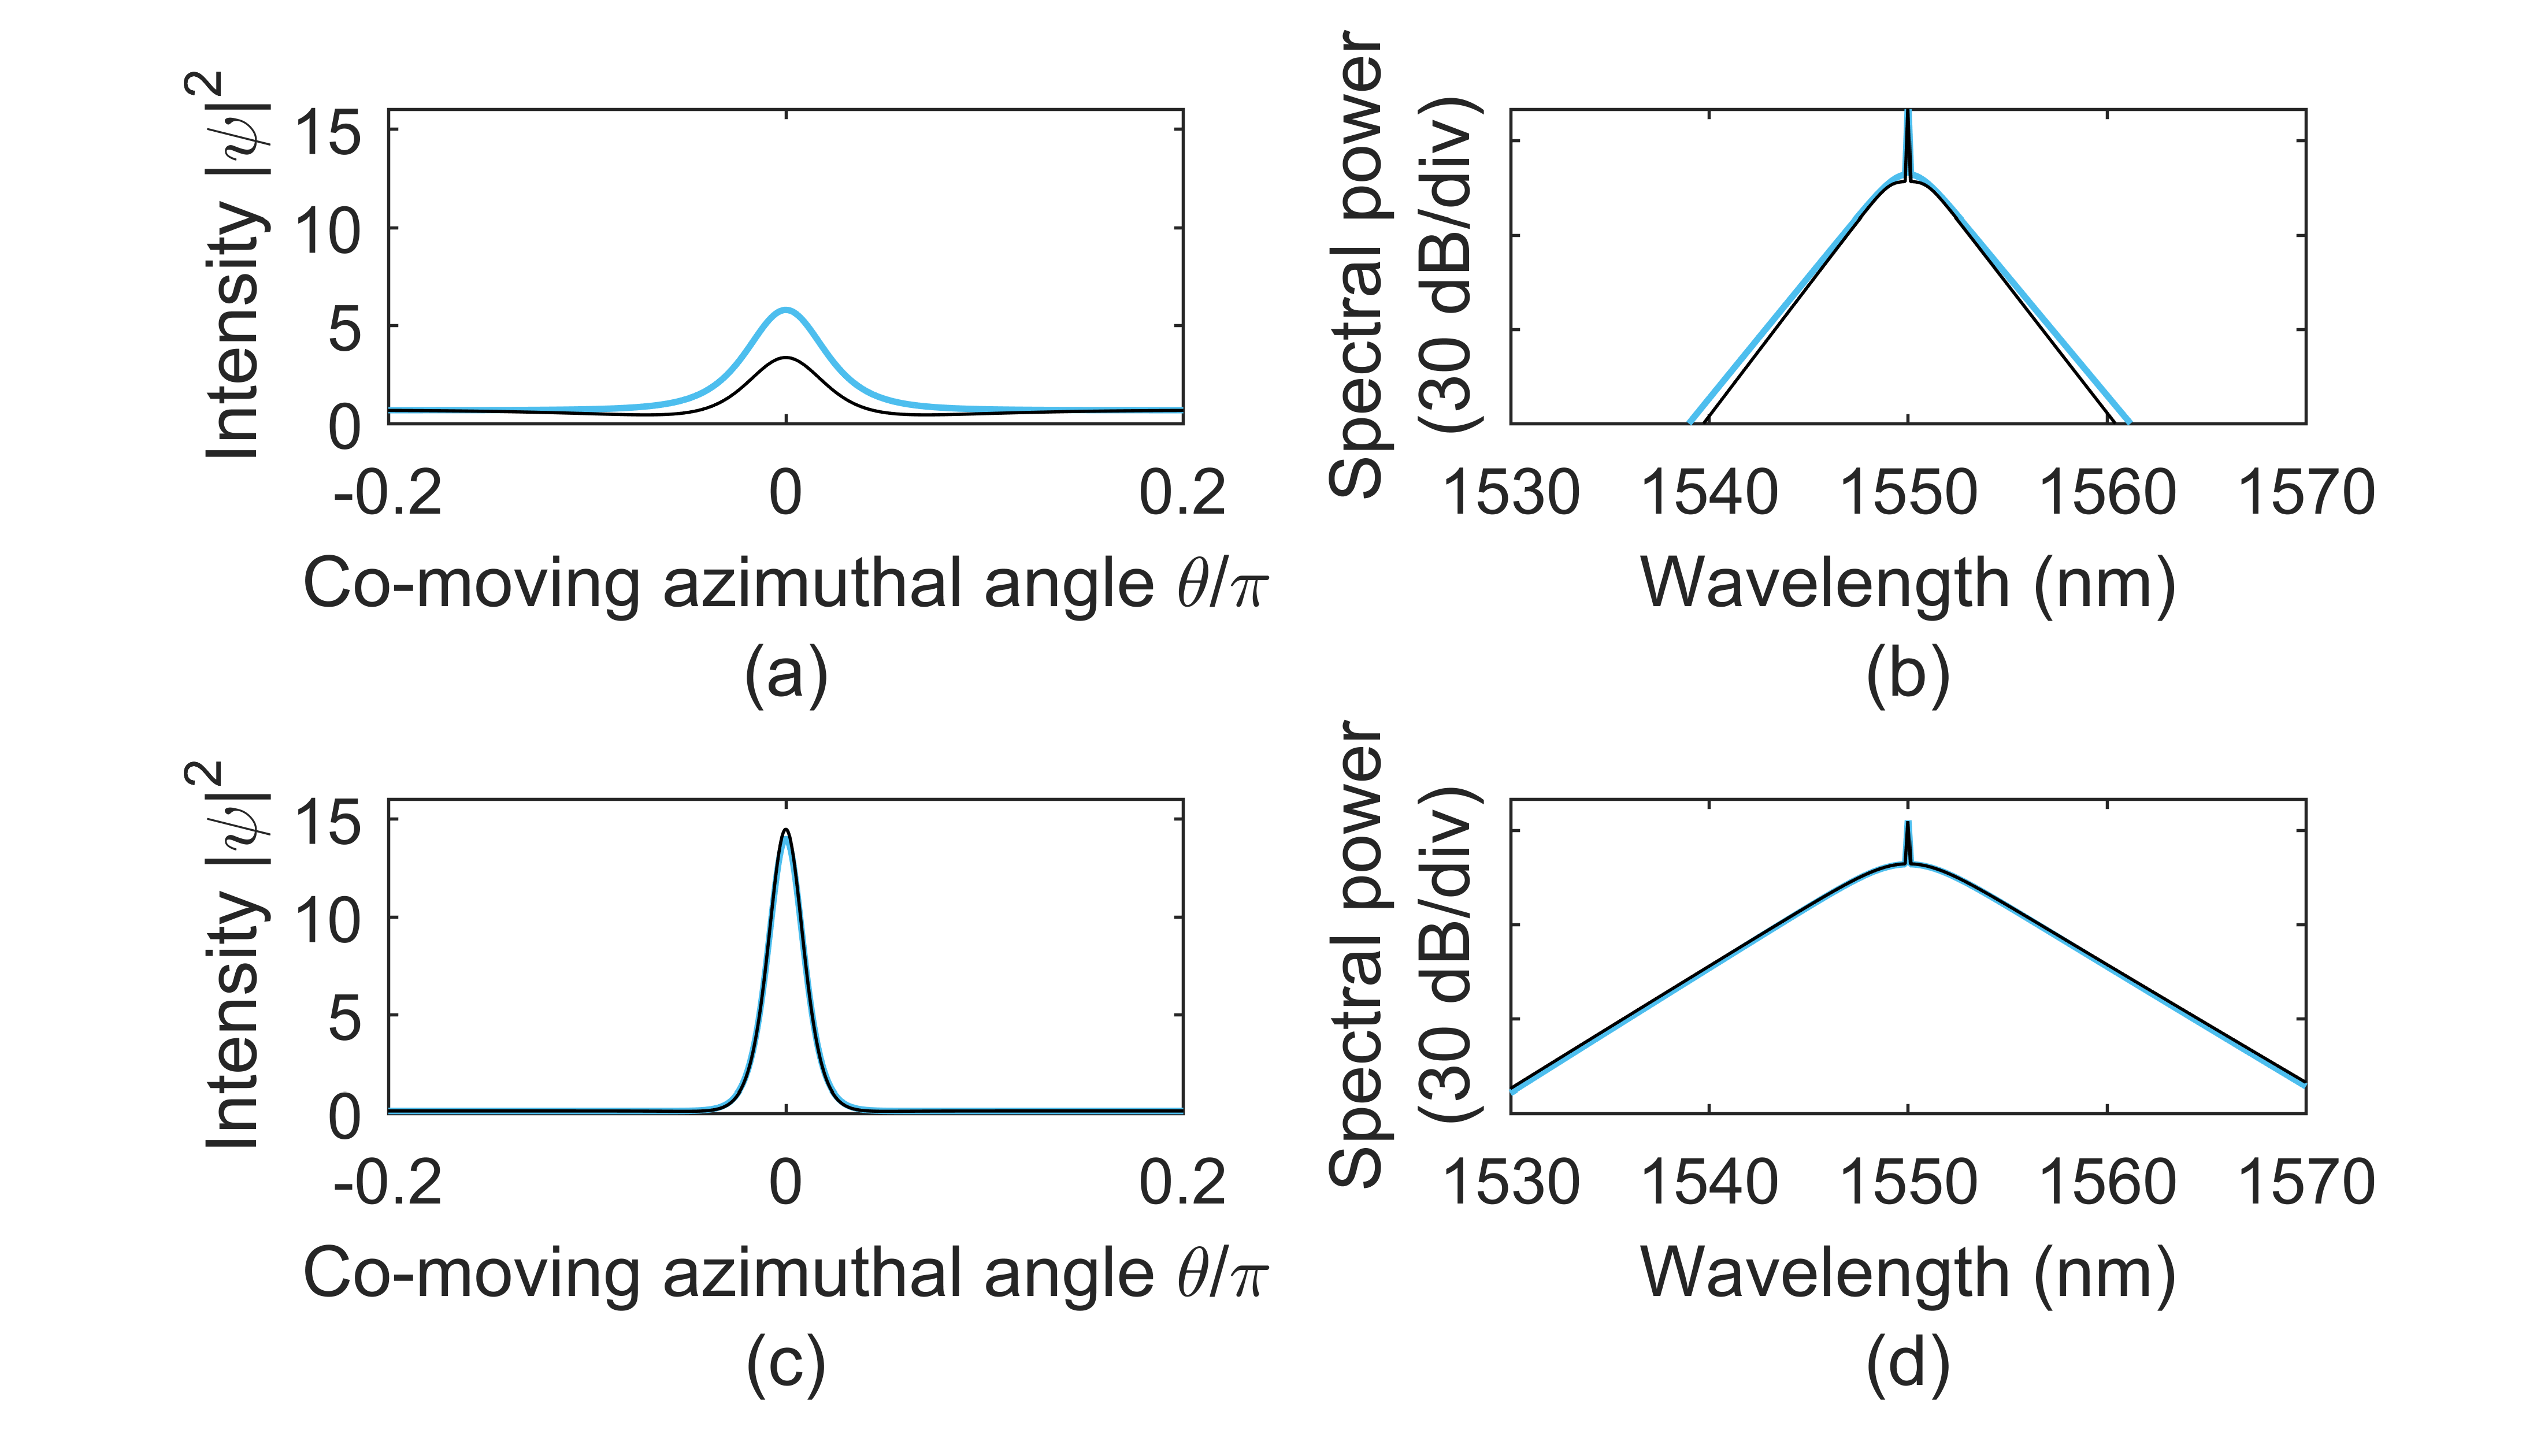
\includegraphics{\FigPath/Figures/Microresonators/MRsoliton.png}
	\end{center}
	\caption[Soliton solutions to the LLE]{\textbf{Soliton solutions to the LLE.} Analytical approximations (color) and numerically-calculated exact solutions (black) to the LLE in the time (a,c) and frequency (b,d) domains. The solitons are calculated at $\alpha=0.95\,\alpha_{max}=0.95\,\pi^2F^2/8$ for $F^2=8\sqrt{3}/9$ (a,b) and $F^2=6$ (c,d) with $\beta_2=-0.02$ in both cases. The isolated spectral spike is at the pump frequency and corresponds to the CW background $\psi_{CW,min}$. Spectra are calculated using $f_{rep}=$16.5 GHz with pump wavelength of $\lambda_p$=1550 nm. For experimental measurements of solitons in microring resonators, see Chapters \ref{chap:PMPumping} and \ref{chap:SolitonCrystals}.
	}
	
	\label{fig:MRsoliton}
\end{figure} 


This approximation $\psi_{sol}$ from Eq. \ref{eq:LLEsoliton} for the soliton solution of the LLE illustrates a second important consequence of the differences between the NLSE and the LLE: while the NLSE admits a continuum of fundamental soliton solutions parametrized by their peak power $P_0$ and arbitrary phase $\phi_0$, the LLE supports only one shape for the envelope of a soliton for fixed experimental parameters.  Intuitively, this can be understood as arising from the need for the round-trip phase shift for all points on the soliton to be zero in steady-state; the introduction of the detuning parameter $\alpha$ breaks the degeneracy that exists for the NLSE within the continuum of soliton solutions.

The analytical approximation in Eq. \ref{eq:LLEsoliton} indicates the scaling of the amplitude and width of the LLE soliton with the experimental parameters: the amplitude of the LLE soliton, prior to its summation with the CW background, depends only on the detuning $\alpha$, and the width of the soliton increases with larger detuning $\alpha$ and smaller dispersion $\beta_2$. Importantly, if one is concerned with maximizing the bandwidth of the soliton, it is important to minimize $\beta_2$ and maximize $\alpha$, due to the inverse relationship between temporal duration and spectral bandwidth. The spectrum of a single-soliton Kerr comb has a $\mathrm{sech}^2\left((\omega-\omega_p)/\Delta \omega_{sol}\right)$ envelope, where $\omega$ is the optical angular frequency and $\Delta\omega_{sol}\approx\sqrt{32\alpha/|\beta_2| T_{RT}^2 }$ is the bandwidth of the pulse in angular frequency. Equivalently, the bandwidth of the soliton in (linear) optical frequency is $\sqrt{\frac{16\Delta\nu f_{rep}^2}{D_2}\alpha}$, where $\Delta\nu$ is the resonance linewidth in linear frequency; the spectral width in mode number is $\Delta\mu_{sol}\approx4\sqrt{\alpha\Delta\nu/D_2}$. Consistent with the phase $\phi_0$ in the approximation $\psi_{sol}$ in Eq. \ref{eq:LLEsoliton}, solitons can exist up to a maximum detuning of $\alpha_{max}\sim\pi^2 F^2/8$ \cite{Herr2014}. For a soliton at the maximum detuning for fixed normalized pump power $F^2$, the bandwidth is then $\sqrt{\frac{\pi^2\Delta\nu f_{rep}^2}{2 D_2}F^2}$. 

Solitons exist only where there is a stable flat solution $\psi_{CW}$ that is effectively red detuned that can form the background for the pulse \cite{Barashenkov1996,Coen2013}. This effectively red-detuned background is itself thermally unstable (see Sec. \ref{sec:thermaleffects}), but the existence of the soliton acts to stabilize the pump detuning. As explained by Herr et al., the soliton provides a local modulation of the refractive index through the Kerr effect, which changes the round-trip phase shift of pump light that arrives coincidentally with the soliton at the coupling port \cite{Herr2014}. This leads to a \textit{local} increase in the resonant wavelength for this pump light. Thus there are effectively two resonant wavelengths, a smaller one determined by the round-trip phase shift including the Kerr shift from the CW background, and a larger one determined by the round-trip phase shift including the Kerr shift from the soliton \cite{Guo2017a}. The pump laser can be effectively blue-detuned with respect to the latter resonance, which can lead to thermally stable operation in the soliton regime.

%is clearly valid only for red pump-laser detuning  Solitons exist as solutions to the LLE only for red pump-laser detuning $\alpha>0$.

Solitons are strongly localized: as can be seen from Eq. \ref{eq:LLEsoliton}, the deviation of the background intensity from $\rho_1$ near a soliton at $\theta_0$ is proportional to $e^{-(\theta-\theta_0)/\delta\theta}$, where $\delta\theta=\sqrt{-\beta_2/2\alpha}$. If $\delta\theta$ is sufficiently small, multiple solitons can be supported in the resonator domain $-\pi\leq\theta\leq\pi$ with very weak interactions between solitons. If the separation between solitons $i$ and $j$ at $\theta_i$ and $\theta_j$ is small relative to $\delta\theta$, the solitons will interact. The topic of soliton interactions is complicated in general, with different types of interactions in different systems (see e.g. Refs. \cite{Zabusky1965,Gordon1983,Malomed1991,Jang2013}). Simulations reveal that if $(\theta_i-\theta_j)/\delta\theta$ is too small, LLE solitons exhibit attractive interactions as a result of the monotonic (as opposed to oscillatory) decay of the localized pulse to $\psi_{CW}$ \cite{Parra-Rivas2017}, which precludes the existence of stable equilibrium separations. The result of this attraction can be pair-wise annihilation or merger, with the ultimate result being an ensemble with fewer solitons. The maximum number of solitons that can coexist in a resonator in the absence of higher-order stabilizing effects (see Chapter \ref{chap:SolitonCrystals} and Refs. \cite{Wang2017,Parra-Rivas2017}) can be approximated as $N_{max}\approx\sqrt{-2/\beta_2}$ \cite{Herr2014}. An approximation to the form of a soliton ensemble is possible as:

\begin{equation}
\psi_{ens}=\psi_{CW,min}+e^{i\phi_0}\sqrt{2\alpha}\sum_j \mathrm{sech}\left(\sqrt{\frac{2\alpha}{-\beta_2}}(\theta-\theta_j)\right),\label{eq:LLEsolens}
\end{equation}
where $\{\theta_j\}$ define the positions of the solitons in the ensemble and $\phi_0=\mathrm{cos}^{-1}(\sqrt{8\alpha}/\pi F)$ as above. Fig. \ref{fig:MRenergylevels} provides an example illustrating the degeneracy in soliton number of Kerr-combs operating in the soliton regime.

\begin{figure}[htpb]
	\begin{center}
		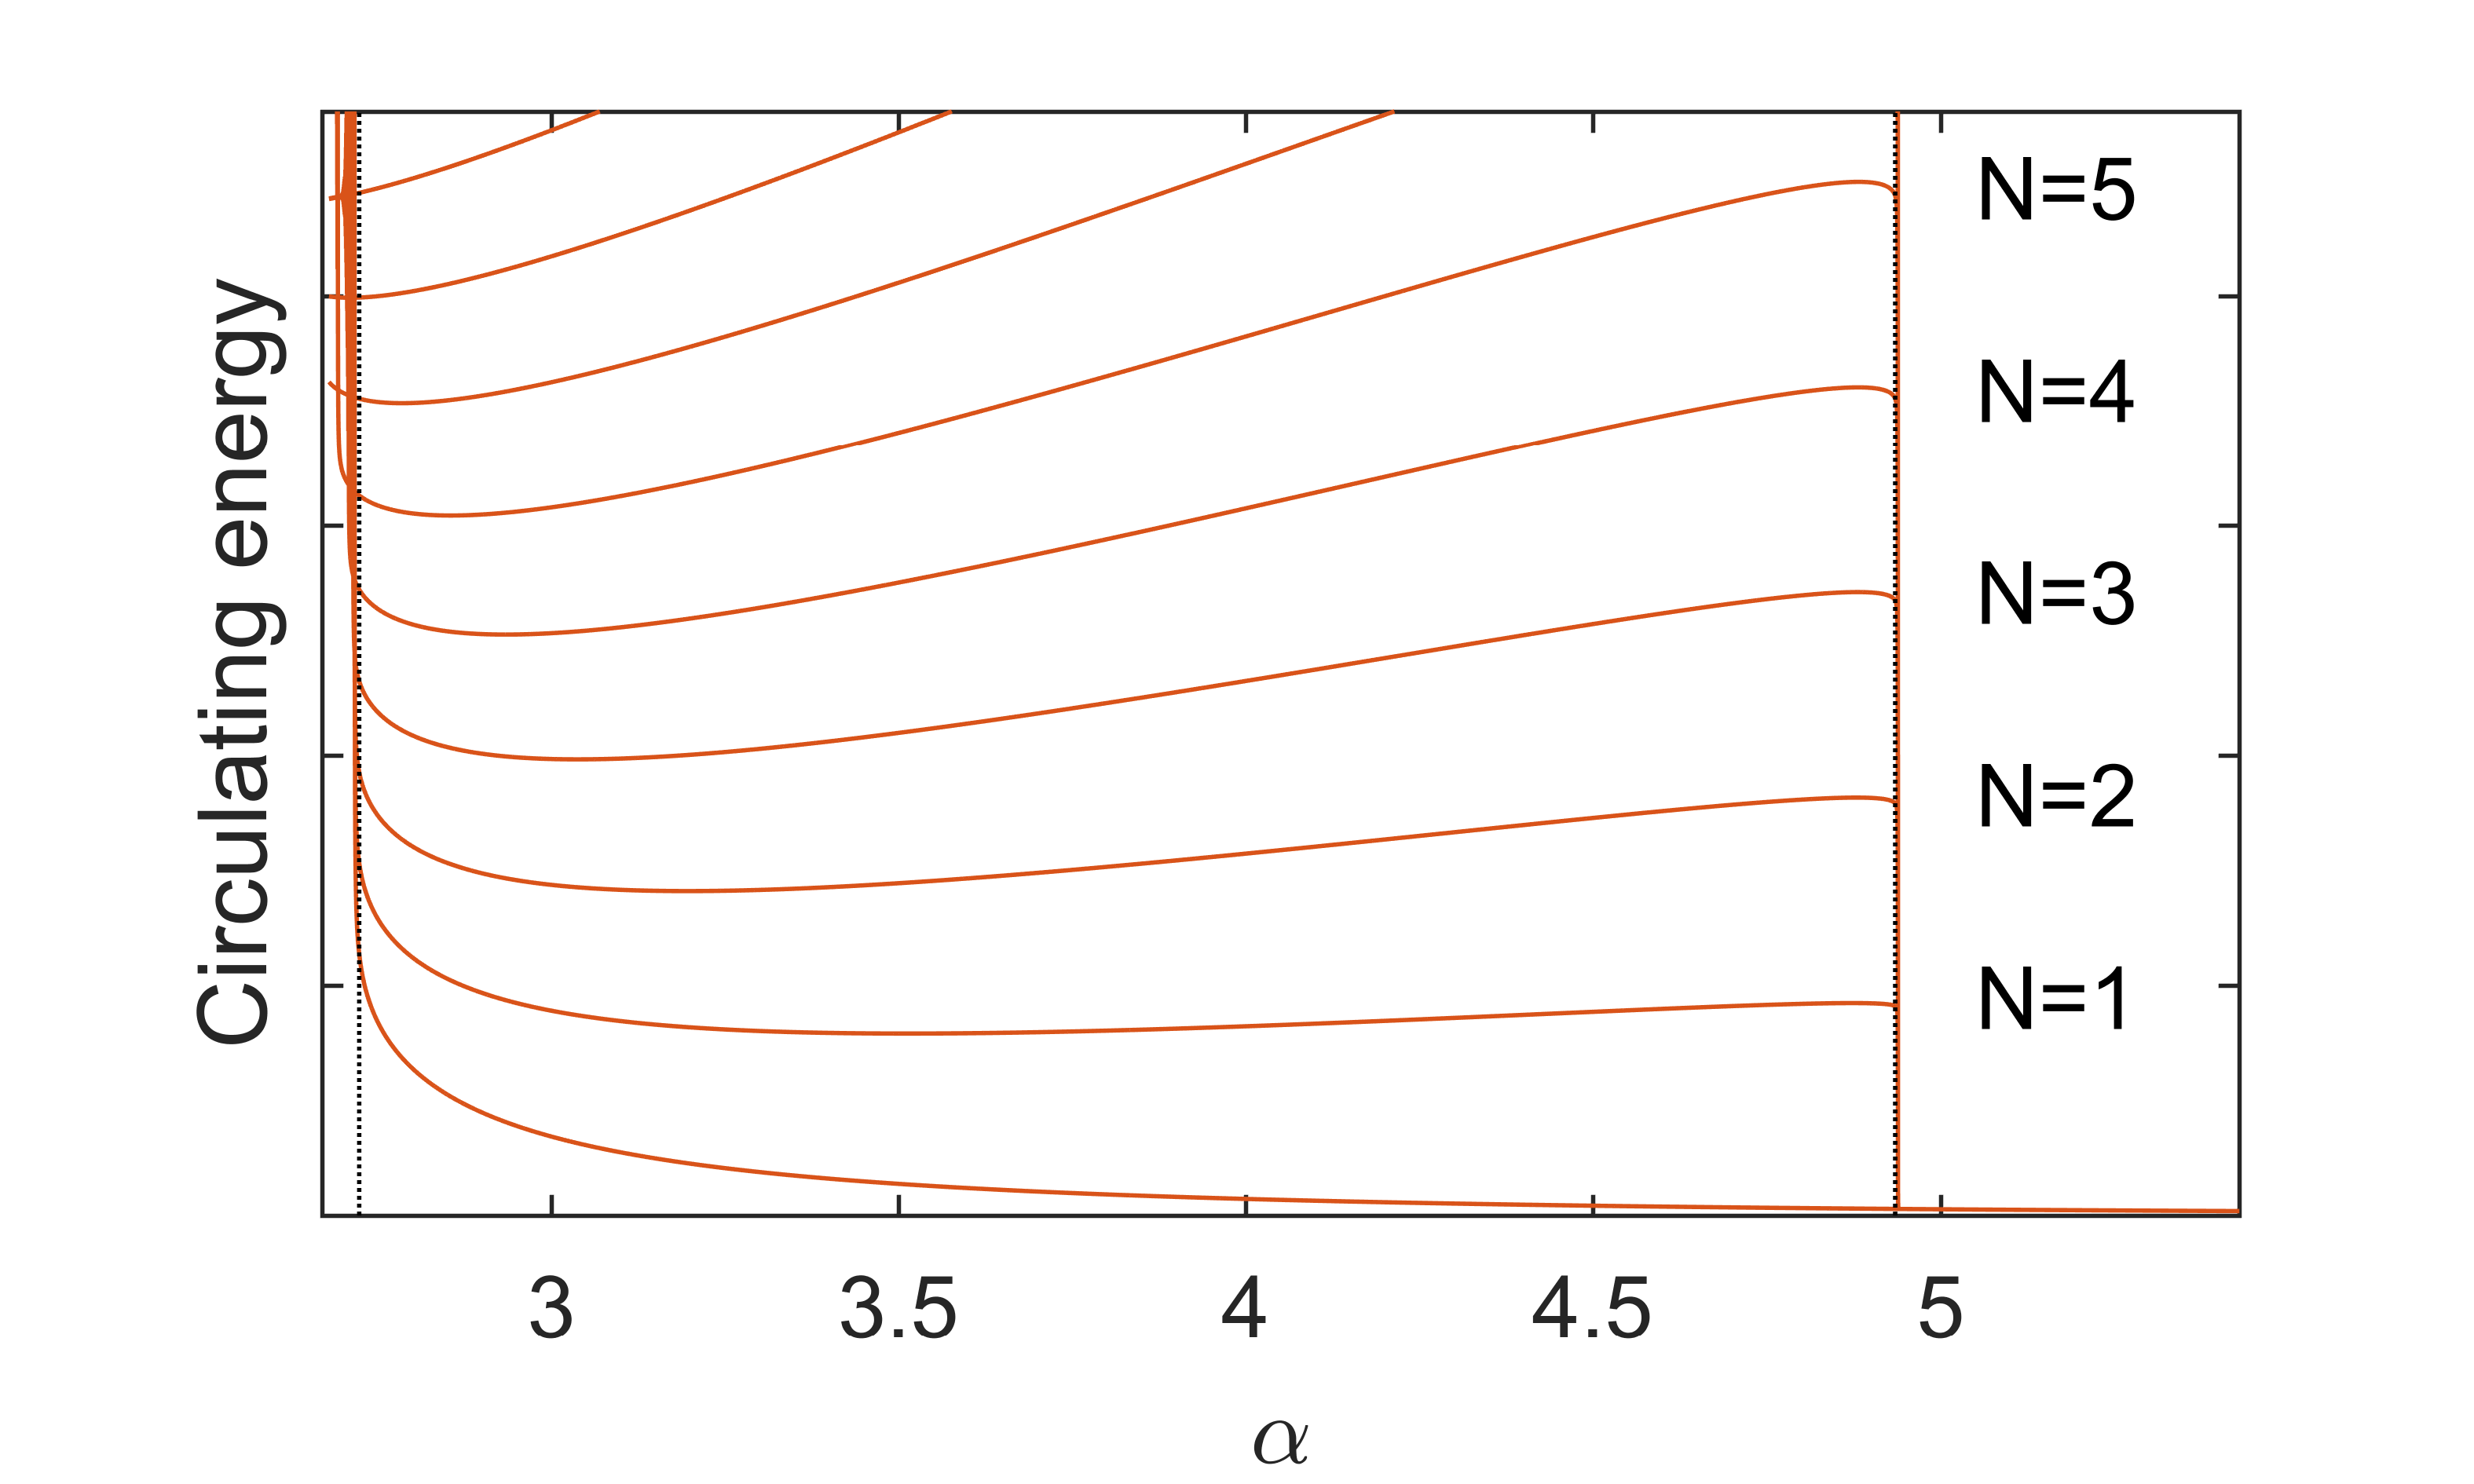
\includegraphics{\FigPath/Figures/Microresonators/MRenergylevels_slower.png}
	\end{center}
	\caption[Kerr-soliton energy-level diagram]{\textbf{Kerr-soliton energy-level diagram.} Some of the possible values of the circulating energy (proportional to $\int d\theta\,|\psi|^2$) in the soliton regime as a function of the detuning parameter $\alpha$. Level curves correspond to the number of circulating solitons. This diagram is obtained from numerical solutions using $F^2=4$, $\beta_2=-0.0187$, and is quantitatively dependent on both of these parameters. Dotted vertical lines indicate approximations to the minimum and maximum detunings for solitons. The approximation for the minimum detuning is the value of $\alpha$ at which the effectively red-detuned branch vanishes, obtained by inserting $\rho_-$ (Eq. \ref{eq:rhopm}) into Eq. \ref{eq:LLEstat2} for $F^2=4$ and solving for $\alpha$, and the approximate maximum detuning is $\alpha_{max}=\pi^2 F^2/8$.}
	
	\label{fig:MRenergylevels}
\end{figure} 
%A single soliton is a localized pulse that is repeated once each round-trip; therefore a single soliton is a single-FSR frequency comb, in contrast with the primary comb output discussed above. 





\subsubsection{Microresonator solitons in experiments}


Relative to the generation of extended modulation-instability patterns, experimental generation of solitons in microring resonators is challenging. Solitons are localized excitations below threshold, which means that their existence is degenerate with their absence---a resonator can host $N=0, 1, 2,...$ up to $N_{max}$ solitons for a given set of parameters $\alpha$ and $F^2$, as discussed above and illustrated in Fig. \ref{fig:MRenergylevels}. If $\alpha$ and $F^2$ are experimentally tuned to a point at which solitons may exist, $\psi$ will evolve to a form determined by the initial conditions of the field. To provide initial conditions that evolve to $N>0$ solitons, most experimental demonstrations of soliton generation have involved first generating an extended pattern in the resonator, and then tuning to an appropriate point $(\alpha,F^2)$ so that `condensation' of solitons from the extended pattern occurs. 

Condensation of solitons from an extended pattern presents additional challenges. First, it is difficult to control the number of solitons that emerge, due to the high degree of soliton-number degeneracy as shown in Fig. \ref{fig:MRenergylevels}. This typically leads to a success rate somewhat lower than 100 $\%$ in the generation of single solitons. Second, the transition from a high duty-cycle extended pattern to a lower duty-cycle ensemble of one or several solitons comes with a dramatic drop in intracavity power that occurs on the timescale of the photon lifetime. If the resonator is in thermal steady-state before this drop occurs, the resonator will cool and the resonance frequency will increase. If this increase is large enough that the final detuning $\alpha$ exceeds $\alpha_{max}=\pi^2 F^2/8$, the soliton is lost. This challenge can be addressed by preparing initial conditions for soliton generation and then tuning to an appropriate point $(\alpha,F^2$) faster than the cavity can come into thermal steady-state at the temperature determined by the larger power of the extended pattern; this is possible because the timescale over which an extended pattern can be generated is related to the photon lifetime, which is typically much faster than the thermal timescale.

The first report of soliton generation in microresonators came from Herr et al. in a 2012 paper \cite{Herr2012a}. These authors described optimizing the speed of a decreasing-frequency scan of the pump laser across the cavity resonance so that solitons could be condensed from an extended pattern and the scan could then be halted at a laser frequency where the solitons could be maintained with the system in thermal steady-state at the temperature determined by the circulating power of the solitons. Stochastic reduction in the number of solitons in the resonator after condensation from an extended pattern was identified in these experiments. This corresponds to transitions between levels in the diagram in Fig. \ref{fig:MRenergylevels}, and is associated with discrete steps in a measurement of the `comb power,' the output power of the resonator with the pump frequency $\nu_p$ filtered out. The resulting staircase-like nature of a comb power measurement is a useful experimental signature of soliton generation in microresonators, and is important for comparison with the results described in Chapter \ref{chap:PMPumping}.

%The results of a simulation of these dynamics are shown in Fig. \ref{fig:MRsteps}; the staircase-like nature of the end of the scan is a useful experimental signature of soliton generation in microresonators and is important for comparison with the results described in Chapter \ref{chap:PMpumping}.

Other approaches for dealing with the challenges described above have been developed since this first demonstration; these include fast manipulation of the pump power \cite{Brasch2016,Yi2015} or frequency \cite{Stone2017}, periodic modulation of the pump laser's phase or power at $f_{FSR}$ \cite{Lobanov2016,Obrzud2017}, tuning of the cavity resonance frequency using chip-integrated heaters instead of tuning the pump-laser frequency \cite{Joshi2016a,Wang2018a}, and soliton-ensemble preparation and subsequent population reduction through manipulation of the pump laser \cite{Guo2017a}. These methods continue to make use of extended patterns to provide initial conditions for soliton generation. In formally-equivalent fiber-ring resonators, direct generation of solitons without condensation from an extended pattern has been demonstrated using transient phase and/or amplitude modulation of the pump laser \cite{Jang2015,Jang2015a,Wang2018}. 

%Chapter \ref{chap:PMpumping} of this thesis presents a new variation on these schemes that enables direct generation of solitons using only phase modulation at $f_{FSR}$ without transient manipulation of the system parameters; this approach is based on a proposal by Taheri, Eftekhar, and Adibi \cite{Taheri2015}. 

\subsubsection{Microresonator solitons in applications}

Because solitons have single-FSR spacing, have the output localized into a high peak-power pulse, and are stationary (in contrast with chaos, which has single-FSR spacing but is not stationary), they are promising for applications. Many of the proposals for and demonstrations of applications with Kerr-combs have used single-soliton operation. Some of the applications already demonstrated include an optical clock \cite{Papp2014}, dual-comb spectroscopy \cite{Suh2016a}, coherent communications \cite{Marin-Palomo2017}, and direct on-chip optical frequency synthesis \cite{Spencer2018}. Additionally, soliton combs have been self-referenced both with \cite{Jost2015,DelHaye2016} and without \cite{Brasch2017,Briles2017} external spectral broadening. Nevertheless, there remains work to be done to bring microresonator-soliton technology to the level of maturity that will be required for deployment in the field. Chapters \ref{chap:PMPumping} and \ref{chap:SolitonCrystals} describe two recent advancements: the development of a method for direct on-demand generation of single solitons by use of a phase-modulated pump laser, and the observation and explanation of a soliton-interaction mechanism that imparts rigid structure on the allowed configurations of multi-soliton ensembles.



%\section{Frequency comb nonlinear dynamics in microresonators}
%
%The first report of frequency-comb generation in silica microcavities by Del'Haye et al initiated a serious research effort to understand how to make these combs useful for applications. The early years of this effort brought reports of comb generation in resonators made from amorphous \cite{stuff} and crystalline \cite{stuff} materials, with 



%
%
%
%
%
%
%that exhibit the  nonlinearity, which can be the dominant source of nonlinearity in centro-symmetric materials in which the second-order nonlinearity $\chi{(2)}$ must vanish. The $\chi^{(3)}$ nonlinearity, or Kerr nonlinearity, arises from the term in the Taylor expansion for the polarization response of the medium that scales with the optical intensity: $P_{NL}=...+\epsilon_0 \chi^{(3)} E^3+...$. \cite{something}. This can equivalently and usefully be described as a dependence of the refractive index on the intensity via .
%
%The third-order 
%
%The resonator quality factor is an important figure of merit for the use of optical resonators as platforms for nonlinear optics. This is discussed extensively below; typically the threshold power for nonlinear optics scales as $Q^{-2}$, meaning that in the design of practical platforms targeting high $Q$ is an important consideration. Fabrication of ultrahigh-Q resonators has been achieved with a variety of designs and materials, including ... 
%
%
% These resonators can be constructed with extremely high quality factors, upwards of $10^8$, which facilitates high circulating intensity. 
% 
% Combs using optical ring resonators leverage this confinement and the resulting long photon lifetimes in high-quali oty factor resonators 
% \chapter{Generation and control of single microresonator solitons using a phase-modulated pump laser} \label{ch:PMPumping}

This chapter discusses the direct generation and control of single solitons in optical microring resonators using a pump laser phase modulated at a frequency near the resonator's free spectral range. Based on a proposal by Taheri, Eftekhar, and Adibi in 2015 \cite{Taheri2015}, these results present a promising new method for simple and deterministic generation of single solitons. We build on a body of work describing past applications of pump-laser modulation to facilitate the generation of microresonator solitons. Lobanov et al. demonstrated that phase and/or intensity modulation can enable deterministic condensation of either one or zero solitons from an extended modulation-instability pattern \cite{Lobanov2016}, and transient bursts of phase modulation \cite{Jang2015} and amplitude modulation \cite{Wang2018} have been used to directly excite solitons in fiber-ring resonators. Control of fiber-ring solitons by phase modulation has been demonstrated in similar experiments \cite{Jang2015a}. Generation of solitons using a train of pump pulses with repetition-rate matched to the resonator FSR has also been demonstrated \cite{Obrzud2017}. The work we present here builds on these previous demonstrations by reducing the complexity of the scheme; all that is required is sinusoidal phase modulation of the pump with reasonably low modulation index, and no transient perturbation to the system parameters is necessary.

We begin by presenting theoretical investigations into the effect of phase modulation (PM) at the resonator free-spectral range on solitons in microresonators, and then we demonstrate deterministic generation and control of single solitons use pump-laser phase modulation.



\section{Theoretical investigation of soliton generation with a phase-modulated pump laser}
\begin{figure}[htpb]
	\begin{center}
		\includegraphics{\FigPath/Figures/PMPumping/energylevelspm_v2.png}
	\end{center}
	\caption[Energy-level diagram with a phase-modulated pump laser]{\textbf{Energy-level diagram with a phase-modulated pump laser.} An energy-level diagram with a phase-modulated pump laser (blue levels), on top of the diagram for a CW laser from Fig. \ref{fig:MRenergylevels}. Phase modulation eliminates the degeneracy between the $N=1$ level and all other levels over a range of detunings near the minimum detuning for solitons, and also precludes the existence of stable multi-soliton ensembles over the majority of the range where solitons are supported. Although the interval over which $N$ is restricted to 1 is fairly narrow, we find that it is readily accessible in experiment. Simulations indicate that non-stationary solutions are degenerate with the $N=2$ level for $\alpha\leq2.7$; this region is highlighted with the red shading. The level-diagram is created using an LLE simulation with $F^2=4$, $\beta_2=-0.0187$ (chosen to match the dispersion of the resonator used for experiments), and $\delta_{PM}=\pi$.} 
	\label{fig:PMenergylevels}
\end{figure} 

To theoretically explore the physics of soliton generation with PM pumping\footnote{I gratefully acknowledge the contributions of Miro Erkintalo, who originated the approximation of the derivatives of $\phi$ as zero and suggested the mechanism of locally-vanishing bistability for soliton generation.}, we use the LLE with a modified driving term that incorporates the effect of phase modulation \cite{Taheri2015}:
\begin{equation}
\frac{\partial \psi}{\partial \tau}=-(1+i \alpha) \psi + i|\psi|^2 \psi -i \frac{\beta_2}{2} \frac{\partial^2 \psi}{\partial \theta^2} +Fe^{i\delta_{PM}\cos{\theta}}. \label{eq:PMLLE}
\end{equation}
Here $\delta_{PM}$ represents the phase-modulation index, which describes the phase-modulated input field according to $E_{PM}=E_0 e^{i\delta_{PM}\cos(2\pi f_{PM}t)}$; $f_{PM}\sim f_{FSR}$ is the frequency of the applied phase modulation.



Simulations of Eq. \ref{eq:PMLLE} reveal that PM transforms the resonator excitation spectrum from a series of $N=0, 1, 2,...$ up to $N_{max}$ solitons to a single level $N=1$ near threshold, eliminating degeneracy between these states as shown in Fig. \ref{fig:PMenergylevels}. This occurs due to spatial variations of effective loss and detuning parameters that result from the phase modulation. We can obtain an approximation for these parameters by inserting the ansatz $\psi(\theta,\tau)=\phi(\theta,\tau)e^{i\delta_{PM}\cos(\theta)}$ into the stationary ($\partial \psi/\partial \tau=0$) version of Eq. \ref{eq:PMLLE} \cite{Jang2015a}.  By expanding the second-derivative term and setting derivatives of $\phi$ to zero we arrive at an equation for the quasi-CW background in the PM-pumped resonator:
\begin{equation}
F=\left(\gamma(\theta)+i\eta(\theta)\right)\phi-i|\phi|^2\phi, \label{eq:PMLLEstat}
\end{equation}
where the spatially-varying effective loss and detuning terms have been defined as:
\begin{align}
\gamma(\theta)&=1+\frac{\beta_2}{2}\delta_{PM}\cos{\theta},\\
\eta(\theta)&=\alpha-\frac{\beta_2}{2}\delta_{PM}^2\sin^2{\theta}.
\end{align}
This equation immediately yields an approximation for the stationary solution $\psi_s$:
\begin{equation}
\psi_s(\theta)=\frac{Fe^{i\delta_{PM}\cos{\theta}}}{\gamma(\theta)+i\left(\eta(\theta)-\rho(\theta)\right)},\label{eq:PMLLEstatpsi}
\end{equation}
where $\rho(\theta)=|\phi(\theta)|^2$ is the (smallest real) solution to the cubic polynomial that results from taking the modulus-square of Eq. \ref{eq:PMLLEstat}:
\begin{equation}
F^2=\left[\gamma(\theta)^2+\left(\eta(\theta)-\rho(\theta)\right)^2\right]\rho(\theta). \label{eq:PMLLEstat2}
\end{equation}
In neglecting spatial derivatives of $\phi$ but retaining the derivatives of the phase term $e^{i\delta_{PM}\cos{\theta}}$ we have made the approximation that the dominant effect of dispersion comes from its action on the existing broadband phase-modulation spectrum. This model reveals that amplitude variations in the quasi-CW background can be expected as a result of the spatially-varying effective loss and detuning terms that arise from pase modulation of the pump laser.

\begin{figure}[htpb]
	\begin{center}
		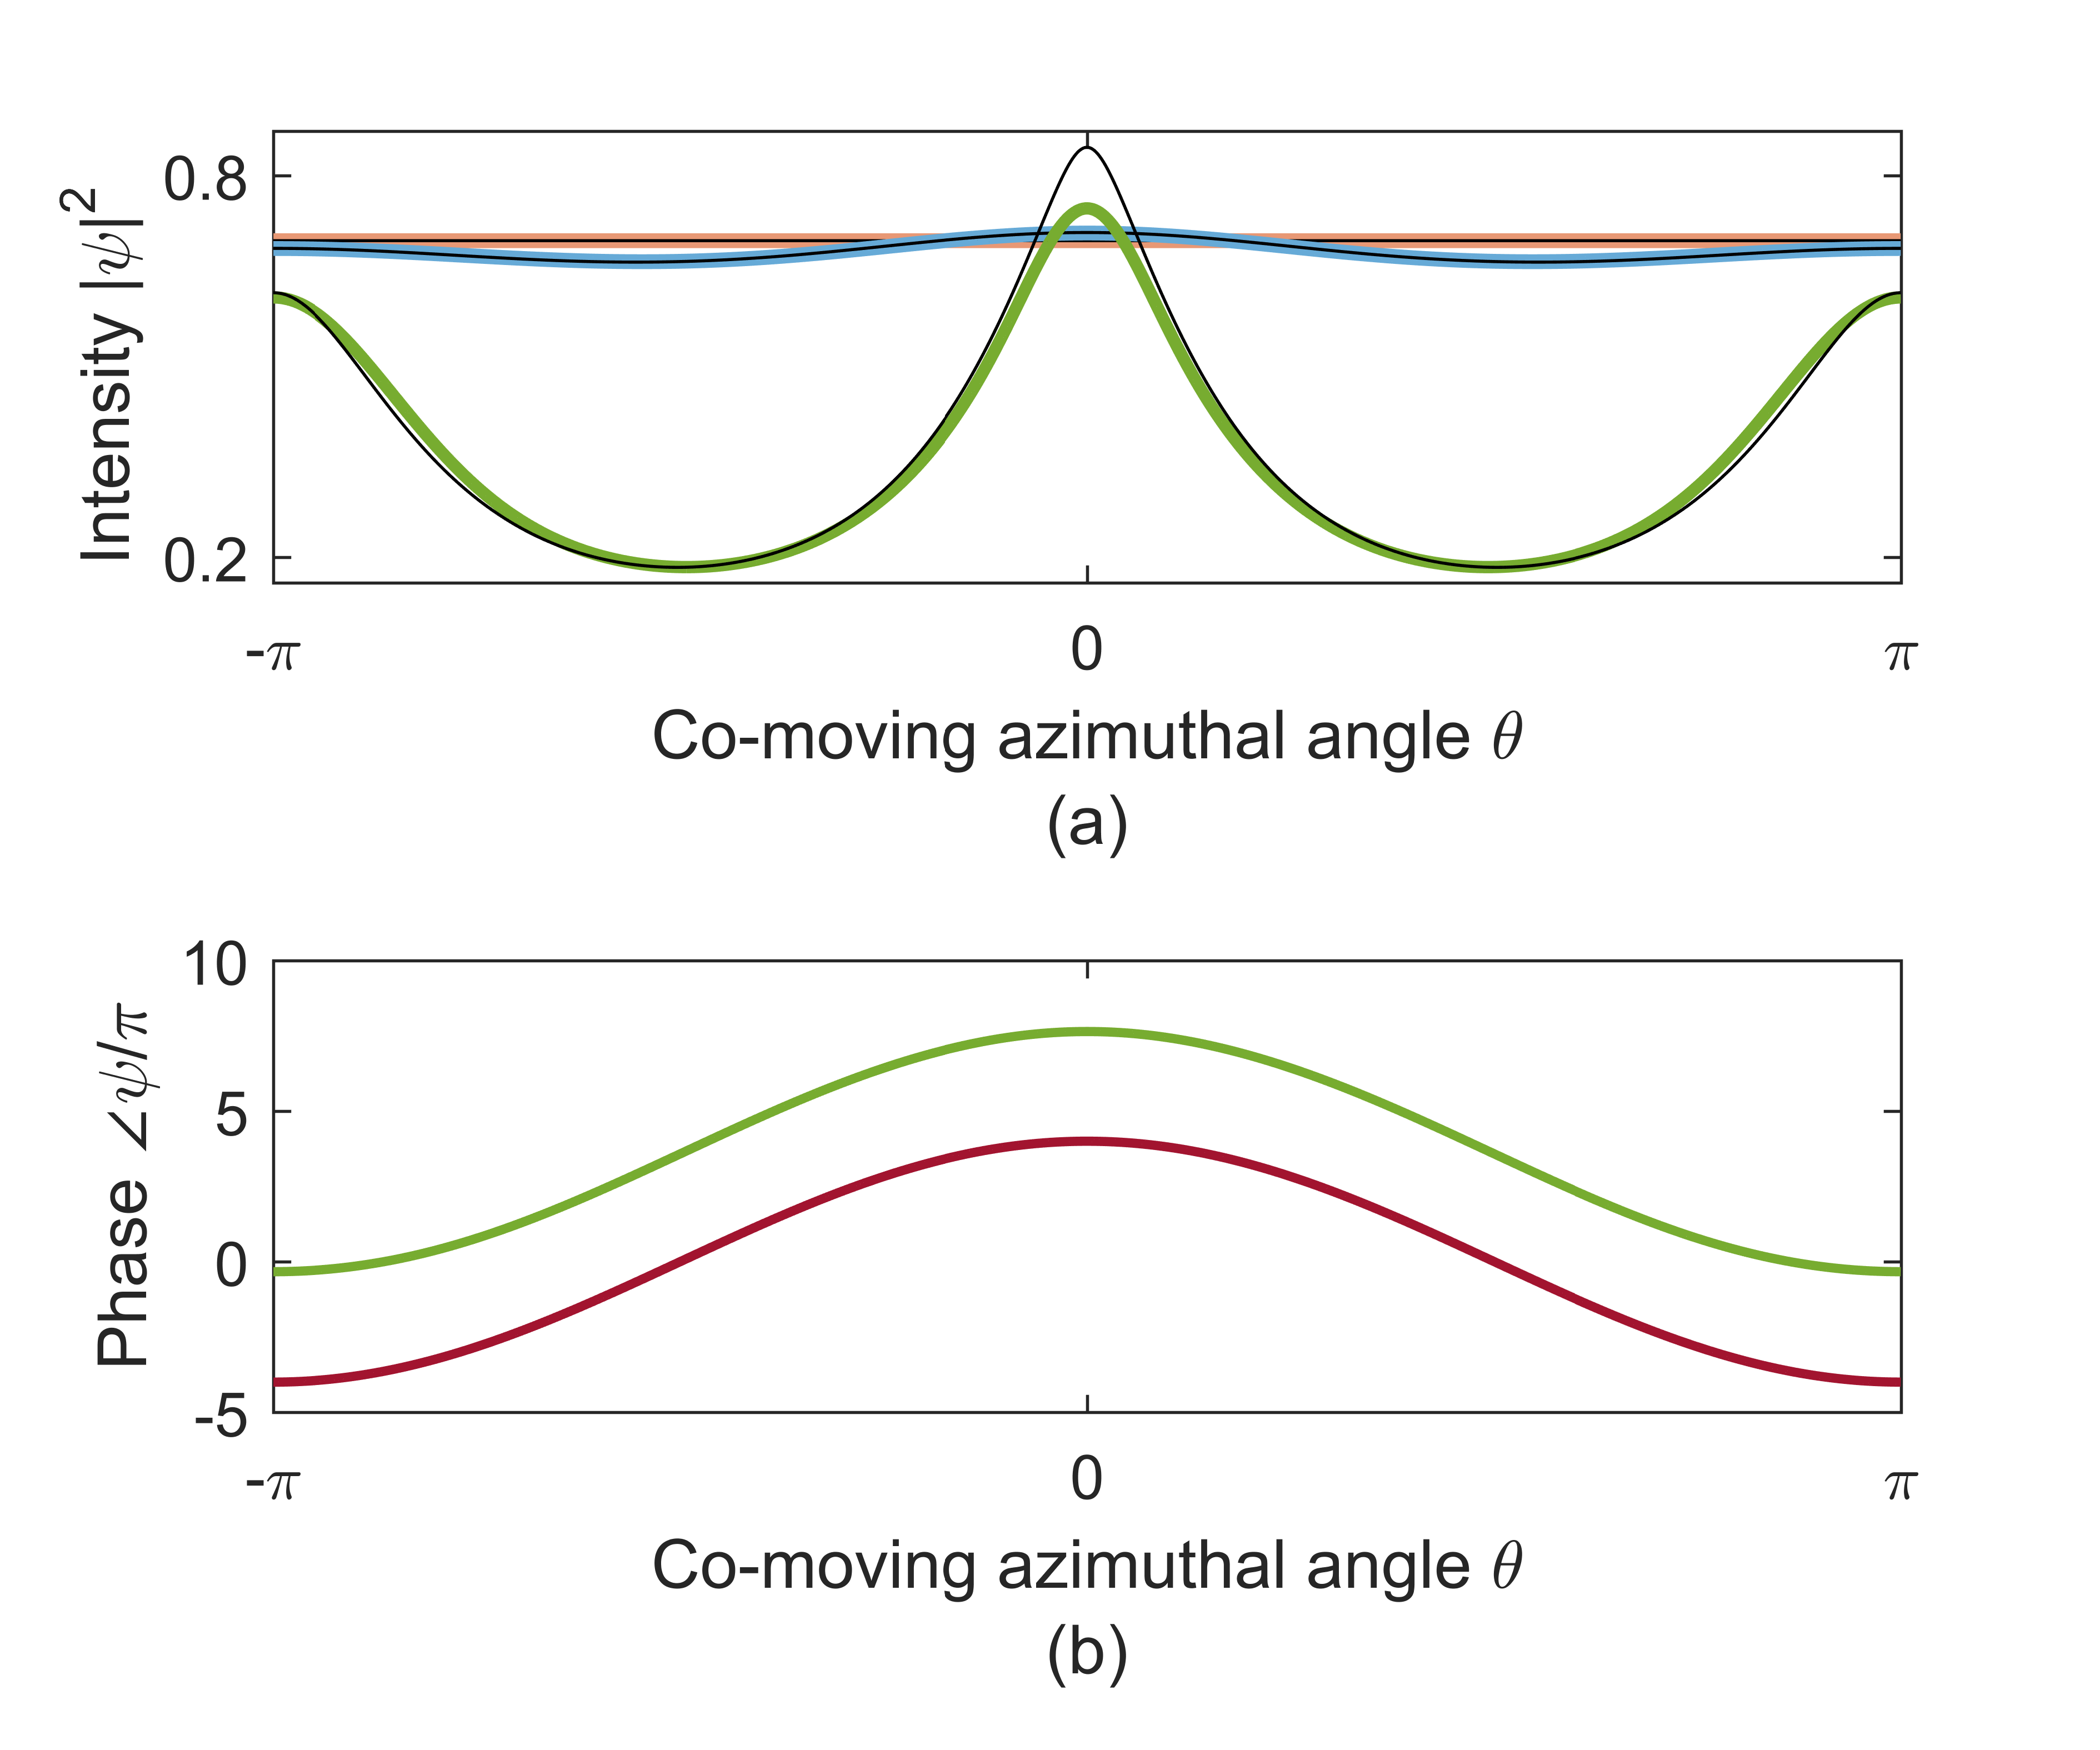
\includegraphics{\FigPath/Figures/PMPumping/PM_background.png}
	\end{center}
	\caption[Quasi-CW background in a PM-pumped resonator]{\textbf{Quasi-CW background in a PM-pumped resonator.} (a) Simulated intensity of the background in the resonator without (orange) and with PM of depth $\delta_{PM}=\pi/2$ (blue) and $\delta_{PM}=4\pi$ (green), with analytical approximations in black. Here $\alpha$ is slightly larger than the critical value for soliton formation. (b) Phase profile of the field $\psi$ corresponding to the green trace in (a) with $\delta_{PM}=4\pi$, and the phase profile of the driving term $Fe^{i\delta_{PM}\cos{\theta}}$ (red) with modulation depth $4\pi$. The phase of the field is very nearly the phase of the drive plus a constant offset.}
	\label{fig:PMbackground}
\end{figure} 

Fig. \ref{fig:PMbackground} shows the predictions of simulations of Eq. \ref{eq:PMLLE} (color) and the analytical model Eq. \ref{eq:PMLLEstat2} (black). The two agree quantitatively for weak modulation ($\delta_{PM}=\pi/2$, blue) and qualitatively with larger depth ($\delta_{PM}=4\pi$, green); both indicate that the field $\psi$ exhibits amplitude variations due to the spatially-varying effective loss and detuning. This phenomenon suggests an explanation for the spontaneous formation of a single soliton as the detuning $\alpha$ is decreased in terms of the local disappearance of Kerr bistability.

As discussed in Sec. \ref{sec:MRanalyticalcurves}, for the LLE with a CW pump the background field $\psi_s$ can take one of two stable values over a range of the parameters $\alpha$ and $F^2$. This leads to the emergence of a tilted resonance lineshape like the one shown in Fig. \ref{fig:PMalphacrit}a, with an effectively red-detuned branch lying at higher values of $\alpha$, an effectively blue-detuned branch lying at lower values of $\alpha$, and an interval in $\alpha$ over which they both exist and the system is bistable (recall that the middle branch is unstable). With spatially-varying effective loss and detuning terms, the field $\psi_s(\theta)$ described by Eq. \ref{eq:PMLLEstatpsi} now takes a value at each point in the cavity that is determined by the local parameters $\gamma(\theta)$ and $\eta(\theta)$, with the result that each point lies on its own effective resonance. The resulting resonance \textit{surface} is shown in Fig. \ref{fig:PMalphacrit}b. It can be independently determined for each point in the cavity whether $\psi_s(\theta)$ exhibits bistability. Applying the analysis presented in Sec. \ref{sec:MRanalyticalcurves} to Eq. \ref{eq:PMLLEstat2}, we identify the value of $\rho$ associated with the disappearance of the bistability in a decreasing-$\alpha$ scan as the smaller value $\rho_-$ at which $\partial F^2/\partial\rho=0$:
\begin{equation}
\rho_-=\left(2\eta-\sqrt{\eta^2-3\gamma^2}\right)/3,
\end{equation}
For fixed $F^2$ the function $\alpha_{crit}(\theta)$ describing the critical value of $\alpha$ at which the bistability ends is found by numerically solving the implicit equation for $\alpha_{crit}$ obtained by inserting $\rho_-$ into Eq. \ref{eq:PMLLEstat}:
\begin{equation}
F^2=\left[\gamma^2(\theta)+\left(\eta(\theta)-\rho_-(\theta)\right)^2\right]\rho_-(\theta),
\end{equation}
where $\alpha_{crit}(\theta)$ is included via $\eta(\theta)=\alpha_{crit}(\theta)-\frac{\beta_2}{2}\delta_{PM}^2\sin^2{\theta}$. Fig. \ref{fig:PMalphacrit}c shows a calculation of $\alpha_{crit}(\theta)$ for $F^2=4$ and $\beta_2=-0.0187$, which is chosen to match the dispersion of the resonator used for the experiments presented below. For $\theta=0$ this calculation predicts disappearance of the bistability, and subsequent soliton generation, at $\alpha=2.741$, which is a difference of 0.4 \% from the value $\alpha=2.729$ observed in the simulation presented in Fig. \ref{fig:PMenergylevels}. The same calculation predicts disappearance of the bistability for $\theta=\pi$ at $\alpha=2.705$, also in close agreement with the simulation.



%\begin{figure}[htpb]
%	\begin{center}
%		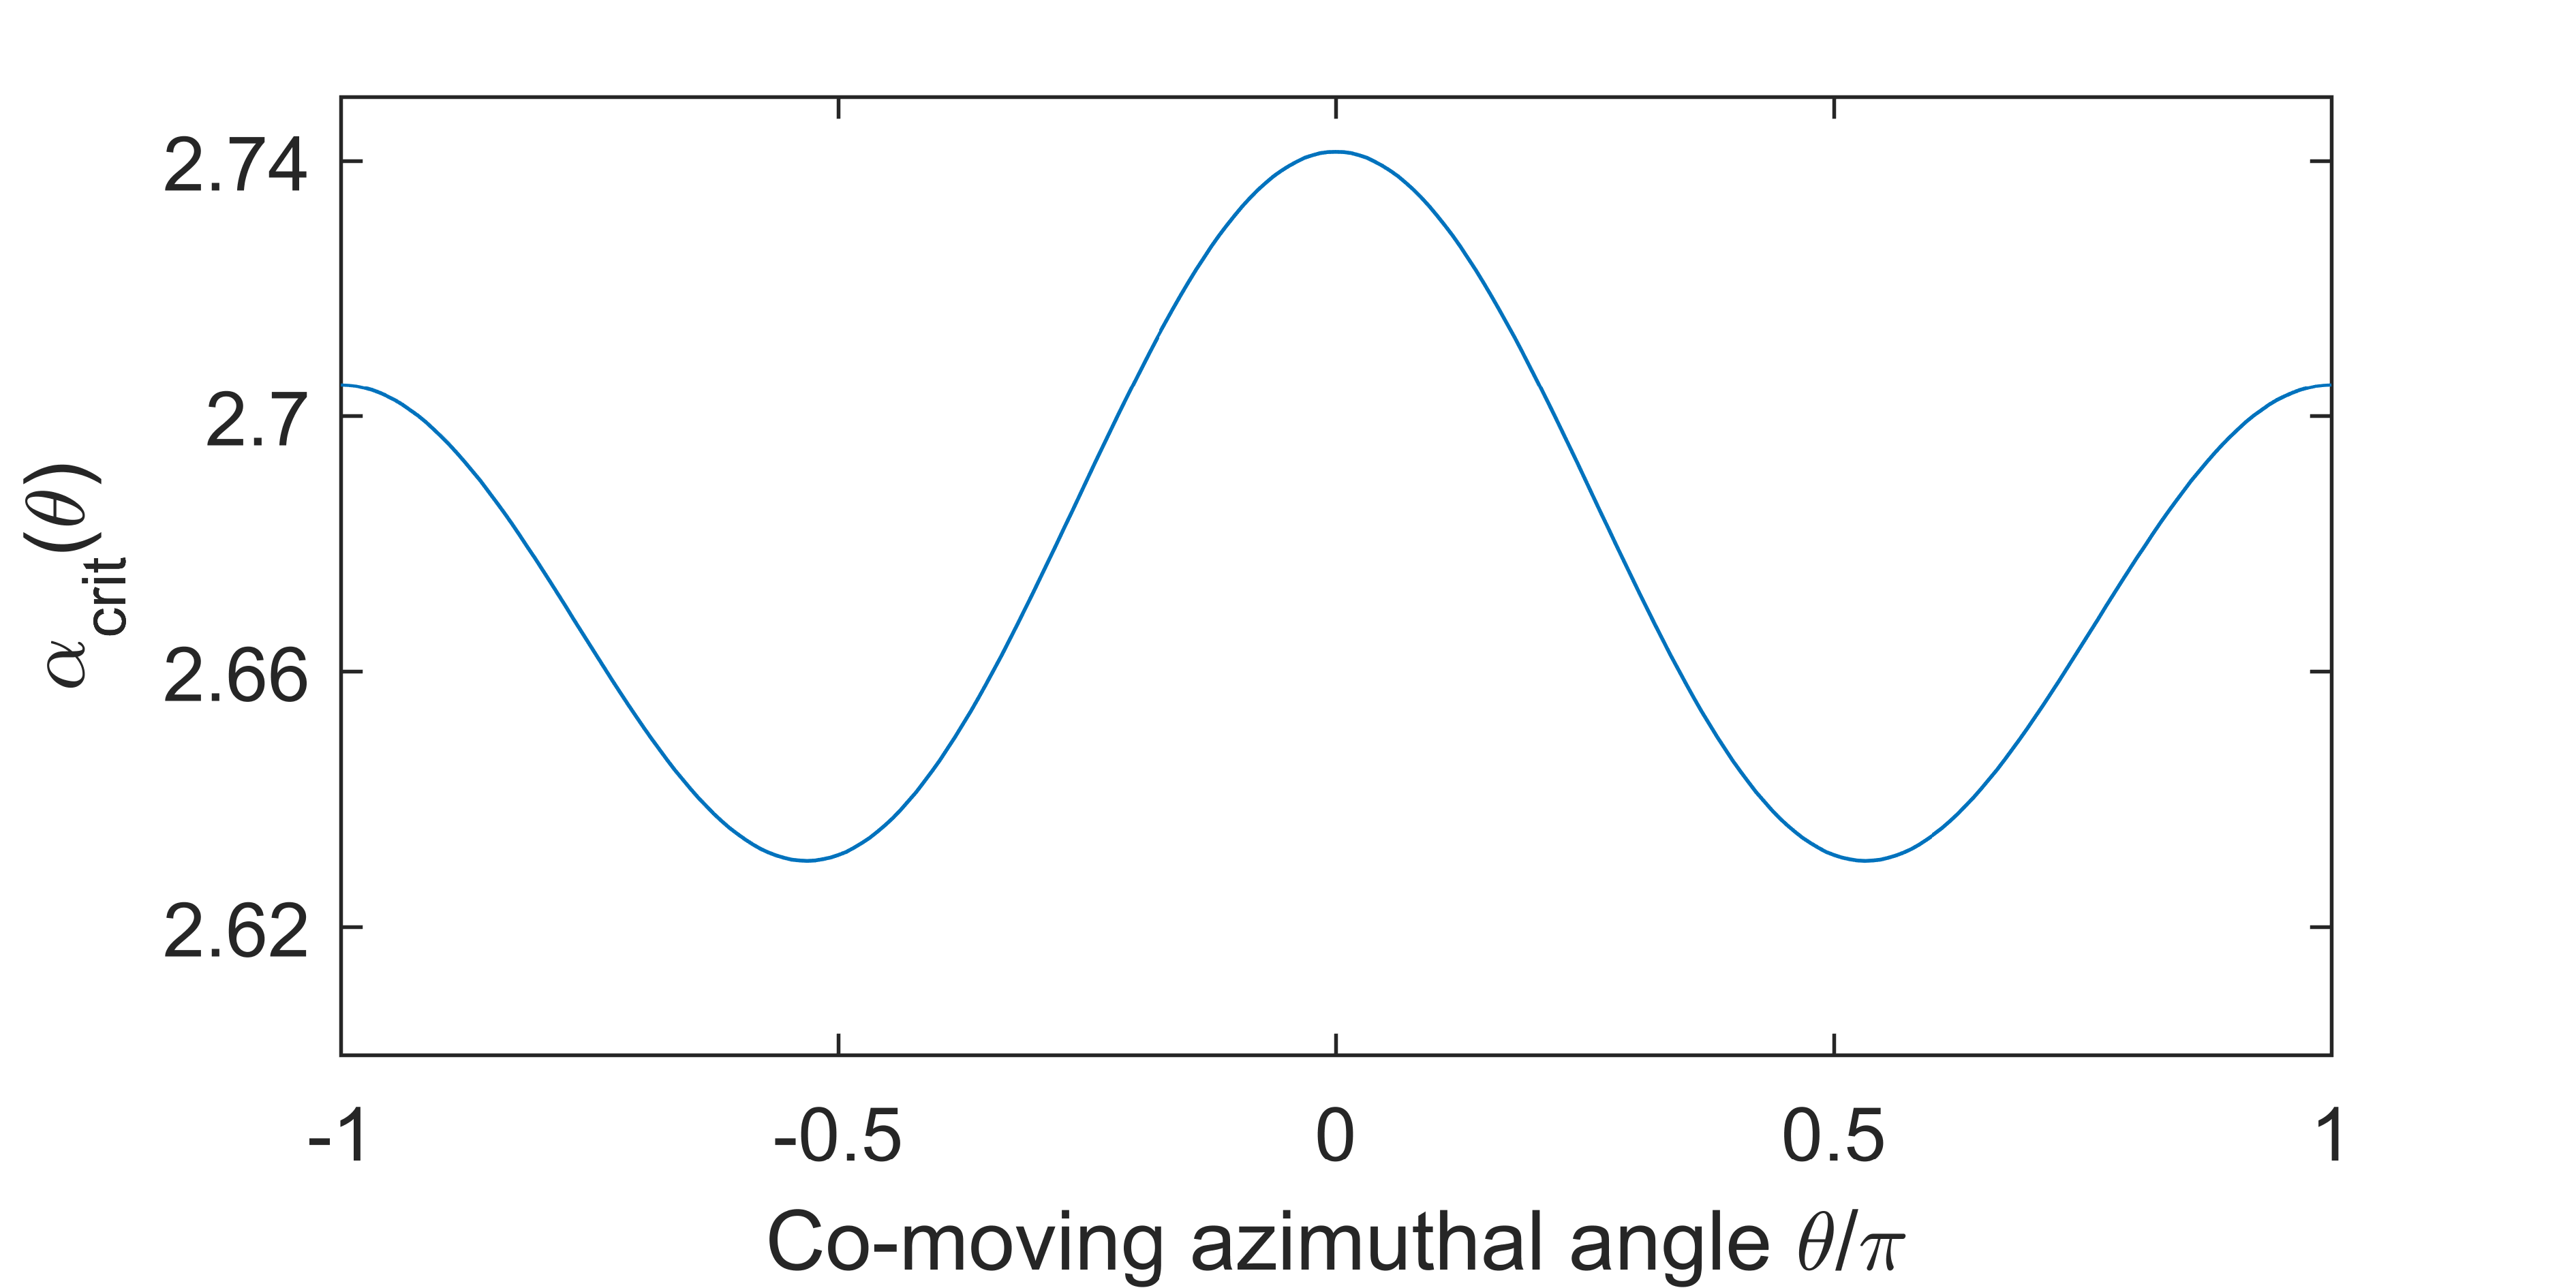
\includegraphics{\FigPath/Figures/PMPumping/PMalphacrit.png}
%	\end{center}
%	\caption[Critical values of $\alpha$ for the disappearance of Kerr bistability]{\textbf{Critical values of $\alpha$ for the disappearance of Kerr bistability.} A plot of the value $\alpha_{crit}(\theta)$ at which the Kerr bistability vanishes \textit{locally} and the system must locally jump to the effectively blue-detuned branch. This plot is generated with $F^2=$, $\beta=-0.0187$. The value $\alpha_{crit}(\theta=0)$ can be used to approximate the detuning at which a soliton is generated in an increasing-frequency scan of the pump laser.}
%	\label{fig:PMalphacrit}
%\end{figure} 

%\begin{figure}[htpb]
%	\begin{center}
%		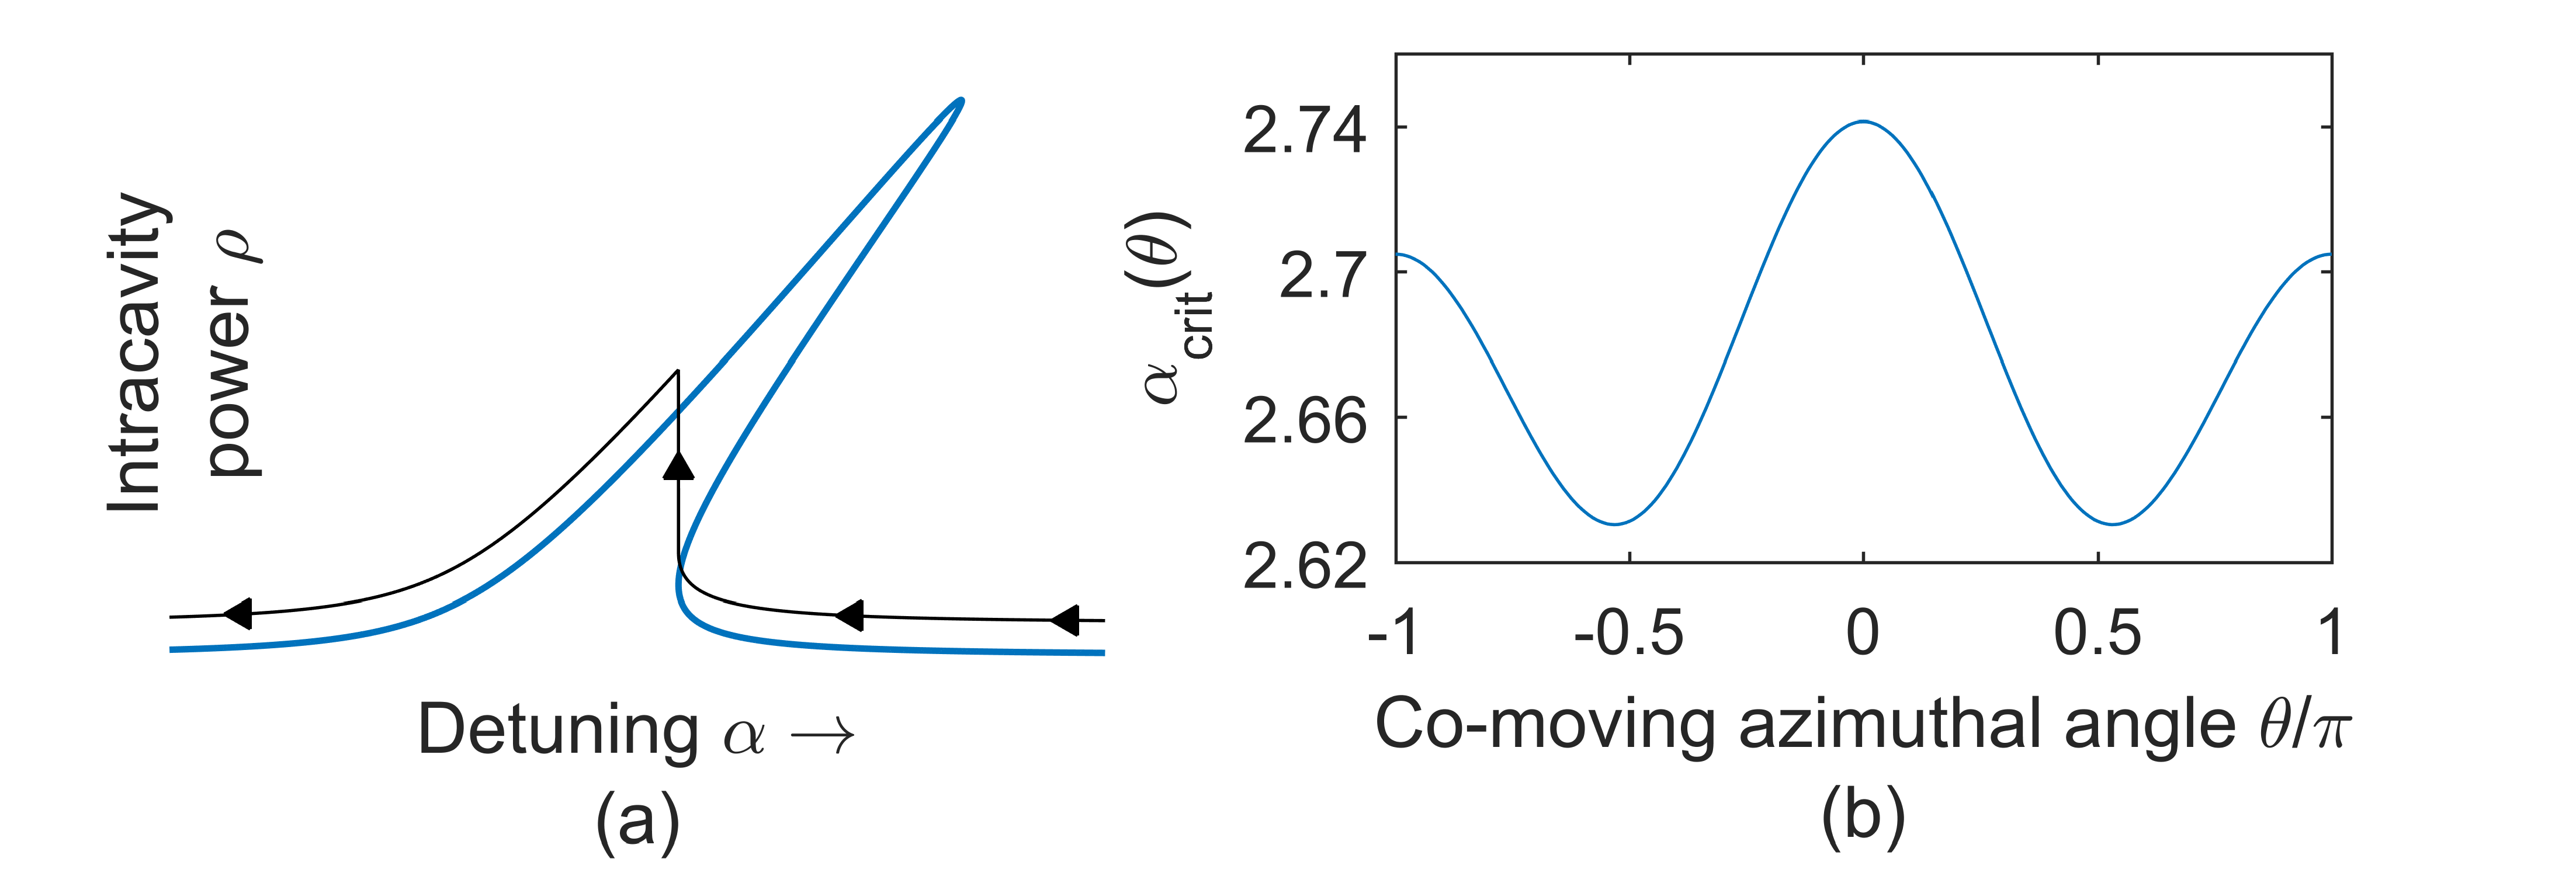
\includegraphics{\FigPath/Figures/PMPumping/PMalphacritWres.png}
%	\end{center}
%	\caption[Mechanism for soliton generation with a PM pump]{\textbf{Mechanism for soliton generation with a PM pump.} (a) Plot of a Kerr-shifted resonance, here with $F^2$=12. The CW background field $\psi$ follows the black curve in an increasing-frequency scan of the pump laser. For the case of a phase-modulated pump, the field $\psi_s(\theta)$ lies at a point on a qualitatively similar resonance that is defined locally by $\gamma(\theta)$ and $\eta(\theta$) for each point $\theta$ in the co-moving frame. (b) A plot of the value $\alpha_{crit}(\theta)$ at which the Kerr bistability locally vanishes and the field $\psi_s(\theta)$ must jump to the effectively blue-detuned branch, associated with the vertical transition in (a). This plot is generated with $F^2=4$, $\beta=-0.0187$. The value $\alpha_{crit}(\theta=0)$ can be used to approximate the detuning at which a soliton is generated in an increasing-frequency scan of the pump laser.}
%	\label{fig:PMalphacrit}
%\end{figure} 

\begin{figure}[htpb]
	\begin{center}
		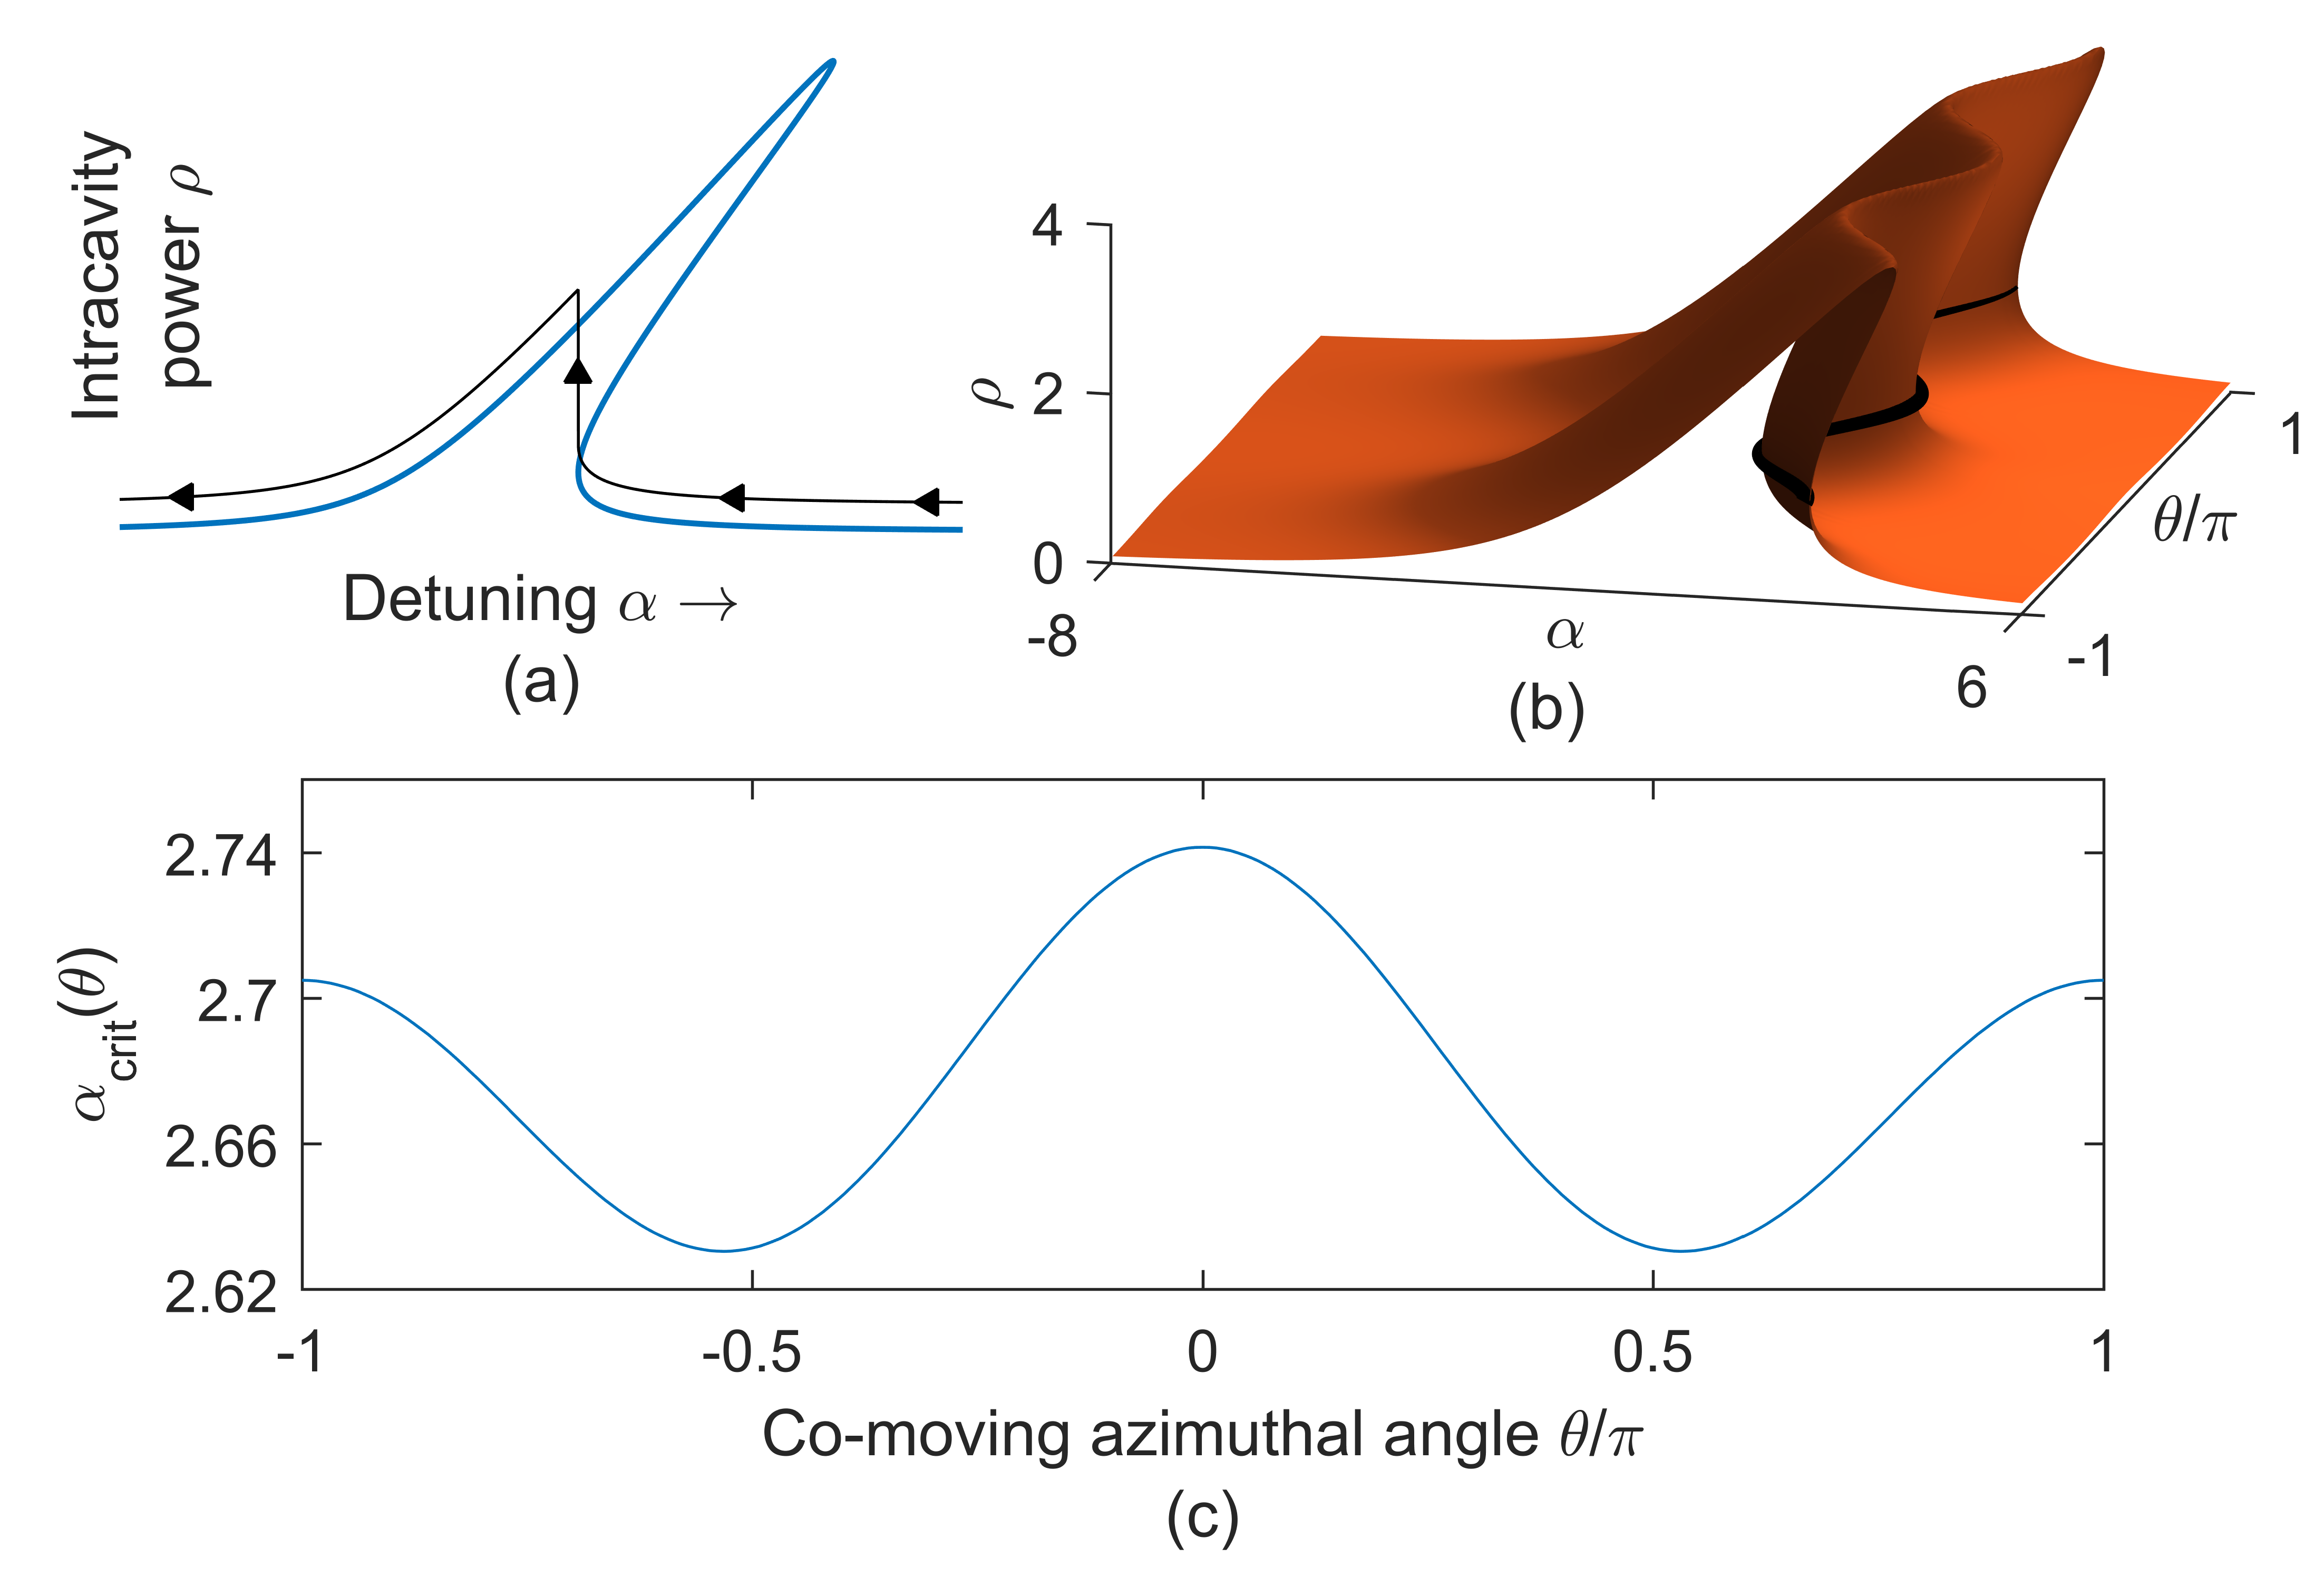
\includegraphics{\FigPath/Figures/PMPumping/PMalphacritWresWmanifold.png}
	\end{center}
	\caption[Mechanism for soliton generation with a PM pump]{\textbf{Mechanism for soliton generation with a PM pump.} (a) Plot of a Kerr-shifted resonance, here with $F^2$=12. The CW background field $\psi$ follows the black curve in an increasing-frequency scan of the pump laser. (b) For the case of a phase-modulated pump, the field $\psi_s(\theta)$ at each point $\theta$ lies on a qualitatively similar resonance that is defined locally by $\gamma(\theta)$ and $\eta(\theta$), with the result that a resonance surface emerges. The resonance surface is shown here for $F^2=4$, $\beta_2=-0.0187$, and $d_{PM}=4\pi$, which is chosen to accentuate the $\theta$-dependence. The curve $\alpha_{crit}(\theta)$ is shown in black. (c) A plot of the value $\alpha_{crit}(\theta)$ at which the Kerr bistability locally vanishes and the field $\psi_s(\theta)$ must jump to the effectively blue-detuned branch, associated with the vertical transition in (a), for $F^2=4$, $\beta_2=-0.0187$, and $\delta_{PM}=\pi$. The value $\alpha_{crit}(\theta=0)$ can be used to approximate the detuning at which a soliton is generated in an increasing-frequency scan of the pump laser; the input parameters here match the level diagram in Fig. \ref{fig:PMenergylevels}.}
	\label{fig:PMalphacrit}
\end{figure} 

%These parameters determine whether the quasi-CW background locally exhibits the bistability that is well-known in the case of a CW pump laser [18,21], which suggests a mechanism for spontaneous single-soliton generation: as α is decreased, the stable effectively red-detuned branch of the resonance locally vanishes at the peak of the quasi-CW background, leading to the formation of a soliton. By following the analysis in e.g. Ref.  [18] (Eqs. 11-14), we can approximate the value of α where this occurs at θ=0; for the diagram shown in Fig. 1b this predicts soliton generation at α=2.741, in excellent agreement (0.4 % error) with the value α=2.729 obtained in numerical simulations. 
%
%Fig.  compares the predictions of numerical LLE simulations (color) with the analytical model (black). The two agree quantitatively at small modulation depth () and qualitatively at larger depth . Both the simulations and the approximate analytical solution indicate that the background has two peaks per round trip in the presence of phase modulation, which suggests a mechanism for spontaneous single-soliton generation: \todo{update this} At threshold the larger peak becomes locally unstable, and a soliton is formed by local modulation instability \cite{Ceoldo2016,Wang2018}. Moreover, it is known that if solitons exist elsewhere they are pushed to the larger peak by the background’s modulated phase \cite{Jang2015a}. This makes superpositions of $N>1$ solitons unstable and practically forbidden. Generation of single solitons then simply requires tuning the pump power and frequency to appropriate values, regardless of initial conditions. 
%
%The detuning for soliton generation can be estimated using Eq. \ref{eq:PMLLEstat} by calculating the value of $\alpha$ where $\rho(\theta=0)=1$. This comes with a further approximation, as simulations reveal that the critical detuning for soliton formation is near but not necessarily at $\rho=1$ because the spatial interval over which threshold is exceeded must have some minimum width. However, this approach quantitatively captures the behavior shown in Fig. \ref{fig:PMenergylevels}, predicting soliton generation at $\alpha=2.737$.

\section{Spontaneous generation of single solitons using a phase-modulated pump laser}


We demonstrate deterministic generation of single solitons without condensation from an extended pattern in a 22-GHz FSR silica micro-disk resonator with $\Delta\nu\sim$ 1.5 MHz linewidth \cite{Lee2012}. We generate a frequency-agile laser for pumping the resonator by passing a CW seed laser through a single-sideband modulator (SSB) that is driven by a voltage-controlled oscillator (VCO) \cite{Stone2017}. The seed laser is extinguished in the modulator and the resulting sideband can be swept by adjusting the voltage applied to the VCO; sweeping rates up to 100 GHz/$\mathrm{\mu}$s over a range over 4 GHz are possible. The pump laser is phase-modulated with index $\delta_{PM}\sim\pi$ and amplified to normalized power $F^2$ between 2 and 6. We are able to measure the pump-laser detuning in real time using an AOM-shifted probe beam as shown in Fig. \ref{fig:PMsetup}, and the high-bandwidth feedback allowed by the VCO/SSB scheme allows thermal instabilities associated with the red detuning that is required for soliton generation to be overcome. 

\begin{figure}[htpb]
	\begin{center}
		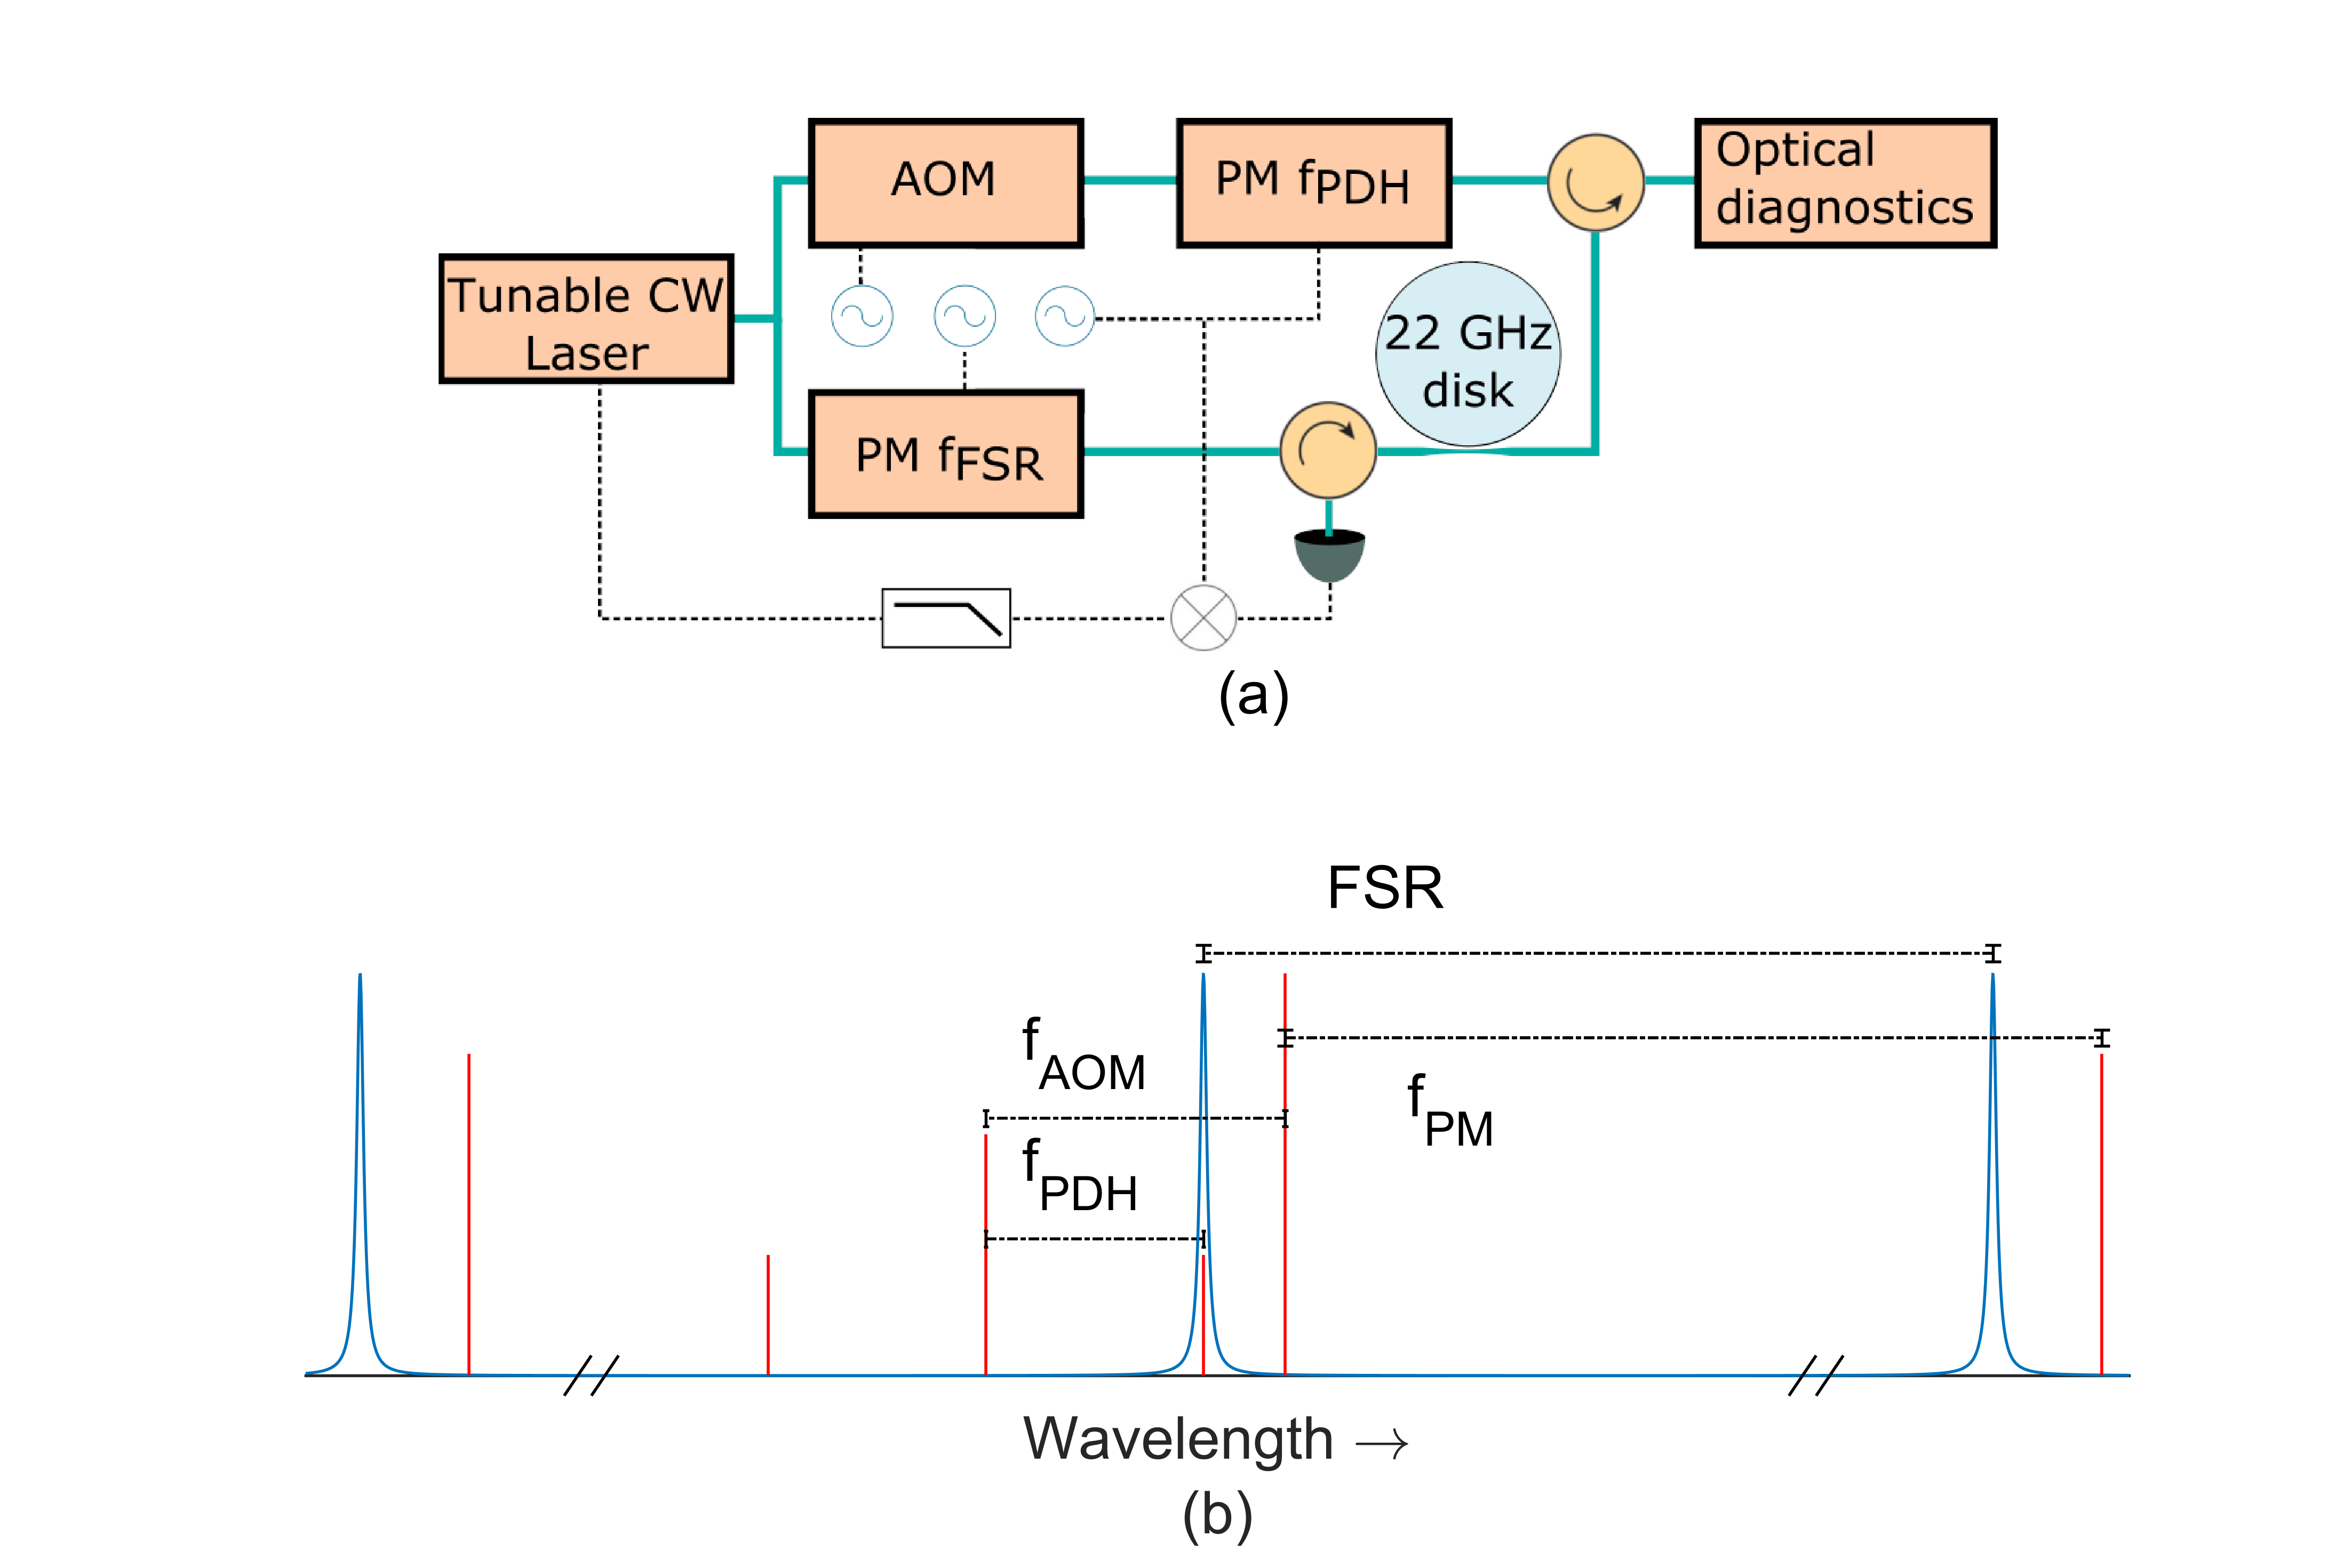
\includegraphics{\FigPath/Figures/PMPumping/PMsetup.png}
	\end{center}
	\caption[Experimental setup for soliton generation with a phase-modulated pump laser]{\textbf{Experimental setup for soliton generation with a phase-modulated pump laser.} (a) Schematic diagram of the experimental setup, including the pump laser phase-modulated at frequency $f_{PM}\sim f_{FSR}$ and an AOM-shifted probe beam that is modulated at frequency $f_{PDH}$ for implementation of a Pound-Drever-Hall sideband lock. The probe beam addresses the resonator in the counter-propagating direction. (b) Frequency-domain diagram of the scheme used to maintain stable red detuning of the pump laser. As $f_{PDH}$ is increased, the detuning $\alpha$ is decreased.}
	\label{fig:PMsetup}
\end{figure} 


To generate single solitons, we begin with large red detuning $\nu_0-\nu_{pump}=$40 MHz and decrease the detuning until a soliton is generated near $\nu_0-\nu_{pump}\sim$5 MHz detuning; this value depends on the pump power and coupling condition. We measure the power converted by the Kerr nonlinearity to new frequencies by passing a portion of the resonator's output through an optical band-reject filter; this `comb power' measurement reveals a step upon soliton formation, as shown in Fig. \ref{fig:PMgen}a, after which we can measure the soliton spectrum with phase-modulation sidebands on the pump shown in Fig. \ref{fig:PMgen}b. After soliton generation, we observe that the soliton can be preserved while the detuning is increased again, consistent with Fig. \ref{fig:PMenergylevels}. Additionally, we observe that it is possible to turn off the phase modulation without loss of the soliton, in agreement with the simulations presented in Ref. \cite{Taheri2015}.

Automating soliton generation by repeatedly scanning the laser into resonance ($\nu_0-\nu_{pump}\sim$5 MHz) and back out again ($\nu_0-\nu_{pump}\sim$20 MHz, far enough that the soliton is lost) has enabled reversible generation of 1000 solitons in 1000 trials over 100 seconds, with a measured 100 $\%$ success rate. Our probe beam allows measurement of the detuning at which soliton generation occurs, which changes little from run to run. We present a histogram of detuning measurements for the generation of 160 solitons in Fig. \ref{fig:PMgen}c. 

\begin{figure}[htpb]
	\begin{center}
		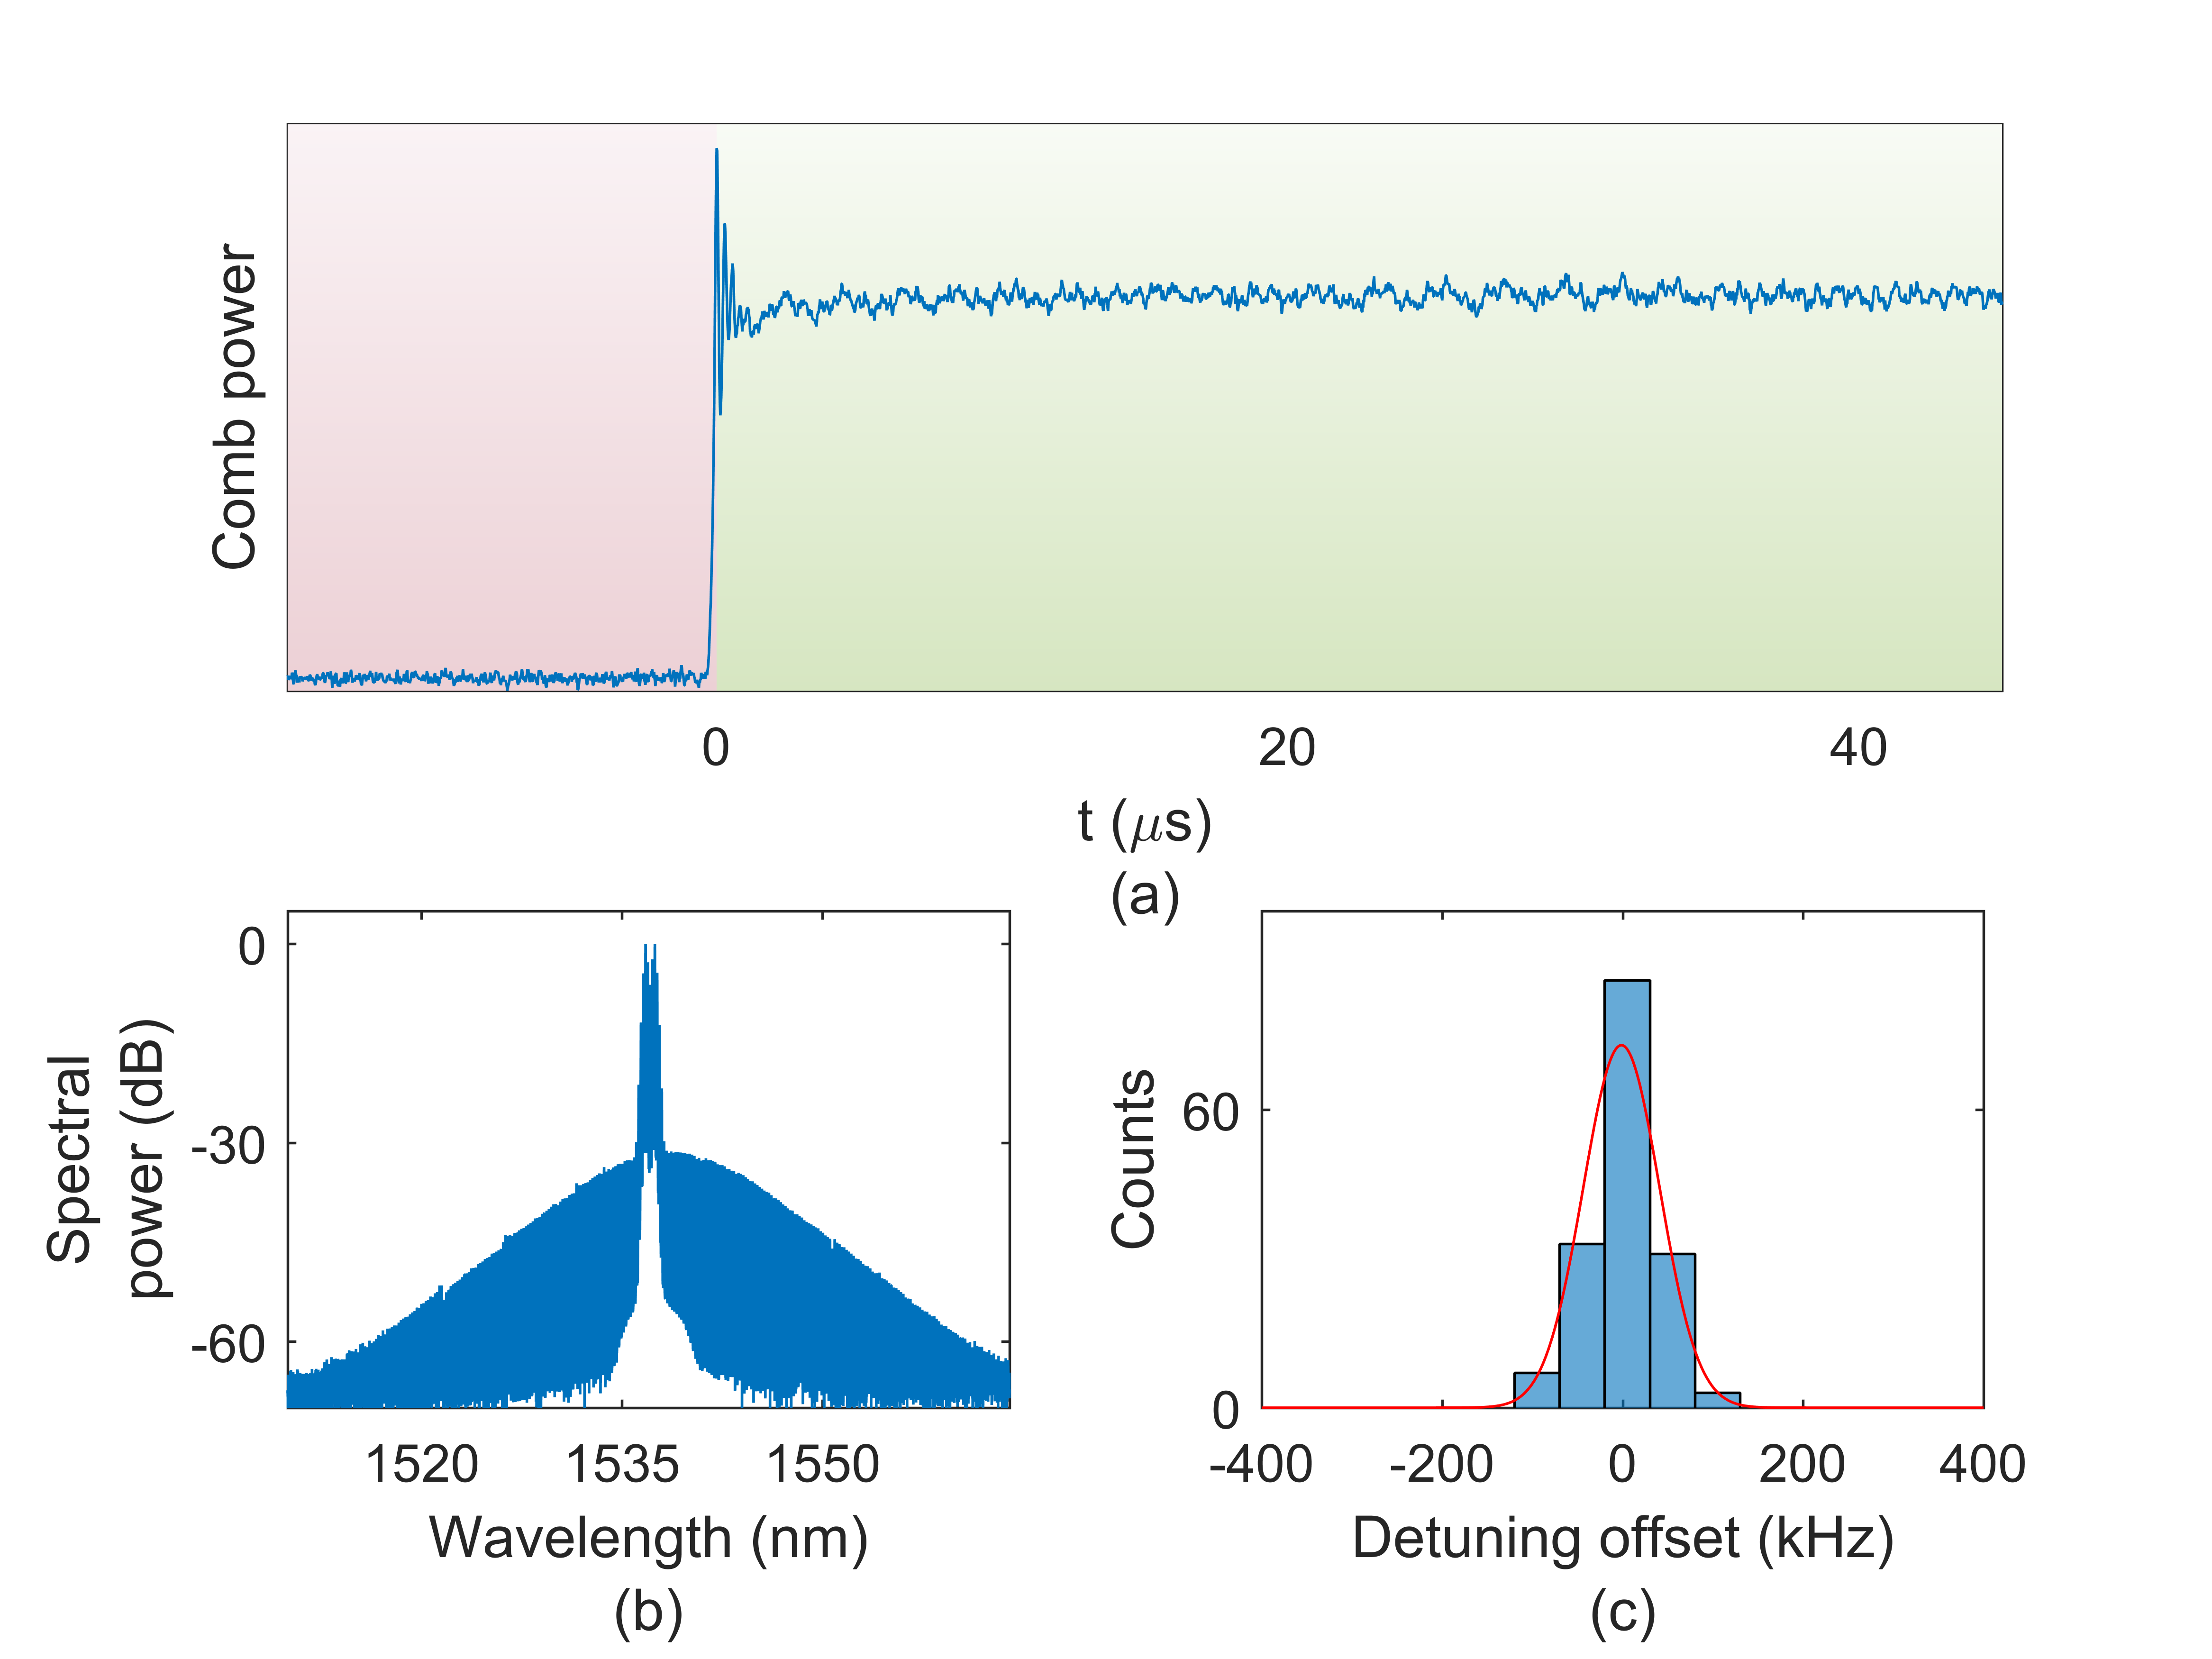
\includegraphics{\FigPath/Figures/PMPumping/PMstepAndSpecAndHist.png}
	\end{center}
	\caption[Spontaneous generation of solitons using a phase-modulated pump laser]{\textbf{Spontaneous generation of solitons using a phase-modulated pump laser.} (a)~`Comb power' trace obtained by filtering the pump laser out of the spectrum of light transmitted past the resonator, indicating a discrete step in the amount of frequency-converted light upon direct generation of a soliton. (b) Optical spectrum of a spontaneously generated soliton. The spectrum of the phase-modulated pump laser is visible as the set of higher-amplitude lines in the center. (c)~Histogram of measured detuning values at which a soliton is generated relative to a reference (mean) value over 160 trials.}
	\label{fig:PMgen}
\end{figure} 

\section{Soliton control using a phase-modulated pump laser}

In addition to enabling deterministic generation of single solitons, phase modulation of the pump laser also facilitates timing and repetition-rate control of the resulting pulse train. We characterize this control by measuring the repetition rate of the soliton pulse train as the phase-modulation frequency is varied. This measurement is conducted as follows: First, we photodetect the pulse train after removing the central spectral lines corresponding to the phase-modulated pump laser using an optical band-reject filter. Then, in order to obtain a measurement trace of the repetition rate as a function of time, the photodetected signal is mixed with a local oscillator to reduce the signal frequency to $\sim$ 1 MHz, after which a spectrogram of the resulting waveform is calculated.



Fig. \ref{fig:PMsweep} shows the measured repetition rate $f_{rep}$ as $f_{PM}$ is swept sinusoidally through a range of $\pm$50 kHz around the soliton's natural repetition rate; the repetition rate follows the PM except for glitches near the peaks of the sweep when $f_{PM}-f_{rep}$ exceeds a locking bandwidth of about $\pm$40 kHz. This observation is consistent with an estimate of the locking range $\delta_{PM}\times D_2/2\pi\sim$44 kHz that is presented in Ref. \cite{Jang2015a}, where we have used the approximate value $D_2=$14 kHz/mode ($\beta_2=-2D_2/\Delta\omega_{tot}=-0.0187$, via $\Delta\nu\sim$1.5 MHz). In the inset of Fig. \ref{fig:PMsweep} we overlay the results of LLE simulations that qualitatively match the observed behavior. These simulations are conducted by introducing the term $+\beta_1\frac{\partial\psi}{\partial\theta}$ to the right-hand side of Eq. \ref{eq:PMLLE}, where $\beta_1=-2(f_{FSR}-f_{PM})/\Delta\nu$ incorporates a difference between the modulation frequency and the FSR of the resonator into the model; $\beta_1$ may be varied in time to simulate the sweep of $f_{PM}$. These simulations indicate that the periodic nature of the glitches is due to the residual pulling of the phase modulation on the soliton when the latter periodically cycles through the pump's phase maximum.

\begin{figure}[htpb]
	\begin{center}
		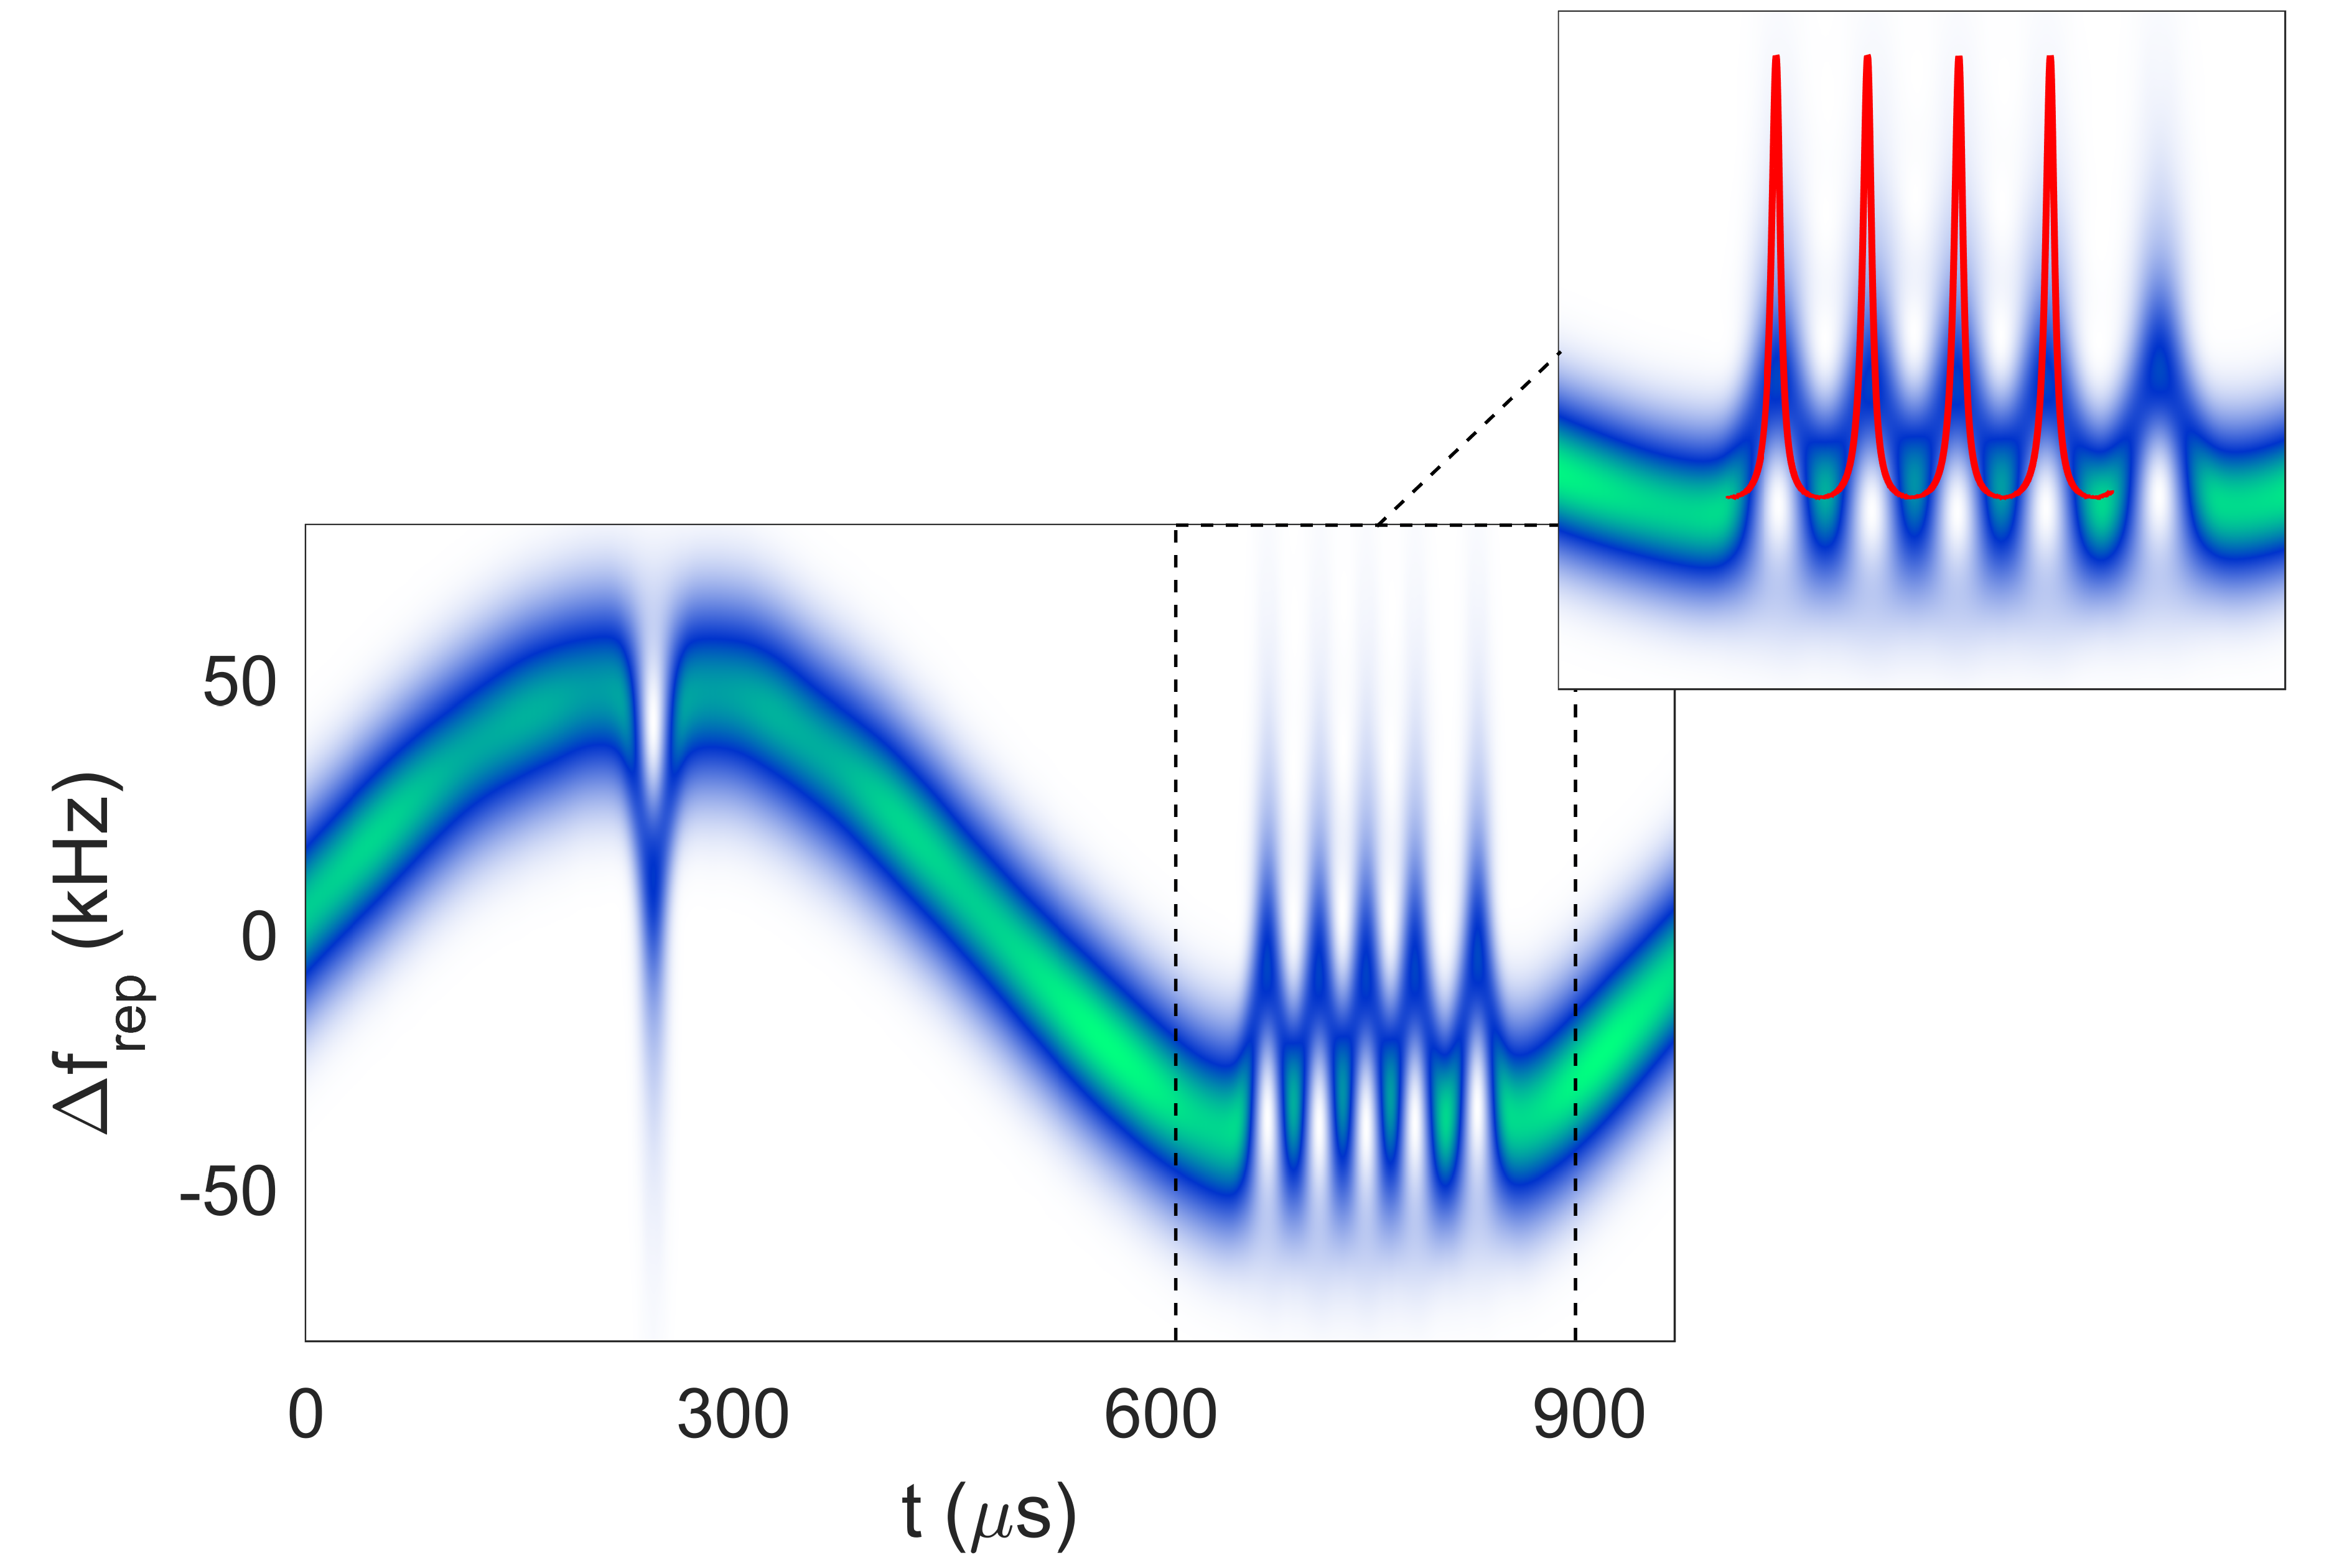
\includegraphics{\FigPath/Figures/PMPumping/PMsweep.png}
	\end{center}
	\caption[Repetition-rate control using a phase-modulated pump laser]{\textbf{Repetition-rate control using a phase-modulated pump laser.} Spectrogram of the measured repetition rate of the soliton pulse train generated by a phase-modulated pump laser as the frequency of phase modulation is swept through $\pm$50 kHz over 1 ms. Glitches in the spectrogram indicate that the range over which $f_{rep}$ can be locked to $f_{PM}$ has been exceeded. Inset: Qualitative agreement with simulations when $f_{PM}$ is outside of the locking bandwidth, shown in red. As the soliton and the pump phase evolve at different frequencies $f_{rep}$ and $f_{PM}$, the soliton periodically approaches the maximum of the phase profile. The soliton's group velocity changes, nearly locking to the phase modulation, before becoming clearly unlocked again.}
	\label{fig:PMsweep}
\end{figure} 


To evaluate the utility of phase modulation for fast control of the soliton's properties, we measure the repetition rate of the pulse train as $f_{PM}$ is rapidly switched by $\pm$40 kHz, which is within the soliton's locking range.  To measure these fast dynamics, we split the photodetected repetition-rate signal and send one path through a reactive circuit element (a set of low-pass filters) that induces a frequency-dependent phase shift. By comparing the phase between the two paths as a function of time, the time-dependent repetition rate can be determined. We construct eye-diagrams out of the resulting data; these are shown in Fig. \ref{fig:PMeyediags}. In Fig. \ref{fig:PMeyediags}a, $f_{PM}$ is switched with 200 $\mu$s period and 10 $\mu$s transition time; in Fig. \ref{fig:PMeyediags}b it is switched with 100 $\mu$s period and 60 ns transition time. These eye diagrams show that the PM enables exquisite control of the soliton pulse train.

We overlay a simulated eye diagram on the data in Fig. \ref{fig:PMeyediags}b. This simulation is conducted for parameters $\Delta\nu=1.5$ MHz, $\delta_{PM}=0.9\pi$ that are near the experimental values, and the agreement between measurement and simulation indicates that the measurements are consistent with fundamental LLE dynamics. Fig. \ref{fig:PMeyediags}c presents the results of additional LLE simulations; the basic result is that the switching speed of $f_{rep}$ is limited by the resonator linewidth, and can be only modestly improved by increasing $\delta_{PM}$. 

\begin{figure}[htpb]
	\begin{center}
		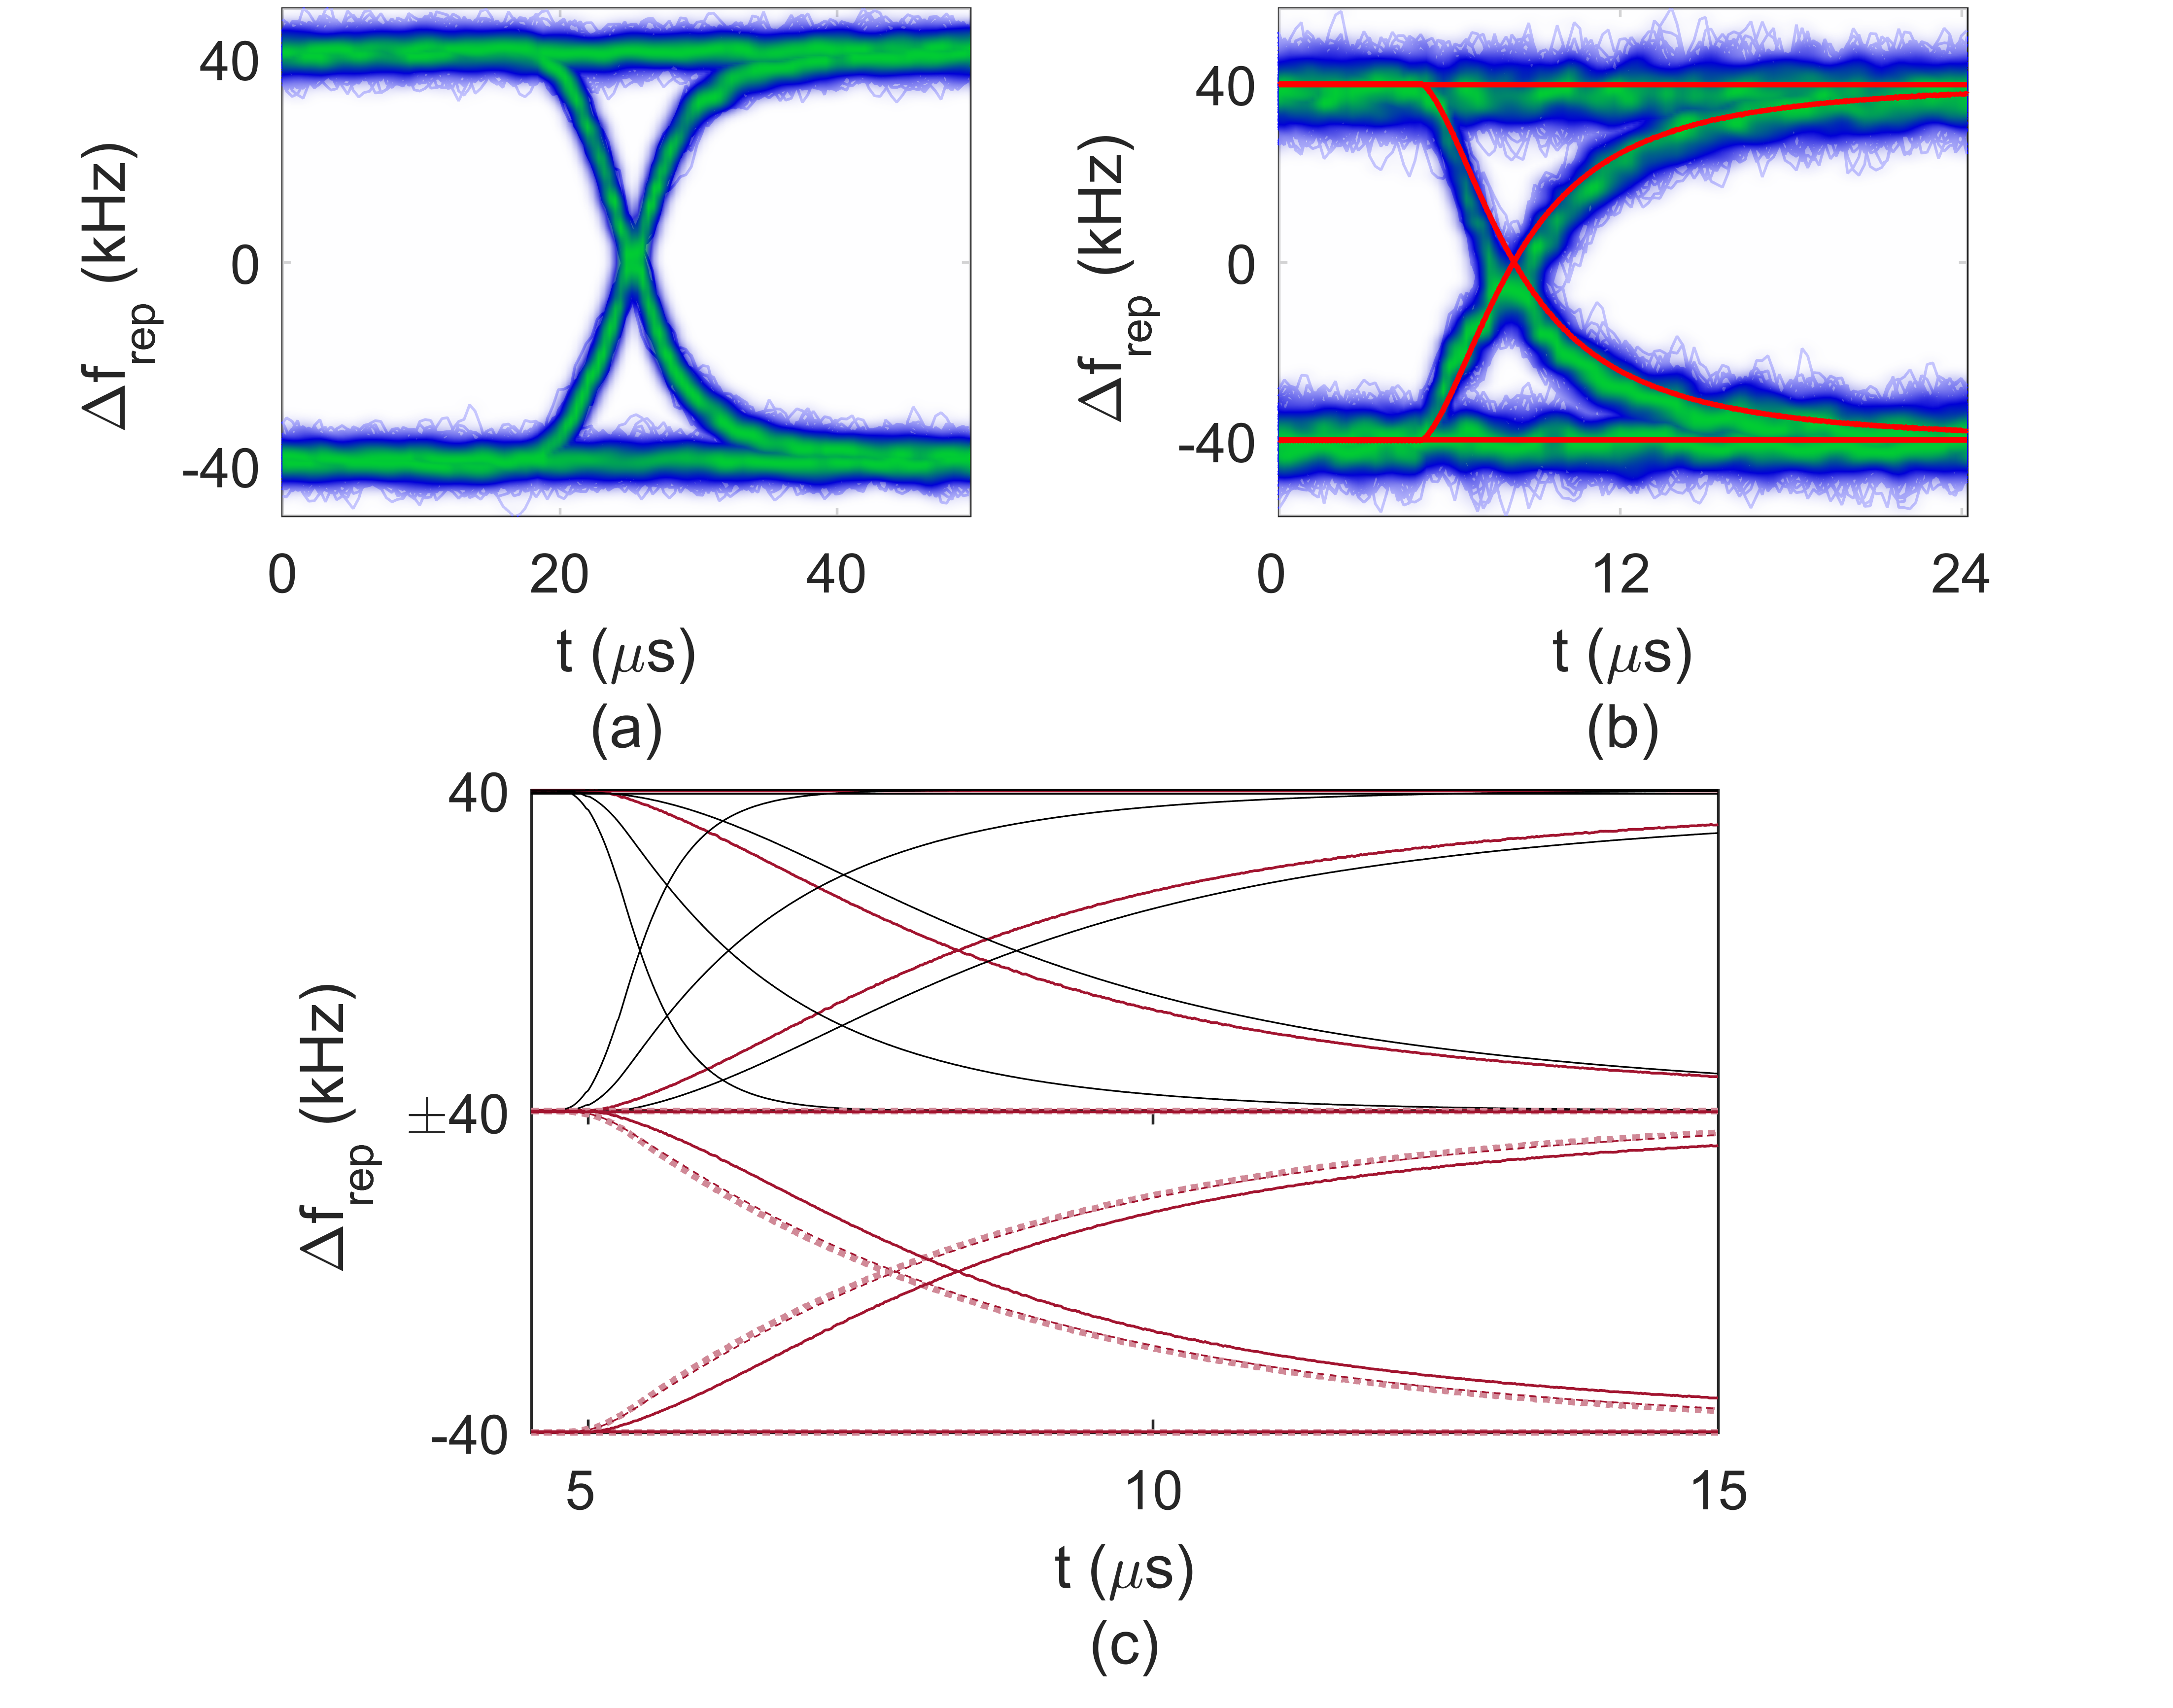
\includegraphics{\FigPath/Figures/PMPumping/PMeyediags.png}
	\end{center}
	\caption[Repetition-rate switching driven by a phase-modulated pump laser]{\textbf{Repetition-rate switching driven by a phase-modulated pump laser.} (a) Measured eye-diagram showing the switching capability of the soliton pulse train's repetition rate as $f_{PM}$ is switched over $\pm$40 kHz with 10 $\mu$s transition time. (b) The same with 60 ns transition time, with an LLE simulation of the dynamics (red) overlaid. The simulation parameters are $\delta_{PM}=0.9\pi$, $\Delta\nu=1.5$ MHz. (c) Simulated switching dynamics for various linewidths and modulation depths. Top: $\Delta\nu$=10 MHz (fastest, left), 3 MHz, and 1.4 MHz (traces shown in solid black). Bottom: depths of $2\pi$ and $6\pi$ (dashed red, curves nearly overlap). In each, the other parameter matches the simulation in (c), which is shown again in solid red. }
	\label{fig:PMeyediags}
\end{figure} 

\section{Subharmonic phase modulation for high repetition-rate systems}

One apparent barrier to the use of a phase-modulated pump laser for single-soliton generation and manipulation is the electronically-inaccessible FSRs of some typical microcomb resonators. However, it is possible to overcome this challenge by phase modulating at a subharmonic of the FSR.  Simulations indicate that PM can directly excite single solitons with small modulation depth, e.g. $\delta_{PM}=0.15\pi$. In this limit, only the first-order PM sidebands are relevant, and their amplitude and phase relative to the carrier control the dynamics. For a small desired modulation depth defined by the relationship between the first-order sidebands and the carrier, it is possible to modulate at a frequency $f_{PM}\sim f_{FSR}/N$ so that the $N$\textsuperscript{th}-order PM sidebands and the carrier address resonator modes with relative mode numbers -1, 0, and 1. The depth of modulation at the frequency $f_{PM}$ can be chosen to fix the amplitudes of the $N$\textsuperscript{th}-order PM sidebands relative to the carrier and target a desired effective modulation depth. It is worth noting that when N is odd, phase modulation is recovered when the sidebands of order $-N$, 0, and $N$ address resonator modes -1, 0, and 1. When $N$ is even the result is pure amplitude modulation, such that the driving term takes the form $F(1+A \cos{\theta})$. Simulations indicate that this AM profile also enables spontaneous single-soliton generation under some circumstances, but we note that this modulation profile cannot be obtained from a standard Mach-Zehnder modulator, which provides a drive like $F \cos(\eta+\delta \cos{\theta})$; AM in general may be less useful than PM because schemes of comparable complexity do not always provide robust trapping of solitons to the same point in the co-moving frame at which they are generated.

Fig. \ref{fig:PMsubharmonic} presents an example of this technique. We simulate spontaneous soliton generation with PM at $f_{PM}=f_{rep}/N=f_{rep}/21$. The effective modulation depth is $0.15\pi$, which requires real modulation depth at the frequency $f_{PM}$ with depth $\delta_{PM}\sim8.3\pi$.  Because the phase modulation spreads the optical power into the PM sidebands, use of this technique requires higher optical power for the same effective pumping strength; in this example the optical power must be increased by $\sim$15.6 dB. A smaller real modulation depth could have been chosen to recover effective depth of $\delta_{eff}=0.15\pi$, but our chosen depth of $\sim8.3\pi$ gives better efficiency due to the higher ratio of the power in modes $0$, $\pm$21 to the total power in the spectrum. While the required modulation depth and pump power are higher with subharmonic phase modulation, neither is impractical. This technique could be used for spontaneous single-soliton generation in high-repetition rate systems; the example above indicates that it could be immediately applied in a 630 GHz-FSR resonator with 30 GHz phase modulation. 



\begin{figure}[htpb]
	\begin{center}
		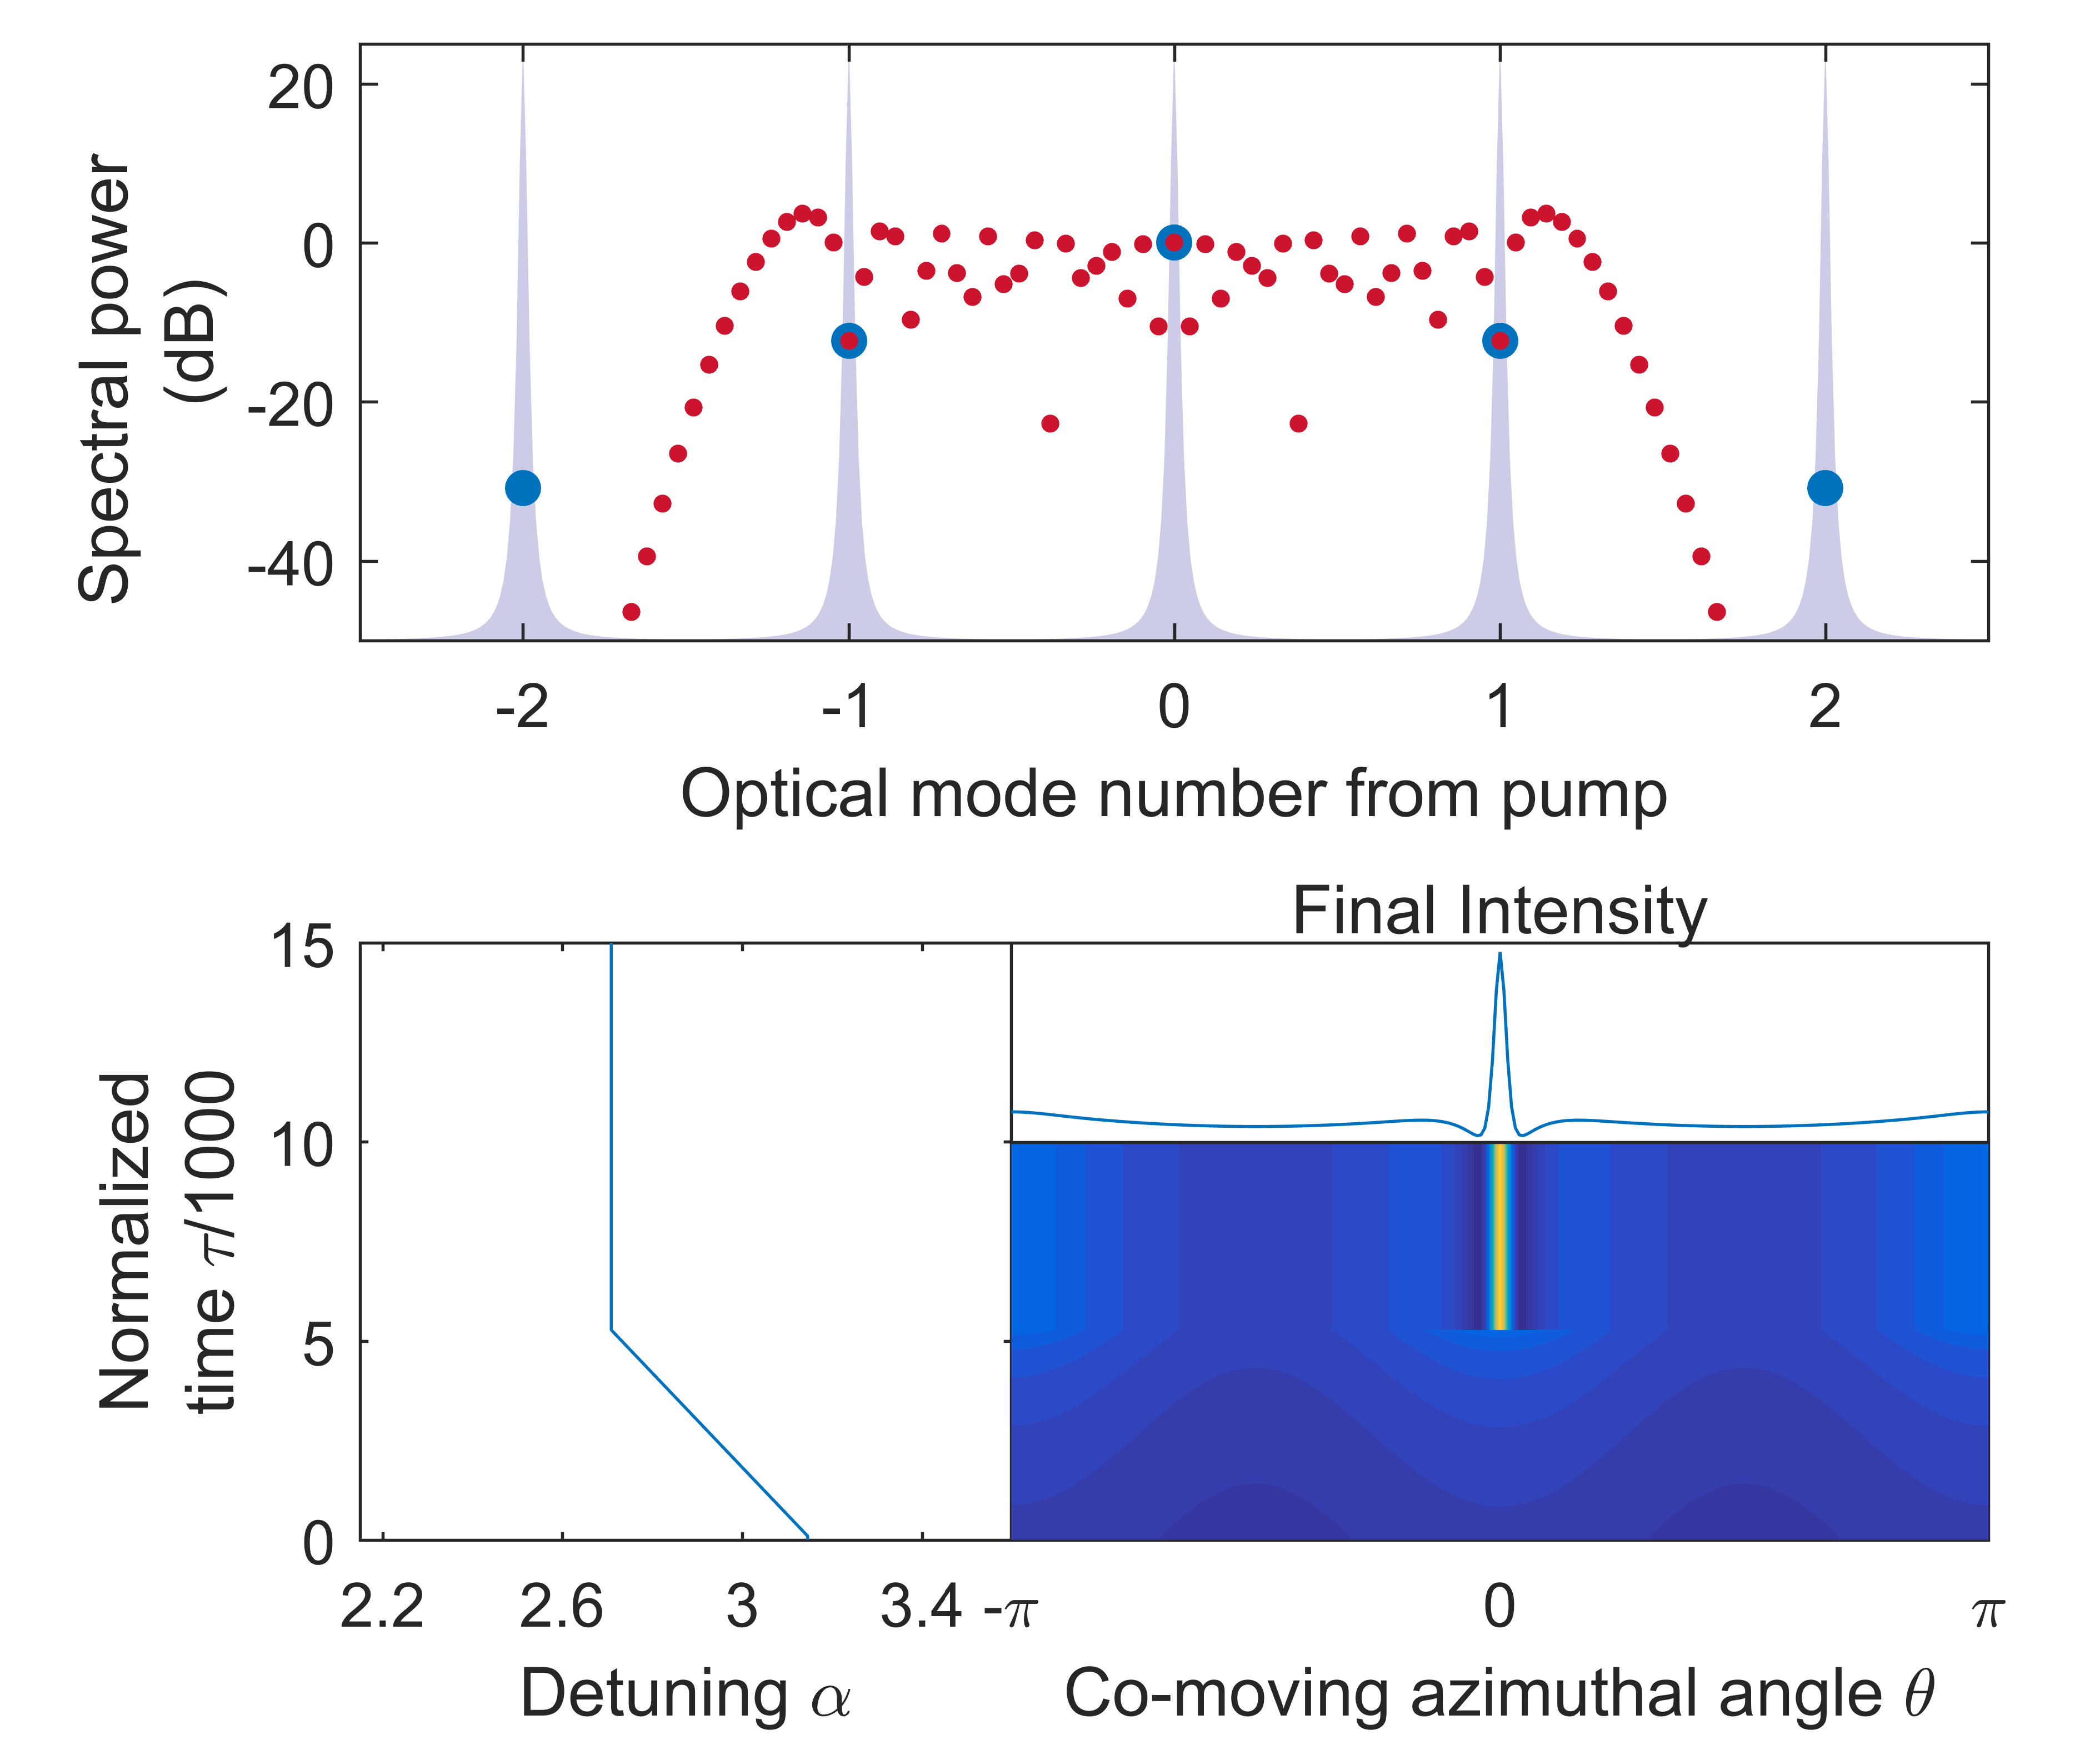
\includegraphics{\FigPath/Figures/PMPumping/PMsubharmonic.png}
	\end{center}
	\caption[Subharmonic phase modulation for high repetition-rate soliton generation]{\textbf{Subharmonic phase modulation for high-repetition-rate soliton generation.} (a) Spectra of PM at $f_{FSR}$ with depth $0.15\pi$ (blue) and at $f_{FSR}/21$ with depth $\sim$8.3$\pi$ (red). The relationships between the fields that address resonator mode numbers -1, 0, and 1 (as indicated by the gray Lorentzian curves) are the same in both cases. (b) LLE simulation of single-soliton generaiton using the subharmonic phase-modulation spectrum shown in red in panel (a). Only modes $n=0$, $\pm$21, $\pm$42,... of the phase-modulated driving field are coupled into the resonator and affect the LLE dynamics, with modes $|n|>$21 having negligible power. As $\alpha$ is increased from a large initial value, a soliton is spontaneously generated, exactly as in the case of phase modulation near the FSR.}
	\label{fig:PMsubharmonic}
\end{figure} 

%
%We demonstrate protected single-soliton formation and operation in a Kerr microresonator using a phase-modulated pump laser. Phase modulation gives rise to phase and amplitude variations in the resonator background, which in turn lead to an operation regime in which multi-soliton degeneracy is lifted and a single soliton is the only observable behavior. Direct excitation of single solitons is indicated by observed reversal of the characteristic ‘soliton step.’ Phase modulation also enables precise control of the soliton pulse train’s properties, and measured dynamics agree closely with simulations. We show that the technique can be extended to high repetition-frequency Kerr solitons through subharmonic phase modulation. These results facilitate straightforward generation and control of Kerr-soliton microcombs in integrated photonics systems. 
%
%
%
%Dissipative temporal cavity solitons in Kerr microresonators [1–3] have the potential to provide the revolutionary capabilities of frequency combs in a chip-integrable platform. This would extend the reach of frequency combs to applications in communications,  computation, and sensing with low size, weight, and power. Progress has come rapidly in the field of microresonator-soliton-based frequency combs, but for these combs to reach applications, simple, repeatable, and platform-independent methods of soliton generation and control are needed. The basic challenge is that solitons in microresonators are independent excitations, and a resonator can host zero, one, or many co-circulating solitons at a given pump-laser power and frequency, with each soliton giving rise to its own out-coupled pulse train. Further, under normal conditions solitons can only be generated by condensation from extended modulation-instability (MI) patterns (primary comb/Turing patterns, or noisy comb/spatiotemporal chaos) that provide appropriate initial conditions. Thermal stability must be maintained during the drop in intracavity power associated with the transition from a high duty-cycle MI pattern to a low duty-cycle soliton. A variety of schemes have been demonstrated to address these challenges and obtain single solitons [4–7], and many achieve excellent performance. In general these schemes increase experimental complexity, exploiting non-adiabatic variations in pump-laser power and frequency, and involve at least some amount of stochastic fluctuation in the output. 
%One notable possibility is modulation of the pump laser at a frequency near the resonator free-spectral range (FSR) [8–11], which can enable deterministic condensation of either one or zero solitons from an MI pattern. Further, it has been demonstrated that phase modulation (PM) can facilitate generation and control of single solitons [10,12,13]. Here we use PM at the FSR to deterministically excite single solitons directly from a chirped background that is stable elsewhere, as proposed in Ref.  [14]. Exiting the resonator is a train of solitons spaced by the round-trip time, as shown in Fig. 1a.  Importantly, no transient perturbation to the system parameters is required.
%Our results demonstrate a regime in which single-soliton operation is fundamentally protected, without the degeneracy between N=0,1, and many solitons that exists for a continuous-wave (CW) pump laser.  To motivate the experimental work that follows, we present theoretical results that illustrate the utility of a PM pump. We use the nonlinear partial-differential Lugiato-Lefever equation (LLE) with modification of the driving term for phase-modulation of depth δ_PM [1,14–17]:
%
%
%The normalized quantities used in the LLE are defined as follows [15]: ψ is the envelope for the intracavity field normalized so that |ψ|^2=1 at the absolute threshold for parametric oscillation; τ=t/2τ_γ, where t is the time and τ_γ=1/2πΔν is the cavity photon lifetime and Δν is the cavity resonance linewidth; α=2(ν_0-ν_pump )/Δν is the detuning between the pumped resonance with frequency ν_0 and the pump laser with frequency ν_pump; F is the pump strength normalized so that F^2=1 at the absolute threshold for parametric oscillation; and β_2=-2D_2/Δν<0 is the anomalous resonator dispersion, with D_2/2π=∂^2 ν_μ/∂μ^2 |_(μ=0)>0, where ν_μ represents the set of cavity resonance frequencies. The azimuthal angle θ co-rotates at the frequency f_PM, which is presently assumed to be equal to f_FSR.
%
%
%We perform simulations of the LLE to investigate soliton degeneracy for the range of pump-laser detunings overwhich solitons exist. These simulations use a fourth-order Runge-Kutta algorithm in the interaction picture [18] with adaptive step size [19]. A comparison of the resulting soliton energy-level diagrams for the CW case (δ_PM=0) and the PM case (δ_PM=π/2) are shown in Fig. 1b. We find that PM transforms the resonator excitation spectrum from a series of N=0,1,2,…,N_max solitons to a single level N=1 near threshold, eliminating degeneracy between these states. This occurs due to amplitude variations resulting from the phase modulation, with dispersion and nonlinearity providing PM-to-AM conversion. We can gain some insight into the origin of this effect by inserting the ansatz ψ(θ,τ)=ϕ(θ,τ)e^(iδ_PM  cos⁡θ ) into Eq. (1) [13].  By expanding the second-derivative term and setting derivatives of ϕ to zero we arrive at an equation for the quasi-CW background in the PM-pumped resonator:
%F=(γ(θ)+iα_eff (θ))ϕ-i|ϕ|^2 ϕ,	(2)
%where we have defined effective loss and detuning terms:
%γ(θ)=1+β_2/2 δ_PM  cos⁡θ,	(3)
%α_eff (θ)=α-β_2/2 δ_PM^2  sin^2⁡θ.	(4)
%
%
%
%
%
%This equation yields an approximate solution for ψ:
%ψ=(Fe^(iδ_PM  cos⁡θ ))/(γ(θ)+i(α_eff (θ)-ρ(θ)) ),	(5)
%where ρ(θ)=|ϕ(θ)|^2 is the (smallest real) solution to the cubic polynomial in ρ that results from calculating the modulus-square of Eq. (2). In neglecting the spatial derivatives of ϕ but retaining the derivatives of the phase term e^(iδ_PM  cos⁡θ ) we have made the approximation that the dominant effect of dispersion comes from its action on the existing broadband phase-modulation spectrum. This model reveals that amplitude variations in the quasi-CW background can be expected as a result of the spatially-varying effective loss and detuning terms that arise from the periodically-chirped pump laser.
%Fig. 1c compares the predictions of numerical LLE simulations (color) with the analytical model (black). The two agree quantitatively at small modulation depth (δ_PM=π/2, blue) and qualitatively at larger depth (δ_PM=4π, green). Both the simulations and the approximate analytic solution indicate that the background has two peaks per round trip in the presence of phase modulation, which suggests a mechanism for spontaneous single-soliton generation: At threshold the larger peak becomes locally unstable, and a soliton forms [20,21]. Moreover, it is known that if solitons exist elsewhere they are pushed to the larger peak by the background’s modulated phase [13]. This makes superpositions of N>1 solitons unstable and practically forbidden. Generation of single solitons then simply requires tuning the pump power and frequency to appropriate values, regardless of initial conditions. 
%The detuning for soliton generation can be estimated using Eq. (2) by calculating the value of α where ρ(θ=0)=1. This comes with a further approximation—simulations reveal that the critical detuning for soliton formation is near but not necessarily at ρ=1 because the spatial interval over which threshold is exceeded must have some minimum width. However, this approach quantitatively captures the behavior shown in Fig. 1b, predicting soliton generation at α=2.737.
%Because it is background intensity variations that result local MI and spontaneous soliton generation, it is natural to consider whether a similar technique can be employed using amplitude modulation (AM). In principle this can be done. However, to experimentally realize the robust single-soliton operation we describe below, the intensity modulation would need to yield a narrow cavity intensity maximum, and would therefore necessarily be broadband (e.g. pulsed pumping [11,21]), or would require supplementary PM to generate a trapping site for solitons. We are unaware of a straightforward implementation of AM for protected single-soliton operation that rivals the simplicity of the scheme presented here.
%We implement the approach described above to realize completely deterministic generation of single solitons without condensation from an extended pattern, summarized in Fig. 2. We use a 22 GHz-FSR silica ring resonator with Δν~1.5 MHz linewidth [22], pumped by a laser with normalized power F^2 between 2 and 6 that is phase-modulated at a rate f_PM~22 GHz with relatively small depth δ_PM~π. We overcome thermal instabilities [23] and control the detuning ν_0-ν_pump in real time using a frequency-agile pump [24], with an AOM-shifted probe for continuously monitoring the detuning. We decrease the detuning from a large initial value (~40 MHz), and a soliton is generated near 5 MHz (dependent upon the pump power and coupling condition). Measuring the power converted through FWM to new frequencies, the ‘comb power,’ reveals a step upon soliton formation, shown in Fig. 2a. This represents a reversal of the characteristic ‘soliton step’ that typically signals condensation of solitons from an extended pattern and indicates direct generation of a soliton from the background. After soliton generation, α may be increased again without loss of the soliton, consistent with Fig. 1b. We have verified that it is possible to turn off the PM while preserving the soliton (see also Ref.  [14]). 
%
%
%
%Automating soliton generation by repeatedly scanning the laser into resonance (detuning ~5 MHz) and back out again (20 MHz, far enough that the soliton is lost) has enabled reversible generation of 1000 solitons in 1000 trials over 100 seconds, with a 100 % measured success rate. Our probe-laser setup enables measurement of the detuning at which soliton generation occurs, which changes little from run to run. Fig. 2c presents a histogram of measurements for the generation of 160 solitons.
%Besides enabling protected sigle-soliton operation, PM pumping  also naturally provides timing and repetition-rate control, because the solitons are pushed towards the intracavity phase maximum [13]. This is illustrated in Fig. 3. In our experiments, the repetition rate of the out- coupled pulse train (f_rep) remains locked to f_PM over a bandwidth of ~±40 kHz. In Fig. 3a, we show a measured spectrogram of f_rep as f_PM  is swept sinusoidally over ±50 kHz. The repetition rate follows the PM except for glitches near the peaks of the sweep. In the inset of Fig. 3a we overlay the results of LLE simulations (see below) that qualitatively match the observed behavior. These simulations indicate that the periodic nature of the glitches is due to the residual pulling of the phase modulation on the soliton when the latter periodically cycles through the pump’s phase maximum. Our observed locking range of ~±40 kHz agrees well with an estimate δ_PM×D_2/2π~44 kHz [13] using the approximate measured value D_2=14 kHz per mode.
%Measured eye diagrams presented in Figs. 3b and 3c illustrate the switching of f_rep as f_PM is switched by 80 kHz around the soliton’s natural repetition rate. In Fig. 3b, f_PM is switched with 200 μs period and 10 μs transition time; in Fig. 3c it is switched with 100 μs period and 60 ns transition time. This data is obtained by detecting f_rep and passing the signal through two paths, one with an element that induces a frequency-dependent phase shift. From the resulting phase difference the repetition rate can be measured in real time. These eye diagrams show that the PM enables exquisite control of the soliton pulse train.
%We further explore the dynamics of repetition-rate switching by performing additional LLE simulations. We introduce the term +β_1  ∂ψ/∂θ to the right-hand side of Eq. (1), where β_1=-2(FSR-f_PM)/Δν represents a difference between the modulation frequency and the FSR 
%
%
%
%of the resonator near the pump wavelength [13,14];  β_1 may be varied in time.  In Fig. 3c we overlay a simulation of switching conducted for parameters (Δν=1.5 MHz, δ_PM=0.9 π) near the experimental values, and the agreement between measurements and simulation indicates that the measurements are consistent with fundamental LLE dynamics. We present the results of additional simulations in Fig. 3d; the basic observation is that the switching speed of f_rep is limited by the resonator linewidth, and can be modestly improved by increasing δ_PM.
%One apparent barrier to the use of a phase-modulated pump laser for protected single-soliton generation and manipulation is the electronically-inaccessible FSRs of some typical microcomb resonators. However, it is possible to overcome this challenge by phase modulating at a subharmonic of the FSR.  Simulations indicate that PM can directly excite single solitons with small modulation depth, e.g. δ_PM=0.15π. In this limit, only the first-order PM sidebands are relevant, and their amplitude and phase relative to the carrier control the dynamics. For a small desired modulation depth defined by the relationship between the first-order sidebands and the carrier, it is possible to modulate
%
%
%at a frequency ~f_FSR/N so that the N^th-order PM sidebands and the carrier address resonator modes with relative mode numbers -1, 0, and 1. The depth of modulation at the frequency f_FSR/N can be chosen to fix the amplitudes of the N^th-order PM sidebands relative to the carrier and target a desired effective modulation depth. It is worth noting that when N is odd, phase modulation is recovered when the sidebands of order -N,0, and N address resonator modes -1, 0, and 1. When N is even the result is pure amplitude modulation, such that the driving term takes the form F(1+A cos⁡θ). Under some circumstances this AM profile also enables spontaneous single-soliton generation, but we note that this modulation profile cannot be obtained from a standard Mach-Zehnder modulator, which provides a drive like F cos⁡(η+δ cos⁡θ ).
%Fig. 4 presents an example of this technique. We simulate protected single-soliton generation with PM at f_mod=f_rep/N=f_rep/21. The effective modulation depth is 0.15π, which requires real modulation depth at the frequency f_mod with depth δ_PM~8.3π.  Because the phase modulation spreads the optical power into the PM sidebands, use of this technique requires higher optical power for the same effective pumping strength; in this example the optical power must be increased by ~15.6 dB. While the required modulation depth and pump power are higher with subharmonic phase modulation, neither is impractical. This technique could be used for protected single-soliton generation in high-repetition rate systems; the example above indicates that it could be immediately applied to deterministic single-soliton generation in a 630 GHz-FSR resonator with 30 GHz phase modulation. 
%In this work, we have shown that PM-pumping fundamentally changes a resonator’s excitation spectrum and enables a new regime of protected single-soliton operation. The technique is applicable to resonators with electronically accessible f_rep, which are important components of proposals for photonic integration of Kerr-solitons  [25,26], and can reach higher repetition-rate systems via subharmonic modulation. After soliton generation, the PM can optionally be turned off, recovering the properties of the non-PM soliton. We expect this technique to enable new experiments. For example, PM-pumped solitons are generated with known absolute timing, enabling immediate transduction of the modulation phase onto
%
%
%
%
%the pulse train; this is impossible with solitons stochastically condensed from an extended pattern. Our work brings microresonator solitons closer to applications.
  %read 6-27
% \chapter{Soliton crystals in microresonators} \label{chap:SolitonCrystals}

This chapter presents results on the self-organization of ensembles of solitons in optical microring resonators. These results involve physics beyond the basic LLE model for Kerr-comb formation, as is described in Sec. \ref{sec:crystallizationmechanism}. These experiments are performed using laser-machined silica microrod resonators \cite{DelHaye2013} and chemically-etched microdisk \cite{Lee2012} resonators with $\sim$25 GHz and $\sim$16.5 GHz FSR, respectivel; however, but the physical mechanism for the self-orgainzation that we describe applies to any resonator that supports multiple transverse modes. We refer to these self-organized soliton ensembles as `soliton crystals,' which extends an analogy to condensed-matter physics that has been made in other nonlinear-optical systems, including single-pass nonlinear fiber systems \cite{Zajnulina2017} and harmonically mode-locked fiber lasers \cite{Haboucha2008,Amrani2011a}, where a different mechanism for soliton crystallization that is based on two distinct timescales of the laser medium was identified \cite{Haboucha2008c}. It is interesting to note that the spatiotemporal chaos exhibited by Kerr combs was referred to as a `soliton gas' in early studies of nonlinear dynamics in passive fiber-loop resonators \cite{Malomed1998,Mitschke1998,Schwache1997}. 

\section{Spectral and temporal characteristics of soliton crystals}

Soliton crystals in Kerr resonators are soliton ensembles in which each soliton lies on a lattice site $\theta_n= 2\pi n/N$ in the azimuthal co-moving frame, where $N$ is a lattice parameter that arises from the fundamental physics of the system as described below and $n$ indexes over the lattice sites. In the soliton crystals presented below there are many more available lattice sites than solitons, so that a fraction of the lattice sites are occupied. In the frequency domain, the temporal ordering of pulses in a soliton crystal corresponds to a highly modulated optical spectrum that exhibits distinctive features. 

We present plots illustrating the spectral and temporal characteristics of an example soliton crystal in Fig. \ref{fig:SCjiggled}. Fig. \ref{fig:SCjiggled}a shows an experimental measurement of a soliton crystal spectrum. This spectrum exhibits prominent comb modes similar to primary-comb lines, and underlying these primary-comb lines are single-FSR-spaced spectral lobes. We can understand this spectrum through the basic superposition principle of the electric field: The primary comb spectrum with spacing $N\times f_{FSR}$ corresponds to a train of $N$ uniformly spaced pulses in the resonator; here $N=24$. To this pulse train we add an \textit{out-of-phase} pulse $S_-$ that coincides in time with one of the existing pulses---in the time domain this corresponds to the introduction of a vacancy into the pulse train, while in the frequency domain this corresponds to the addition (in the phase-sensitive field quantity) of the primary-comb spectrum and the spectrum of the single, out-of-phase soliton. We then add a second soliton $S_+$  to the pulse train, this one \textit{in phase} with the existing pulses and slightly temporally shifted from the vacancy. The time-domain result is a pulse train with one pulse displaced from its expected position based on uniform spacing. In the frequency domain, the positions of the pulses $S_+$ and $S_-$ correspond to different linear spectral phase shifts on each of their individual spectra; when these spectra are added together the result is spectral interference that is periodic in frequency. This gives rise to the lobes beneath the primary-comb lines; the frequency period of the interference is inversely proportional to the separation between the pulses $S_+$ and $S_-$ in time.

We illustrate this principle by plotting pulse trains exhibiting a shifted pulse in Fig. \ref{fig:SCjiggled}b, and show their calculated spectra in Fig. \ref{fig:SCjiggled}a. These pulse trains are constructed using the analytical approximation to soliton ensembles provided by Eq. \ref{eq:LLEsolens}. The pulse train shown in orange is composed of solitons pinned to sites on a lattice, and the pulse train shown in blue is obtained from this first pulse train by introducing a small random displacement to the position of each pulse. The effect of this small position jitter is apparent in the calculated spectra in Fig. \ref{fig:SCjiggled}a---the highly-distinctive spectral characteristics of the soliton crystal are eroded. In fact, it is a general property of the soliton-crystal spectra that we present in this chapter that the contrast and definition of the distinctive spectral characteristics depends on the high precision with which the pulses fall on the lattice sites.

%The observed crystal spectrum corresponds to such a pulse train with a single vacancy, where a pulse is missing. The effect of this vacancy on the spectrum can be understood by considering the addition of an \textit{out-of-phase} pulse $S_-$ to a primary-comb pulse train, where $S_-$ coincides in time with one of the existing pulses---in the time domain this corresponds to removal of one of the pulses, while in the spectral domain this corresponds to the addition (in the phase-sensitive field quantity) of the primary-comb spectrum and the spectrum of the single, out-of-phase soliton. The soliton crystal spectrum shown in Fig. \ref{fig:SCjiggled} can also be understood this way: If a second soliton $S_+$ is added to the initial primary-comb pulse train, this one \textit{in phase} with the existing pulses and slightly temporally shifted from the vacancy, the result is a pulse train with one pulse displaced from its expected position based on uniform spacing. In the frequency domain, the positions of the pulses $S_+$ and $S_-$ correspond to different linear spectral phase shifts on each of their individual spectra; when these spectra are added together (in the phase-sensitive field quantity) the result is spectral interference that is periodic in frequency. This gives rise to the lobes beneath the primary-comb lines; the period (in frequency) of the interference is inversely proportional to the separation between the pulses $S_+$ and $S_-$ in time.


%
%
%An example soliton-crystal spectrum and time-domain waveform are presented in Fig. \ref{fig:SCjiggled}, where we demonstrate that the characteristic nature of the crystal spectrum is destroyed by small random displacement of the solitons from their lattice sites. We have observed a wide variety of crystal configurations, and we present some of them in Sec. \ref{sec:SCtaxonomy}; to characterize this highly-degenerate configuration space we adopt terminology from condensed matter physics to describe soliton crystal structure and defects. 

\begin{figure}[htpb]
	\begin{center}
		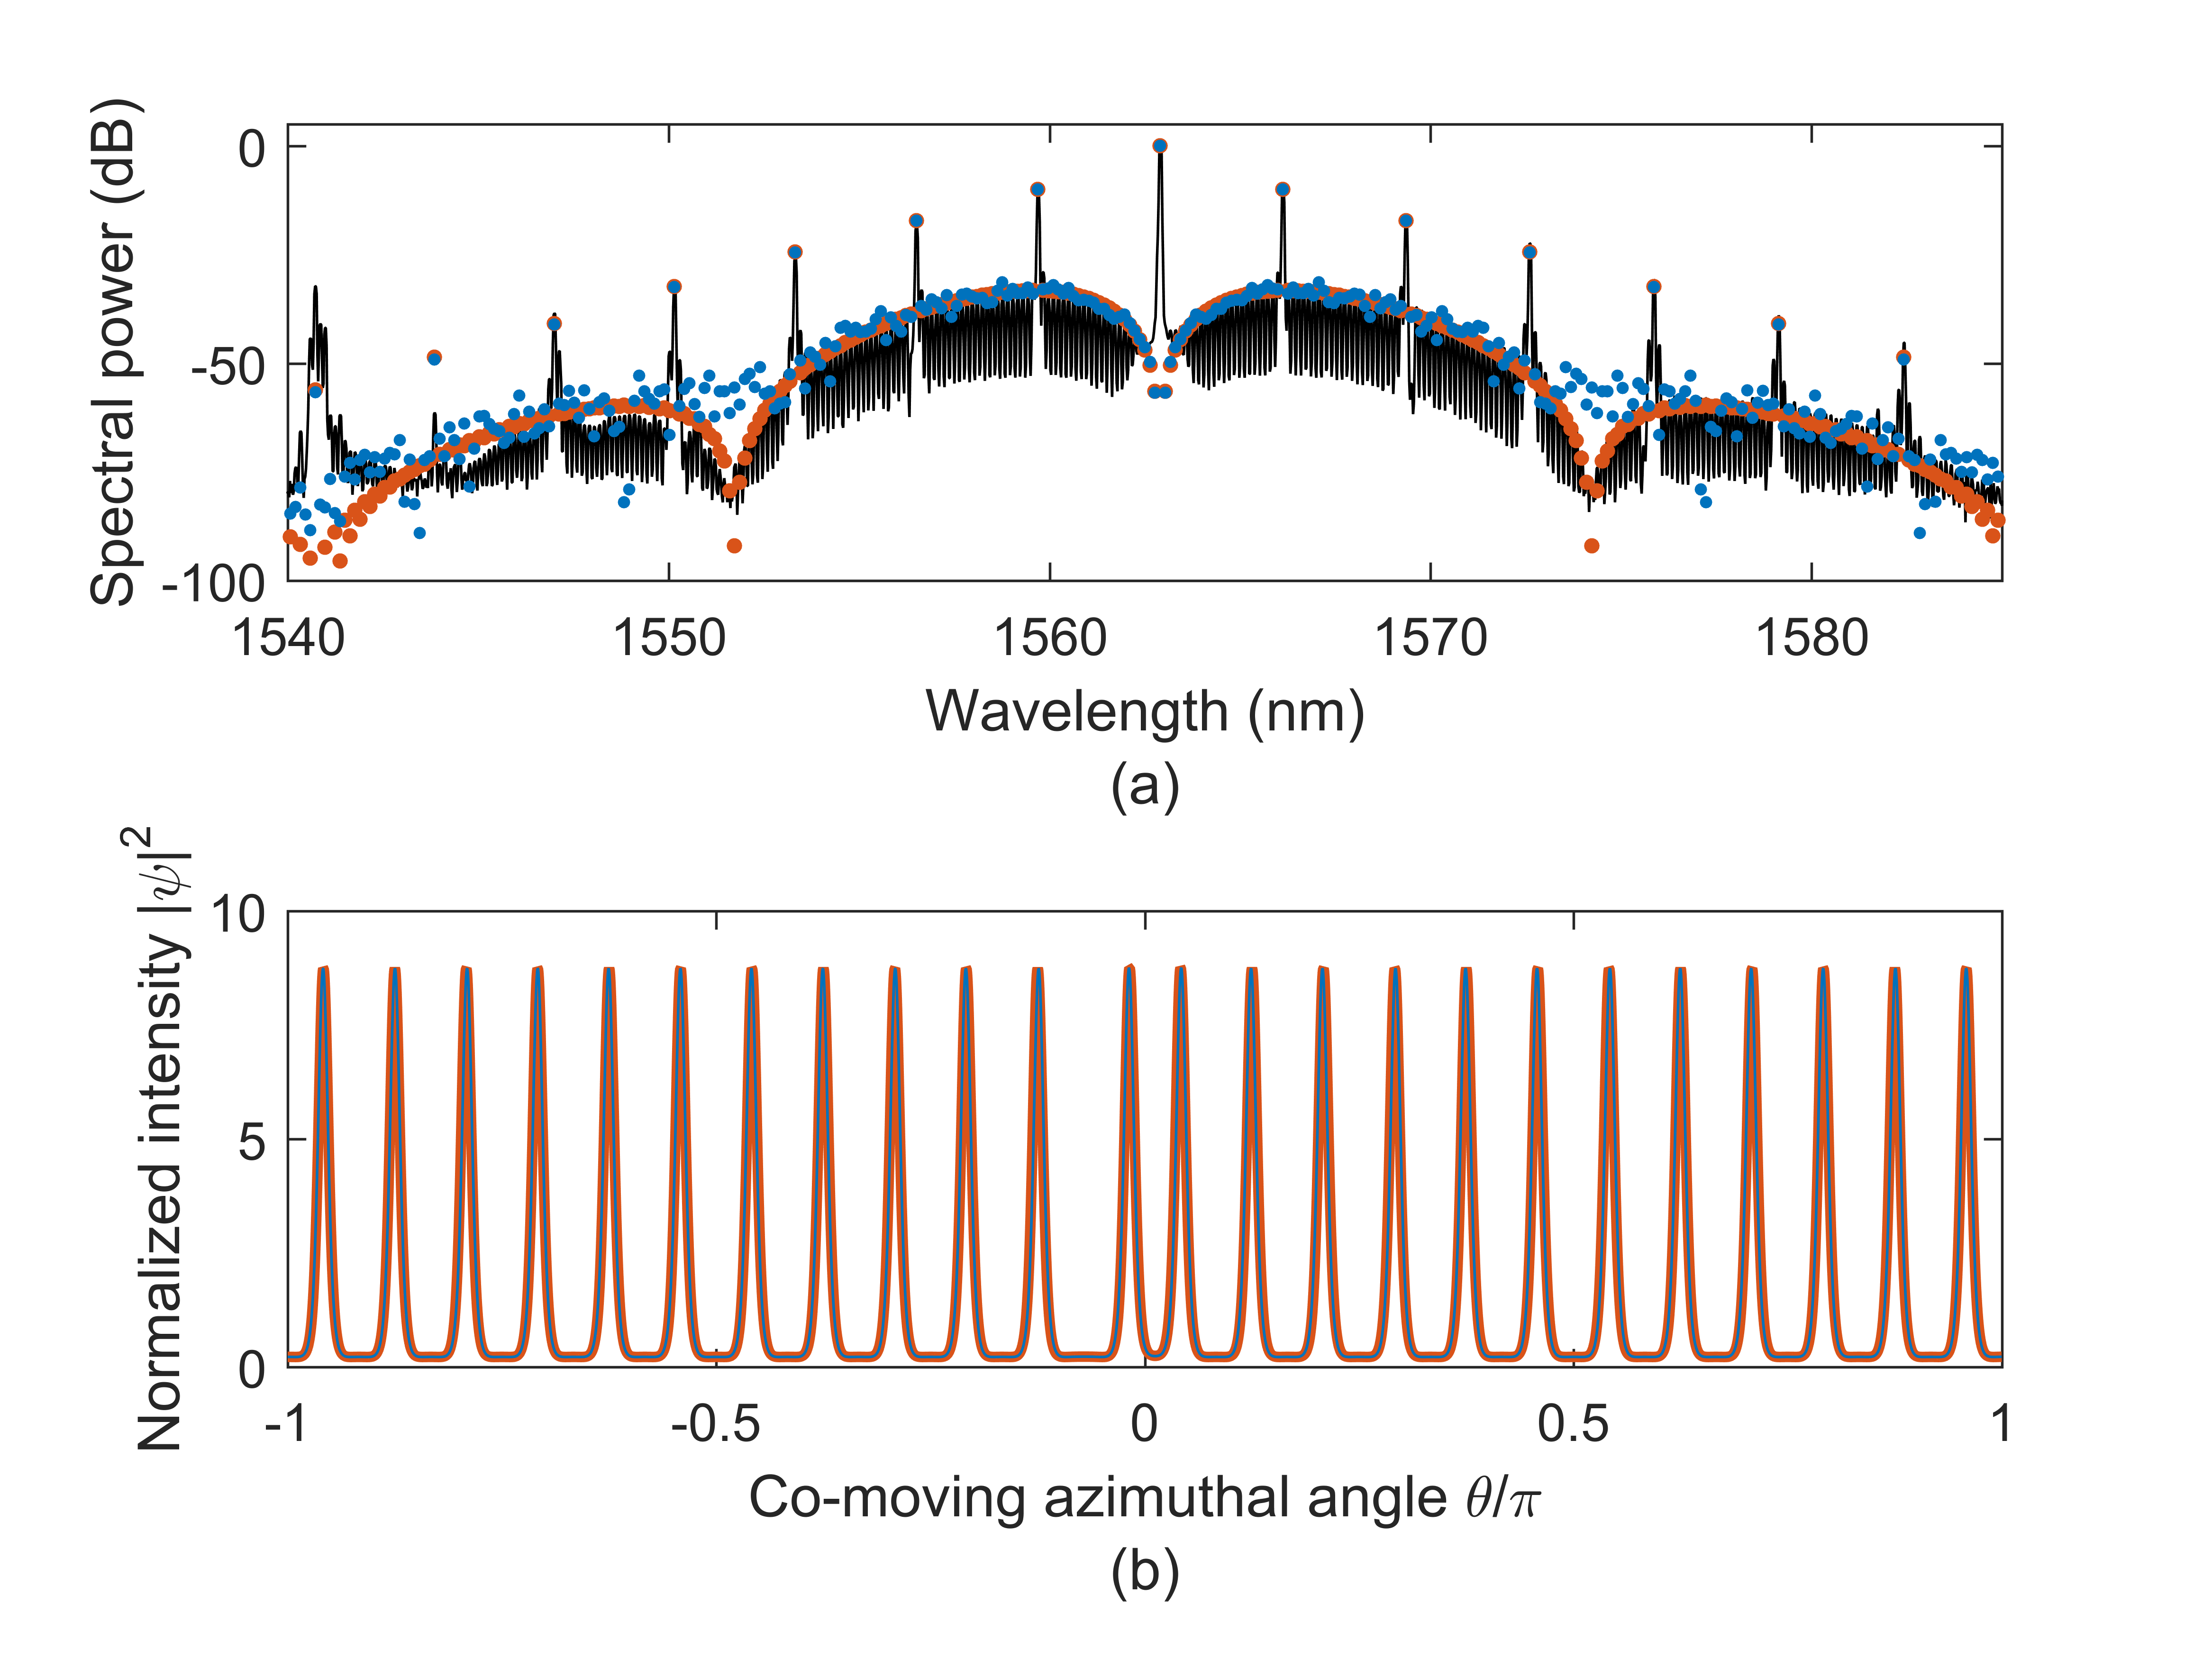
\includegraphics{\FigPath/Figures/SolitonCrystals/SCjiggled_v2.png}
	\end{center}
	\caption[Spectral contrast of a soliton crystal]{\textbf{Spectral contrast of a soliton crystal.} (a) Experimental measurement of a soliton-crystal spectrum (black), along with two approximations to the crystal's time-domain waveform as a soliton ensemble, according to Eq. \ref{eq:LLEsolens}. Shown in orange is the spectrum of an ensemble of solitons pinned to sites on a lattice with spacing $2\pi/(7\times24)$; here the majority of the pulses are separated from their neighbors by seven lattice sites, but one pulse is displaced by two lattice sites from its expected position. Shown in blue is a calculation of the spectrum that results when random (uniformly distributed) jitter is imposed on the same pulse positions; the range of the jitter is $\pm$ 3 $\%$ of the typical inter-soliton spacing $2\pi/24$. (b) Time-domain traces corresponding to the spectra shown in (a). There is no readily apparent difference between the positions of the pulses in two pulse trains because the magnitude of the imposed jitter is small; nevertheless the definition of the distinctive spectral features is eroded by the jitter.}
	\label{fig:SCjiggled}
\end{figure} 

\section{Soliton crystal generation}

Soliton crystals are characterized by stable, dense occupation of the resonator by soliton pulses, and this dense occupation comes with high circulating power relative to single solitons or few-soliton ensembles. This important fact allows soliton crystals to be generated with decreasing pump-laser frequency scans across the resonance that are adiabatic---slow enough that both the resonator temperature and the state of the comb $\psi$ are maintained at values\footnote{This terminology is a bit imprecise when applied to chaotic Kerr-combs that evolve with time; in this case the chaos exhibits the same behavior at each point in the scan that would be expected if $\alpha$ and $F^2$ were held fixed.} that correspond to the instantaneous $\alpha$ and $F^2$ parameters throughout the scan. We demonstrate generation of a soliton crystal in a slow scan in Fig. \ref{fig:SCexample}; it is interesting to contrast the continuity of the taper-transmission trace with the staircase-like nature of the same measurement exhibited in the generation of a few-soliton ensemble (see e.g. Ref. \cite{Herr2014} and the discussion in Chap. \ref{chap:microresonators}). Slower scans than the one presented in Fig. \ref{fig:SCexample} are possible, and in fact we have generated soliton crystals by tuning the pump-laser frequency arbitrarily slowly by hand.

\begin{figure}[htpb]
	\begin{center}
		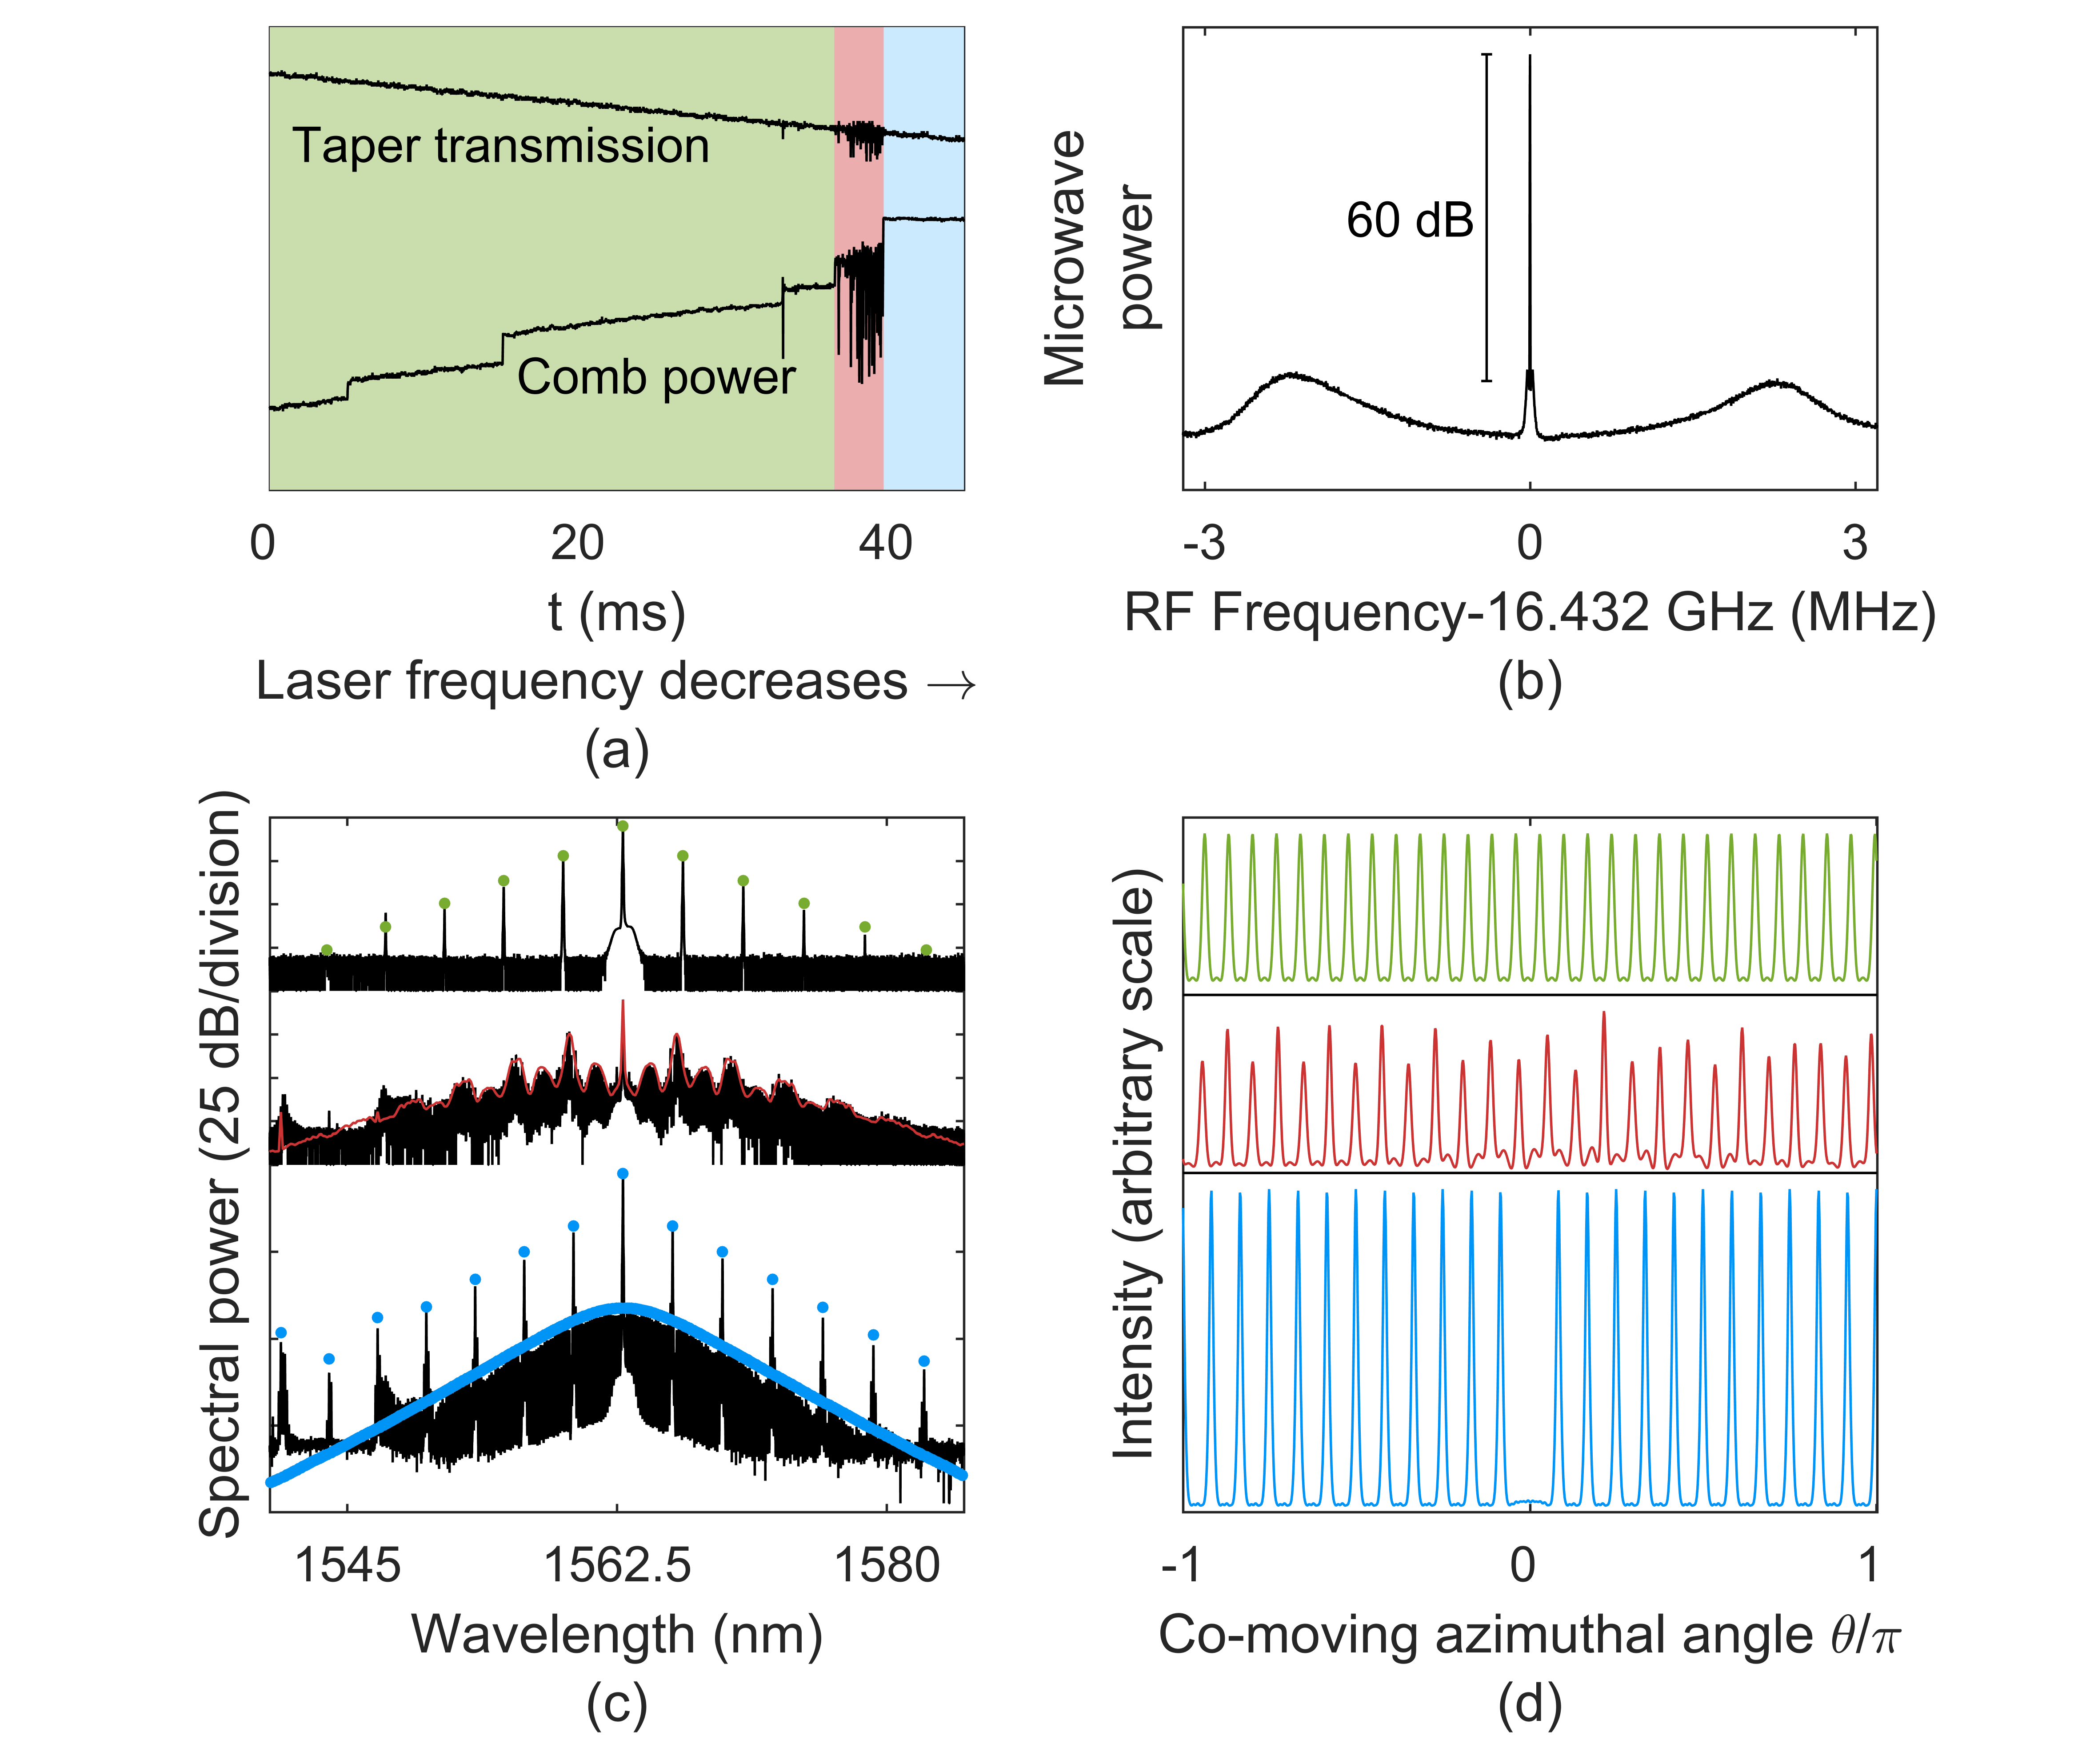
\includegraphics{\FigPath/Figures/SolitonCrystals/SCexample.png}
	\end{center}
	\caption[Generation and characterization of a soliton crystal]{\textbf{Generation and characterization of a soliton crystal.} (a) Measurements of the power transmitted past the resonator (`Taper transmission') and this power with the pump frequency filtered out (`Comb power') during crystal generation with a scan that proceeds through primary-comb (green), chaotic (red), and soliton crystal (blue) regimes. The resonator's thermal response leads to the non-Lorentzian taper transmission profile, and the continuity of the taper transmission trace upon soliton crystal condensation indicates that the intracavity power of the soliton crystal is matched to the chaos that precedes it. (b) Narrow measured RF beat for the repetition rate of the soliton crystal is indicative of a coherent comb, in contrast with the chaotic state. (c) Progression of the optical spectrum through the scan, with experimental data (black) obtained by halting the scan at the appropriate point, and LLE simulations (with a perturbation as described in Sec. \ref{sec:crystallizationmechanism}) in color. The simulated spectrum for the chaotic state shown in red is a time average. (d) Simulated time-domain traces corresponding to the simulated spectra in (c). The simulated intensity for the chaotic state is a snapshot. The soliton crystal shown in blue is a uniform pulse train with a single vacancy (see text).}
	\label{fig:SCexample}
\end{figure} 

\section{Mechanism of soliton crystallization} \label{sec:crystallizationmechanism}

%Figs. \ref{fig:SCexample}c and d present the optical spectrum and simulated corresponding time-domain waveform of a soliton crystal. This spectrum consists of widely-spaced primary-comb lines that are separated by many resonator FSR superposed with an underlying $\mathrm{sech}^2$ spectrum of the kind that corresponds to a single soliton. In fact, this spectrum can be understood through the basic superposition principle of the electric field: The primary comb spectrum with spacing $N\times f_{FSR}$ corresponds to a train of $N$ uniformly spaced pulses in the resonator. The observed crystal spectrum corresponds to such a pulse train with a single vacancy, where a pulse is missing. The effect of this vacancy on the spectrum can be understood by considering the addition of an \textit{out-of-phase} pulse $S_-$ to a primary-comb pulse train, where $S_-$ coincides in time with one of the existing pulses---in the time domain this corresponds to removal of one of the pulses, while in the spectral domain this corresponds to the addition (in the phase-sensitive field quantity) of the primary-comb spectrum and the spectrum of the single, out-of-phase soliton. The soliton crystal spectrum shown in Fig. \ref{fig:SCjiggled} can also be understood this way: If a second soliton $S_+$ is added to the initial primary-comb pulse train, this one \textit{in phase} with the existing pulses and slightly temporally shifted from the vacancy, the result is a pulse train with one pulse displaced from its expected position based on uniform spacing. In the frequency domain, the positions of the pulses $S_+$ and $S_-$ correspond to different linear spectral phase shifts on each of their individual spectra; when these spectra are added together (in the phase-sensitive field quantity) the result is spectral interference that is periodic in frequency. This gives rise to the lobes beneath the primary-comb lines; the period (in frequency) of the interference is inversely proportional to the separation between the pulses $S_+$ and $S_-$ in time.

The time-domain waveforms we have considered so far are not stable in evolution under the LLE. For each, the observed width of the spectrum fixes the ratio between $\alpha$ and $\beta$, as seen from Eq. \ref{eq:LLEsoliton}. This ratio then fixes the temporal duration of the solitons, in turn determining the characteristic length of their interactions. When an attempt to simulate the crystal according to the LLE is made with parameters that give agreement with the measured width of the optical spectrum (e.g. $F^2$=3.7, $\alpha=3.77$, and $\beta=-0.0054$ for the crystal in Fig. \ref{fig:SCexample}c and d), it is found that pair-wise attractive interactions between solitons lead to collapse of the crystal, as shown below in Fig. \ref{fig:SCexamplesim}.

A stabilization mechanism that goes beyond the physics of the LLE is responsible for the stability of soliton crystals. The stabilization mechanism for the crystals we present here arises from avoided mode crossings in the resonator spectrum. As discussed in Sec. \ref{sec:OMRR}, the resonators used in these experiments support multiple families of circulating modes, each with its own transverse spatial intensity profile and free spectral range. Although the modes in different families are in principle orthogonal, coupling between them can be provided by perturbations, for example by the coupling waveguide or tapered fiber used to drive the resonator, or anomalies in the resonator fabrication that break the resonator symmetry. When a coupling exists between modes that are sufficiently close in frequency, the modes become hybridized and their frequencies become displaced \cite{Haus1991}. The effect of this coupling and the associated perturbation to the resonator mode spectrum on Kerr-comb generation has been investigated \cite{Savchenkov2012}, and it has been found that avoided mode crossings can inhibit soliton generation in anomalous-dispersion resonators \cite{Herr2014a,Yi2015}, while they can facilitate the formation of Kerr-combs in normal-dispersion resonators \cite{Liu2014a,Xue2015,Bao2017}. 


%A `mode family' corresponds to a set of circulating modes that have different azimuthal mode numbers but (approximately, neglecting wavelength-dependent effects) the same transverse spatial mode profile. As discussed in Sec. \ref{sec:ec;OMRR}, some resonators support multiple mode families, each with its own free spectral range at a given wavelength. If a coupling exists between two modes that are sufficiently close in frequency, the frequencies of the modes become displaced from their frequencies in the absence of this coupling \cite{Haus1991}. This affects Kerr-comb generation in the affected mode families, because the local detuning between the resonator modes and the Kerr-comb modes is changed as a result of the mode crossing. This comb-resonator detuning change may either enhance or inhibit nonlinear frequency conversion to the effected Kerr-comb modes, thereby changing the amplitude of these modes in the comb spectrum. 

Here we are interested specifically in the impact of an avoided mode crossing on the temporal waveform of a soliton. For simplicity, we make the approximation that a single mode of the Kerr comb with number $\mu_\times$ is affected by the mode crossing. This approximation neglects the fact that avoided mode crossings between two families typically span a range of modes as the mode frequencies traverse each other in frequency space due to a small fractional difference between the free-spectral ranges of the two mode families; this can be observed in many of the experimental spectra presented in this chapter. However, we find that the single-mode assumption is generally sufficient for modeling the stability of the soliton crystals that we observe.

The perturbation of the frequency of a resonator mode $\mu_\times$ that is far from the pumped mode $\mu=0$ affects the local detuning of the comb from the resonator. When this local comb-resonator detuning is decreased, the efficiency of nonlinear frequency conversion to mode $\mu_\times$ can be increased. This increases the amplitude of mode $\mu_\times$ in the soliton's spectrum, and the resulting change to the time-domain waveform can be understood by considering this increase as the addition of extra CW light at the frequency of mode $\mu_\times$. This extra CW light leads to the introduction of periodic intensity oscillations in the background on which the soliton rides as it beats against the existing background at the pump frequency. The new background wave in the cavity has a period of $2\pi/\mu_\times$ in the angular coordinate $\theta$. 

When several of these perturbed solitons co-propagate in a resonator, they interact through their extended waves and arrange themselves such that the waves constructively interfere \cite{Wang2017}. Each soliton then lies at the peak of a single extended background wave in the resonator, similar to predictions for bichromatically pumped Kerr combs \cite{Hansson2014}. Importantly, temporal separations between solitons are therefore required to be multiples of this wave's period, and the wave stabilizes the crystal against the attractive interactions discussed above. Furthermore, the wave's amplitude, and thus the strength of the crystal against perturbations, increases with the number of co-propagating perturbed solitons. Within the assumption of single-mode perturbation of the comb's spectrum, this interaction has infinite range. 

We note that the mechanism observed here builds on previous reports of related phenomena. It has been shown that local interactions between cavity solitons can arise through decaying oscillatory tails \cite{Skryabin1999}, leading to the formation of small, locally ordered soliton molecules; this effect appears to be significant in Kerr ring resonators only at small detunings \cite{Parra-Rivas2017}. Additionally, it has been shown that the injection of a second CW laser into a passive fiber-ring resonator can result in the generation of uniform distributions of solitons \cite{Wabnitz1996}. The mechanism we report here can be viewed as a variant of this CW-soliton interaction in which the `injected' CW laser is provided by the solitons themselves through the affect of the mode crossing on the solitons' spectra.

We connect this discussion to the soliton-crystal spectrum presented in the bottom trace of Fig. \ref{fig:SCexample}c---this spectrum exhibits excess power near pump-referenced modes numbers $\mu_{\times,1}=5\times24=120$ (1547 nm) and $\mu_{\times,2}=7\times24=168$  (1541 nm), where 24 FSR is the spacing of the prominent primary-comb lines. Also visible is suppressed comb generation where the comb-resonator detuning has been increased. 

\subsection{Simulation of soliton crystals}

To incorporate the stabilization mechanism described above into numerical simulations, we insert into the LLE a reduced comb-resonator detuning on a single mode $\mu_\times$. The mode-dependent comb-resonator detuning can be calculated as:
\begin{align}
\alpha_\mu&=-2(\omega_p+\omega_\mu-D_1)/\Delta\omega_{tot},\\
&=\alpha-\beta\mu^2/2.
\end{align}

Here $\omega_p$ is the frequency of the pump laser, $\omega_\mu$ is the set of cavity resonance frequencies referenced to the pumped mode, and $D_1=\partial\omega_\mu/\partial\mu|_{\mu=0}$ is the resonator's FSR at the pumped mode and is also assumed to be the comb's repetition rate. The dispersion operator is applied in the frequency domain in numerical simulations of the LLE (see \ref{app:numericalsims}), which facilitates inclusion of $\delta$-function perturbations to the comb-resonator detuning as:
\begin{equation}
\alpha_\mu=\alpha-\beta\mu^2/2+\Delta\alpha_\mu,
\end{equation}
where
\begin{equation}
\Delta\alpha_\mu=2(\omega_\mu-\omega_{\mu,0})/\Delta\omega_{tot}
\end{equation}
is the normalized change in the frequency of mode $\mu$ from the expected frequency $\omega_{\mu,0}$. 

We demonstrate the stabilization mechanism and the simulation method by presenting a simulation of the crystal in Fig. \ref{fig:SCexample}c. The simulation is shown in Fig. \ref{fig:SCexamplesim}. This figure illustrates both the rapid timescale over which the stabilization mechanism acts and the instability of the crystal in the absence of the stabilization mechanism. To explain the stability of this 23-soliton crystal and the apparently exact circumferential spacing of the pulses by $2\pi/24$ radians, it is sufficient to incorporate into the LLE a reduced comb-resonator detuning on only mode 120 or on mode 168, where the excess power is largest. The crystal is then a steady-state solution of the resulting perturbed LLE.

%We note that a phenomenological application of coupled-mode theory \cite{Haus1991} could be used to calculate the full perturbation to the soliton spectrum by the mode crossing, 

\begin{figure}[htpb]
	\begin{center}
		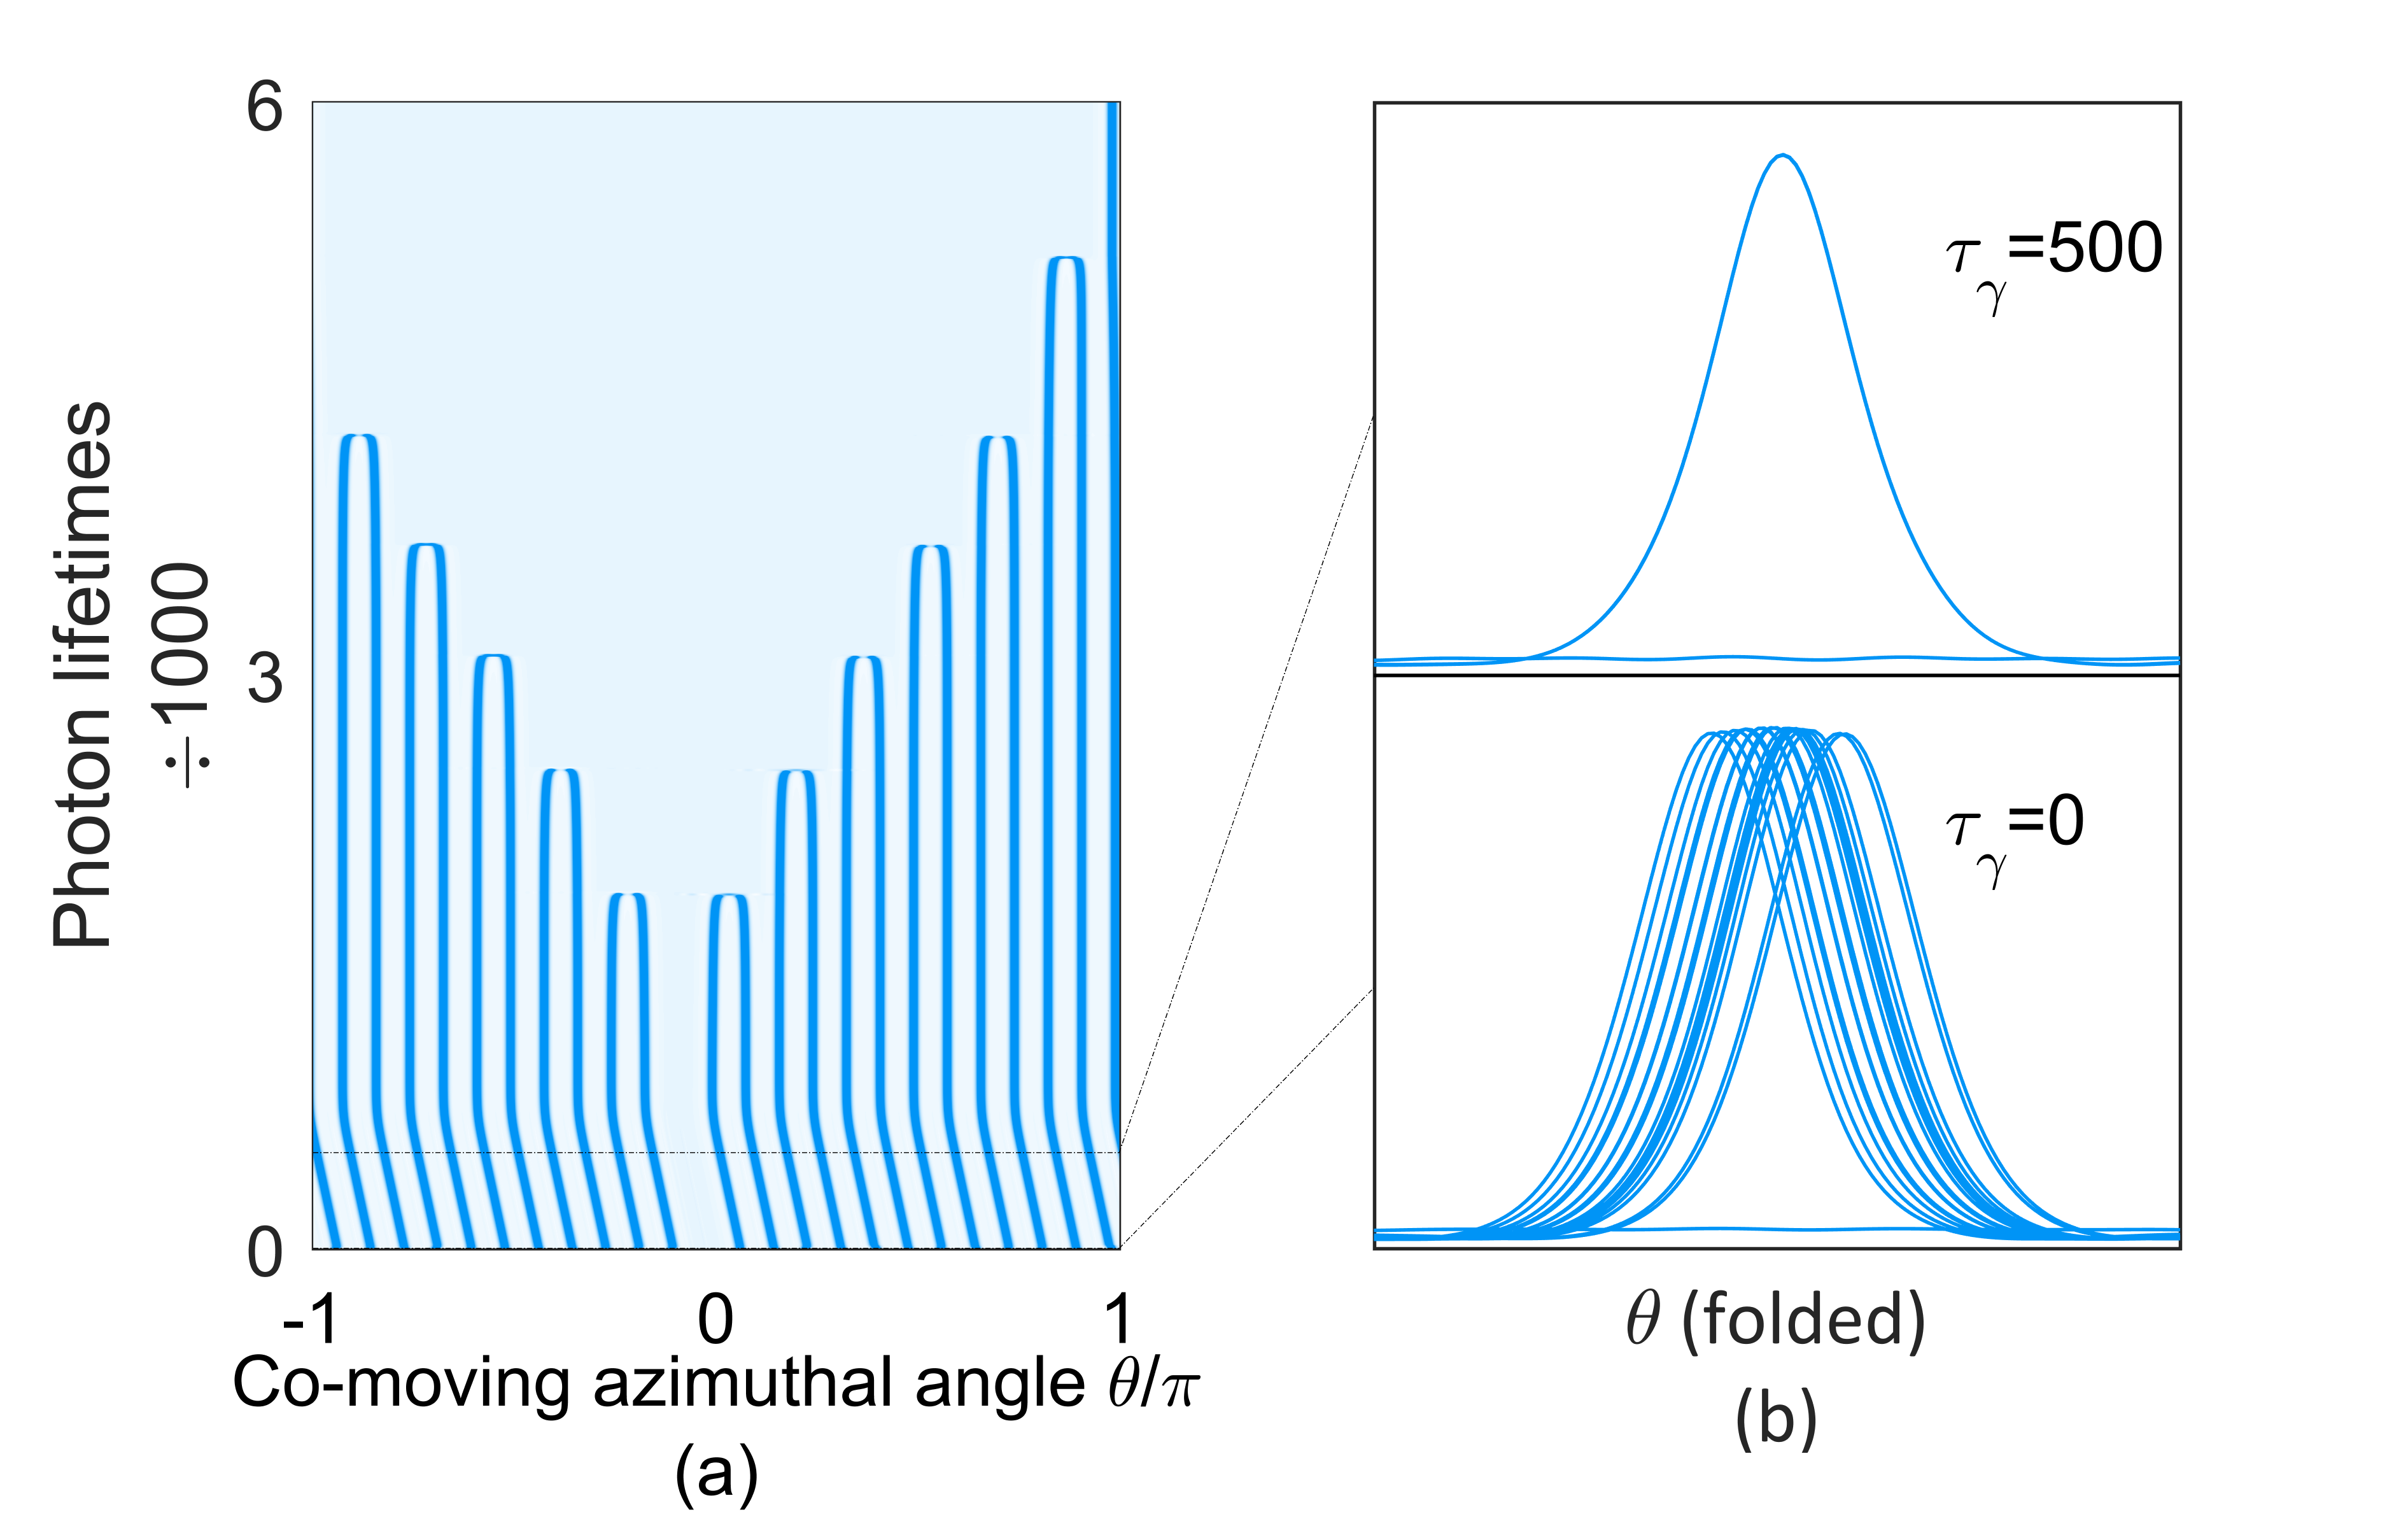
\includegraphics{\FigPath/Figures/SolitonCrystals/SCexamplesim.png}
	\end{center}
	\caption[Stabilization and collapse of a soliton crystal]{\textbf{Stabilization and collapse of a soliton crystal.} (a) Simulated evolution of the pulse train corresponding to the experimental crystal spectrum shown in Fig. \ref{fig:SCexample}c, starting from irregular pulse positions. For the first 500 photon lifetimes of the simulation, the propagation is governed by a perturbed LLE including reduced comb-resonator detuning on modes $\mu_{\times,1}=120$ and $\mu_{\times,2}=168$. The soliton ensemble crystallizes within 10 seconds of initialization of the simulation, and then drifts within the co-rotating frame because the additional CW light on modes $\mu_{\times,1}$ and $\mu_{\times,2}$ corresponds to traveling waves. The reduced comb-resonator detuning is removed smoothly from 500 to 1000 photon lifetimes, resulting in the destabilization of the crystal and pair-wise annihilation of the solitons. (b) Intracavity power with the azimuthal coordinate folded modulo $2\pi/24$, demonstrating the initial irregularity of the pulse positions and the crystallized pulse train after 500 photon lifetimes.}
	\label{fig:SCexamplesim}
\end{figure} 


\section{Case study: pair distribution function for a superstructured crystal}

We consider a third specific example of a soliton crystal. The measured and simulated optical spectra for this crystal are shown in Fig. \ref{fig:SCsuperstructure}a. This crystal exhibits superstructure---the soliton pulse train is nearly periodic in a small unit cell but is modulated with a larger periodicity. This results from the frustrated uniform distribution of 16 solitons with allowed inter-soliton separations of $2\pi n/49$ radians; one pair is spaced by $4 \times 2\pi/49$ instead of $3 \times 2\pi/49$ radians.  Excess power is apparent in the spectrum at mode $\mu_\times=49$ (highlighted by the red circle in the plot), and we simulate this crystal phenomenologically by reducing the comb-resonator detuning on mode 49 so that the observed and simulated amplitudes of this mode agree. The total background wave that emerges as the sum of the waves from each constitutent soliton, is visible in the plots of the simulated intensity in Fig. \ref{fig:SCsuperstructure}b and c.

\begin{figure}[htpb]
	\begin{center}
		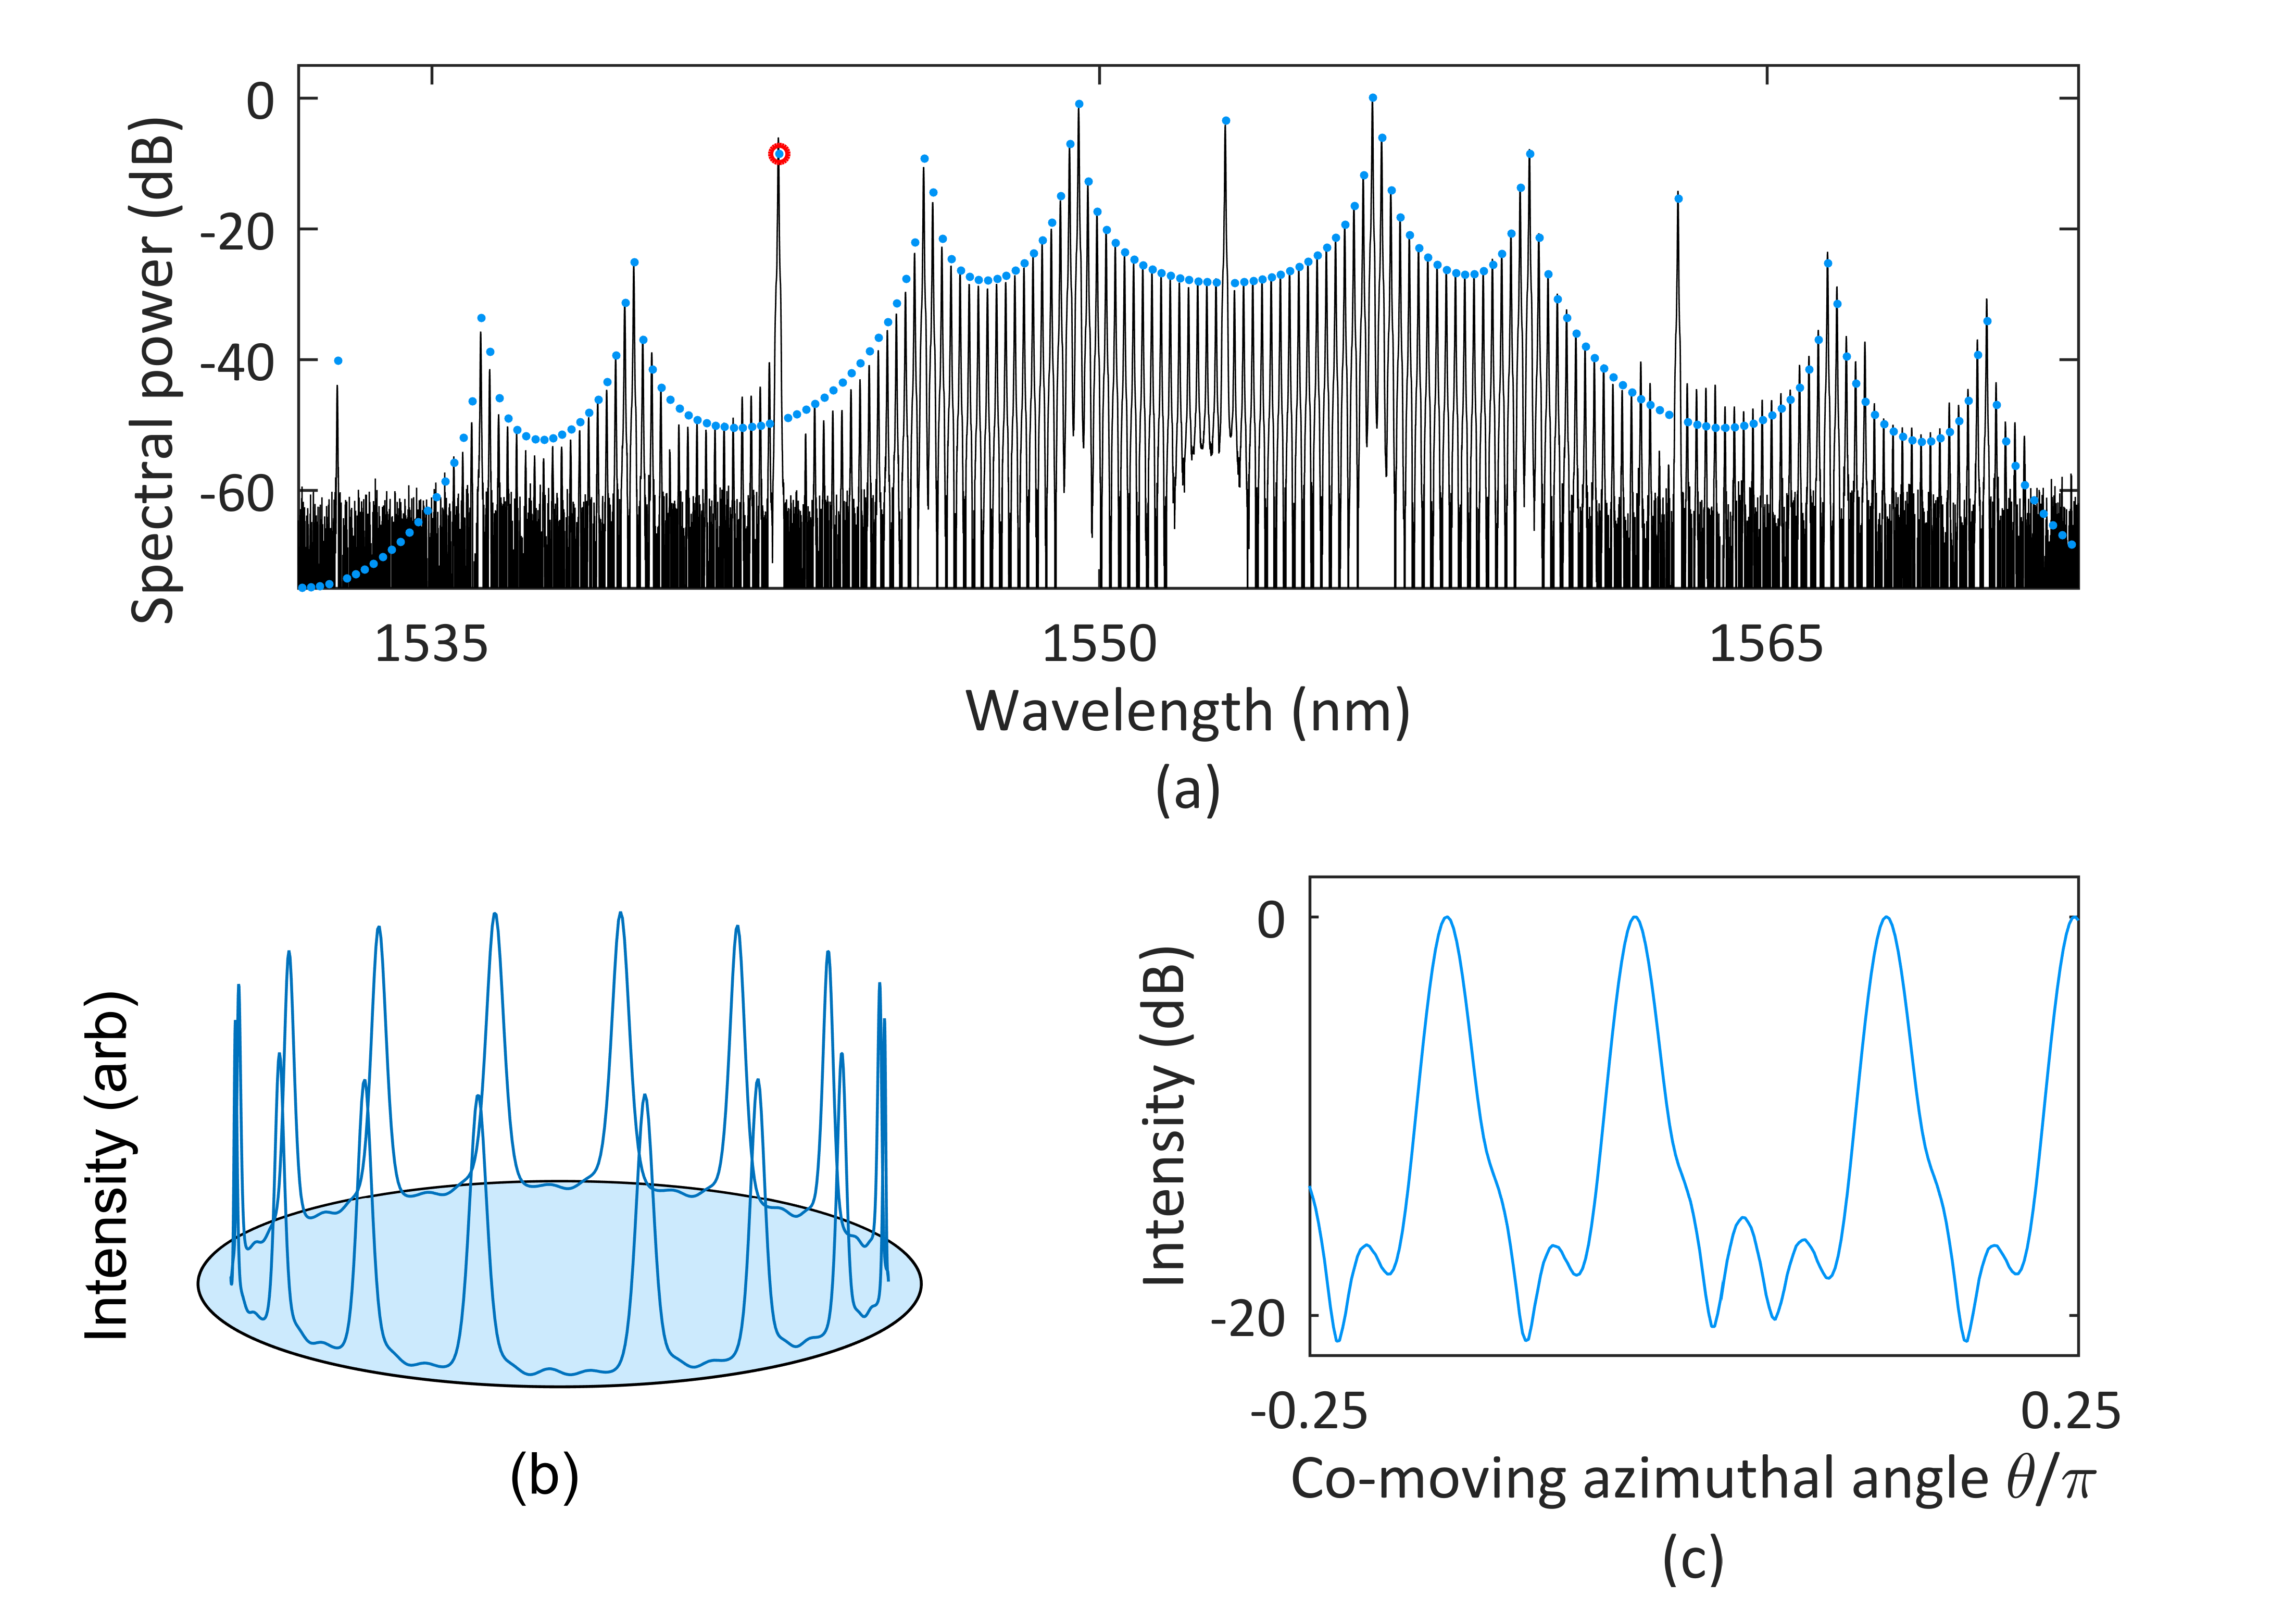
\includegraphics{\FigPath/Figures/SolitonCrystals/SCsuperstructure.png}
	\end{center}
	\caption[Spectrum and waveform of a superstructed soliton crystal]{\textbf{Spectrum and waveform of a superstructured soliton crystal.} (a) Experimental (black) and simulated (blue) optical spectra of a superstructured crystal, with the red dot indicating the mode affected by a mode crossing as described in the text. (b) Simulated time-domain intensity of frustrated-uniform distribution of 16 solitons over 49 lattice points. (c) Zoomed-in logarithm-scale plot of the same that clearly shows unoccupied lattice sites and the anomalous $4\times2\pi/49$ spacing between a pair of pulses.}
	\label{fig:SCsuperstructure}
\end{figure} 

To gain insight into crystal generation, we simulate laser frequency scans across the resonance that generate this crystal in the presence of the mode crossing on mode 49. Example scans are shown for the case without the mode crossing (green) and with it (blue) in Fig. \ref{fig:SCsimgen}. In both scans, solitons emerge from chaos as the frequency of the laser is decreased. In the presence of the mode crossing, they are generated with inter-soliton separations of $2\pi n/49$ radians. A greater number of solitons emerge from chaos in the presence of the mode crossing, and this is consistent with the observed thermal stability of crystal generation in the experiment. Upon continuation of the simulation, some of the solitons in the scan without the mode crossing interact attractively and pair-annihilate, while the crystallized ensemble resulting from the scan with the mode crossing remains stable indefinitely.

\begin{figure}[htpb]
	\begin{center}
		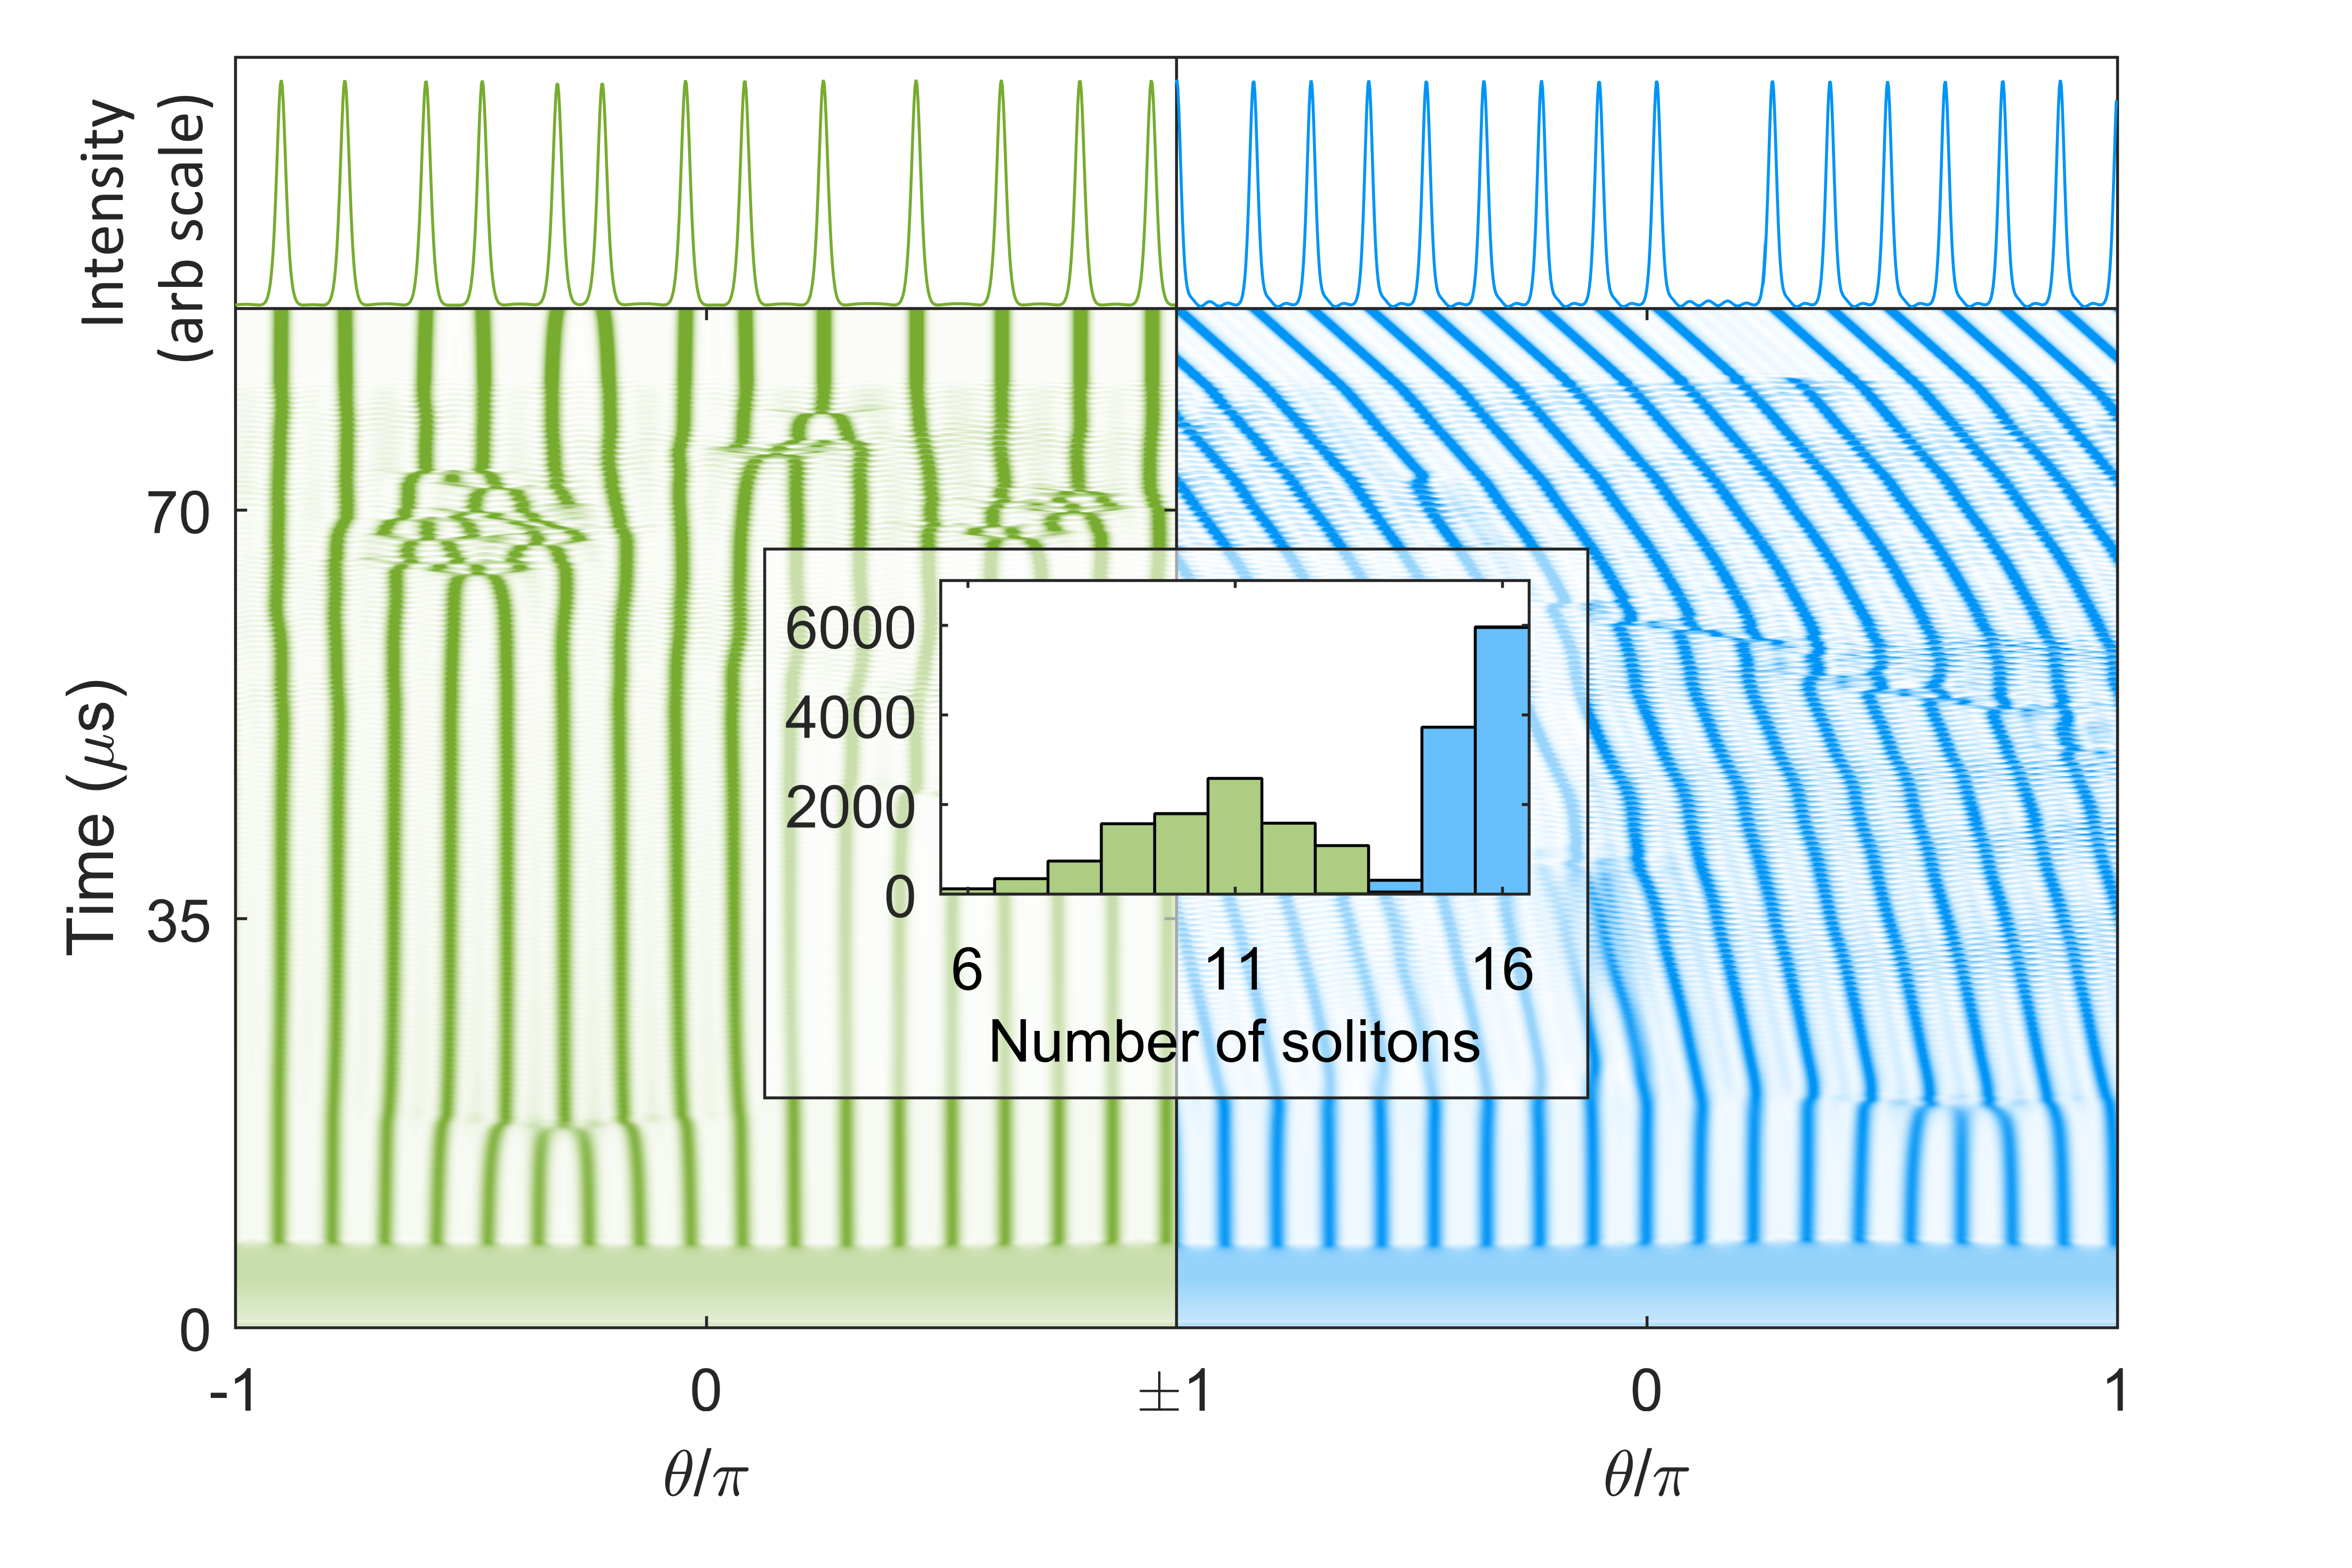
\includegraphics{\FigPath/Figures/SolitonCrystals/SCsimgen.png}
	\end{center}
	\caption[Simulated generation of a superstructured soliton crystal]{\textbf{Simulated generation of a superstructured soliton crystal.} Bottom: plots of the intracavity power during a simulated scan across the resonance, without (green) and with (blue) a mode crossing on mode 49 that reduces the comb-resonator detuning and increases the efficiency of frequency conversion on that mode. Top: final waveforms. Inset: histogram of the number of solitons generated in 10,000 simulated scans.}
	\label{fig:SCsimgen}
\end{figure} 

We investigate the pair distribution function (PDF) for the soliton ensembles generated by these scans. The PDF is the probability that a soliton exists at position $\theta_0+\Delta\theta$ given that a different soliton exists at position $\theta_0$, normalized to the density. This is a useful metric to classify particle interactions that we borrow from condensed matter physics (see e.g. Ref. \cite{Barker1976}, especially Fig. 2, and Ref. \cite{Egami2012}, especially Fig. 1.1 and Chapter 3). We note that for numerically calculated discrete PDFs the absolute scaling of the PDF is not important, as it depends on the density of numerical sampling. In Fig. \ref{fig:SCpdf}, we plot the average PDFs for 10000 simulated scans with and without the mode crossing. The result for the case with a mode crossing is sharply peaked, indicating that the allowed inter-soliton separations take on discrete values. The result for the case without the mode crossing is continuous, with a peak near the most likely nearest-neighbour separation and periodic revivals at its multiples, falling to the value of the PDF for uncorrelated soliton positions (the density) at large separations. This is exactly the expected form of the PDF for a liquid \cite{Barker1976,Egami2012}. For comparison, we plot a PDF (black) generated by simulation of a simple particle ensemble with mean inter-particle separation of $\Delta\theta=0.155\pi$ and normally distributed noise on this value with standard deviation of $\sigma_{\delta\theta}=0.18\Delta\theta$. Thus, with a particle labeled by $n = 0$ fixed at $\theta = 0$, the position of particle $n$ is $\theta_0 = n\Delta\theta + \Sigma_n\delta\theta_i$, with $\delta\theta_i$ the instantiations of the random variable representing the noise on the pulse spacings. This simple model qualitatively matches the observed PDF for the simulations without the mode crossing.

\begin{figure}[htpb]
	\begin{center}
		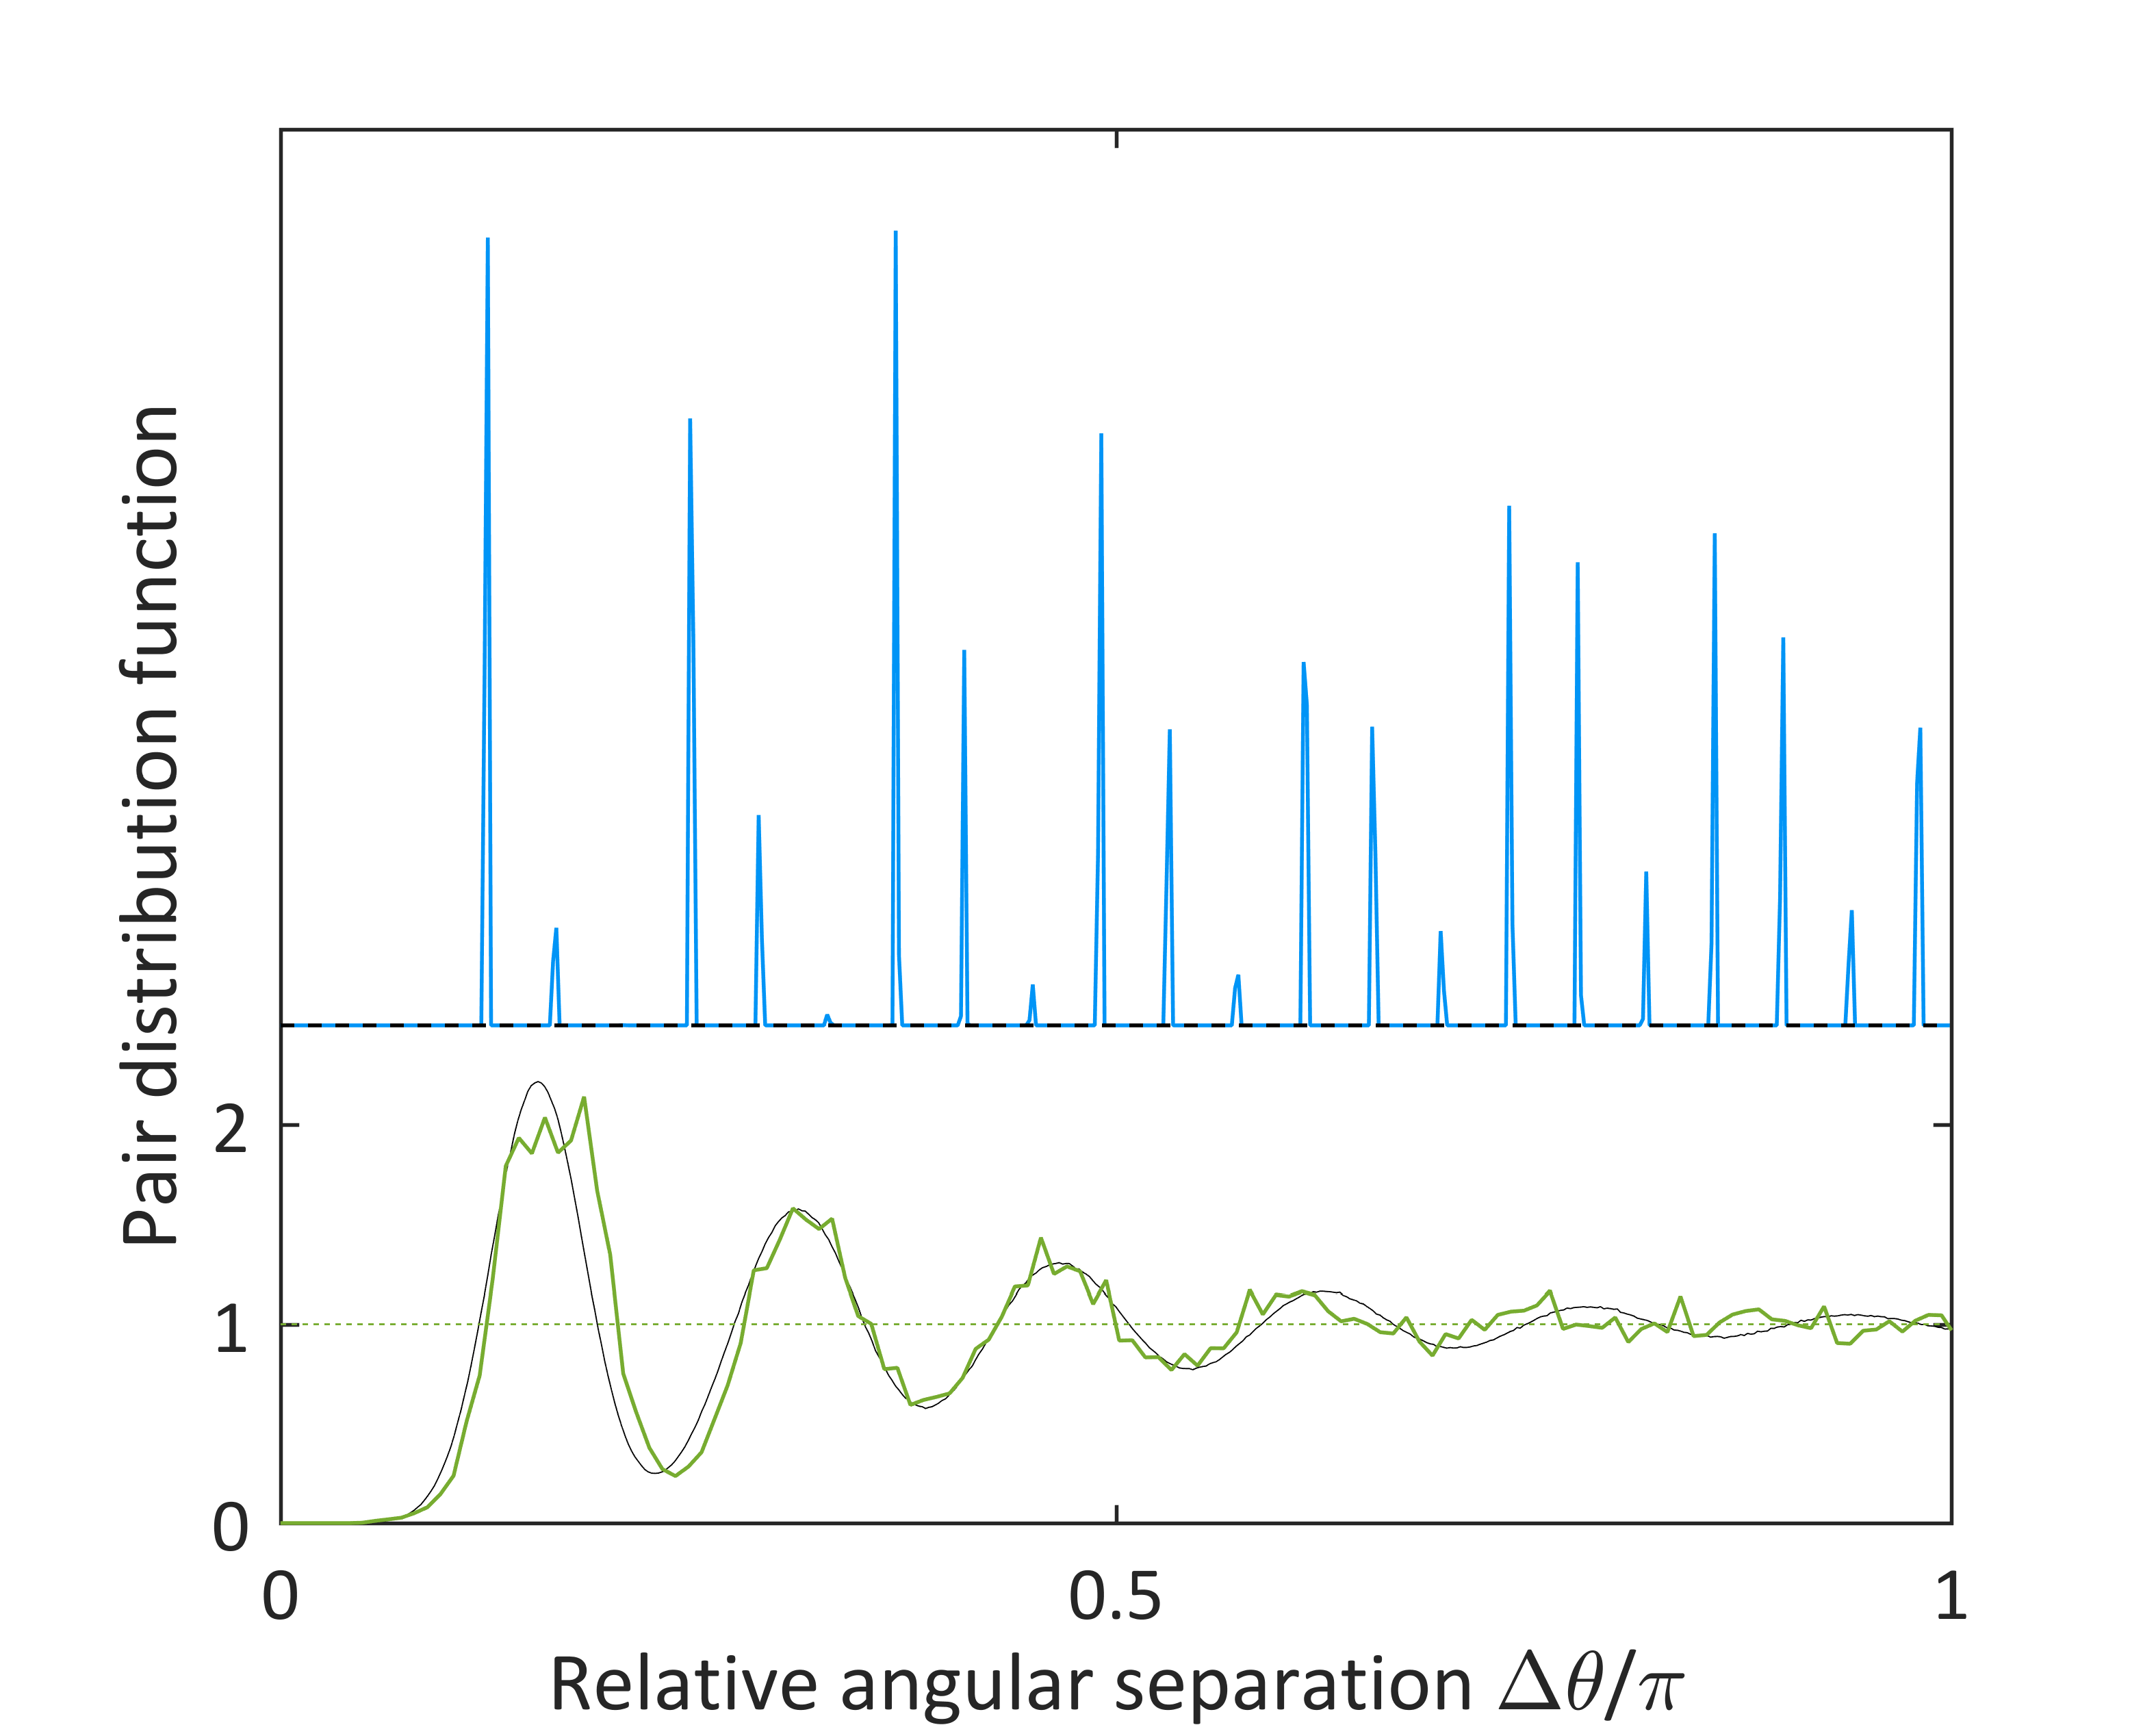
\includegraphics{\FigPath/Figures/SolitonCrystals/SCpdf.png}
	\end{center}
	\caption[Pair distribution function for soliton crystal generation]{\textbf{Pair distribution function for soliton crystal generation.} Average pair distribution functions calculated over 10,000 simulated scans across the resonance with (blue) and without (green) a mode crossing on mode 49. The width of the peaks in the discrete PDF is a single $\Delta\theta$ bin. The expected PDF of a simple one-dimensional soliton liquid (see main text) is plotted for comparison in black.}
	\label{fig:SCpdf}
\end{figure} 


 
\section{Soliton crystal configuration space}\label{sec:SCtaxonomy}

We observe a rich variety of soliton crystals explained by ordering in accordance with an extended background wave as described above. Operationally, we adjust the pump laser power to provide repeatable conditions for creating particular crystals; crystals exhibiting a greater number and variety of defects occur with increased laser power, which intensifies the fluctuations in the chaos that precedes crystal generation and provides less well-ordered initial conditions. Once a crystal is generated, it is stable to small adjustments in the pump power and detuning in accordance with the range of soliton existence shown in Fig. \ref{fig:MRLLEspace}, as the crystal structure is determined by the initial conditions for soliton formation rather than by an explicit dependence on pump power or detuning. 

Our interpretation of experimental data is based first on the fact that the LLE restricts the behavior of the field $\psi$ to either an extended pattern (primary comb pulse train or chaos) or an ensemble of solitons. Simultaneous experimental measurement of 1. A quiet repetition-rate tone when the spectrum of the photodetected power is analyzed, and 2. Single-FSR spacing in the power spectrum indicate that a Kerr-comb is a soliton crystal\footnote{These requirements are probably sufficient, but not necessary---for example, a defect-free crystal will exhibit multi-FSR spacing. Experimentally, the difference between such a crystal and a primary-comb pulse train lies in the parameters $\alpha$ and $F^2$ that place the pump laser \textit{either} in the regime for solitons or the regime for primary comb. However, these parameters are not necessarily straightforward to determine.}. To determine the temporal structure of a soliton crystal, we begin with the assumption that the spectrum corresponds to a soliton ensemble. Using the properties of the Fourier transform (e.g. linear superposition and the fact that a shift in time corresponds to a linear spectral phase shift), it is usually possible to deduce the configuration of pulses that must lead to the observed spectrum. Once the pulse train corresponding to the general structure of the spectrum has been deduced, the experimental spectrum can be compared to the spectrum of this pulse train calculated as an ensemble of solitons according to Eq. \ref{eq:LLEsolens}. This comparison reveals localized excess power in the experimental spectrum, which is evidence of a mode crossing. The strength of the mode crossing, controlled in the experiment by e.g. the taper-induced coupling between modes, is determined phenomenologically from the magnitude of the excess power and reduced comb-resonator detuning on a single mode is incorporated into a perturbed LLE as described in Sec. \ref{sec:crystallizationmechanism}. It is then verified that the pulse train whose spectrum matches the experimental data is a steady-state solution to this perturbed LLE, which requires the inter-soliton separations to be multiples of the period of the beat between the excess power and the pump laser. This period is $2\pi /\mu_\times$, where $\mu_\times$ is the mode number of the affected mode. Because this process connects the presence of excess power on a single optical mode of the Kerr-comb spectrum to the general shape of the spectrum, two observations that are not related a priori, it provides strong evidence that the time-domain waveform of the crystal has been determined correctly.

The crystals we observe exhibit vacancies (Schottky defects), dislocations (Frenkel defects), disorder, or superstructure, or some combination thereof \cite{Ashcroft1976}. In a disordered crystal, the solitons still occupy lattice sites whose positions are determined by an avoided mode crossing in the resonator spectrum, but their distribution over these lattice sites varies without any apparent regular order or favored period. In this case, it is less straightforward to determine the pulse configuration from the shape of the spectrum. Instead, to determine the pulse configuration for a disordered crystal, we first identify excess power due to a mode crossing through observation of an asymmetry in the spectrum about the pump. The location of the excess power then fixes the allowed inter-soliton separations in the resonator, after which an exhaustive search is performed until a pulse train is found that yields the experimental spectrum. 

\begin{sidewaysfigure}[htpb]
	\begin{center}
		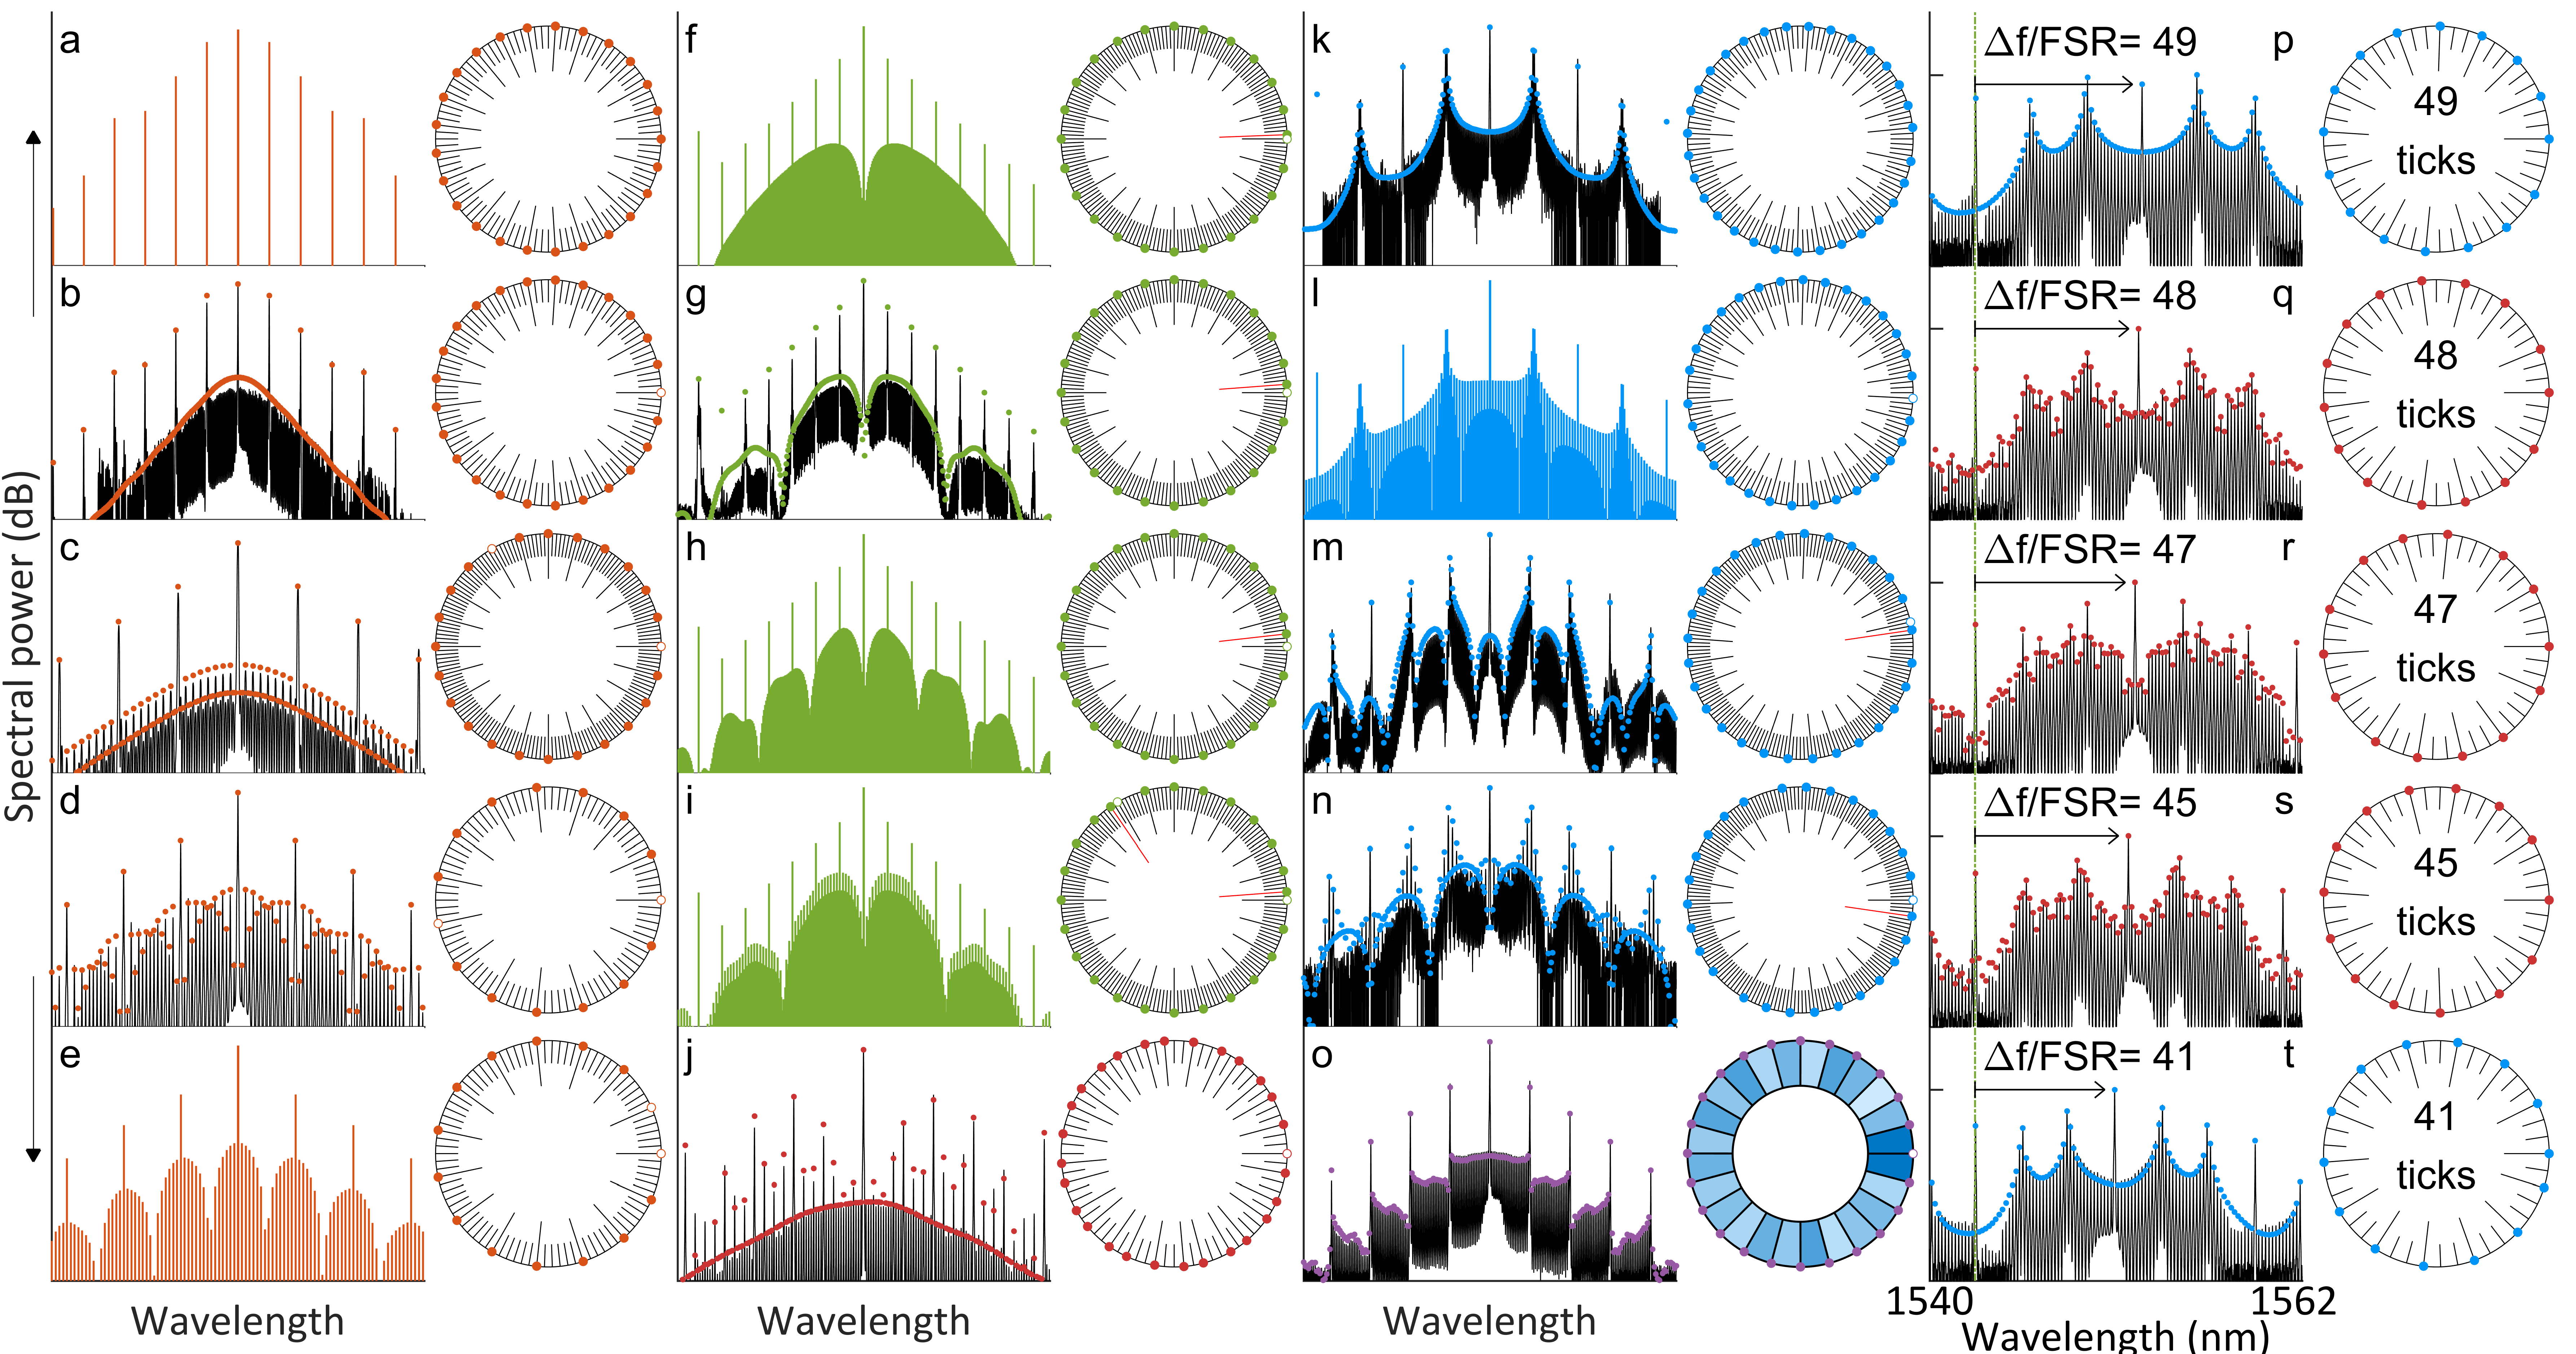
\includegraphics{\FigPath/Figures/SolitonCrystals/SCtaxonomy.png}
	\end{center}
	\caption[Taxonomy of soliton crystals]{\textbf{Taxonomy of soliton crystals.} Measured optical spectra are shown in black, with simulations in color. Schematic depictions of the soliton distribution in the resonator co-moving frame are shown to the right of each spectrum. Major ticks in the schematic diagrams indicate the location or expected location of a soliton. Minor ticks indicate lattice sites, corresponding to peaks of the extended background wave due to a mode crossing. (a) A perfect soliton crystal, consisting of 25 uniformly-distributed solitons. (b-e) Soliton crystals exhibiting vacancies. (f-i) Soliton crystals exhibiting Frenkel defects. Shifted solitons still occupy a lattice site. (j) A disordered crystal. (k-n) Crystals exhibiting superstructure. (o) A crystal with irregular inter-soliton spacings. Darker shading indicates a smaller inter-soliton spacing. The range in inter-soliton spacings is 3 $\%$ of the mean. (p-t) A series of crystals generated as the pump laser is moved progressively closer to the stabilizing mode crossing.}
	\label{fig:SCtaxonomy}
\end{sidewaysfigure}


Optical spectra for various observed and hypothetical soliton crystals are plotted in Fig. \ref{fig:SCtaxonomy}. We have simulated 13 of the experimental spectra as steady-state solutions to a perturbed LLE (this excludes crystal o); for 10 of these, the stabilizing mode crossing is visible in the data but not necessarily shown in the figure. For the other three the position of the mode crossing is inferred from the distribution of solitons and other crystal states observed in the same resonator.


We highlight the crystal plotted in Fig. \ref{fig:SCtaxonomy}n. This crystal exhibits both superstructure, with a superlattice period of $2\pi/3$ radians, and a Frenkel defect. Three identical supercells per resonator round-trip yield a spectrum which has light in optical modes spaced by three resonator FSR, because the waveform's period has been reduced threefold. The Frenkel defect, occurring once per round-trip, transfers a pulse from one supercell to another and contributes the single-FSR lobes to the spectrum. The result is three bursts of pulses containing 8, 9, and 10 solitons respectively. 	

Fig. \ref{fig:SCtaxonomy}o shows a soliton crystal with inter-soliton separations that are slightly irregular and that we have not simulated as a steady-state solution of any perturbed LLE. We expect that the formation of the crystal and the distribution of solitons are dictated by mode interactions, but that in this case our simple approximation of a perturbation to the LLE by a reduced comb-resonator detuning on a single comb mode is not appropriate.

Finally, we highlight the series of crystals plotted in Figs. \ref{fig:SCtaxonomy}p-\ref{fig:SCtaxonomy}t. This series of crystals was generated by moving the pump laser closer to a mode-crossing in steps of integer multiples of the resonator FSR. This data demonstrates the influence of the background beating between the pump laser and the mode crossing in determining the configuration of solitons in the resonator.





\section{Time-domain measurements of soliton crystals}
It is recognized in ultrafast optics that it is not generally possible to infer the time-domain waveform of an optical signal from its optical power spectrum without additional information \cite{Weiner2009}, because the spectrum contains no phase information. The LLE imposes restrictions on the possible time-domain field behaviors that can be exhibited, which can allow educated guesses to be made about the time-domain field based on the recorded optical spectrum, and we have been successful in modeling the observed spectra presented above as soliton ensembles. However, it is useful to confirm the LLE-assisted interpretation of experimental data both to strengthen the case for the LLE as a useful model for the system and to stay alert to the possibility of extra-LLE phenomena. 

To verify our time-domain interpretation of the spectra we record in experiment, we characterize the temporal intensity of soliton crystals using an optical cross-correlation measurement. A depiction of the approach and the results for measurement of the time-domain intensity of the crystal shown in Fig. \ref{fig:SCtaxonomy}j is shown in Fig. \ref{fig:SCxcorr}. We send the Kerr-comb output and an optical reference pulse train through a LiIO\textsubscript{3} crystal with a relative angle of 90\textsuperscript{o} between the beams. When the beams overlap in the crystal an amount of light proportional to the product of their intensities, at the sum of their frequencies, is emitted in a third direction. By measuring the average power of this emitted light while scanning the relative delay between the two beams, we measure the intensity cross-correlation between the crystal and the reference pulse.

In the limit of a $\delta$-function reference pulse, optical cross-correlation directly measures the time-domain waveform of an unknown signal. To approximate this limit, we perform cross-correlation measurements with a train of reference pulses that have duration comparable to that of the solitons, which allows us to precisely characterize soliton crystals. The reference pulse train is derived through electro-optic modulation (see Chapter \ref{chap:EOMCombs}) from the same laser that pumps the resonator, and the repetition rate of the reference pulse train is locked to the repetition rate of the Kerr-comb output. 

We generate crystals in a through-coupled configuration, which results in interference between the out-coupled solitons and the through-coupled pump that depends on the coupling condition and that effects the time-domain waveform that propagates away from the resonator. In this particular experiment the out-coupled solitons destructively interfere with the through-coupled pump, with the result that the solitons manifest as dips in the through-coupled intensity. To correct this, before cross-correlation we use a spatial light modulator to rotate the phase of the pump laser by $\pi$ so that it constructively interferes with the solitons, yielding solitons riding on top of a CW background. 



\begin{figure}[htpb]
	\begin{center}
		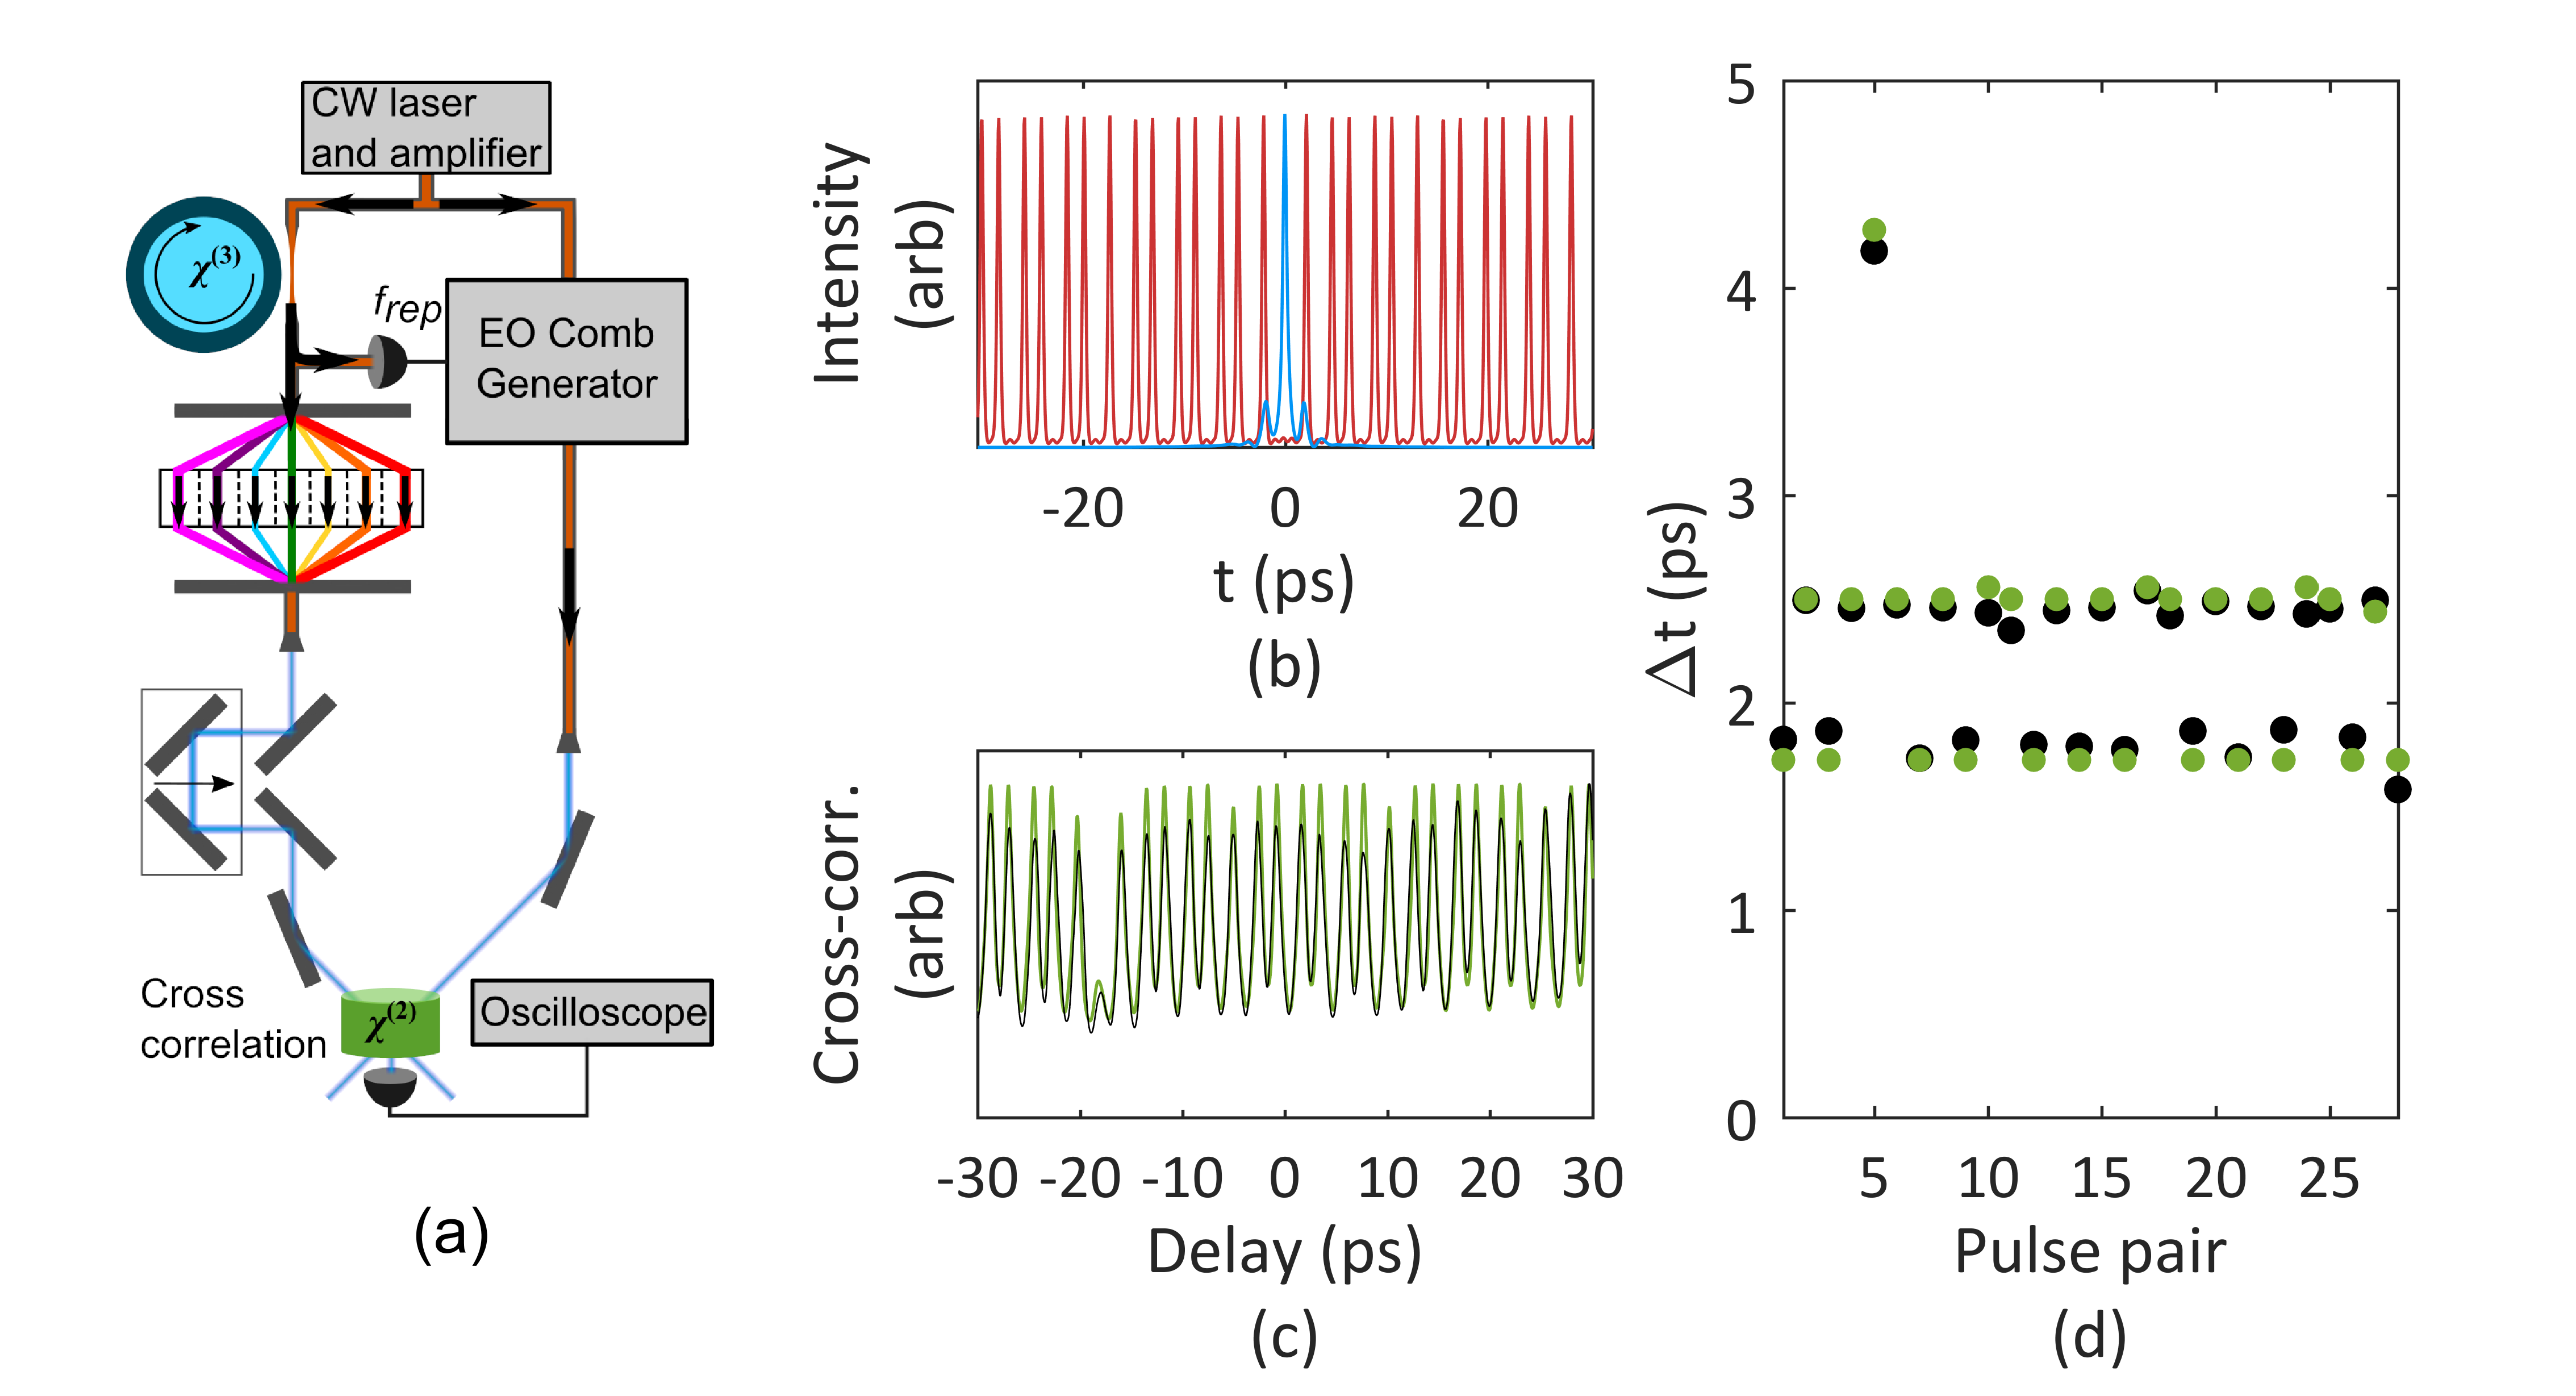
\includegraphics{\FigPath/Figures/SolitonCrystals/SCxcorr.png}
	\end{center}
	\caption[Cross-correlation characterization of a soliton crystal]{\textbf{Cross-correlation characterization of a soliton crystal.} Schematic depiction of the setup for using an electro-optic (EO) modulator comb as a reference pulse to measure the time-domain waveform of a soliton crystal. The $\chi^{(3)}$ (Kerr) and $\chi^{(2)}$ nonlinearities are indicated on the resonator and nonlinear crystal (LiIO\textsubscript{3}). A spatial light modulator is used to rotate the phase of the pump laser by $\pi$ after crystal generation to compensate for interference between the out-coupled soliton crystal and the through-coupled pump light. The soliton crystal and the EO modulator comb share a pump laser, and the repetition frequency $f_{rep}$ of the EOM comb is locked to that of the crystal. Varying the relative delay in one arm of this interferometer enables measurement of the intensity cross-correlation between the soliton crystal and the reference pulse. (b)  Simulated crystal (red) and reference (blue) intensity profiles. (c) Measured (black) and simulated (green) cross-correlation signals. The contrast between peaks of the cross-correlation signal, for both theory and experiment, is limited by the duration and shape of the reference pulse and increases between soliton pairs with larger temporal separations. (d) Temporal separations between adjacent peaks for the measured (black) and simulated (green) cross-correlation signals. Mean fractional error is 3.5~$\%$.}
	\label{fig:SCxcorr}
\end{figure} 

 
The cross-correlation of the disordered crystal shown in Fig. \ref{fig:SCtaxonomy}j with the reference pulse train confirms our interpretation of the spectral data for this crystal. Fig. \ref{fig:SCxcorr}b shows the simulated time-domain waveforms of the reference pulse and the crystal, and Fig. \ref{fig:SCxcorr}c shows measured and simulated cross-correlation signals. The temporal spacing between the peaks of the cross-correlation signals is shown in Fig. \ref{fig:SCxcorr}d, where a high degree of agreement between the data and the simulation is observed. 

The simulated cross-correlation signal is sensitive to the intensity profile of the reference pulse. We can measure only its intensity autocorrelation, which we combine with our knowledge of its production to estimate the intensity profile. To demonstrate that the validity of the results we present here is not sensitive to the exact assumptions we make about the intensity profile, we have also simulated the intensity cross-correlation resulting from an assumed Gaussian reference pulse with the same autocorrelation width as is measured for the reference pulse. The resulting simulated cross-correlation does not qualitatively agree as well with the experimental data in the depths of the wells between peaks because it does not contain satellite pulses which contribute to the variations in this depth, but the quantitative comparison of the temporal spacing between peaks is similar: the mean (maximum) normalized error between experiment and theory is 3.5 $\%$ (9.1 $\%$) for the assumed electro-optic comb pulse and 4.8 $\%$ (10.6 $\%$) for the Gaussian pulse.







% \chapter{Theory of Kerr frequency combs in Fabry-Perot resonators} \label{chap:FPLLE}

Generation of Kerr frequency combs in the ring-resonator geometry appears quite promising for applications. However, a second possibility is to use the same processes for comb generation, but with a Fabry-Perot (FP) resonator geometry. The FP geometry offers a new degree of freedom relative to the ring resonator, which is the possibility to employ chirped mirrors, mirror coatings, or distributed Bragg reflectors, and therefore exert greater control over the total cavity dispersion. Other differences with the ring geometry may ultimately prove important, for example the smaller footprint possible in a cavity of total length $L$ with the FP geometry versus the ring geometry could allow for denser and more flexible integration of Kerr combs in photonics systems. Kerr-comb generation in an FP cavity using a pulsed pump laser was recently described in Ref. \cite{Obrzud2017}.

In this chapter we present a brief theoretical investigation of the difference in the nonlinear dynamics that occur in a Kerr-nonlinear FP resonator versus a Kerr-nonlinear ring resonator. Our starting point is the Fabry-Perot Lugiato-Lefever equation (FP-LLE), which is derived in detail in Ref. \cite{Cole2018a}, beginning from a set of coupled equations that describe the interaction of the envelopes for the forward- and backward-propagating fields in the cavity with the Kerr medium. A derivation of equivalent coupled mode equations is provided in Ref. \cite{Obrzud2017}. We do not reproduce the derivation of the equation here; our goal is to understand its description of Kerr-comb dynamics. The equation is:
\begin{equation}
\frac{\partial\psi}{\partial\tau}=-(1+i\alpha)\psi+i|\psi|^2\psi-i\frac{\beta_2}{2}\frac{\partial^2\psi}{\partial\theta^2}+2i\psi\left<|\psi|^2\right>+F\label{eq:FPLLE}.
\end{equation}
Here, $<g>$ denotes the spatial average over the domain: $<g>=\frac{1}{2\pi}\int_{-\pi}^{\pi}d\theta\,g(\theta)$. This equation is identical to the LLE for the ring cavity except for the term $2i\psi\left<|\psi|^2\right>$ describing modulation by twice the average of the intracavity power. The coordinate $\theta$ is defined as $\theta=2\pi z/2L$, where $z$ is a co-moving longitudinal coordinate (so that, for example, solitons are stationary functions of $\theta$) on a domain $-L\leq z\leq L$; $L$ is the physical length of the Fabry-Perot cavity. The time $\tau$ is once again normalized to twice the photon lifetime $\tau_\gamma$: $\tau=t/2\tau_\gamma$. The normalized experimental parameters in the FP-LLE are the same as in the LLE for the ring cavity, with $\alpha$ the detuning, $\beta_2$ the dispersion, and $F^2$ the pump power:
\begin{equation}
\alpha=-\frac{2(\omega_o-\omega_c)}{\Delta\omega_o},
\end{equation}
\begin{equation}
\beta_2=\left.-\frac{2D_2}{\Delta\omega_{tot}}=-\frac{2}{\Delta\omega_o}\frac{\partial^2\omega_\mu}{\partial \mu^2}\right|_{\mu=0}, \label{betaLLE}
\end{equation}
\begin{equation}
F^2=\frac{8g_o\Delta\omega_{ext}}{\Delta\omega_{tot}^3}\frac{A_{eff}}{A_{in}}\frac{n_o}{n_{ext}}\frac{P}{\hbar\omega_o}.
\end{equation}
In the above, $\omega_\mu$ represents the set of resonance frequencies of the cavity including the effects of dispersion, with $\mu=0$ indexing the pumped mode (see e.g. Ref.~\cite{Brasch2016}). The cavity loss and coupling rates $\Delta\omega_{tot}$ and $\Delta\omega_{ext}$ are related to the mirror reflectivity $R$ and transmission $T$ via $\Delta\omega_{tot}=(1-R)c/n_gL$ (where two identical mirrors are assumed) and $\Delta\omega_{ext}=cT/2n_gL$, with $n_g=c/v_g$ the group index. The quantities $A_{in}$ and $A_{eff}$ represent the mode's effective area $\pi w_{in}^2$ (for a Gaussian mode of radius $w$) at the input mirror and the same averaged over the cavity of length $L$, $\frac{\pi}{L}\int dz\, w(z)^2$, respectively. Further, $g_o=n_2\hbar\omega_o^2 D_1/(2\pi n_g A_{eff})$ is the nonlinear gain parameter, where $D_1=\left.\frac{\partial\omega_\mu}{\partial \mu}\right|_{\mu=0}$ is the cavity free-spectral range in angular frequency (here and in Eq.~(\ref{betaLLE}) $\mu$ is treated as a continuous variable). The nonlinear index $n_2$ is related to the third-order susceptibility via $\chi^{(3)}=(4/3)n_o^2\epsilon_ocn_2$, where $n_o$ is the refractive index of the nonlinear medium.  The power $P=\eta P_{inc}$ denotes the mode-matched power, with mode-matching factor $\eta$ and power $P_{inc}$ incident on the input mirror, and $n_{ext}$ is the refractive index of the medium external to the cavity. 

\begin{figure}[htpb]
	\begin{center}
		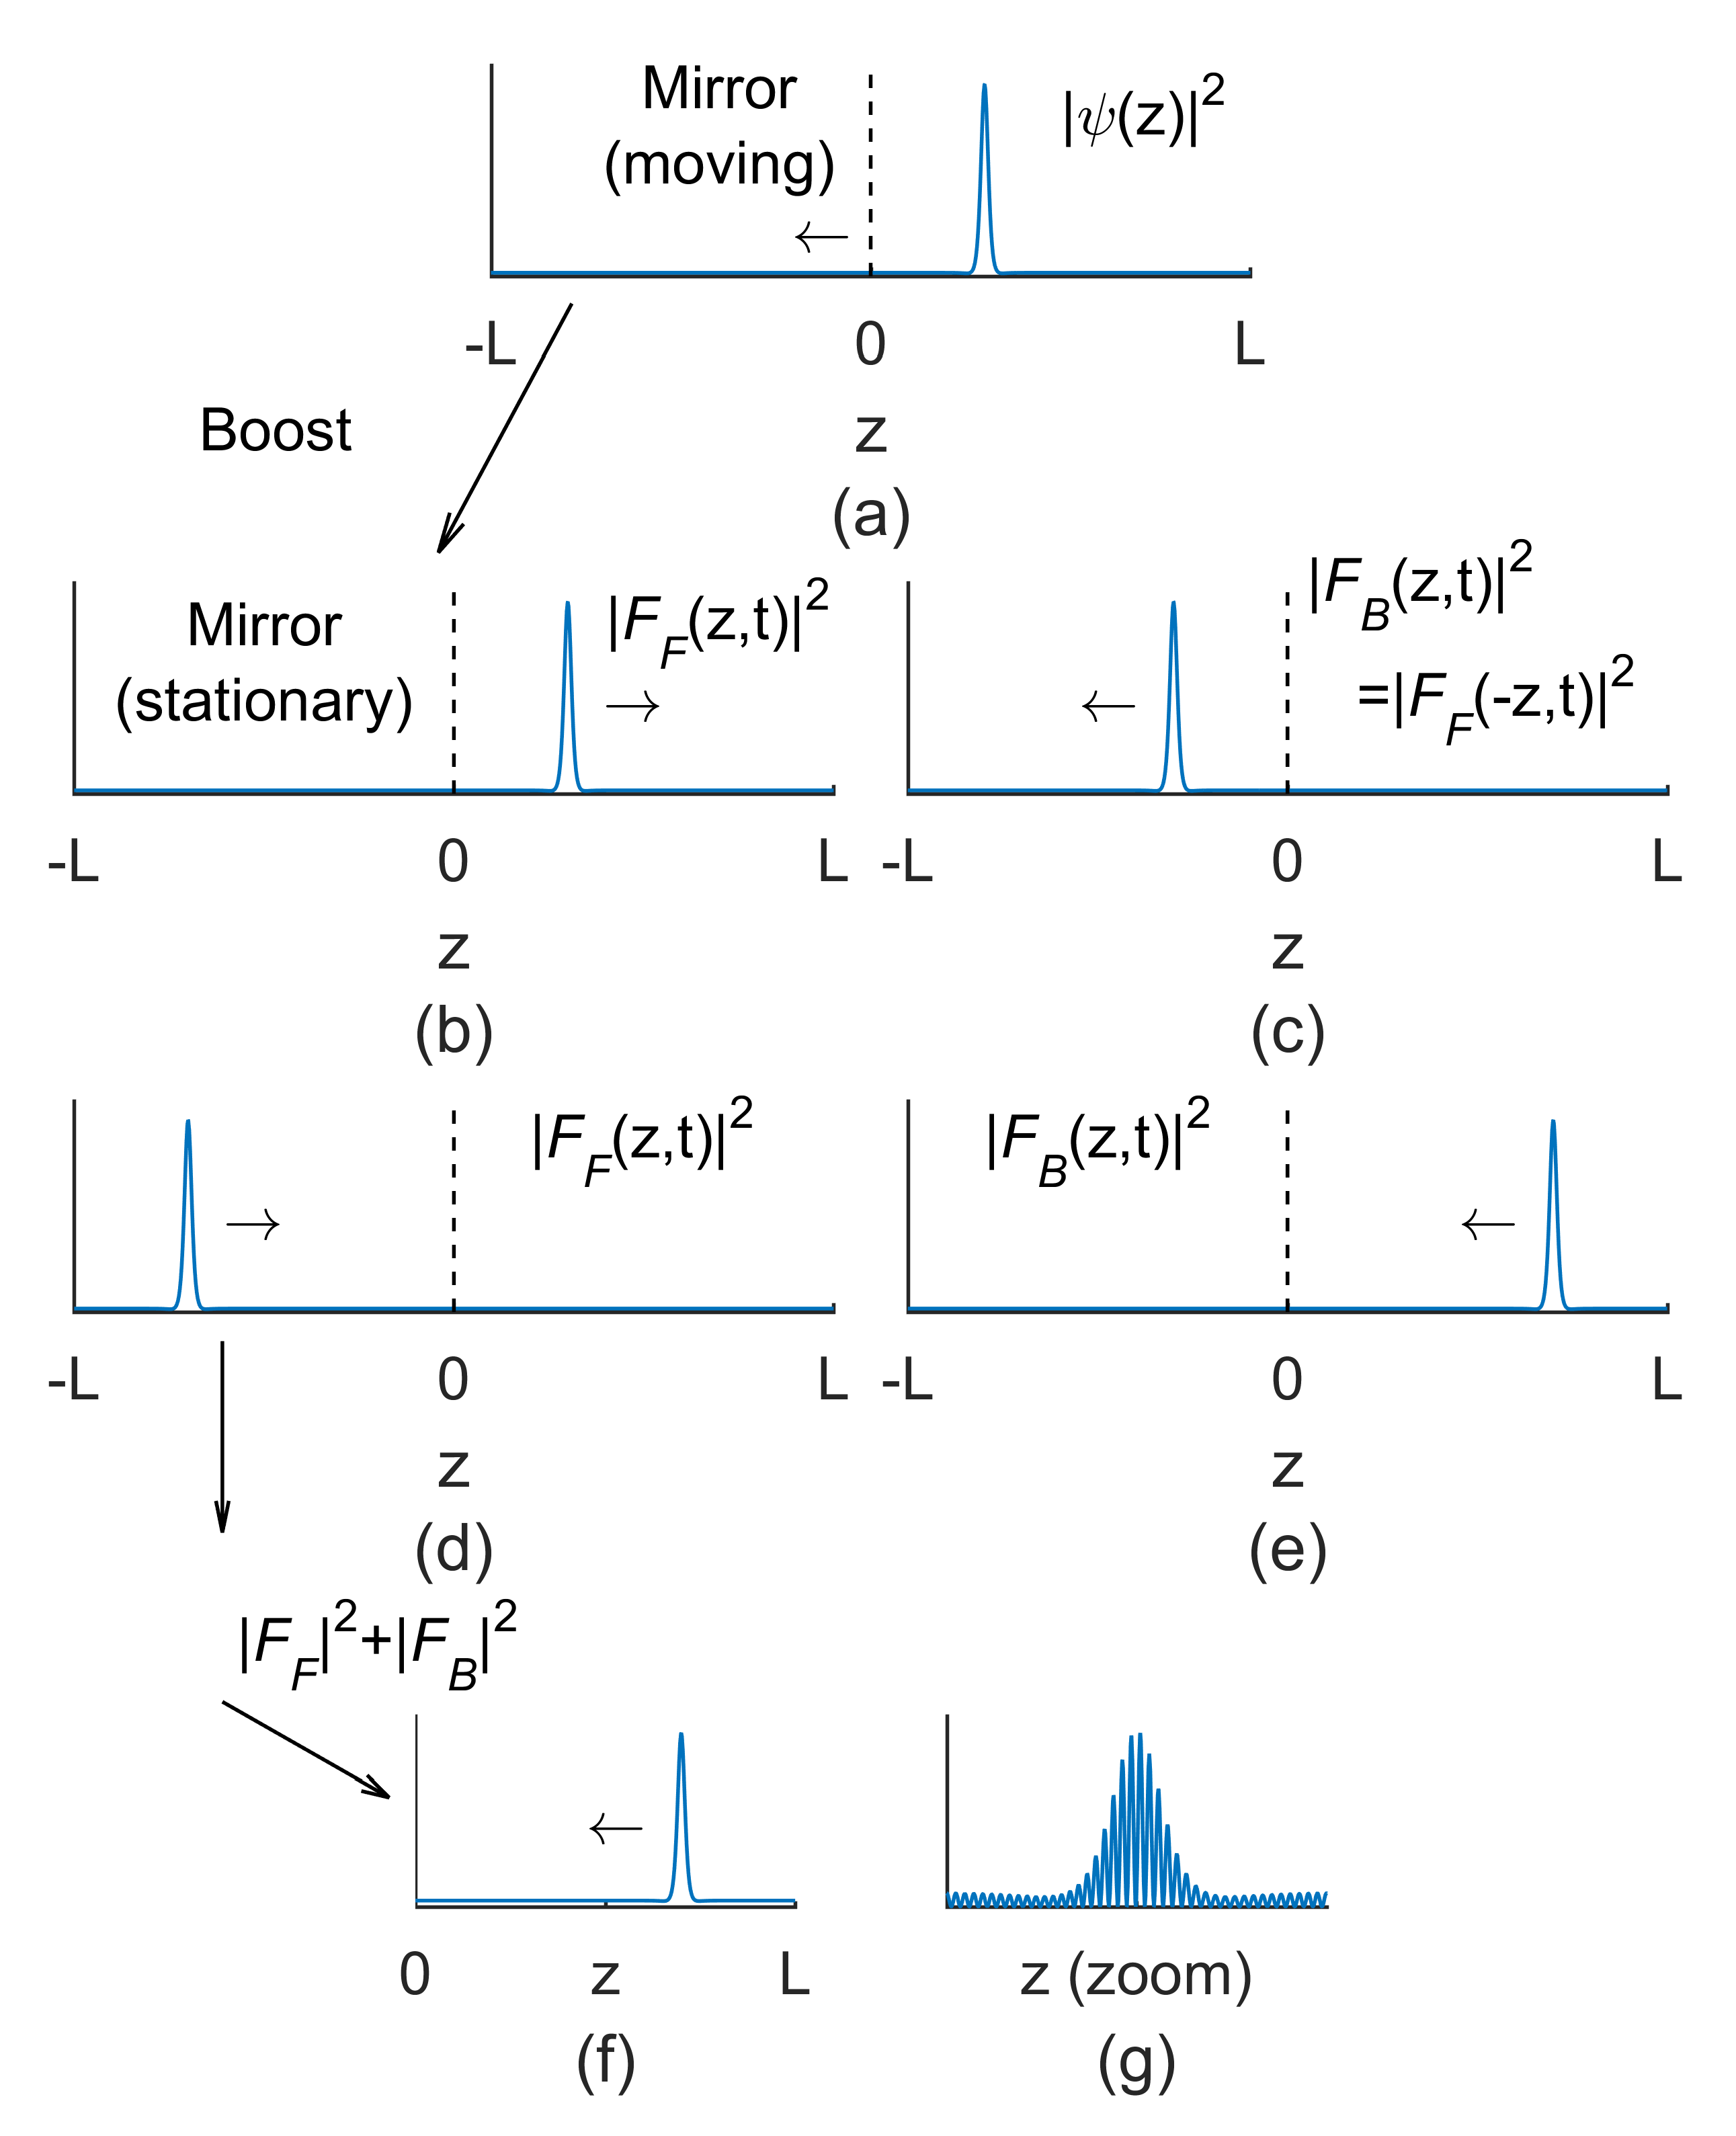
\includegraphics[]{\FigPath/Figures/FPLLE/FPLLEfieldconstruction.png}
	\end{center}
	\caption[Relationship between the physical field in the Fabry-Perot cavity and the co-moving field $\psi$]{\textbf{Relationship between the physical field in the Fabry-Perot cavity and the co-moving field $\psi$.} (a) A soliton stationary solution to the FP-LLE in the co-moving domain of length $2L$, in which the physical components of the cavity (e.g. mirror) move. (b) Intensity of the field $F_F$ in the lab frame, in which the cavity is stationary. (c) Intensity of $F_B$ in the lab frame, related to $F_F$ by reflection about the origin. (d,e) Depictions of the same after propagation for half of the cavity round-trip time. (f) Total intensity of the field on the physical domain $0 \leq z \leq L$. (g) The intensity of the field including the background standing wave that results multiplication of $F_F$ and $F_B$ by the appropriate traveling waves. }
	\label{fig:FPLLEfieldconstruction}
\end{figure} 

The formulation of the FP-LLE in terms of the field $\psi$ defined in the co-moving domain of length $2L$ facilitates numerical simulation of the nonlinear dynamics. To obtain the physical, propagating field in the Fabry-Perot cavity, the arguments of the field $\psi$ are transformed back to dimensionful parameters so that we have $\psi(z,t)$, and then it is boosted to group velocity $v_g$ in the domain of length $2L$ to obtain $\overline{\psi}$, which propagates with periodic boundary conditions $\overline{\psi}(-L,t)=\overline{\psi}(L,t)$. From $\overline{\psi}(z,t)$ we define functions $F_F$ and $F_B$ that are proportional to the forward-propagating and backward-propagating envelopes of the electric field as $F_F(z,t)\propto\overline{\psi}(z,t)$ and $F_B(z,t)\propto\overline{\psi}(-z,t)$, so that they are related by reflection about $z=0$. The quantity $|F_B(z,t)|^2+|F_F(z,t)|^2$ on the physical domain $0\leq z \leq L$ is then proportional to the intensity in the FP cavity as a function of time, averaged over fast spatial and temporal oscillations associated with the optical frequency. If desired, these can be included by multiplying $F_B$ and $F_F$ by the appropriate traveling waves before summation. This process is depicted schematically in Fig. \ref{fig:FPLLEfieldconstruction}.



In the remainder of this chapter we provide an investigation of the nonlinear dynamics in a Fabry-Perot cavity as they relate to the generation of frequency combs. We will focus here exclusively on the properties of FP solitons, as these have been idenfitied as the most promising route towards meeting application needs with Kerr-combs.

\section{General relationship between the ring LLE and the FP-LLE}
As can be seen from Eq. \ref{eq:FPLLE} for the Fabry-Perot cavity and Eq. \ref{eq:LLE} for the ring cavity, the difference between the two geometries lies in the term in the FP-LLE $2i\psi\left<|\psi|^2\right>$. This term represents the cross-phase modulation of the field $\psi(\theta,\tau)$ at each co-moving point $\theta$ by each other co-moving point $\theta'$ as $\theta$ and $\theta'$ propagate through each other during a round trip of the Fabry Perot cavity. The incorporation of this effect into the FP-LLE as a spatial average is consistent with the inclusion of the drive $F$ and out-coupling $\Delta\omega_{ext}$ (which is included in the damping term $\partial\psi/\partial\tau=-\psi...$) into the LLE as delocalized, constant operators; this approximation is valid for high-finesse cavities, in which the field $\psi$ changes little on the timescale of a round trip.

We can investigate the stationary solutions to the FP-LLE by setting the time derivative to zero, and we find:
\begin{align}
0&=-(1+i\alpha)\psi+i|\psi|^2\psi+2i\psi<|\psi|^2>-i\frac{\beta_2}{2}\frac{\partial^2\psi}{\partial\theta^2}+F\\
&=-\left(1+i(\alpha-2\psi<|\psi|^2>)\right)\psi+i|\psi|^2\psi-i\frac{\beta_2}{2}\frac{\partial^2\psi}{\partial\theta^2}+F\\
&=-(1+i\alpha')\psi+i|\psi|^2\psi-i\frac{\beta_2}{2}\frac{\partial^2\psi}{\partial\theta^2}+F,\label{eq:FPLLEaprel}
\end{align}
where we have defined $\alpha'=\alpha-2<|\psi|^2>$. We can immediately see from Eq. \ref{eq:FPLLEaprel} that the stationary solutions to the FP-LLE at a point $(\alpha,F^2)$ are the same as the stationary solutions to the ring LLE at the point $(\alpha',F^2)$. Physically, this arises from the need for increased detuning to compensate for the increased Kerr phase-shift due to cross-phase modulation by the full waveform so that the round-trip phase shift is maintained at zero for each point $\theta$ in the co-moving frame. As a consequence of this relationship, we expect that the FP-LLE exhibits the same stationary solutions as the ring LLE: Turing patterns and solitons. We have confirmed this fact with numerical simulations of Eq. \ref{eq:FPLLE}, and have also observed the existence of spatiotemporal chaos (for which the effective detuning $\alpha'$ varies in time).

\section{Analytical approximation for solitons in the FP-LLE}
Equipped with the definition $\alpha'=\alpha-2<|\psi|^2>$ and the relation given in Eq. \ref{eq:FPLLEaprel}, we can investigate the soliton solutions to the FP-LLE. We can immediately adapt the analytical approximation to the soliton solution for the ring LLE, which we recall here for convenience, indicating parameters defined by the detuning for the ring LLE with the `prime' superscript as in $\alpha'$:
\begin{equation}
\psi_{sol}=\psi_{s,min}'+e^{i\phi_0'}\sqrt{2\alpha'}\,\mathrm{sech}\sqrt{\frac{2\alpha'}{-\beta_2}}\theta. \label{eq:LLEsolitonFP}
\end{equation}
Here $\psi_{s,min}'$ is the flat solution to the ring LLE from Eq. \ref{eq:LLEflatsoln} at the point where the soliton solution is desired; when multiple flat solutions exist, $\psi_{s,min}'$ is the one corresponding to the smallest intensity $\rho_1'$ found by solving $F^2=(1+(\alpha'-\rho')^2)\rho'$. The phase $\phi_0'$ is again defined as $\phi_0'=\mathrm{cos}^{-1}(\sqrt{8\alpha'}/\pi F)$. Thus, an approximate soliton solution to the ring LLE according to Eq. \ref{eq:LLEsolitonFP} is also an approximate soliton solution to the FP-LLE at the detuning $\alpha$, where:
\begin{align}
\alpha&=\alpha'+\frac{1}{\pi}\int d\theta |\psi_{sol}|^2\\
&=\alpha'+2\rho_1'+\frac{2}{\pi}\sqrt{-2\alpha'\beta_2}\tanh{\left(\pi\sqrt{\frac{2\alpha'}{-\beta_2}}\right)}\label{eq:FPLLEsol}\\
&\quad\quad +\frac{8}{\pi}\sqrt{-\beta_2 \rho_1'}\cos(\phi'-\phi_0')\mathrm{tan}^{-1}\tanh{\left(\pi\sqrt{\frac{\alpha'}{-2\beta_2}}\right)}\nonumber
\end{align}
and $\phi'=\mathrm{tan}^{-1}(\rho_1'-\alpha')$. To find the approximate soliton solution to the FP-LLE at a point $(\alpha,F^2)$, Eq. \ref{eq:FPLLEsol} must be numerically inverted to find $\alpha'$, after which $\psi_{sol}$ can be obtained. As for the ring LLE, an approximation to multi-soliton ensembles is possible as:
\begin{equation}
\psi_{ens}=\psi_{s,min}'+\sqrt{2\alpha^\prime}e^{i\phi_o^\prime}\sum_{j}\sech{\left(\sqrt{\frac{2\alpha^\prime}{-\beta_2}}(\theta-\theta_j)\right)}.\label{eq:FPLLEsolensemble}
\end{equation}
Such an ensemble may or may not be stable, depending on the separation between the locations of the solitons $\{\theta_j\}$ and the temporal width of the solitons determined by $\alpha'$ and $\beta_2$. Each soliton in the ensemble contributes to the average intensity $<|\psi|^2>$, so Eq. \ref{eq:FPLLEsol} no longer holds; instead, Eq. \ref{eq:FPLLEsolensemble} must be integrated to determine a new value for $\alpha'$. 

%\section{Effects of the cross-phase modulation term on solitons}
%
%In this section we discuss implications of the differences between the FP-LLE and the ring LLE\textemdash namely, the additional nonlinear integral term representing modulation by twice the average intensity\textemdash for the types of experiments that have been conducted in Kerr ring resonators. Many of the promising potential applications of c.w.-pumped Kerr ring and FP resonators rely on the generation of single solitons, so we focus here on two issues: the effect of the nonlinear integral term on the existence range of single solitons, and its effect on the experimental generation of single solitons via scans of the pump-laser frequency. These results are summarized in Fig. \ref{Fig7}. 

%\begin{figure}[]
%	\includegraphics{Fig8vector.eps} %
%	\caption{Effects of nonlinear integral term in the FP-LLE, Eq. (\ref{FPLLE}). (a) Approximate existence bounds of single solitons in the zero-dispersion limit (green, furthest left) and for $\beta=-0.001$ (blue, second from left), $\beta=-0.02$ (purple, third), and $\beta=-0.3$ (red, furthest right), calculated using the analytical approximation to the single soliton. (b) Comparisons between the approximate existence bounds and the bounds as determined numerically. Solid points indicate the maximum and minimum values of $F^2$ at which solitons have been simulated for a given value of $\alpha$. Values for the dispersion parameters are as shown in (a): $\beta=-0.001$ (blue, top), $\beta=-0.02$ (purple, middle), and $\beta=-0.3$ (red, bottom). (c) Simulated spatiotemporal chaos (blue, extended pattern) and single soliton solution (purple, localized near $\theta=0$), either of which can exist at the point $(\alpha=8,F^2=8)$. The amplitude of the soliton is larger than the characteristic amplitude of the features in the chaos because the effective detuning $\alpha^\prime$ is larger for the soliton. (d) Analytical and numerical soliton existence limits (purple) for $\beta=-0.02$ from panel (a) and the upper bound in $\alpha$ for the existence of spatiotemporal chaos/Turing patterns (black with error bars), estimated as described in the text. \label{Fig7}}
%\end{figure}

\section{Existence range of single solitons}
An important consequence of the additional nonlinear term $2i\psi\left<|\psi|^2\right>$ in the FP-LLE is that the range of parameters over which single solitons exist acquires a dependence on the dispersion parameter $\beta_2$, through the effect of dispersion on pulse energy.  This is in contrast to the situation for the ring LLE, where the existence range is independent of $\beta_2$. For the FP-LLE the existence range also depends on the number of co-propagating pulses and can be greatly extended in the case of many co-propagating solitons; we don't discuss that at length here.

The minimum value of detuning $\alpha$ at which solitons exist as a function of $F^2$ is determined by the existence of a stable flat solution to the LLE that can form the c.w. background for the soliton. The maximum value of detuning for which solitons can exist is determined by $\alpha^\prime=\alpha-2\left<|\psi|^2\right>$ according to $\alpha_{max}'(F^2)=\pi^2 F^2/8$, which approximately gives the maximum detuning for solitons in the ring LLE \cite{Herr2014}. 

For the FP-LLE, a stable flat solution exists to the right of the line $F_+^2 (\alpha)$ in the $\alpha-F^2$ plane that bounds from above the region of multiple flat solutions. As we did for the ring LLE, we calculate this line by beginning from the equation describing intensity of the flat stationary solutions $\rho$ to the FP-LLE:
\begin{equation}
F^2=(1+(\alpha-3\rho)^2)\rho. \label{eq:FPLLEstat2}
\end{equation} 
There are multiple flat solutions between the values $\rho_\pm$ at which $\partial F^2/\partial\rho=0$; the upper boundary of this region $F_+^2 (\alpha)$ is obtained by inserting $\rho_-=(2\alpha-\sqrt{\alpha^2-3})/9)$ into Eq. \ref{eq:FPLLEstat2}:
\begin{equation}
F_+^2 (\alpha)=\left[1+\left(\frac{\alpha+\sqrt{\alpha^2-3}}{3}\right)^2\right]\frac{2\alpha-\sqrt{\alpha^2-3}}{9}
\end{equation}
This curve bounds the region of soliton existence on the left (lower $\alpha$) in the limit $\beta_2\rightarrow0^-$ ($\beta_2$ goes to zero from below). In the same limit, the right boundary of soliton existence (higher $\alpha$) is the line $\alpha_{max}(F^2)=\alpha_{max}'(F^2)+2\rho_1'(\alpha_{max}'(F^2),F^2)$, where $\rho_1'(\alpha',F^2)$ is the intensity of the smallest flat solution to the ring LLE at $(\alpha',F^2)$.

We can obtain approximations to the bounds of soliton existence for finite $\beta_2$ by first finding the amplitudes $\rho_{L}(F^2)$ and $\rho_{R}(F^2)$ of the soliton background for the left and right boundaries of soliton existence in the zero-dispersion limit and then using Eq. \ref{eq:FPLLEsol} to calculate the value of $\alpha$ at which a soliton exists on a background of that amplitude for finite $\beta_2$. These results are summarized in Fig. \ref{fig:FPLLEsolrange}. Fig. \ref{fig:FPLLEsolrange}a shows the curves corresponding to the $\beta_2\rightarrow0^-$ limit and for finite $\beta_2$ values of -0.001, -0.02, and -0.3, and Fig. \ref{fig:FPLLEsolrange}b shows a comparison between the approximate curves for finite $\beta_2$ and the soliton existence boundaries as revealed by full simulations of the FP-LLE. The analytical approximation is accurate for low $F^2$ and small dispersion, but becomes less accurate as these quantities increase. This is because breather solitons whose amplitudes oscillate periodically are found near $\alpha_{min}$ for larger values of $F^2$. Breather solitons are accompanied by traveling waves that propagate away from the soliton and diminish in amplitude as they do so, and their range increases with the dispersion. For larger values of dispersion these waves fill the cavity, and in this case the flat background whose stability forms the basis for approximating the dispersion-dependent boundary curves is actually not present. 

\begin{figure}[htpb]
	\begin{center}
		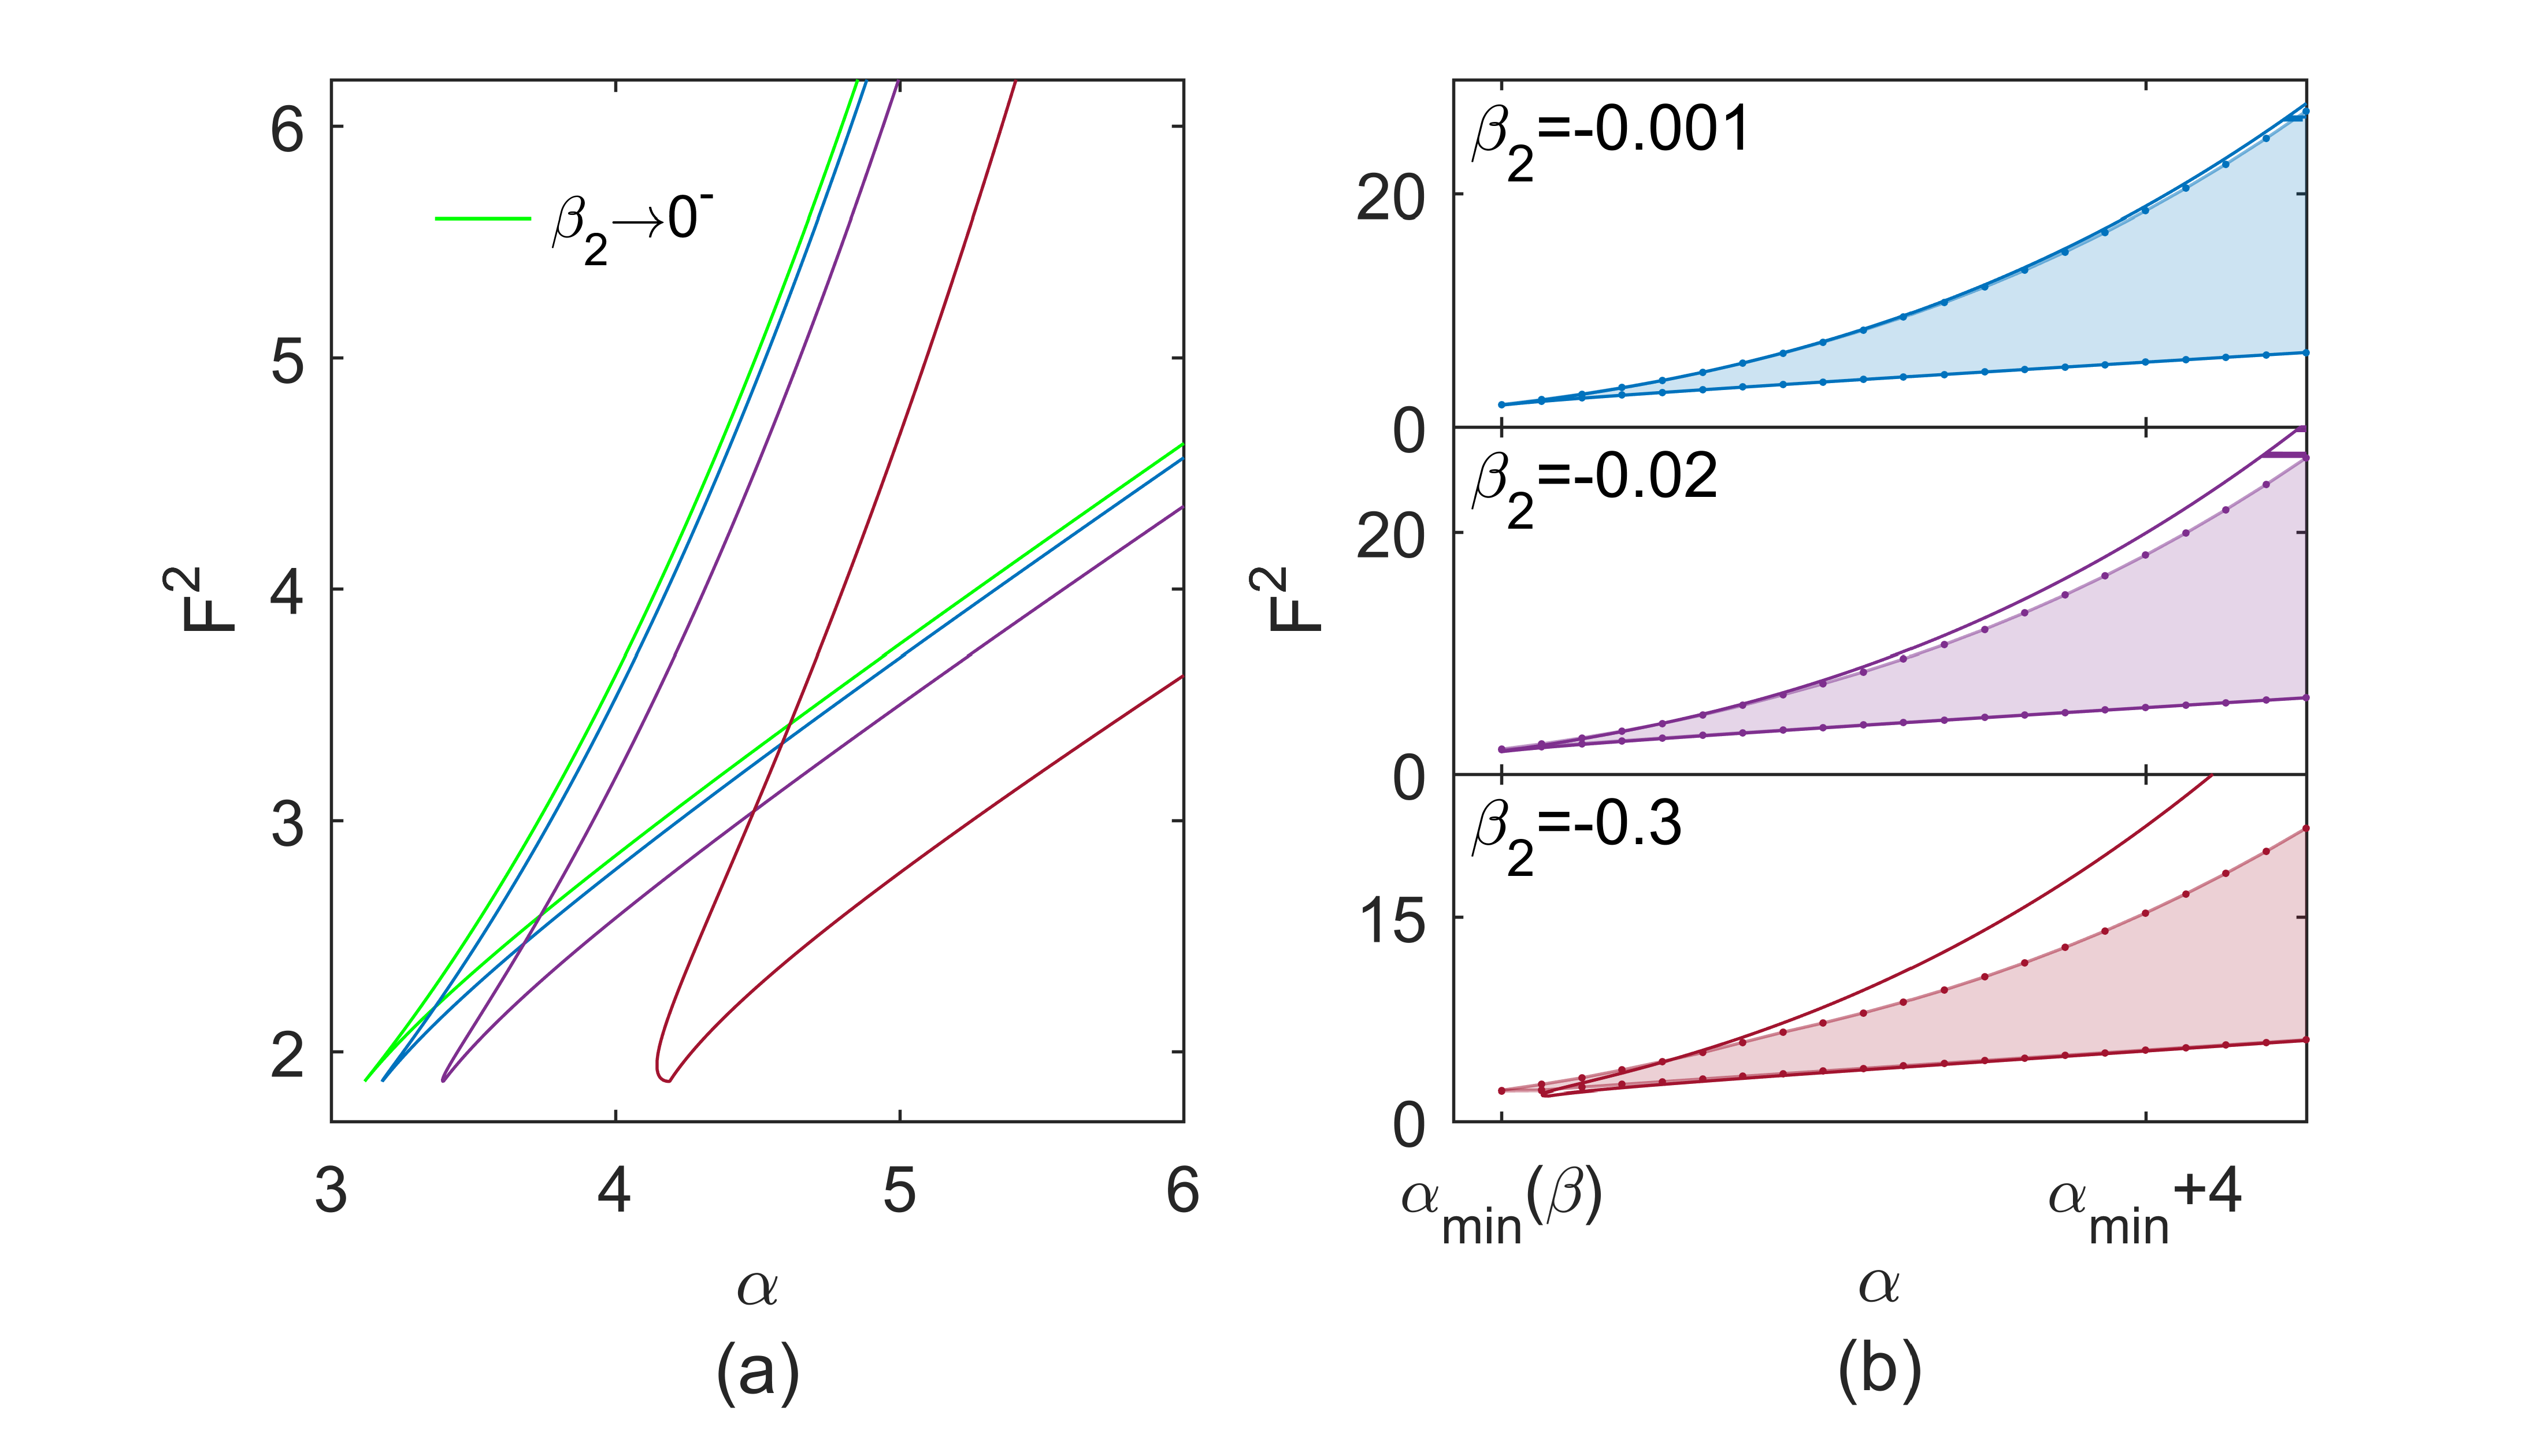
\includegraphics[]{\FigPath/Figures/FPLLE/FPLLEsolexistencerange.png}
	\end{center}
	\caption[Boundaries of soliton existence in the FP-LLE]{\textbf{Boundaries of soliton existence in the FP-LLE.} (a) Exact boundary of soliton existence for the limit $\beta_2\rightarrow0^-$ and analytical approximations to the boundaries for three finite values of dispersion: $\beta_2=-0.001$ (blue), $\beta_2=-0.02$ (purple), and $\beta_2=-.03$ (red). (b) Comparison between the finite-dispersion approximations from (a) and soliton existence boundaries as revealed by full simulations of the FP-LLE.  }
	\label{fig:FPLLEsolrange}
\end{figure} 

The lines $\alpha_{min} (F^2)$ and $\alpha_{max} (F^2)$ intersect at $F^2=F_I^2\approx1.87$. Below this value of the pump power solitons do not exist for the FP-LLE, and this can be seen as follows: The value of $\rho_{min}^\prime$ describing the amplitude of the soliton background along the line of maximum detuning $\alpha_{max}^\prime$ for the ring LLE is in general also a flat solution $\rho$ of the FP-LLE at the corresponding point $\alpha_{max}=\alpha_{max}^\prime+2\rho_{min}^\prime (\alpha_{max}^\prime,F^2)$. However, when $F^2<F_I^2\approx1.87$, the flat solution $\rho_{min}^\prime$ to the ring LLE is not the smallest flat solution to the FP-LLE; instead, it is the middle of three, and is therefore unstable. Therefore, when $F^2<F_I^2$ the line $\alpha_{max} (F^2)$ as defined above does not represent the right boundary of soliton existence for the FP-LLE. In fact, below this point, for all values of $\alpha$ where a stable flat solution to the FP-LLE $\rho_{min}$   exists, $\alpha-2\rho_{min} (\alpha,F^2 )>\alpha_{max}^\prime$, preventing the existence of solitons. This is an interesting contrast with the ring LLE, where the corresponding lines bounding soliton existence intersect at $F^2=1.175$ and where we can verify in simulations that solitons exist for e.g. $F^2=1.5$.


\section{Generation of single solitons through laser frequency scans}

A second important consequence of the additional nonlinear term in the FP-LLE relative to the ring LLE is an increase in the range of $\alpha$ values, for a given value of $F^2$, at which the state of $\psi$ can be either an extended pattern (spatiotemporal chaos or Turing pattern) or a soliton/soliton ensemble. This is because the extended patterns fill the domain and, because of their higher average intensity, experience a greater nonlinear shift than lower duty-cycle single solitons or soliton ensembles due to the additional nonlinear term. Here we discuss the implications of this fact for the experimental generation of single solitons through decreasing-frequency scans of the pump laser, as discussed in Chapter \ref{chap:microresonators}, Sec. \ref{sec:LLEsolitons}. We summarize the results in Fig. \ref{fig:FPLLE_C2S}.  In Fig. \ref{fig:FPLLE_C2S}a we show example simulations of spatiotemporal chaos and a single soliton to illustrate this degeneracy. Both of these simulations are conducted at the point $(\alpha=8,F^2=8)$, and the soliton and chaos are also degenerate with a stable flat solution, with the nature of $\psi$ dependent upon the initial conditions. 

\begin{figure}[htpb]
	\begin{center}
		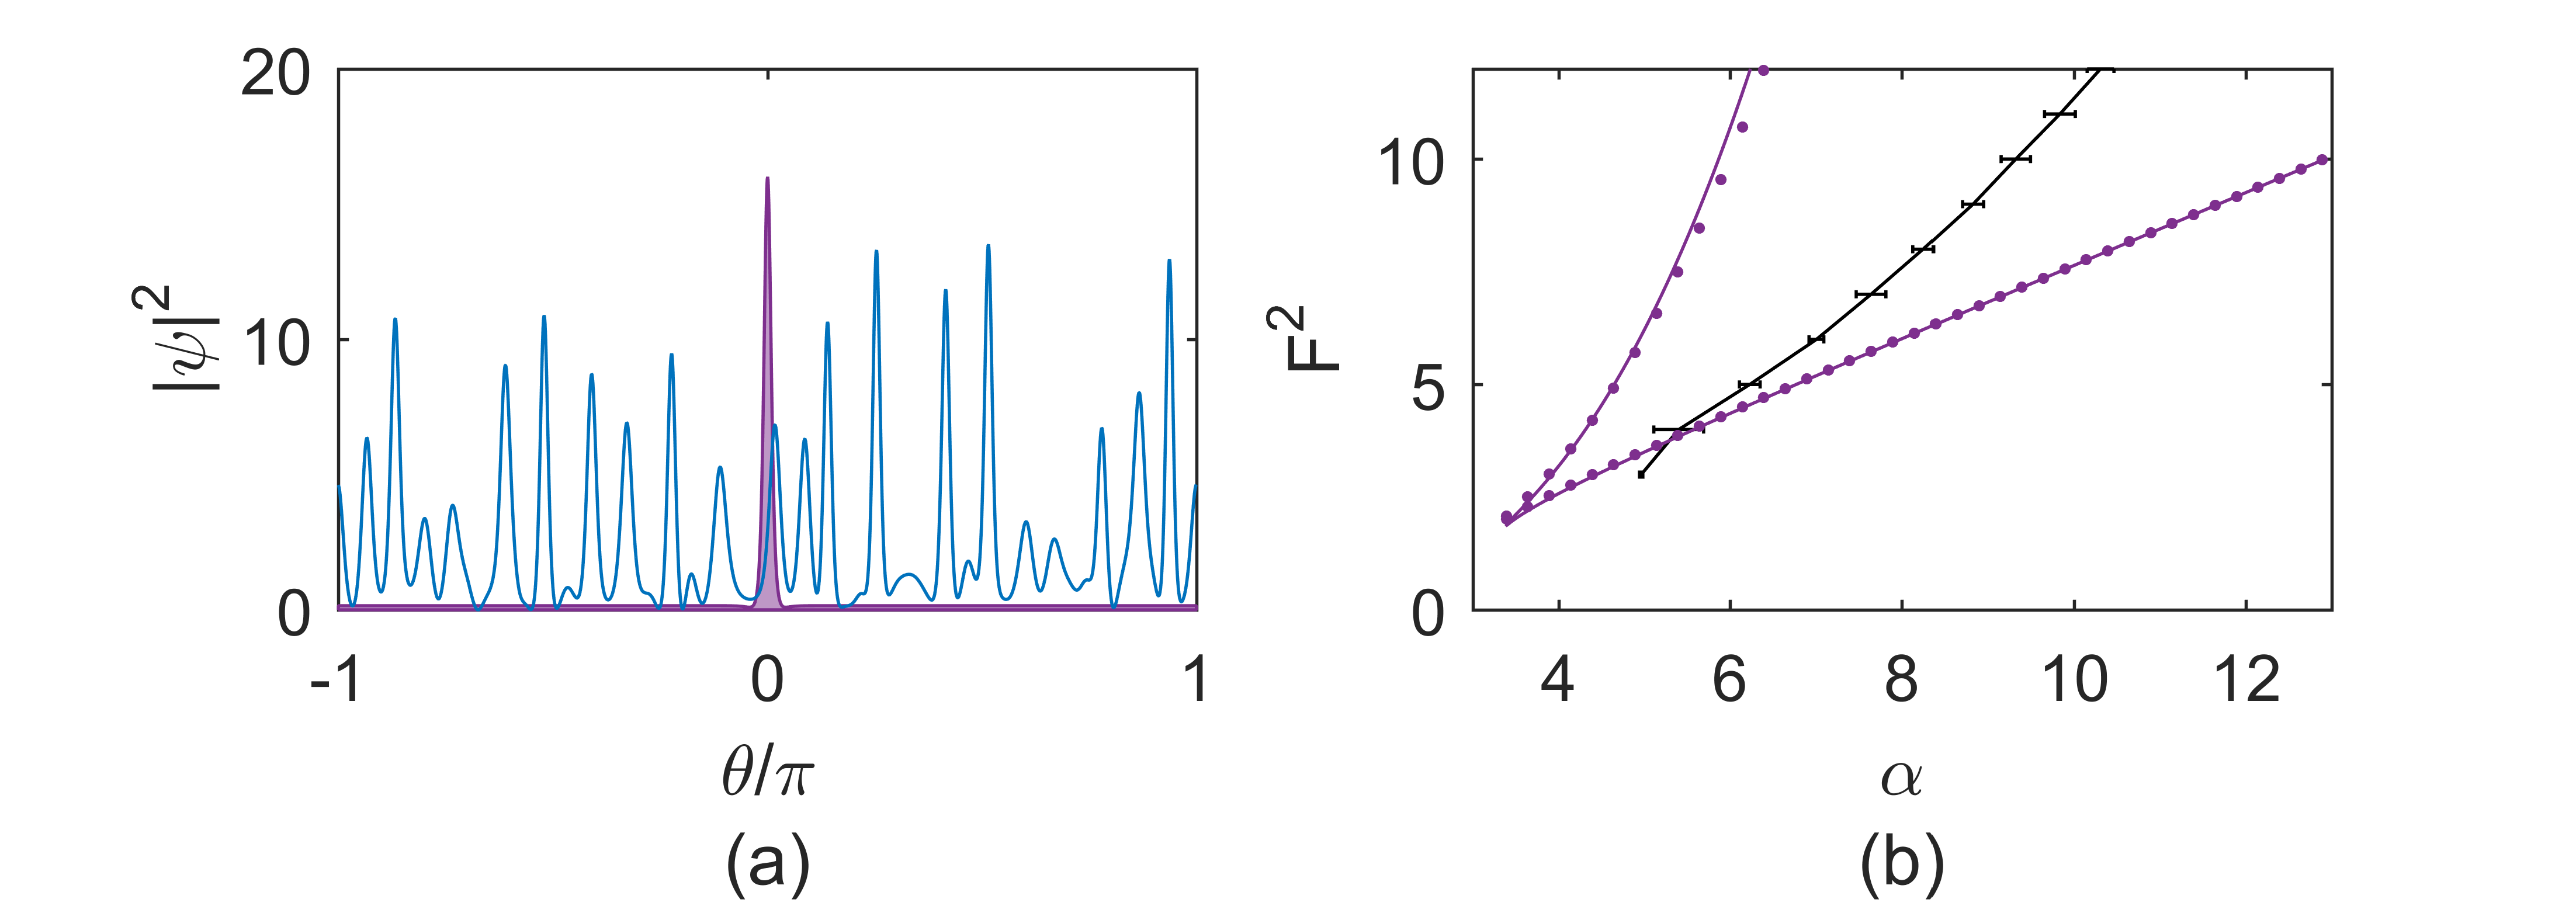
\includegraphics[]{\FigPath/Figures/FPLLE/FPLLE_C2S.png}
	\end{center}
	\caption[Transition from extended patterns to single solitons in the FP-LLE]{\textbf{Transition from extended patterns to single solitons in the FP-LLE.} (a) Simulated spatiotemporal chaos (blue) and single soliton solution (purple), either of which can exist at the point $(\alpha=8,F^2=8)$. The amplitude of the soliton is larger than the characteristic amplitude of the features in the chaos because the effective detuning $\alpha^\prime$ is larger for the soliton. (b) Analytical and numerical soliton existence limits (purple) for $\beta=-0.02$ from panel (a) and the upper bound in $\alpha$ for the existence of spatiotemporal chaos/Turing patterns (black with error bars), estimated as described in the text. }
	\label{fig:FPLLE_C2S}
\end{figure} 

It has been established that condensation of solitons from an extended pattern in a sweep in which $\alpha$ increases is a useful way of obtaining single solitons in experiments. Because this method relies on the excitation of an extended pattern (chaos or Turing pattern) to provide initial conditions out of which solitons condense as $\alpha$ is increased, it is important that the maximum detuning (the value of $\alpha$ where $\alpha^\prime=\alpha_{max}^\prime=\pi^2 F^2/8)$ for single solitons is larger than the $\alpha$ value at which an extended pattern will transition to a soliton ensemble. Otherwise, the generation of single solitons using this method will be difficult or impossible. To investigate this, we numerically perform slow scans across the resonance to identify where the transition from extended patterns to independent solitons occurs. These scans are conducted slowly to approximate adiabaticity: $d\alpha/d\tau=2.5\times10^{-4}$. We perform $10$ scans across the resonance at each integer value of $F^2$ from $3$ to $12$ with $\beta=-0.02$, and we identify the transition from extended pattern to independent solitons by inspection of several quantities as $\alpha$ is varied: the set of local maxima and minima of $|\psi|^2$ (see \cite{Coillet2014}), the distance between local maxima, and the number of local maxima above $|\psi|^2=1$. In Fig. \ref{fig:FPLLE_C2S}b we plot the line representing the upper boundary in $\alpha$ of extended patterns obtained in the scans across the resonance. Error bars represent the standard deviation of the values $\alpha$ at which the transition is observed, with this spread in the values arising due to the chaotic fluctuations in the total intracavity power and therefore also in the size of the nonlinear integral term. These results indicate that the region over which single solitons exist and extended patterns do not is narrow for small pump powers $F^2$, and widens as $F^2$ is increased. Without performing experiments, it is impossible to precisely quantify the limitations imposed by this observation, but we expect this finding to be useful in refining schemes for single-soliton generation in Fabry-Perot resonators. It is important to note that challenges associated with the necessary transition from high duty-cycle extended patterns to low duty-cycle solitons are alleviated by pulsed pumping, which was the technique used by Obrzud, Lecomte, and Herr in their recent report of soliton generation in FP resonators.




%
%
%shown by the upper blue line in Fig. \ref{Fig2}b. Explicitly (see Eqs. (\ref{statF2}) and (\ref{derF2zero}) and the accompanying discussion), this curve in the $\alpha-F^2$ plane is given by
%\begin{align}
%F_+^2(\alpha)&=F^2\left(\rho_-(\alpha),\alpha\right),\label{alphamin1}\\ 
%F^2(\rho,\alpha)&=\rho\left(1+(\alpha-3\rho)^2\right),\label{alphamin2}\\
%\rho_-(\alpha)&=\left(2\alpha-\sqrt{\alpha^2-3}\right)/9, \label{alphamin3}
%\end{align}
%so that the minimum detuning for solitons $\alpha_{min}(F^2)$ in the limit $\beta\rightarrow0^-$ (leading to zero soliton energy) is determined by inverting Eqs. (\ref{alphamin1})-(\ref{alphamin3}) to solve for $\alpha$ as a function of $F^2$. In the same limit of zero soliton energy, the maximum value of detuning for the FP-LLE at fixed $F^2$ is approximately $\alpha_{max}(F^2)=\alpha_{max}^\prime+2\rho_{min}^\prime\left(\alpha_{max}^\prime(F^2),F^2\right)$, where $\rho_{min}^\prime(\alpha^\prime,F^2)$ is the smallest solution to $F^2=\rho^\prime\left[1+(\alpha^\prime-\rho^\prime)^2\right]$ (here, as before, primed values are solutions of the appropriate equations for the ring LLE). These boundaries are plotted in Fig.~\ref{Fig7}a.
%
%For finite dispersion and soliton energy, numerical simulations show that the curves bounding the region of soliton existence are shifted as the energy of the soliton changes with dispersion. An intuitive way to understand the shift of the left boundary $\alpha_{min}$ is to note that the introduction of a soliton with finite energy onto a stable flat solution near and just right of the boundary $\alpha_{min}$ leads to a decrease in the effective detuning $\alpha_{eff}$ under which the flat solution evolves (due to the nonlinear integral term), and if this decrease is large enough it can lead to instability.
%
%A preliminary approximation to the dispersion-dependent boundary curves can be obtained using the analytical approximation to the soliton solution given by Eqs. (\ref{FPpsisolCW}-\ref{phioprime}). For fixed $\beta$ and $F^2$, we calculate the values of $\alpha$ at which the background $\rho^\prime$ of the soliton (given by Eq. (\ref{rhoprime})) is the same as the background along the zero-dispersion boundary curves; that is, for the dispersion-shifted left boundary we use the requirement $\rho^\prime=\rho_-$, and for the dispersion-shifted right boundary we use the requirement $\rho^\prime=\rho_{min}^\prime (\alpha_{max}^\prime (F^2),F^2)$. We compare the resulting curves with a numerical determination of the boundary curves for three finite values of dispersion; the results are plotted in Figs. \ref{Fig7}a and b. The analytical approximation is accurate for low $F^2$ and small dispersion, but becomes less accurate as these quantities increase. This is because breather solitons are found near $\alpha_{min}$ for larger values of $F^2$. Breather solitons are accompanied by traveling waves that propagate away from the soliton and diminish in amplitude as they do so, and their range increases with the dispersion. For larger values of dispersion these waves fill the cavity, and in this case the flat background whose stability forms the basis for approximating the dispersion-dependent boundary curves is actually not present. 
%
%The lines $\alpha_{min} (F^2)$ and $\alpha_{max} (F^2)$ intersect at $F^2=F_I^2\approx1.87$. Below this value of the pump power solitons do not exist for the FP-LLE, and this can be seen as follows: The value of $\rho_{min}^\prime$ describing the amplitude of the soliton background along the line of maximum detuning $\alpha_{max}^\prime$ for the ring LLE is in general also a flat solution $\rho$ of the FP-LLE at the corresponding point $\alpha_{max}=\alpha_{max}^\prime+2\rho_{min}^\prime (\alpha_{max}^\prime,F^2)$; this is due to the general correspondence between stationary patterns discussed in Sec. \ref{sec4}c. However, when $F^2<F_I^2\approx1.87$, the flat solution $\rho_{min}^\prime$ to the ring LLE is not the smallest flat solution to the FP-LLE; instead, it is the middle of three, and is therefore unstable. Therefore, when $F^2<F_I^2$ the line $\alpha_{max} (F^2)$ as defined above does not represent the right boundary of soliton existence for the FP-LLE. In fact, below this point, for all values of $\alpha$ where a stable flat solution to the FP-LLE $\rho_{min}$   exists, $\alpha-2\rho_{min} (\alpha,F^2 )>\alpha_{max}^\prime$, preventing the existence of solitons.
%
%

%
%For completeness, we note that after the transition to solitons, we observe in a small number of scans the onset of harmonic modelocking, by which we mean a slow (i.e. over hundreds or thousands of photon lifetimes) convergence of the soliton ensemble to uniform spacing. Because harmonic modelocking eliminates soliton collisions, which are the mechanism by which single solitons can be obtained from a multi-soliton ensemble, it is unclear whether single solitons can be generated under these conditions. Harmonic modelocking is clearly observed for all the scans for $F^2=3$, four of the scans for $F^2=7$, and one scan for $F^2=9$. While we have not investigated the phenomenon in depth, we speculate that harmonic modelocking occurs when a soliton ensemble exhibits a suitable initial distribution and an appropriate density of solitons, which is related to the pulse width and therefore to $\alpha$ and $\beta$.
%
%

% \chapter{Microresonator-based frequency combs: Summary and outlook}\label{chap:conclusion}

Chapters \ref{chap:microresonators}-\ref{chap:FPLLE} discussed generation of frequency combs from a continuous-wave laser by parametric frequecy conversion in Kerr-nonlinear resonators. I described three results: 1. The investigation and implementation of a technique for spontaneous soliton generation in Kerr resonators using a phase-modulated pump laser, 2. The observation and explanation of soliton crystals in Kerr resonators, and 3. A theoretical investigation of Kerr-comb generation in Fabry-Perot cavities, with an emphasis on the properties of solitons and soliton generation. These results all help to more clearly define what is possible with these systems, and suggest avenues for further research. 

Soliton generation with a phase-modulated pump laser is a promising candidate for inclusion in chip-integrated Kerr-comb systems as the mechanism by which single-soliton operation is initiated. Two directions for continued work are additional theoretical investigations of the full LLE with a phase-modulated pump, which could provide insight into the dynamics beyond what is possible using the approximations described in Chapter \ref{chap:PMpumping}; and implementation of the technique with resonators that have electronically-inaccessible free-spectral ranges, using the subharmonic-modulation approach that was proposed. Incorporation of the technique into a chip-integrated Kerr-soliton comb may also require modification and further devleopment of the technique that was used to overcome thermal instabilities associated with the increasing-frequency pump-laser scan.

The investigation of soliton crystals presented here serves several important purposes. First, it represented an important step towards full explanation of observed Kerr-comb phenomena in terms of the LLE model. \todo{am I citing pascal in sc chapter?} Second, soliton crystals have the attractive properties of single-soliton Kerr combs, with the additional property that a soliton crystal of $N$ pulses has conversion efficiency of pump-laser power into the comb that is roughly $N$ times higher than a comparable single-soliton comb. With careful preparation of a particular crystal state, this could make them attractive for applications like optical arbitrary waveform generation and nonlinear spectroscopy. Additionally, soliton crystals present a hugely degenerate configuration space that could be useful in implementations, for example, of an on-chip optical buffer or in communications applications \cite{Leo2010a}. Finally, experimental generation of soliton crystals is significantly simpler than generation of single solitons, where the change in the duty cycle of the optical waveform from extended pattern to single soliton leads to thermal instabilities that are alleviated only with precise control of the pump-laser power and frequency. Thus, it is possible to propose a scheme for deterministic on-chip soliton crystal generation that makes use of two resonators, each constructed of looped single-mode optical waveguides. One resonator is pumped by a laser and hosts the soliton crystal. The second resonator need not be pumped, and exists to provide a specific perturbation to the mode structure of the first resonator to enable soliton crystallization; this could be achieved through careful engineering of the coupling between the resonators. If the free-spectral range of the second resonator is considerably higher than the free-spectral range of the first, and not near one of its harmonics, then realization of single-mode perturbation to the mode structure of the first resonator could be achieved. Implementing deterministic soliton crystal generation on a chip in this way could greatly simplify requirements on the other components in a system for full-integration of Kerr solitons, as soliton generation could be achieved through slow tuning of the pump laser.

The theoretical investigation of Kerr-comb generation in the Fabry-Perot geometry will provide useful guidance for future experimental work. An obvious direction for continued work is the generation of solitons in Fabry-Perot cavities that make use of the additional degree of freedom provided by the dispersion applied by reflection at the ends of the cavity. This would build on previous experiments \cite{Braje2009,Obrzud2017}. In fact, soliton generation in Fabry-Perot cavities constructed of potted fiber ferrules with high-reflectivity end-coatings has already been realized at NIST Boulder \cite{Zhang2018}, but there remains work to be done to achieve control the total cavity dispersion with chirped mirror-coatings. Unresolved questions include the effect of uncontrolled expansion of the mode in the coating on both the mirror reflectivity and its group-velocity disperson. Looking to the chip scale, integrated Fabry-Perot cavities constructued of single-mode waveguides with photonic-crystal mirrors is a promising route for development that would further reduce the footprint of Kerr-comb systems. This work is ongoing at NIST Boulder, and primary comb has been observed in such a cavity \cite{Yu2018}. Finally, I note that the proposal for deterministic chip-scale generation of soliton crystals presented above could be realized with two co-linear on-chip Fabry-Perot cavities, where the first cavity hosts the crystal, which is out-coupled in reflection, and the second cavity provides a perturbation to the first cavity's mode structure.







  %read 6-27
% \chapter{EOM Combs}

In this chapter, I discuss the generation of high-repetition-rate frequency combs through electro-optic modulation of a continuous-wave laser – so-called EOM combs \cite{Kobayashi1972,Kourogi1993,Murata2000,Sakamoto2007,Morohashi2008,Ishizawa2010,Wu2010,Supradeepa2012,Metcalf2013,Wu2013}. This scheme represents an alternative to parametric generation of HRR combs in Kerr resonators, and as the technology matures it will likely find a niche in the application space that leverages its long-term stability, lack of moving parts, and possibility for robust turn-key operation. First I present the operational principle, and then experimental results that represent the first generation of a coherent octave-spanning supercontinuum and detection of an active-modulation-based frequency comb's carrier-envelope offset frequency without an external optical reference. Then I provide a detailed discussion of the noise properties of the EOM comb, the investigation of which is a significant contribution of the work described here. Finally, I provide a discussion of some possible future directions for the technology.

\section{Principle of operation}
Generally, the EOM comb concept consists of passing a CW 'seed' laser through cascaded phase and intensity modulators to generate a train of chirped pulses, and then propagating this pulse train through a dispersive medium to temporally compress the pulses to near their bandwidth-limited pulse duration. An generic expression for the electric field before temporal compression results from the product of the field $E_oe^{-i\omega_ct}$ with operators
\begin{align} \frac{1}{2}\left\{\mathrm{exp}\left[i(\phi_{DC}+\phi_{RF}\sin{\omega_rt})\right]+\mathrm{exp}\left[-i(\phi_{DC}+\phi_{RF}\sin{\omega_rt})\right]\right\}\\
=\cos\left(\phi_{DC}+\phi_{RF} \sin(\omega_rt+\phi_{IM-PM})\right)
\end{align} representing the intensity modulation and 
\begin{equation}
\mathrm{exp}\left[i\beta_m \sin{\omega_r t}\right]
\end{equation} representing the phase modulation. Here $E_o$ and $\omega_c$ are the complex amplitude and the carrier frequency of the seed laser. The phases  $\phi_{DC}$ and $\phi_{RF}$ represent the DC bias and depth of the intensity modulation, respectively, which experimentally are sourced from a DC power supply and an RF synthesizer. Writing the intensity-modulation operator as the sum of exponentials reveals the physical origin of intensity modulation as phase modulation in two paths with opposite sign. The phase-modulation index, which sets the initial bandwidth of the EOM comb, is $\beta_m$. The comb's repetition rate is $f_r=\omega_r/2\pi$, with $\omega_r$ the angular frequency of the phase and intensity modulation, which in practice are derived from the same synthesizer. The phase $\phi_{IM-PM}$ represents a phase difference between the IM and PM operators arising from path-length differences, which can be controlled via the insertion of a phase shifter in one electrical path. 

In practice, for subsequent spectral broadening of the comb it is desirable to configure the IM and PM to yield a train of 50 $\%$ duty-cycle pulses with normal chirp (temporally increasing carrier frequency). To achieve this, both $\phi_{DC}$ and $\phi_{RF}$ are set to $\pi/4$ and $\phi_{IM-PM}$ is set to zero. To achieve the former, the DC bias voltage and the RF modulation amplitude are adjusted to yield the appropriate optical spectrum for the seed laser with only intensity modulation applied. Setting $\phi_{IM-PM}$ to either zero or $\pi$ is achieved by examining the optical spectrum of the EOM comb with both IM and PM applied. The spectrum is asymmetric if $\phi_{IM-PM}$ is not zero or $\pi$ due to stronger transmission of either the high- or low-frequency components of the phase-modulated seed laser through the intensity modulators. The optical spectrum of the comb, which does not include phase information, is the same for $\phi_{IM-PM}=0$ or $\pi$; the difference between the two corresponds to reversal of the field in time or, equivalently, the difference between normal and anomalous chirp. In practice, setting $\phi_{IM-PM}$ to zero can be achieved by verifying that the pulses are compressed by propagation in an appropriate length of an anomalously dispersive medium; $\phi_{IM-PM}=\pi$ corresponds to anomalous chirp.

A simplified and illuminating expression for the electric field of a normally-chirped 50 $\%$ duty-cycle pulse train (up to a constant overall phase shift relative to the previous expression) is:
\begin{equation}
E=E_o\cos\left(\frac{\pi}{2}\sin^2{\frac{\omega_rt}{2}}\right)e^{i\omega_ct-i\beta_m\cos{\omega_rt}}.
\end{equation}
This can be understood as the product of a time-varying real amplitude $a(t)=E_o\cos\left(\frac{\pi}{2}\sin^2{\frac{\omega_rt}{2}}\right)$ and a phase factor from which the instantaneous carrier frequency $\omega(t)=\omega_c+\omega_r\beta_m\sin{\omega_rt}$ can be calculated. The carrier frequency $\omega(t)$ is increasing when the amplitude $a(t)$ is at its maximum, corresponding to normal chirp on the pulses.


\section{Detection of the carrier-envelope offset frequency of an EOM comb}

Here I describe generation of an EOM comb with 10 GHz repetition rate and subsequent measurement of its carrier-envelope offset frequency. The experimental setup is depicted in Fig. 1a. The basic experimental scheme consists of the following steps: 1. Initial generation and temporal compression of the EOM comb pulse train; 2. Modest spectral broadening and temporal re-compression; 3. Noise reduction using a Fabry-Perot filter cavity; and 4. Octave-spanning supercontinuum generation and detection of the carrier-envelope offset frequency. The results described below represent the first time a frequency comb based on active modulation of a CW laser has been self-referenced. Key to the success of this approach is the implementation of nonlinear spectral broadening in two stages, which allows the second stage to be seeded with $\sim$130 fs pulses for coherent supercontinuum generation. The noise reduction stage is also critical for coherent spectral broadening, and the investigation of its effects is a significant contribution of this work. 

To generate the initial train of chirped pulses, a telecom-band continuous-wave laser is passed through cascaded phase and intensity modulators driven with a 10 GHz microwave signal. The intensity modulator is biased at the 50 \% transmission point and driven with an RF amplitude appropriate for generation of a 50 $\%$ duty-cycle pulse train, as described above.   The phase modulator is driven with modulation depth of $\sim31\pi/4\sim24.3$ rad. The relative phase between the modulators is set such that the phase applied by the phase modulator is at a minimum when the transmission of the intensity modulator is highest; this yields a train of normally-chirped (up-chirped) pulses. Simulated temporal intensity and instantaneous carrier-frequency profiles are shown in Fig. 1b, and a simulated optical spectrum is overlaid on an experimental measurement in Fig. 1c.


\begin{figure}[htpb]
	\begin{center}
		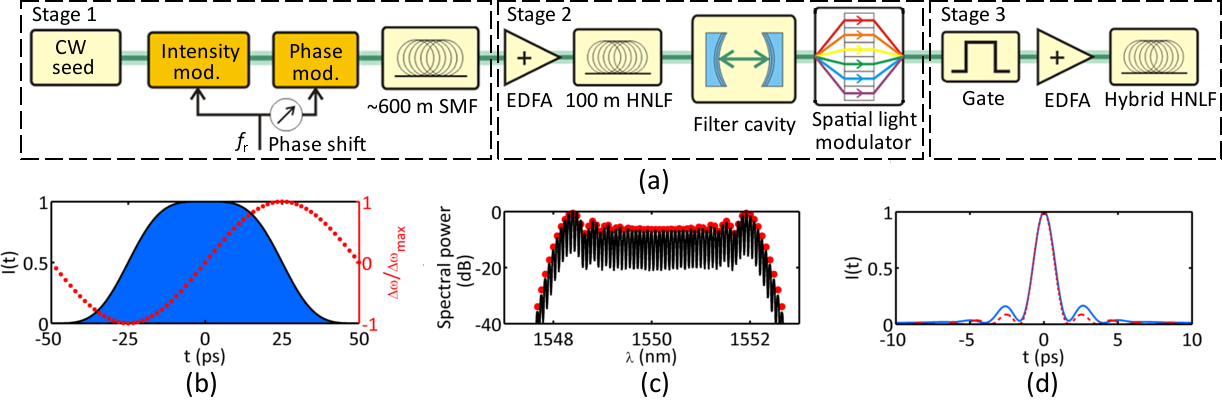
\includegraphics[width=15cm]{\FigPath/Figures/EOMCombs/EOMCSchematic.png}
	\end{center}
	\caption[Figure Title]{\textbf{Schematic and principle of operation for detection of the carrier-envelope offset frqeuency of an EOM comb.} (a) Experimental schematic for $f_0$ detection, with three stages: 1. Initial generation and temporal compression of the pulse train; 2. First stage of spectral broadening and temporal re-compression, along with noise suppression, and 3. Final stage of spectral broadening for generation of a coherent octave-spanning supercontinuum, including the implementation of an electro-optic gate for repetition-rate downsampling. (b) Depiction of a constituent pulse from a train of 50 $\%$ duty-cycle normally-chirped pulses with 10 GHz repetition rate. Intensity is shown in blue, and instantaneous carrier frequency is shown in red. The periodic electric field of this pulse train is given by Eqn. \ref{Eqn:EOMC} (c) Measured optical spectrum of the initial EOM comb pulse train (black), along with the simulated spectrum corresponding to the plots in panel (b). (c) Simulated temporal compression of the pulses shown in panel (b), with compression conducted by propagation in 570 m of SMF (solid blue) and compression to the transform limit (dashed red). The full-width at half-maximum (FWHM) duration of both pulses is $\sim$1.5 ps.   }
	\label{fig:EOMC_Schematic}
\end{figure} 


Next, the chirped pulse train is propagated through 600 m of anomalously-dispersive SMF. The length of SMF that is appropriate for pulse compression depends on the bandwidth of the optical pulses to be compressed; equivalently, it depends on both the phase-modulation depth and the repetition rate of the pulse train. This temporal compression reduces the duration of the optical pulses from $\sim$50 ps to $\sim$ 1.5 ps. A simulation of the resulting intensity profile is presented in Fig. 1d. 

The compressed pulses are amplified to 400 mW average power in an erbium-doped fiber amplifier and launched into 100 m of HNLF. This section of HNLF has chromatic dispersion that is small and normal; this is carefully chosen to chirp the pulses via self-phase modulation while avoiding soliton-fission dynamics\cite{Dudley2006}. The result is a train of chirped $\sim$1.5 ps pulses exiting the fiber.  In Fig. 2a we present the measured optical spectrum of this pulse train, as well as results of a numerical simulation of the spectral broadening in the 100 m of normally-dispersive HNLF. These simulations are conducted using the nonlinear Schrodinger equation (NLSE) including third order dispersion\cite{Agrawal2007}, taking as initial conditions the calculated intensity profile of the EOM comb pulses shown in Fig. 1d. The dispersion values for the HNLF used in the simulation are $D=-0.04$  ps/nm$\cdot$km and $D'=0.003$ ps/nm$^2\cdot$km, close to the values specified by the manufacturer. The simulation method is described in detail in App. \ref{NumericalSims}.

After propagation through the first section of HNLF, the pulses are passed through a high-finesse Fabry-Perot cavity for suppression of optical frequency fluctuations as discussed below. Then the pulses are temporally compressed again, this time using a commercial spatial light modulator (SLM) \cite{Weiner2000}; the SLM separates narrow spectral regions using a grating and passes them through individually controlled delaying elements before recombination. The SLM applies 2\textsuperscript{nd}, 3\textsuperscript{rd}, and 4\textsuperscript{th} order chromatic dispersion, which simulations indicate is sufficient to compress the chirped pulses to $\sim$130 fs, near their transform limit. This is shown in Fig. 2b. While it is convenient, the SLM is not strictly necessary; it would also be possible to compress the pulses via propagation in an appropriate length of SMF. Figs. 2b and 2c present the output intensity profile and the evolution of the intensity profile, respectively, in simulated compression in SMF. Because the pulses are broadband, temporally short, and reasonably high energy, these simulations include the full dispersion profile of SMF and the Kerr nonlinearity.



The temporally compressed $\sim$130 fs pulses are then passed through a Mach-Zehnder modulator functioning as an electro-optic gate for repetition-rate downsampling (see Chapter \ref{PulsePicking}). The gate selectively transmits every fourth pulse, reducing the repetition rate of the pulse train to 2.5 GHz. This facilitates coherent supercontinuum generation in a second stage of spectral broadening by increasing the pulse energy that can be achieved at a given average power. Note that this step is convenient but not strictly necessary, as shown in Ref. \cite{Beha2017}. 

The downsampled 2.5 GHz pulse train is amplified to an average power of 1.4 W, resulting in a train of $\sim$0.56 nJ pulses. This pulse train is propagated through 8 m of hybrid HNLF, yielding the spectrum shown in Fig. 2d. This hybrid HNLF consists of two segments with different dispersion profiles, with each segment serving a different purpose. The first segment is 30 cm long and highly dispersive ($D=6$  ps/nm$\cdot$km), and generates a dispersive wave centered at 1090 nm. The second segment is 7.7 m long and has lower dispersion ($D=1.5$  ps/nm$\cdot$km), and generates a Raman-self-frequency-shifted soliton centered near 2150 nm. The effect of each of these fibers on the output spectrum can be understood by investigating propagation in each section separately. To do this we use the LaserFOAM program \cite{Amorim2009}, which employs the generalized NLSE including Raman scattering, self-steepening, and 2nd- through 4th-order dispersion. The simulations are run independently, and both take as their initial conditions 170 fs Gaussian pulses with 350 pJ energy, close to the energy coupled into the HNLF after accounting for losses. The results of these simulations are plotted in Fig. 2d. 

 % % % % % PulsePickedTrains]
\begin{figure}[htpb]
	\begin{center}
		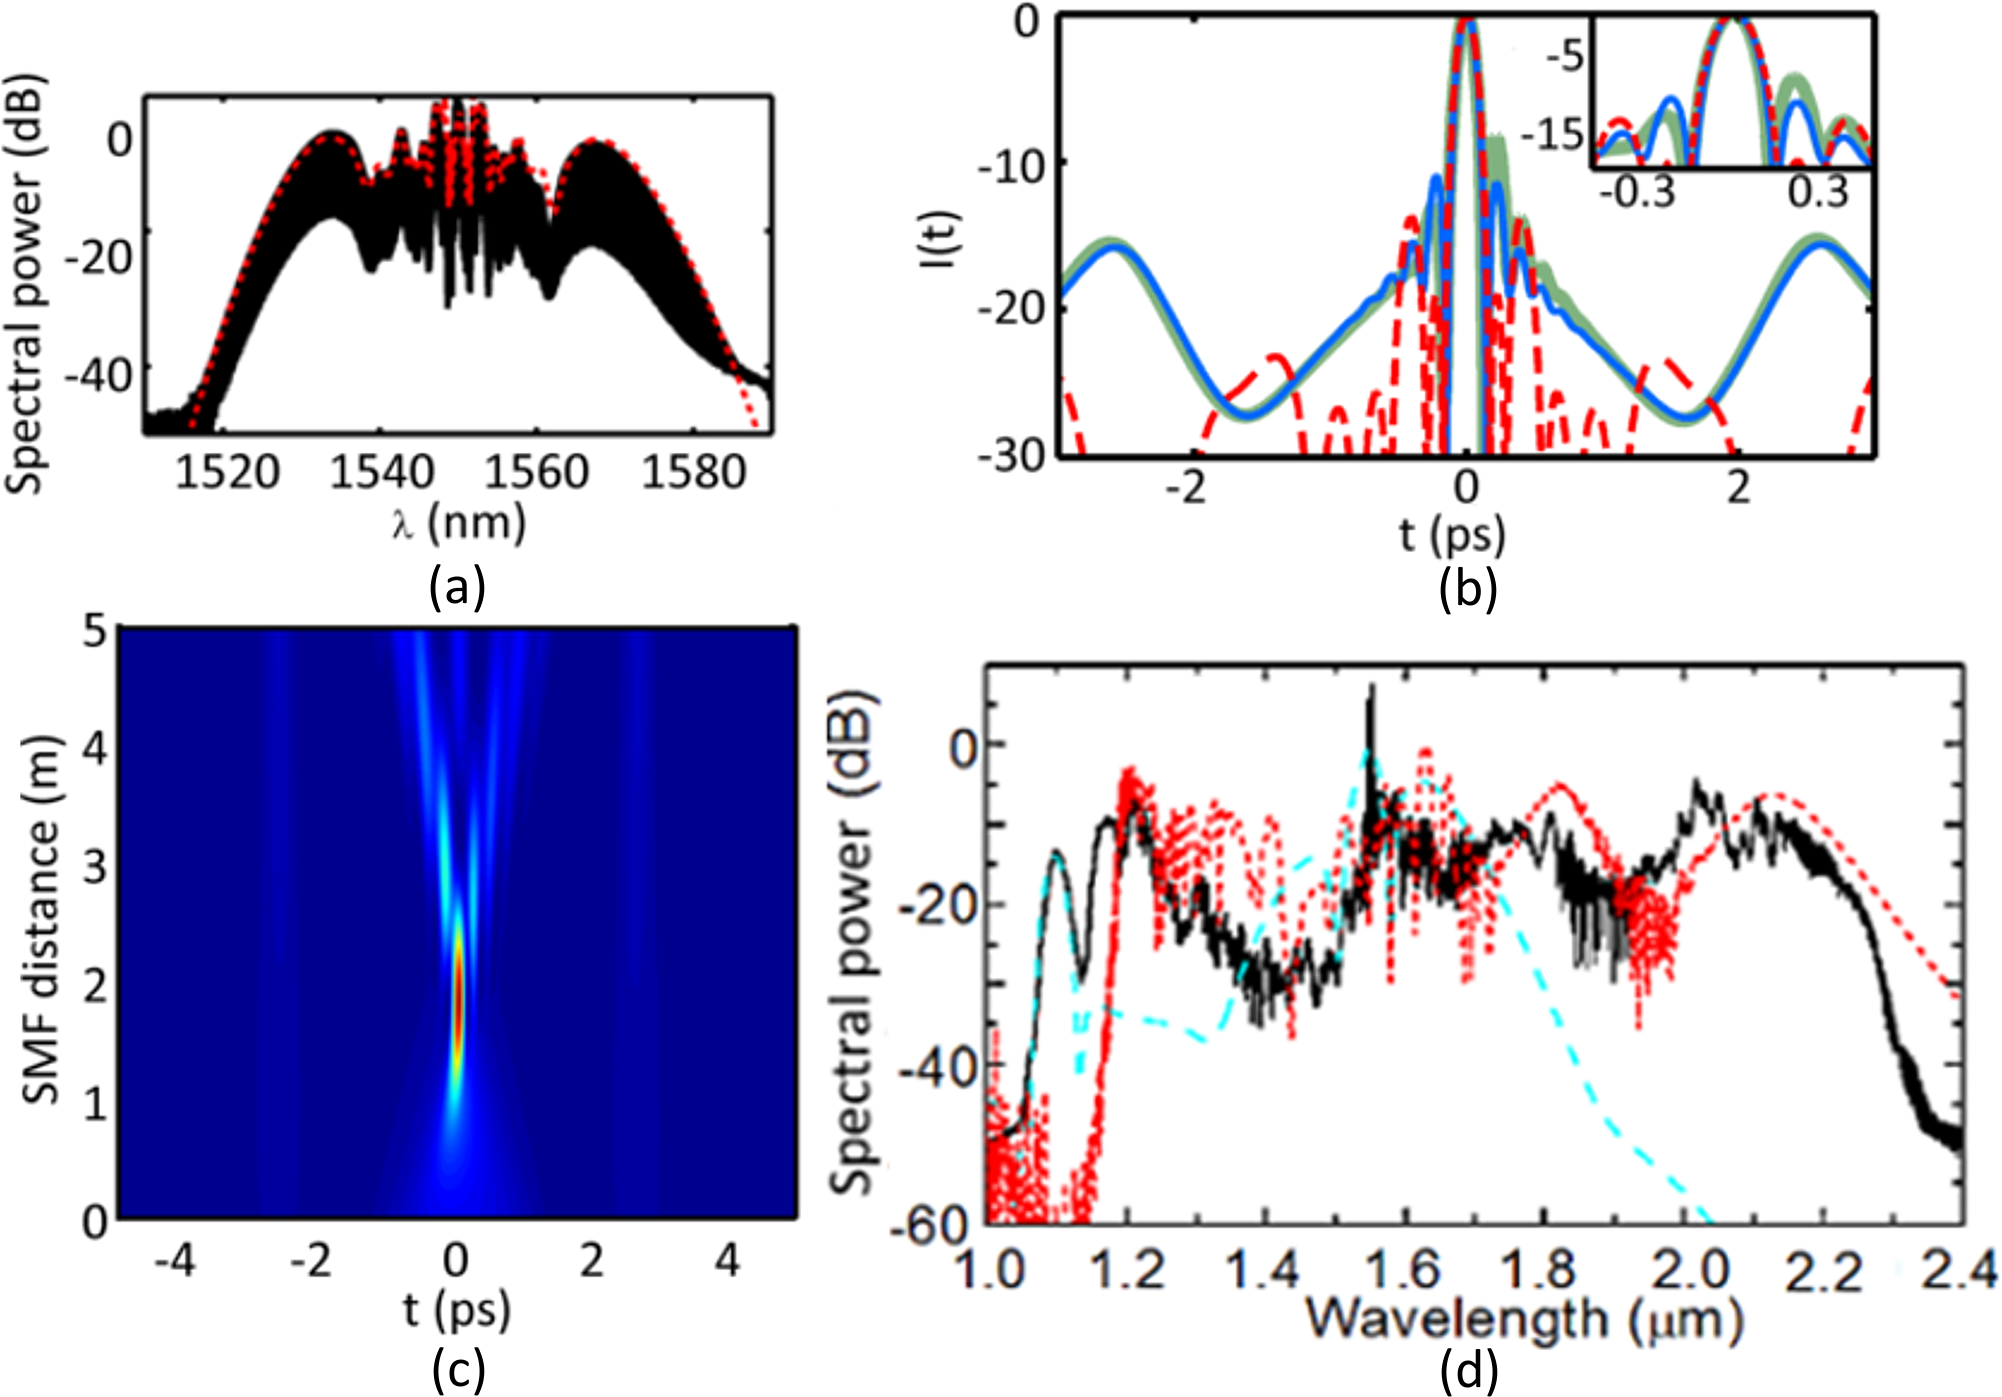
\includegraphics{\FigPath/Figures/EOMCombs/EOMC_spectraWsims.png}
	\end{center}
	\caption[Figure Title]{\textbf{Spectral broadening for generation of an octave-spanning supercontinuum.} (a) Measured optical spectrum after propagation in 100 m of low-normal-dispersion HNLF (black). The spectrum is broadened by self-phase modulation, which imposes a chirp on the pulses. Shown in red is a simulation of the same, conducted as described in the text. (b) Logarithmic-scale plot of the simulated pulse intensity envelopes after temporal recompression in the SLM with 2\textsuperscript{nd}-, 3\textsuperscript{rd}-, and 4\textsuperscript{th}-order dispersion (blue), in an appropriate length of SMF (thick green), to the transform limit (dashed red). (c) Simulated re-compression of the SPM-chirped pulses (red spectrum in panel (a)) in SMF. (d) Measured optical spectrum of the octave-spanning supercontinuum generated by the EOM comb system (black), plotted along with simulated spectra calculated as described in the text to investigate the effects of the 30 cm, highly-dispersive piece of HNLF (long-dashed teal) and the 7.7 m, lower-dispersion piece of HNLF (short-dashed red).}
	\label{fig:EOMC_Broadening}
\end{figure} 

The supercontinuum generated in the hybrid HNLF is coherent and suitable for $f-2f$ self-referencing (see App. \ref{App:f-2f}). To detect the carrier-envelope offset frequency of the EOM comb, we pass the pulse train through an interferometer consisting of a dichroic mirror, a delay stage in one path, and a 10 mm sample of periodically-poled lithium niobate that generates the second harmonic of supercontinuum light at 2140 nm.  The dichroic mirror and delay stage enable adjustment of the relative timing between the native 1070 nm and doubled 2140 nm components of the supercontinuum so that they are temporally coincident. An optical band-pass filter centered at 1070 nm selects the supercontinuum components required for self-referencing, shown in Fig. 3a, and impinging the filtered light on a photodetector reveals the carrier-envelope offset frequency of the EOM comb, shown in Fig. 3b. Note that downsampling introduces an ambiguity in the offset frequency due to the increased density of comb modes in the downsampled pulse train; this ambiguity can be removed by measuring the change in measured offset frequency with a change in $f_r=\omega_r/2\pi$ provided by the synthesizer driving the modulators. 




\begin{figure}[htpb]
	\begin{center}
		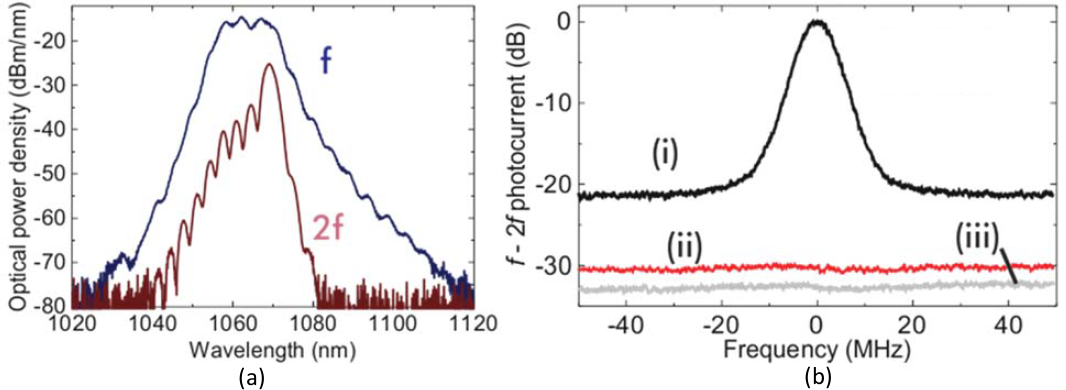
\includegraphics[width=15cm]{\FigPath/Figures/EOMCombs/EOMC_f0fromOptica.png}
	\end{center}
	\caption[Figure Title]{\textbf{Self-referencing of an EOM comb.} (a) Spectral components used for $f-2f$ self-referencing after passing through a 1070-nm optical bandpass filter: \color{red}native supercontinuum light (blue) and frequency-doubled 2140-nm supercontinuum light (red) ARE THESE LABELED CORRECTLY\color{black}. (b) Photodetected carrier-envelope offset frequency signal (black), along with a measurement of the intensity noise of the pulse train obtained by \color{red} blocking one of the paths (red) \color{black}and the photodetector noise floor (grey). \color{red}The intensity-noise measurement highlights the presence of a broad background noise floor  on the $f_0$ signal that must be the result of frequency fluctuations because it is not present when photodetecting either path alone.\color{black}}
	\label{fig:EOMC_f0}
\end{figure} 



\section{Noise in EOM Combs}

An important difference between the EOM comb scheme and other approaches for generation of frequency combs is that the repetition rate is derived from a microwave source and is multiplied directly by a factor $N$ to yield the optical frequency of the frequency-comb mode with number $N$ referenced to the seed laser (where $N=0$). Therefore, the contribution to the optical frequency noise of mode number $N$ from the microwave source scales with the mode number $N$, and the contribution to the power spectrum of frequency noise scales as $N^2$. This presents a challenge in the generation of coherent supercontinuum light, where the modes relevant for $f-2f$ self-referencing are far separated from the seed laser and $N$ is large. The factor by which the noise on the modulation tone $f_r$ is multiplied to determine its contribution to the noise on the measured carrier-envelope offset frequency is the ratio between the comb’s carrier frequency (the frequency of the seed laser) and the repetition rate: $N=f_c/f_r=$19340 for the 10 GHz comb discussed above (where $f_c=$193.4 THz for a 1550 nm seed laser). This contribution is shown in Fig. 3a, along with the contribution from the CW seed laser. The noise on $f_r$ results from technical noise on the synthesizer tone at low Fourier frequencies and approaches a white Johnson-Nyquist (thermal) phase-noise floor of -177 dBm/Hz at high Fourier frequencies. Noise in each of these regimes impacts the photodetected $f_0$ signal: low-frequency noise contributes to the linewidth of the comb modes and therefore the $f_0$ signal, while high-frequency noise contributes to a frequency-noise floor on the photodetected signal\cite{Domenico2010}. As discussed in Ref. \cite{Beha2017}, unmitigated multiplication of this noise floor by the factor $N^2=$19340$^2$ leads to a supercontinuum with optical frequency fluctuations that are large enough to prevent detection and measurement of $f_0$. 

To address this problem and enable $f-2f$ self-referencing of our comb, we pass the comb through a Fabry-Perot filter cavity whose free-spectral range is actively stabilized to the comb’s mode spacing. The filter cavity’s Lorentzian transfer function reduces the optical frequency fluctuations of the comb modes at high frequency – these fluctuations are averaged over the photon lifetime of the cavity. This enables generation of a supercontinuum with resolvable modes that is suitable for $f-2f$ self-referencing and measurement of $f_0$. 

The filter cavity used for this 10 GHz comb has a 7.5 MHz linewidth; equivalently, it has finesse of $F\sim$1333. The effect of passing the comb through the cavity is demonstrated concretely in Fig. 3b, where we compare the lineshape of a heterodyne beat between the supercontinuum and a CW laser with 1319 nm wavelength with and without the filter cavity in place. The signal-to-noise ratios for the beat with and without the filter cavity are 40 dB and 17 dB, respectively.


\begin{figure}[htpb]
	\begin{center}
		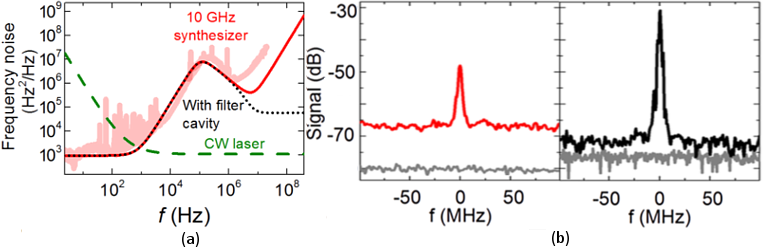
\includegraphics[width=15cm]{\FigPath/Figures/EOMCombs/EOMC_NoiseFigure_thesis.png}
	\end{center}
	\caption[Figure Title]{\textbf{Investigation of the noise properties of the EOM comb.}  (a) Contributions to the fluctuation spectrum of the carrier-envelope offset frequency: model of the input seed laser (dashed green), model of the 10 GHz synthesizer multipled by 19430$^2$ without the filter cavity (solid red, experimental data thick red), and synthesizer multiplied by 19340$^2$ and the Lorentzian filter-cavity transfer function (dotted black). (b) Comparison of the detected beats between the supercontinuum and a 1519 nm-wavelength CW laser without (red, left) and with (black, right) the Fabry-Perot filter cavity. The level of intensity noise on the supercontinuum, measured by removing the 1319 nm CW laser, is shown by the lower gray trace in each plot. Signal-to-noise ratios for the beat are 17 dB without and 40 dB with the filter cavity.}
	\label{fig:EOMC_noise}
\end{figure} 

We also explore the effect of low-frequency fluctuations in the modulation tone $f_r$ by changing the source of this tone. The $f_0$ signal shown in Fig. \ref{Fig:EOMC_f0}b is acquired with a tunable commercial synthesizer providing $f_r$. In Fig. \ref{Fig:EOMC_f0_sources} we show the detected $f_0$ signal with a dielectric-resonator oscillator and a sapphire oscillator providing $f_r$; these sources have less low-frequency noise, and the effect of this lower noise is readily apparent in the reduced linewidth of the $f_0$ signal.



\begin{figure}[htpb]
	\begin{center}
		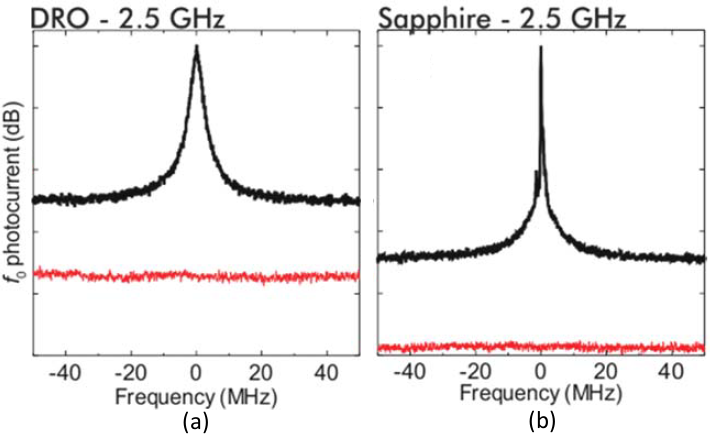
\includegraphics[width=10cm]{\FigPath/Figures/EOMCombs/EOMC_f0_diffosc_thesis.png}
	\end{center}
	\caption[Figure Title]{\textbf{Photodetected carrier-envelope-offset frequency signal with different sources for $f_r$.} (a) The $f_0$ beat resulting from a dieletric-resonator oscillator source for the modulation frequency. (b) Ibid with a sapphire oscillator as the source for $f_r$, which has lower noise than both the tunable commerical synthesizer and the DRO. The reduction in linewidth associated with the change in the source for $f_r$ shows the effect of low-Fourier-frequency noise of $f_r$ on the frequency-noise characteristics of the EOM comb. }
	\label{fig:EOMC_f0_sources}
\end{figure} 




% \chapter{Downsampling of optical pulse trains} \label{chap:PulsePicking}
    \begin{footnotesize}
 	\begin{spacing}{1.2}
 		This chapter describes work that was reported in:
 		\begin{itemize}
 			\item \fullcite{Cole2018b}.\\
 		\end{itemize}
 	\end{spacing}
 \end{footnotesize}
 

This chapter presents a discussion of a technique for repetition-rate reduction of optical pulse trains. While high pulse train repetition rates are appealing for some applications, they are not always appropriate. For example, spectral resolution in spectroscopy applications is sacrificed in a comb with a large mode spacing, and a high repetition rate makes nonlinear optics less efficient at a given average power. This can present a barrier to the generation of octave-spanning spectra for $f-2f$ self-referencing. On the other hand, in general the size of the comb package sets the scale for the round-trip time, meaning that low-SWAP combs tend to have inherently high repetition rates. Therefore, to increase the flexibility of low-SWAP and high repetition-rate comb systems in applications, a method for reducing the repetition rate of a pulse train will be useful.

We consider a method for pulse train repetition-rate reduction, or downsampling, in which an electro-optic gate realized by an RF-driven intensity modulator periodically transmits an incoming pulse at a frequency lower than the input repetition rate. The basic principle is illustrated in Fig. \ref{fig:PPConcept}. Downsampling via pulse gating, also referred to as `pulse picking' in the literature, has been used extensively in the context of high-field, phase-sensitive ultrafast optics for the generation of energetic, carrier-envelope-phase-stabilized ultrashort pulses \cite{Backus1998,Baltuska2003}. In this application, a comb with initial repetition rate in the $\sim$100 MHz range that has already been self-referenced and stabilized is pulse-picked to a repetition rate on the order of 1-100 kHz. Concerns in this application center around control and preservation of the carrier-envelope phase in the pulse-picking and amplification process \cite{Gohle2005,Rauschenberger2006}. In contrast, the focus here is on downsampling within the context of optical metrology with frequency combs, and we are concerned with downsampling's effect on the optical phase noise, the pulse-to-pulse energy fluctuations, and the carrier-envelope offset frequency of the comb. In particular, it is important that the downsampled pulse train is suitable for $f-2f$ self-referencing. 

Sec. \ref{sec:PPProofOfPrinciple} presents a proof-of-principle experiment in which a 250 MHz pulse train is downsampled to 25 MHz, and then spectrally broadened and self-referenced. A mathematical model of downsampling is presented in Sec. \ref{sec:PPMath}, and this model informs the discussion of downsampling's effect on the pulse train's noise properties presented in Sec. \ref{sec:PPNoiseExp} and Sec. \ref{sec:PPNoiseTheory}. In Sec. \ref{sec:PPAmplification} we discuss some practical considerations in applications of the technique, including the effect of imperfections in the gating process such as incomplete extinction of rejected pulses.



 % % % % % PulsePickedTrains]
\begin{figure}[htpb]
	\begin{center}
		%		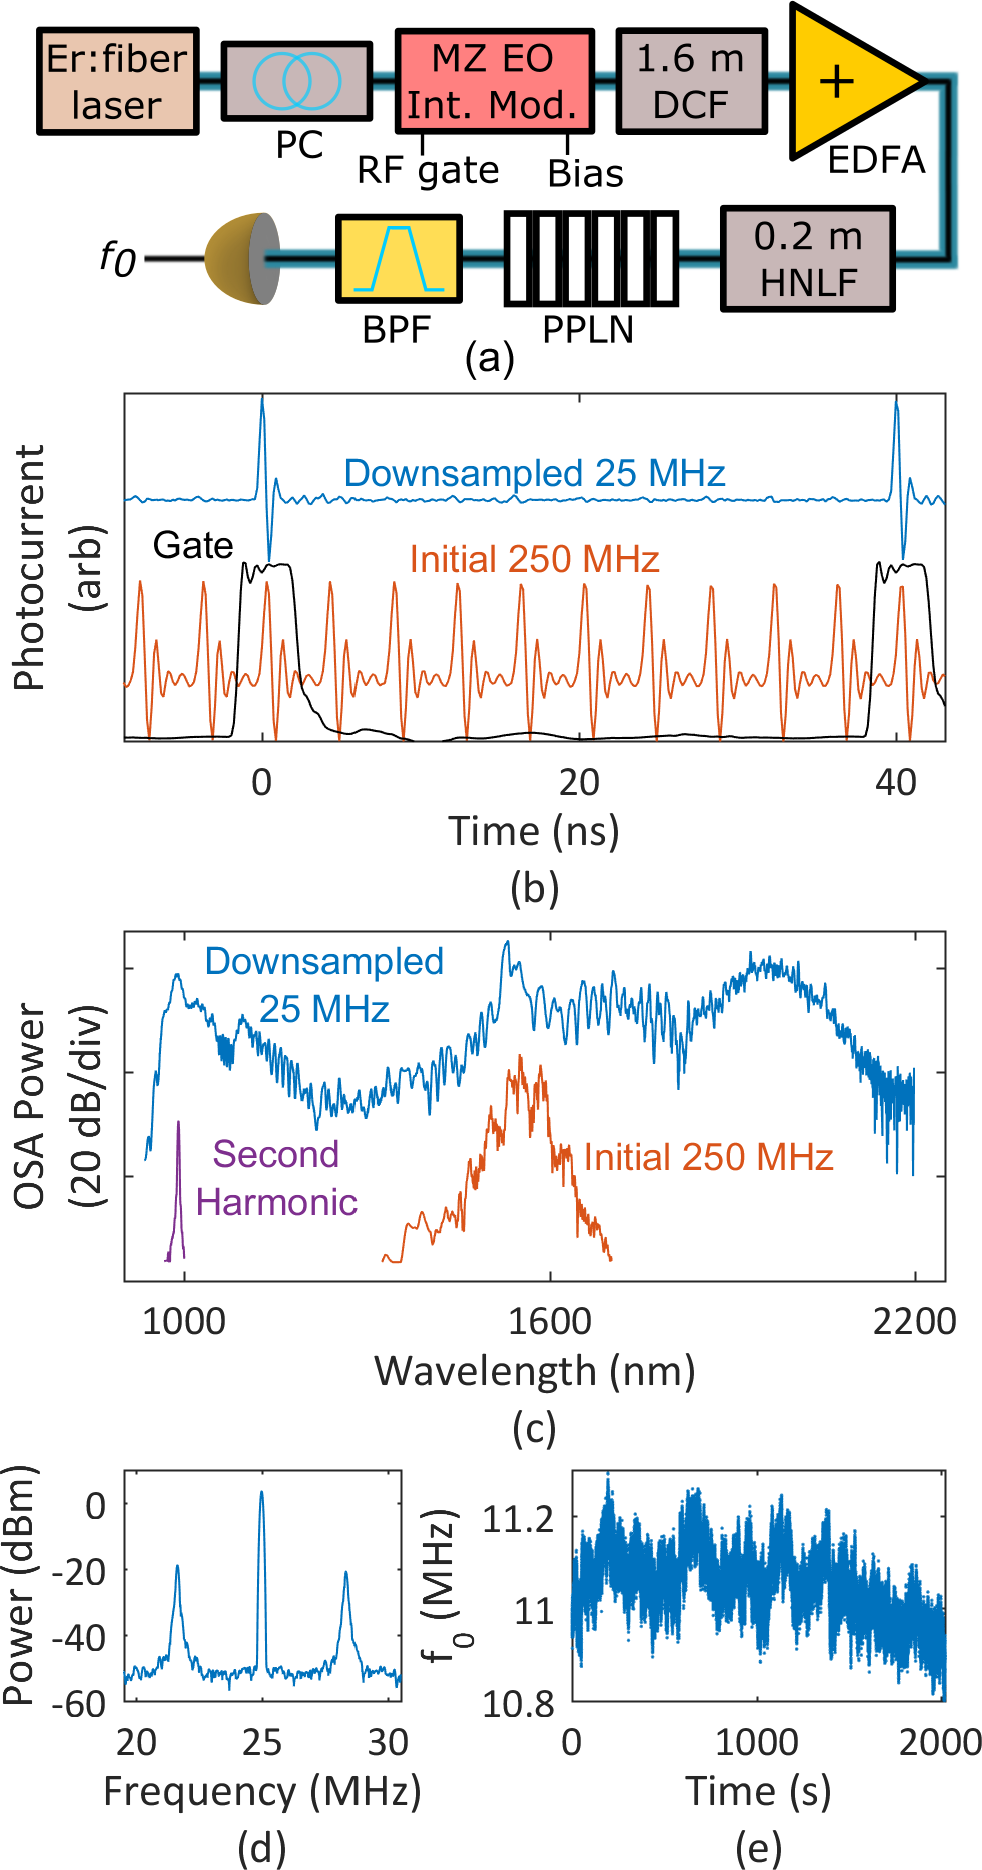
\includegraphics[width=110mm]{\FigPath/Figures/PulsePicking/PulsePickingPaperFig1.png}
		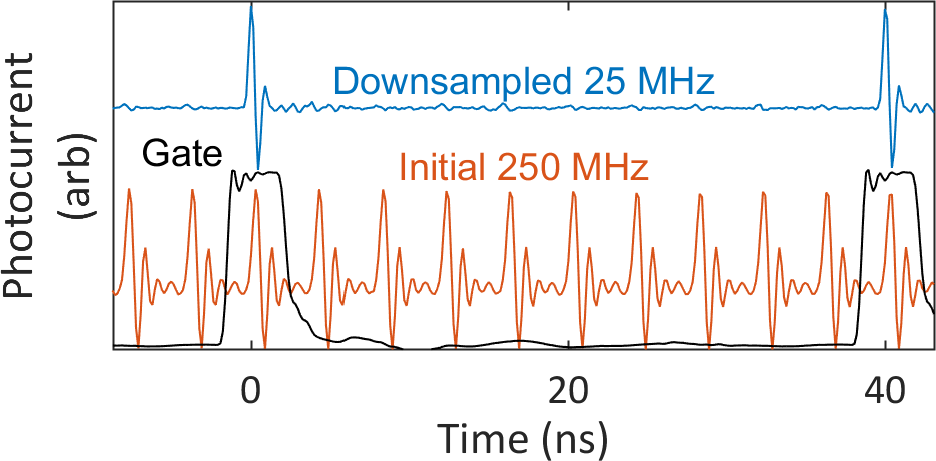
\includegraphics[width=110mm]{\FigPath/Figures/PulsePicking/PulsePickedTrains.png}
	\end{center}
	\caption[An illustration of pulse-train repetition-rate downsampling]{\textbf{An illustration of pulse-train repetition-rate downsampling.} Orange: A photodetected 250 MHz pulse train. Blue: A photodetected 25 MHz pulse train obtained by downsampling the 250 MHz pulse train by a factor of $N=10$. Black: Oscilloscope trace showing the voltage sent to the RF port of a Mach-Zehnder intensity modulator to selectively transmit a subset of the incoming pulses. With the intensity modulator biased for zero transmission, the voltage trace is indicative of the transmission.}
	\label{fig:PPConcept}
\end{figure} 





\section{Proof-of-Concept Experiment}\label{sec:PPProofOfPrinciple}
Here we present a proof-of-concept experiment in which a 250 MHz comb is downsampled and self-referenced. The setup for and results of this experiment are summarized in Fig. \ref{fig:PPDemo}. Our pulse gating scheme, shown in Fig. \ref{fig:PPDemo}a, employs a Mach-Zehnder (MZ) electro-optic intensity modulator driven by 25 MHz rectangular electronic gating pulses with 80 ps transitions and 3.5 ns duration. The electronic pulse generator and the repetition rate of the input 250 MHz comb are both referenced to a hydrogen maser to maintain synchronization. The DC bias of the intensity modulator is set for maximum extinction outside the electronic gate, whose amplitude is approximately matched to $V_\pi$ of the EOM. This downsampling scheme results in a stable 25 MHz optical pulse train with $>$12 dB contrast (Fig. \ref{fig:PPConcept}). This contrast is adequate for this experiment, but could be improved by cascading modulators with higher extinction ratios.  The average power of the 250 MHz pulse train is reduced from 30 mW to 400 $\mathrm{\mu}$W by the pulse gating process and the insertion loss of the optical components. The pulse train is amplified to 35 mW by use of a normal-dispersion erbium-doped fiber amplifier, which provides some spectral broadening and temporal pulse compression \cite{Fermann2000}. An octave-spanning supercontinuum is obtained by launching the amplified, $<$100 fs, $\sim$1 nJ pulses into 20 cm of highly nonlinear fiber (HNLF) \cite{Hirano2009}; the resulting spectrum is shown in Fig. \ref{fig:PPDemo}b.  For comparison, we also present the supercontinuum generated by the 250 MHz comb with the EOM set for constant maximum transmission under otherwise identical conditions. The 250 MHz comb is amplified by the same EDFA to an average power of 85 mW, corresponding to 340 pJ pulse energy, before it enters the HNLF.

To detect $f_0$, the octave-spanning supercontinuum shown in Fig. \ref{fig:PPDemo}b is sent into a free-space $f-2f$ interferometer consisting of a half-wave plate and a periodically poled lithium niobate (PPLN) crystal quasi-phasematched for second-harmonic generation at 1980 nm, as described in Sec. \ref{sec:f2f}. The generated 990 nm light is shown in \ref{fig:PPDemo}b. A 10 nm band-pass filter at 990 nm selects this second harmonic and the co-linear supercontinuum at 990 nm, which are then photodetected to observe $f_0$ with 30 dB signal-to-noise ratio, shown in Fig. \ref{fig:PPDemo}c. Fig. \ref{fig:PPDemo}d shows a 2000 s record of $f_0$ for the downsampled comb.




 % % % % % Bullet through Apple
\begin{figure}[htpb]
	\begin{center}
%		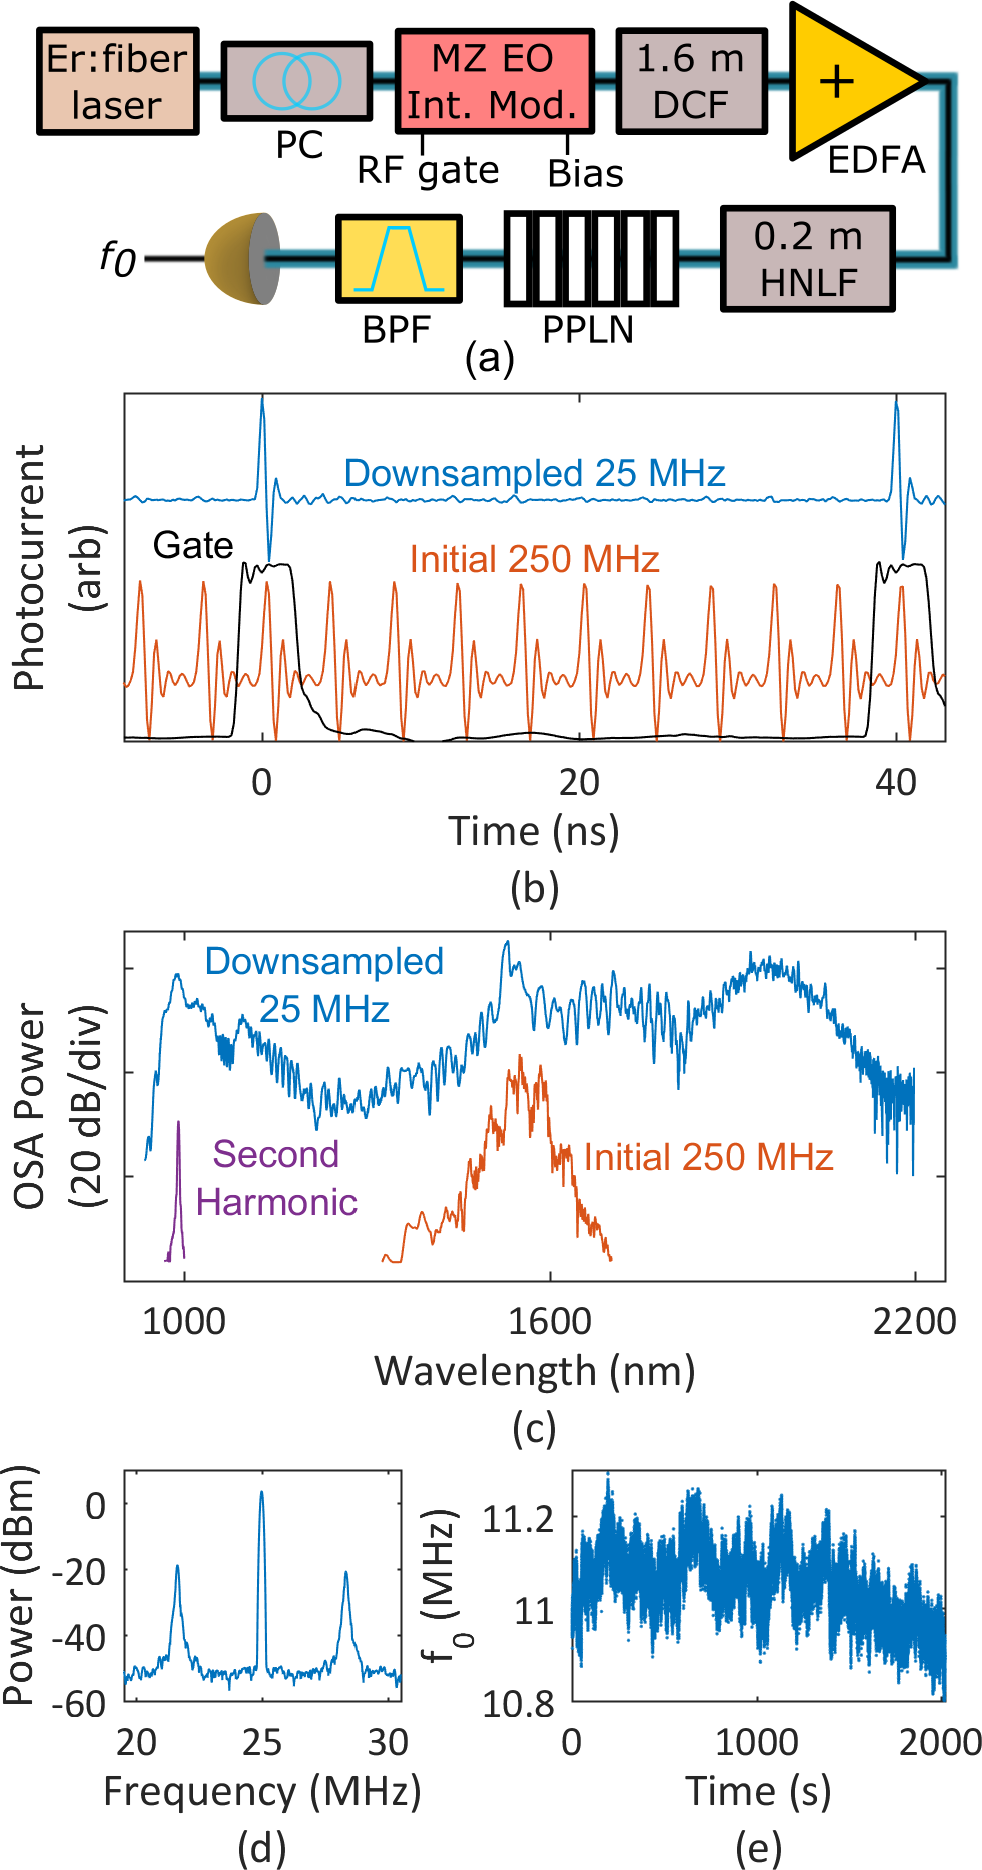
\includegraphics[width=110mm]{\FigPath/Figures/PulsePicking/PulsePickingPaperFig1.png}
		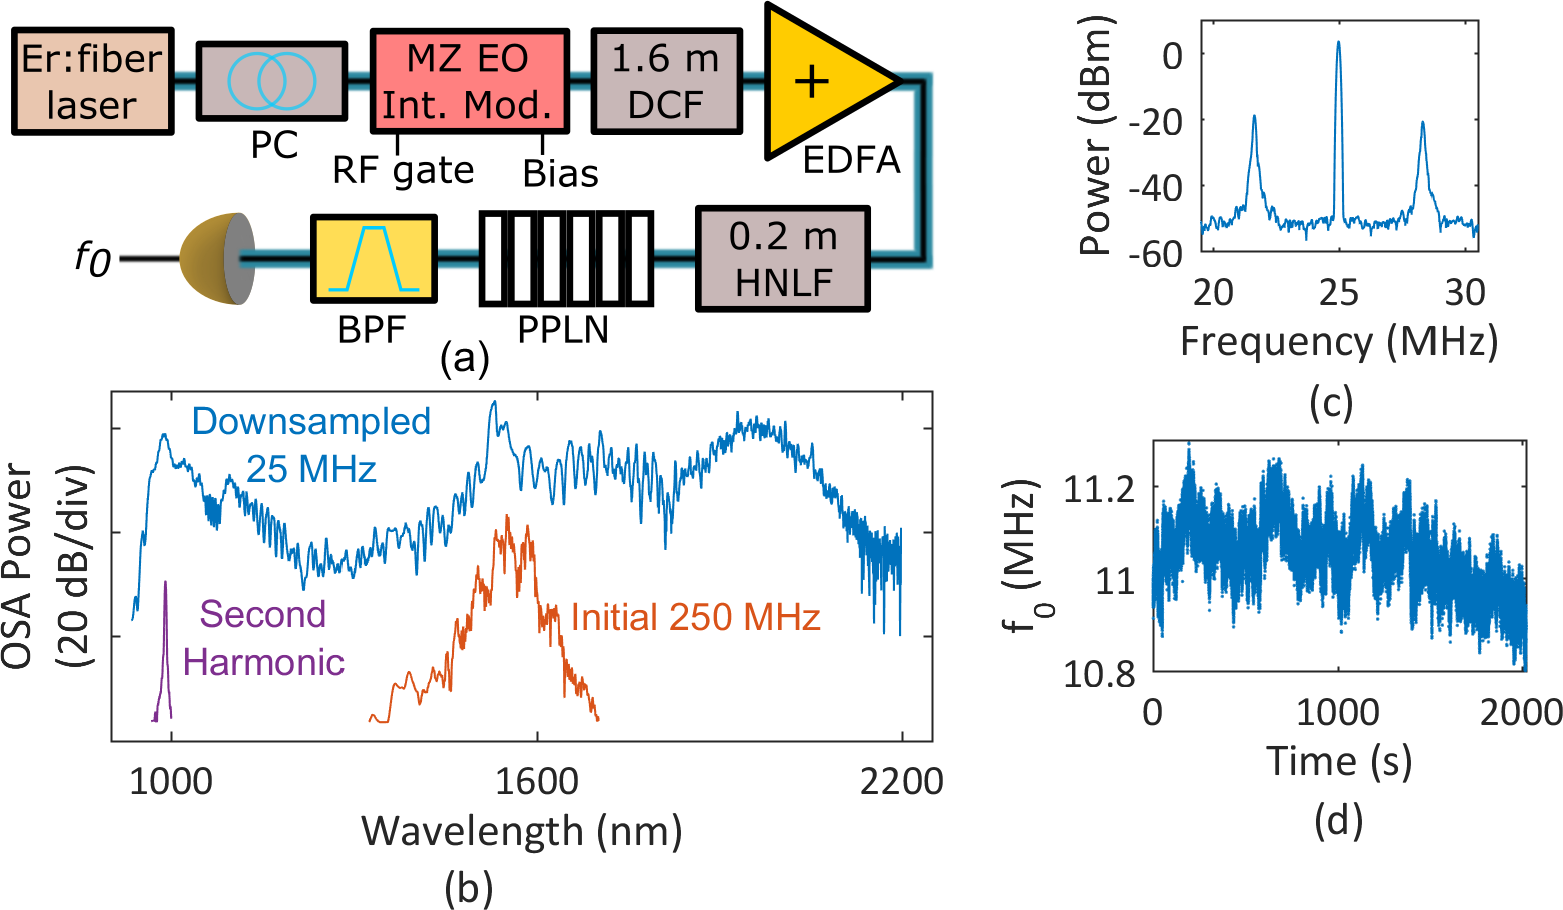
\includegraphics{\FigPath/Figures/PulsePicking/PPProofOfConceptFigv2.png}
	\end{center}
	\caption[Demonstration of downsampling for $f_0$ detection]{\textbf{Demonstration of downsampling for $f_0$ detection.} (a) Schematic depiction of the setup for downsampling a 250 MHz Er:fiber comb and detecting the offset frequency of the resulting 25 MHz pulse train. PC---polarization controller.  DCF---dispersion-compensating fiber. EDFA---erbium-doped fiber amplifier. HNLF---highly nonlinear fiber. PPLN---periodically-poled lithium niobate. BPF---(optical) band-pass filter. (b) Octave-spanning supercontinuum generated by downsampling (top, blue), second harmonic generated for $f_0$ detection (purple), and for comparison the supercontinuum generated by the same apparatus without downsampling (orange). (c) Detected repetition rate and $f_0$ beat at 100 kHz resolution bandwidth; signal-to-noise ratio of $f_0$ is 30 dB. (d) Counted frequency of the detected free-running offset beat. Data is taken for $\sim$2000 s at 10 ms gate time. The offset frequency of the 250 MHz commercial comb was adjusted between measurements shown in Figs. \ref{fig:PPDemo}c and \ref{fig:PPDemo}d to simplify electronic processing.}
	\label{fig:PPDemo}
\end{figure} 



\section{Mathematical model for downsampling}\label{sec:PPMath}
While Fig. \ref{fig:PPDemo} presents an absolute frequency measurement of $f_0$ enabled by downsampling, it does not demonstrate the deterministic connection between the input and downsampled combs that is essential for applications. To understand this relationship, we first consider a simple model of downsampling, and then discuss experimental tests of its conclusions.

The downsampled pulse train's electric field is modeled as the product of the incoming comb's field and a time-varying amplitude modulation. For an incoming optical frequency comb with repetition rate $f_{rep}$, complex single-pulse field $A(t)$ that is localized near $t=0$, and pulse-to-pulse carrier-envelope phase shift $\phi$, pulse gating by a train of rectangular pulses of length $t_g$ and arrival rate $f_g$  yields a downsampled comb with field
\begin{equation}
a(t)=\left[\Sigma_n A(t-n/f_{rep}) e^{in\phi}\right]\times\left[\Sigma_m \mathrm{Rect}\left((t-m/f_g)/t_g \right)\right]  \label{eq:PPmathResult1}
\end{equation}                                            
where $\mathrm{Rect}(x)$ is the rectangle function, taking the value 1 for $-1/2\leq x\leq 1/2$ and 0 elsewhere. Indices $n$ and $m$ count the pulse number of the incoming pulse train and the electronic gate respectively. The optical spectrum of the downsampled pulse train $a(t)$, calculated via the convolution theorem for the Fourier transform, is:
\begin{equation}
\mathcal{F}\{a\}(f)\sim 4\pi f_{rep} \Sigma_{nm}\frac{1}{m}\mathcal{F}\{A\}(f_0+nf_{rep})\times\mathrm{sin}(\pi m t_g f_g)\delta(f-f_0-nf_{rep}-mf_g ),
\end{equation}
where $f_0=f_{rep}\cdot\phi/2\pi$ is the carrier-envelope offset frequency of the incoming comb and $\delta$ is the Dirac delta function.  The downsampled pulse train has spectral content at optical modes $f_0+nf_{rep}$, as well as at intensity modulation sidebands whose frequency offsets $mf_g$ are harmonics of the gating frequency. To avoid the generation of unwanted modulations, pulse gating at an integer sub-harmonic of the incoming repetition rate, $f_g=f_{rep}/N$, is essential. In this case superposition of the intensity modulation components created by pulse gating results in a downsampled frequency comb with a single mode spacing. Moreover, this model predicts that the offset frequency is preserved up to a reduction modulo the comb's new repetition rate. 

Notably, for pulse gating at a sub-harmonic of the input comb's repetition rate, timing jitter of the electronic gate that is less than its duration does not contribute to noise on the downsampled comb. By modeling jitter as gate-to-gate arrival-time delays $\Delta t_m$, it can be shown that the downsampled comb's amplitude $a(t)$ and spectrum $F\{a\}(f)$ do not deviate from Eq. \ref{eq:PPmathResult1} provided that: (1) The jitter is a sufficiently small $|\Delta t_m |<t_g/2$, i.e., that the optical and electronic pulses are always substantially overlapped, and (2) That the optical pulses are substantially shorter than the electrical pulses, which is true for most systems. Thus, in general we expect that the carrier-envelope offset frequency of the incoming comb is preserved by downsampling even with jitter on the gate signal. 

\section{Experimental investigation of the effect of downsampling on the pulse train's noise properties}\label{sec:PPNoiseExp}
We supplement the mathematical model presented above with an experimental investigation of the effects of downsampling on the noise properties of the pulse train. First we consider the effects of technical limitations to ideal downsampling, and then we discuss fundamental effects associated with aliasing of high-Fourier-frequency optical noise and shot noise. 

We measure the phase-noise spectrum of the downsampled comb's repetition rate at different points in our apparatus, as shown in Fig. \ref{fig:PPNoiseExp}a. We also plot the phase noise of the 250 MHz comb, which has been shifted by $-10 \mathrm{log}_{10}(N^2)=-20$ dB to facilitate comparison \cite{Mandridis2010}, and the phase noise of the electronic gate. The downsampled frequency comb's phase-noise spectrum matches that of the 250 MHz comb except for a small increase at $\sim$3 kHz, likely corresponding to the corner in the gate generator's phase noise at the same frequency. The phase noise of the high- and low-frequency ends of the supercontinuum similarly matches the 250 MHz comb below 1 kHz.  The higher phase noise in the supercontinuum beyond 1 kHz is above the measurement system's noise floor (including shot noise), despite the reduced optical power available after spectral filtering. This higher noise is likely due to noise generation processes in the HNLF, such as the conversion of amplitude fluctuations on input pulses to timing jitter in the supercontinuum \cite{Dudley2006}.

\begin{figure}[htpb]
	\begin{center}
		%		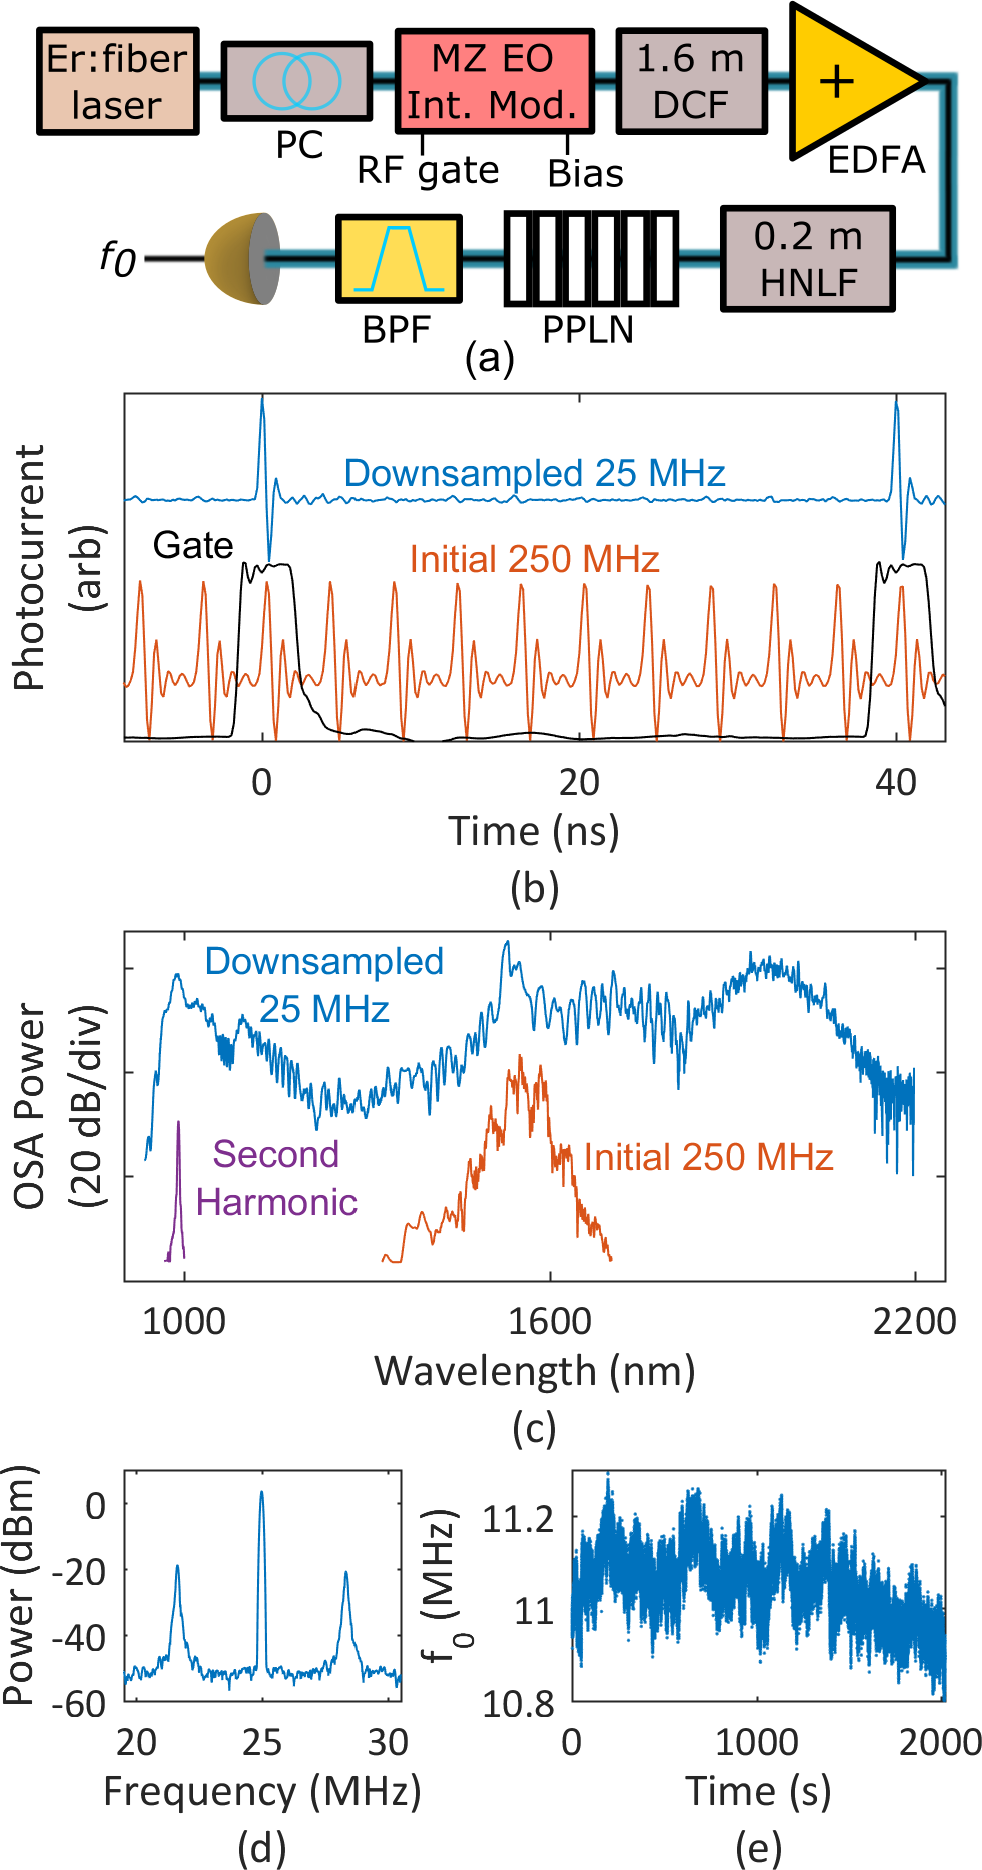
\includegraphics[width=110mm]{\FigPath/Figures/PulsePicking/PulsePickingPaperFig1.png}
		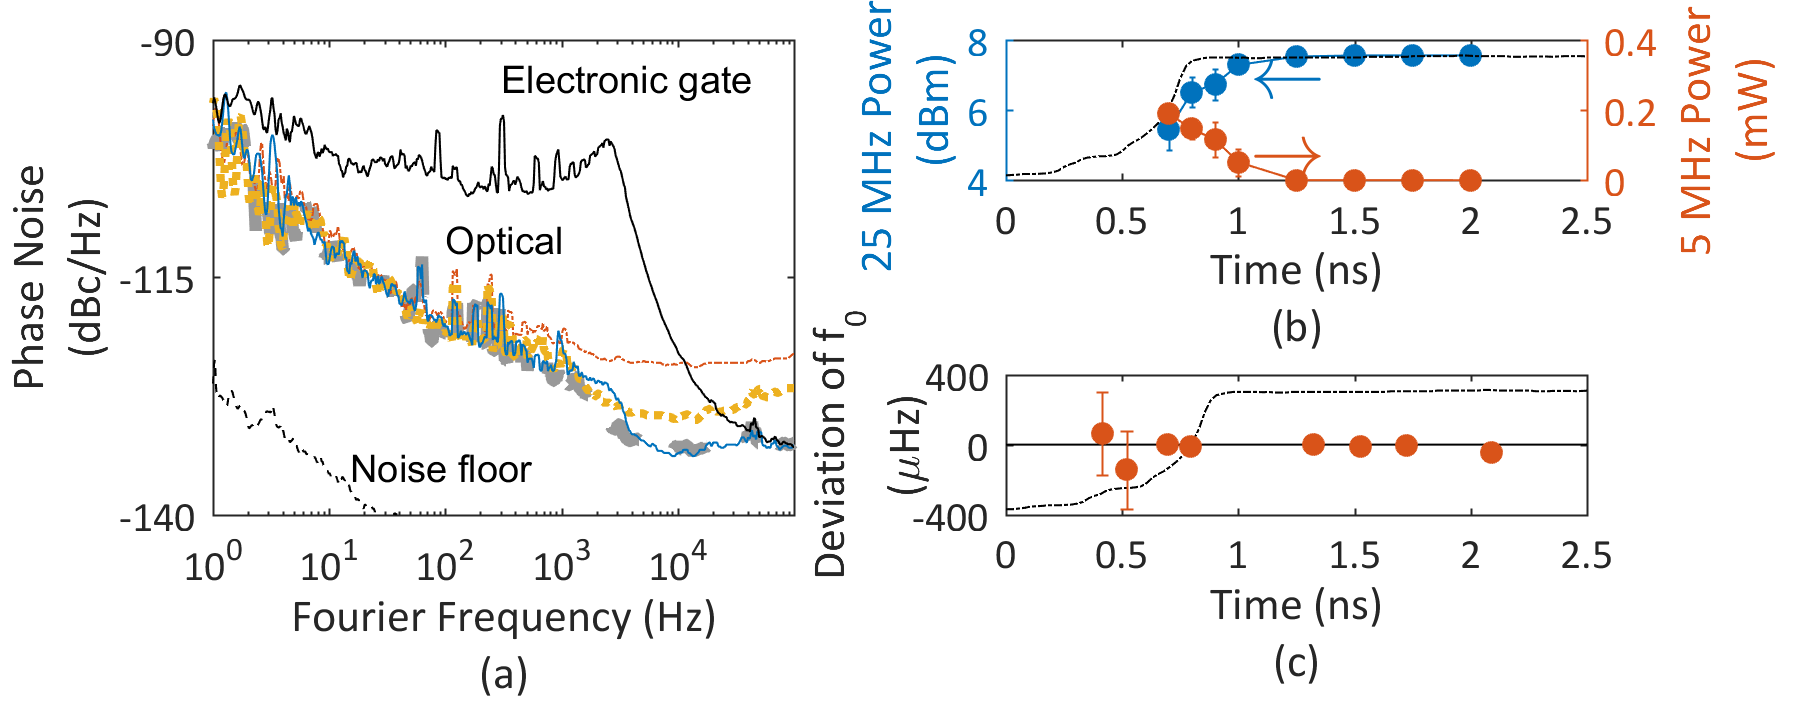
\includegraphics{\FigPath/Figures/PulsePicking/Fig2_thesis.png}
	\end{center}
	\caption[Experimental investigation of noise introduced by downsampling]{\textbf{Experimental investigation of noise introduced by downsampling.} (a) Measured repetition-rate phase noise of spectral components of the supercontinuum, selected by a 990$\pm$5 nm band-pass filter (dot-dashed orange), 1650 nm long pass filter (dotted yellow), and the entire downsampled 25 MHz frequency comb measured immediately before the EDFA (solid blue), the 250 MHz comb (large-dashed gray, shifted by $20\,\mathrm{log}(1/10)=-20$ dB). Also shown is the phase noise of the electronic gate generator (top, solid black). (b) Amplitude of the downsampled pulse-train modulation due to 250 ps jitter at 5 MHz rate. The position of a data point on the x-axis indicates its mean position within the gate, shown in dashed black. Measurement uncertainties arise due to a latency between the optical trigger and the start of the electronic gating signal which varies on the order of 50 ps. (c) Deviation of the carrier-envelope offset frequency of the downsampled comb from the 250 MHz comb's offset frequency as a function of the alignment of optical pulses within the gate.}
	\label{fig:PPNoiseExp}
\end{figure} 

The timing jitter of our gating pulse train is between 5 ps (obtained by integrating the phase noise plotted in Fig. \ref{fig:PPNoiseExp} to 100 kHz) and 10 ps (extrapolating constant phase noise to the 12.5 MHz Nyquist frequency and integrating). These jitter values are small relative to the 4 ns repetition period of the incoming optical pulse train. As the repetition rate of the incoming optical pulse train increases to $>$10 GHz, the gate duration must correspondingly decrease for single-pulse gating, and timing jitter on the gate may become a significant fraction of the gate duration. To explore the effects of timing jitter larger than our pulse generator's inherent 5 to 10 ps, we impose excess jitter on the gating signal. We modulate the relative timing between the gating signal and the incoming optical pulse train at a frequency of 5 MHz with an amplitude of 250 ps. The effect of this jitter is manifest in the microwave power of the gated comb as 5 MHz intensity-modulation sidebands whose amplitude depends on the position of the optical pulses within the gate, as shown in Fig. \ref{fig:PPNoiseExp}b.  Pulses with a mean position within 250 ps of the gate edge are substantially modulated by the 5 MHz gate-delay signal. This agrees with the prediction of a sharp threshold on the acceptable level of timing jitter on the gate.

It is essential to establish that the comb's carrier-envelope offset frequency is preserved in the downsampling process. To do this, we perform a frequency comparison of the 25 MHz downsampled comb and a separate output of the 250 MHz comb. This 250 MHz output is intensity modulated so that a measurement of the nonzero optical heterodyne beat frequency between an intensity modulation sideband and a pulse-gating sideband of the downsampled comb reveals the relative frequency offset of the two combs. Figure \ref{fig:PPNoiseExp}c shows the null frequency shift between the 25 MHz and 250 MHz combs, which we have characterized for different alignments of the optical pulse within the gate. At the level of several microhertz, better than $10^{-18}$ relative to the 200 THz optical carrier frequency, we observe no frequency shift between the 250 MHz comb and the downsampled 25 MHz comb when the gate is properly aligned. This confirms the utility of downsampling for measurement of a high-repetition-rate comb's offset frequency for subsequent use of the comb in, for example, a spectroscopy experiment requiring high power per comb mode and high frequency precision.

\section{Effects of ideal downsampling on a pulse train's noise properties}\label{sec:PPNoiseTheory}

In addition to the conversion of electronic technical noise to optical noise on the downsampled pulse train, there exists a further mechanism by which downsampling can change the measured amplitude noise properties of the pulse train. Even ideal downsampling, free of electronic noise, leads to an increase in the measured power spectral density (PSD) of optical pulse energy fluctuations (PEF) when technical pulse energy noise is present. This is due to aliasing of components of the PSD of pulse energy fluctuations at frequencies above the Nyquist frequency of the downsampled pulse train $f_{rep}/2N$ but below the Nyquist frequency of the original pulse train $f_{rep}/2$. Assuming random fluctuations from pulse to pulse, downsampling does not change the RMS fractional pulse energy fluctuation $\sigma_{PEF}$, whose square is equal to the frequency integral of the PSD of pulse energy fluctuations $S_{PEF} (f)$:
\begin{equation}
\sigma_{PEF}^2=\int_{0}^{f_{rep}/2}df S_{PEF} (f).         
\end{equation}
                       
Because the Nyquist frequency defines the upper limit for integration of $S_{PEF}$, in order for $\sigma_{PEF}$ to be preserved $S_{PEF}(f)$ must increase when the Nyquist frequency is reduced by downsampling. For example, in the simple case of white technical noise on the pulse energies with density $S_o$, we have

\begin{equation}
\sigma_{PEF}^2=\int_{0}^{f_{rep}/2}df S_o=\int_{0}^{f_{rep}/2N}df S^{'}
\end{equation}
which shows that downsampling must increase the measured PSD of white technical noise from $S_o$ to $S^{'}=NS_o$, assuming there are no spectral correlations. However, this simple multiplicative increase is restricted to the case of white technical noise. In general, the PSD of pulse energy fluctuations of the new pulse train is determined from the original PSD through the usual method of modeling aliasing of a signal: a new Fourier frequency for each component of the original PSD is obtained by reducing the original Fourier frequency by a multiple of $-f_{rep}/N$ so that it lies between $-f_{rep}/2N$ and $f_{rep}/2N$ and taking its absolute value. The new PSD is then determined by taking the quadrature sum of the PSD components at the same aliased Fourier frequency. This phenomenon is derived mathematically and demonstrated experimentally in Ref. \cite{Gohle2005}, where the analysis of carrier-envelope phase noise applies equally well to pulse energy fluctuations. 

In contrast with the increase in the PSD of pulse energy fluctuations arising from coincidence of the optical pulse with the edge of the electrical gate, which increases $\sigma_{PEF}$, the aliasing mechanism described above preserves $\sigma_{PEF}$. An important consequence of this is that while technical noise can lead to supercontinuum decoherence in external nonlinear spectral broadening, aliasing does not, because it is $\sigma_{PEF}$ which determines the degree of supercontinuum decoherence. Thus the aliasing mechanism impedes $f-2f$ self-referencing only by reducing the available signal-to-noise ratio of an $f_0$ signal in a straightforward linear fashion. 

In practice, the relevance of the aliasing of the PSD of pulse energy fluctuations is determined by the presence of technical noise on the pulse energies at high Fourier frequency $f > f_{rep}/2N$. For sufficiently small downsampling factors (e.g. $f_{rep}/2N\geq\sim50$ MHz) and depending on the comb source, it is possible that the only source of intensity noise at frequencies above $f_{rep}/2N$ is shot noise. Shot noise results in a maximal (shot-noise-limited) signal-to-noise ratio (SNR) of an optical heterodyne beat with a local oscillator laser which is reduced by $N^2$ (in electrical power units) as the average power of the pulse train is reduced by downsampling by a factor of $N$. In contrast, in the case of detection of a carrier-envelope-offset beat with fixed optical detection bandwidth, the shot-noise-limited SNR is preserved in downsampling. One way to understand these results is to model the shot noise at a given Fourier frequency as the incoherent sum of optical heterodyne beats between each optical comb mode and the uncorrelated vacuum fluctuations at the appropriate optical frequency \cite{Bachor1990,Quinlan2013}, and to take into account the fact that during downsampling the optical power of each comb mode is reduced by $N^2$, with the first factor of $N$ coming from reduction of the total optical power and the second factor of $N$ due to the increase in the spectral density of comb modes. 

We experimentally investigate the impact of downsampling on the PSD of pulse energy fluctuations by measuring noise on three photodetected optical signals: a shot-noise-limited telecommunications-band CW laser, a 10 GHz pulse train generated by passing this laser through cascaded optical phase and intensity modulators (see Chapter \ref{chap:EOMCombs} and Ref. \citeNoBrackets{Cole2016}) and then a low-noise EDFA, and this pulse train after downsampling by a factor of four to 2.5 GHz repetition rate with no additional amplification after downsampling. Shown in Figure \ref{fig:PPSNComparison} are curves for each signal of the fluctuations $\sqrt{S_I (f=50\, \mathrm{MHz})}$ in the detected photocurrent at a Fourier frequency of 50 MHz versus the total time-averaged detected photocurrent $\left<I\right>$ from the optical signal. To measure the scaling of noise with optical power, these curves are generated by beginning with an optical signal that yields more than 800 $\mathrm{\mu}$A of detected photocurrent and attenuating this signal before photodetection. The data indicate that both the pulse-generation process and the downsampling process contribute some amount of technical noise at 50 MHz Fourier frequency to the photocurrent, because the measured curves are well-modeled by a quadrature sum of a shot-noise contribution and a technical noise contribution. The contributions of these two types of noise can be determined because they scale differently with the photodetected power: shot noise obeys the relationship  $\sqrt{S_I (f=50\, \mathrm{MHz})}=\sqrt{2e\left<I\right>}$, $\left<I\right>$ denoting the time-averaged photocurrent, while the technical-noise contribution arises from fluctuations in the expected photocurrent $I(t)$  and scales linearly with the detected photocurrent. We observe that downsampling by a factor of four leads to a multiplication of the amplitude of the technical noise by a factor of $\sim$1.7 on the optical signal relative to the carrier, which due to finite noise bandwidth is somewhat less than the factor of two (four, in electrical power units) that would be expected for ideal downsampling by a factor of four in the presence of white technical noise. These results further demonstrate that, properly implemented, downsampling does not magnify noise on the pulse train to a degree that is prohibitive for applications.

\begin{figure}[htpb]
	\begin{center}
		%		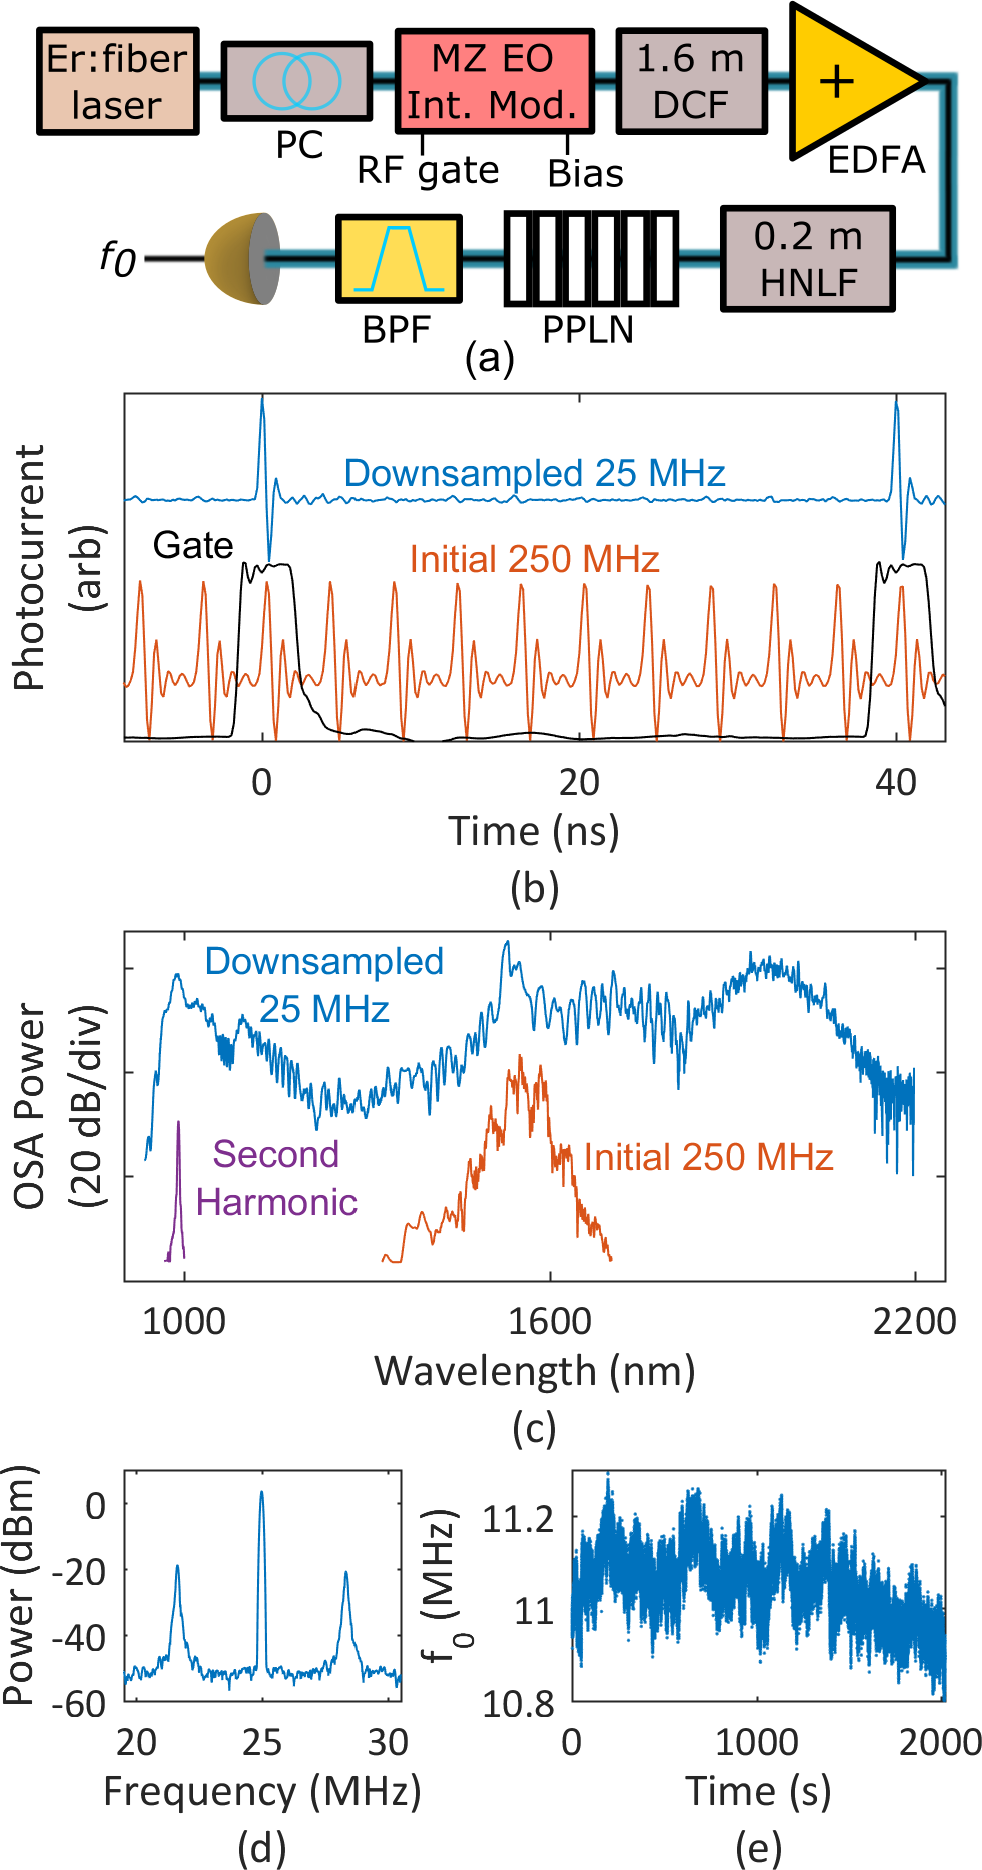
\includegraphics[width=110mm]{\FigPath/Figures/PulsePicking/PulsePickingPaperFig1.png}
		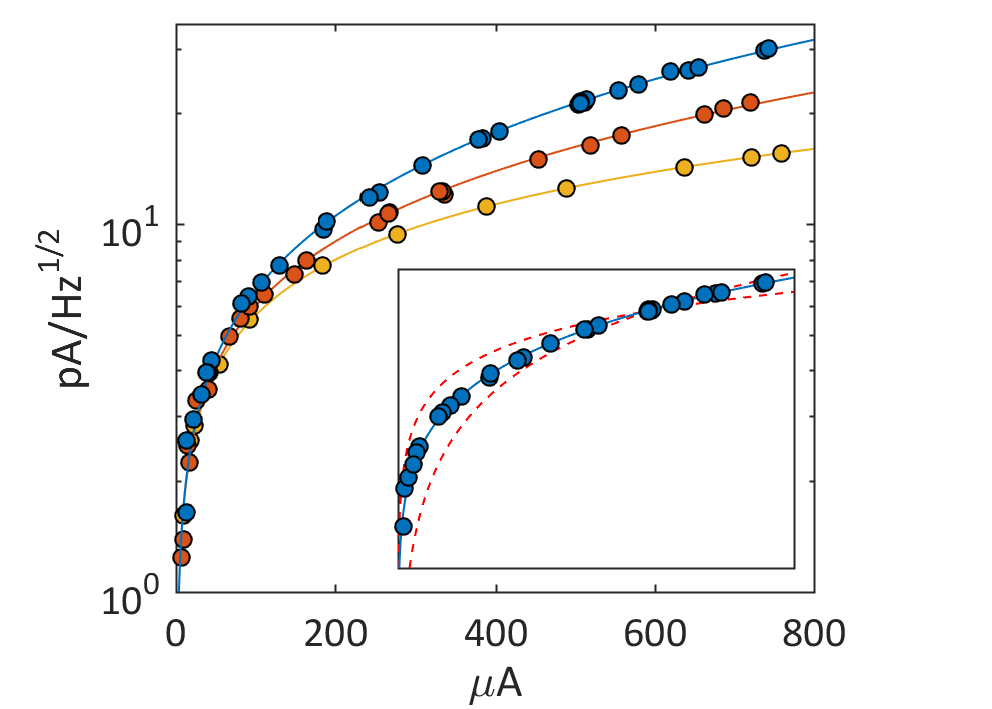
\includegraphics{\FigPath/Figures/PulsePicking/PPSNComparison.png}
	\end{center}
	\caption[Effect of downsampling on photocurrent fluctuations]{\textbf{Effect of downsampling on photocurrent fluctuations.} Fluctuations at 50 MHz Fourier frequency in the detected photocurrent as a function of the time-averaged photocurrent in three cases: CW laser at the shot-noise limit (lowest, yellow), 10 GHz pulse train (middle, red), and 2.5 GHz downsampled pulse train (highest, blue). Dots show measured data and curves show fits to the data. The fit for the shot-noise-limited laser has a single free parameter, which is a scaling factor of order 1 due to frequency dependence of the photodetector's transimpedance gain. The fits for the pulse trains have a scaling factor in common, and have as an additional parameter the amplitude of the technical noise on the pulse train. This is -153.9 dBc/Hz for the 10 GHz pulse train and increases by a factor of $\sim$1.72 to -149.3 dBc/Hz for the 2.5 GHz downsampled pulse train. Inset: Optimized fits (dashed red) to the experimental data for the downsampled 2.5 GHz pulse train using only shot noise or linear technical noise scaling, demonstrating that both noise processes are important for explaining the data. }
	\label{fig:PPSNComparison}
\end{figure} 

\section{Model for the effect of incomplete extinction of rejected pulses and amplification of a downsampled pulse train}\label{sec:PPAmplification}
To this point, we have considered effects of downsampling assuming that extinction of the rejected pulses is complete, but in a practical application this will not necessarily be the case.  The modulators used for pulse extinction may transmit a substantial amount of energy from the rejected pulses---for example, one commercial manufacturer specifies 25 dB extinction ratio, and this number can vary in practice. Additionally, the electronic gating signal may not have sufficient bandwidth to completely switch from transmission to extinction within the repetition period of the incoming pulse train, and initial extinction can be followed by some transmission caused by ringing in the gating signal. Bandwidth limitations will be increasingly likely as the repetition rates of frequency combs increase, placing more demanding requirements on gating electronics.  Incomplete extinction will add modulations to the optical spectrum and will raise the total power of the downsampled pulse train while keeping the energy of the fully-transmitted pulses fixed. This will require higher average power to achieve a given target pulse energy.

The effects of incomplete extinction of rejected pulses are exacerbated if the incomplete extinction does not happen in a deterministic and repetitive fashion; this could occur, for example, if intermediate pulses fall near the edge of the gate in the presence of relative timing jitter between the optical and electronic pulse trains, or if the extinction ratio fluctuates in time. Interestingly, if the downsampled pulse train is subsequently amplified and spectrally broadened, the impact of incomplete extinction depends on whether the optical amplifier used operates in the linear regime or in the saturated regime.

As an example, we consider the case where each fully transmitted pulse is preceded and followed by partially-extinguished pulses whose amplitudes fluctuate for each period of the downsampled pulse train. This fluctuation could occur because the pulses lie on the edge of the electronic gate and there is relative timing jitter between the optical pulse train and the gating signal. It is true that these fluctuations will lead to decoherence during nonlinear spectral broadening. However, the coherence is degraded by this mechanism only within the bandwidth that is achieved by the broadened, partially-extinguished pulses. In efficient $f-2f$ interferometry only the fully-transmitted pulses should reach an octave in bandwidth.  Therefore, this mechanism of supercontinuum decoherence is not a problem in $f-2f$ interferometry in general, unless there is coupling between the amplitudes of the amplified partially-extinguished pulses and the amplified fully-transmitted pulses. This coupling can arise, for example, through amplification in the saturation regime, which then leads to decoherence across the full bandwidth of the supercontinuum. 

To illustrate this point, we have performed numerical simulations of the spectral broadening of a 100 GHz train of 100 fs pulses that has been downsampled to 10 GHz and then amplified. We use an adaptive \cite{Heidt2009} split-step Fourier method \cite{Hult2007} to simulate spectral broadening in 30 cm of HNLF according to the generalized nonlinear Schrodinger equation \cite{Agrawal2007} (see Appendix \ref{app:numericalsims}). In the simulation each fully-transmitted pulse, amplified to 1 nJ, is preceded and followed by partially-extinguished pulses with normally distributed and uncorrelated energies with mean of 0.3 nJ and standard deviation of 0.225 nJ. This models the effect of adjacent pulses that coincide with the edge of the gate. We simulate amplification in two regimes: saturation is simulated using a fixed-energy method wherein the pulse energies in each three-pulse burst are rescaled by a common factor so that the total energy is 1.6 nJ; linear amplification is simulated using a fixed-gain model, which involves no such rescaling of pulses. Numerically, we simulate the spectral broadening of each pulse individually, which is acceptable because terms in the generalized nonlinear Schrodinger equation operate only locally or, in the case of the Raman term, on the timescale of several femtoseconds, while the separation between the pulses in each burst is 10 ps (the inverse of the initial 100 GHz repetition rate).  We have verified that during simulated time-evolution each broadened pulse remains well-centered in its 5 ps simulation window. 

Results of this study are shown in Figure \ref{fig:PPAmp}. Figure \ref{fig:PPAmp}a depicts a three-pulse burst before and after propagation in HNLF. In Figure \ref{fig:PPAmp}b we show spectra corresponding to spectral broadening of this three-pulse burst, as well as plots of the spectral coherence averaged over many simulations. The first-order spectral coherence $g_{12}^{(1)} (\lambda)$ is defined as:
\begin{equation}
\left|g_{12}^{(1)} (\lambda)\right|=\left|\frac{\left<E_1^*(\lambda)E_2(\lambda)\right>}{\sqrt{\left<|E_1(\lambda)|^2\right>\left<|E_2(\lambda)|^2\right>}}\right|=\left|\frac{\left<E_1^*(\lambda)E_2(\lambda)\right>}{\left<|E(\lambda)|^2\right>}\right|.
\end{equation}

Curves are plotted for the fixed-gain and fixed-energy cases, as well as for the case with ideal downsampling (no partially-extinguished pulses) and only shot-noise on the pulse train. The averages in the formula above are over 1000 instantiations of the pair $E_1$ and $E_2$, for a total of 2000 broadened spectra for each pulse within the burst of three. In both the fixed-gain and fixed-energy cases the coherence is poor in the center of the spectrum, but in the fixed-gain case, which models amplification in the linear regime, the coherence is preserved in the high- and low-frequency ends of the spectrum where it is needed for self-referencing.

\begin{figure}[htpb]
	\begin{center}
		%		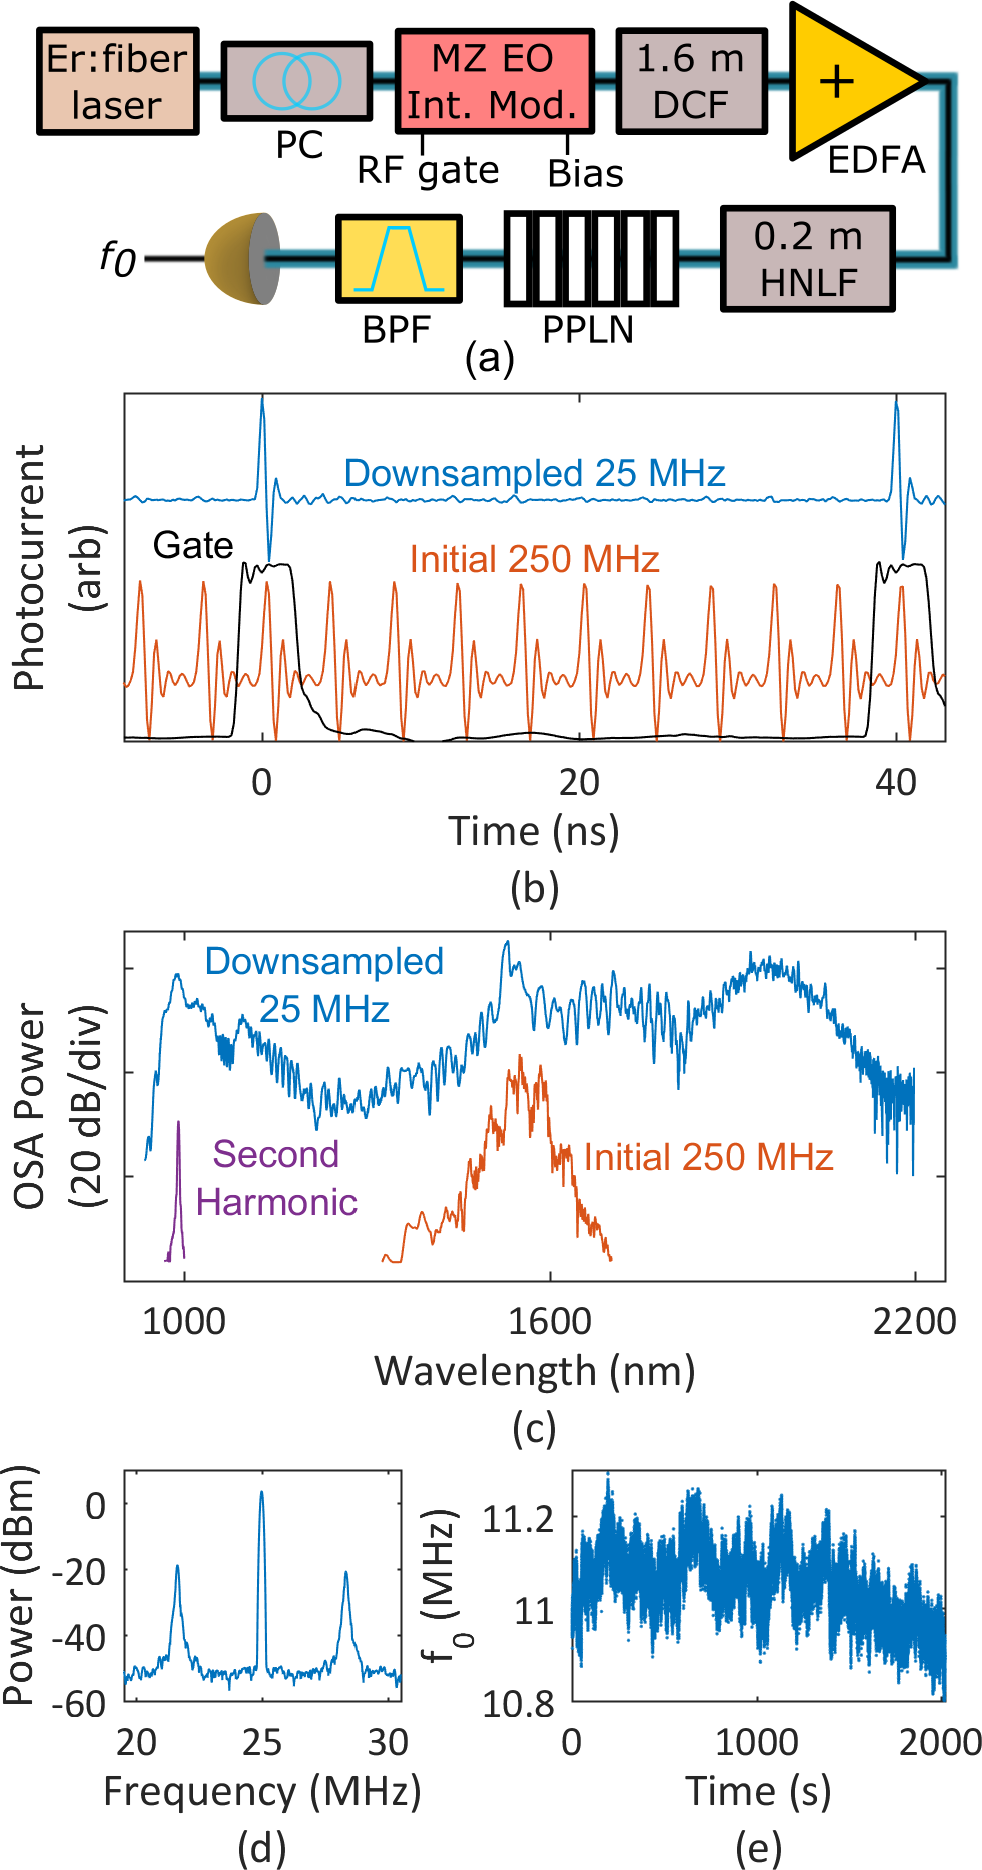
\includegraphics[width=110mm]{\FigPath/Figures/PulsePicking/PulsePickingPaperFig1.png}
		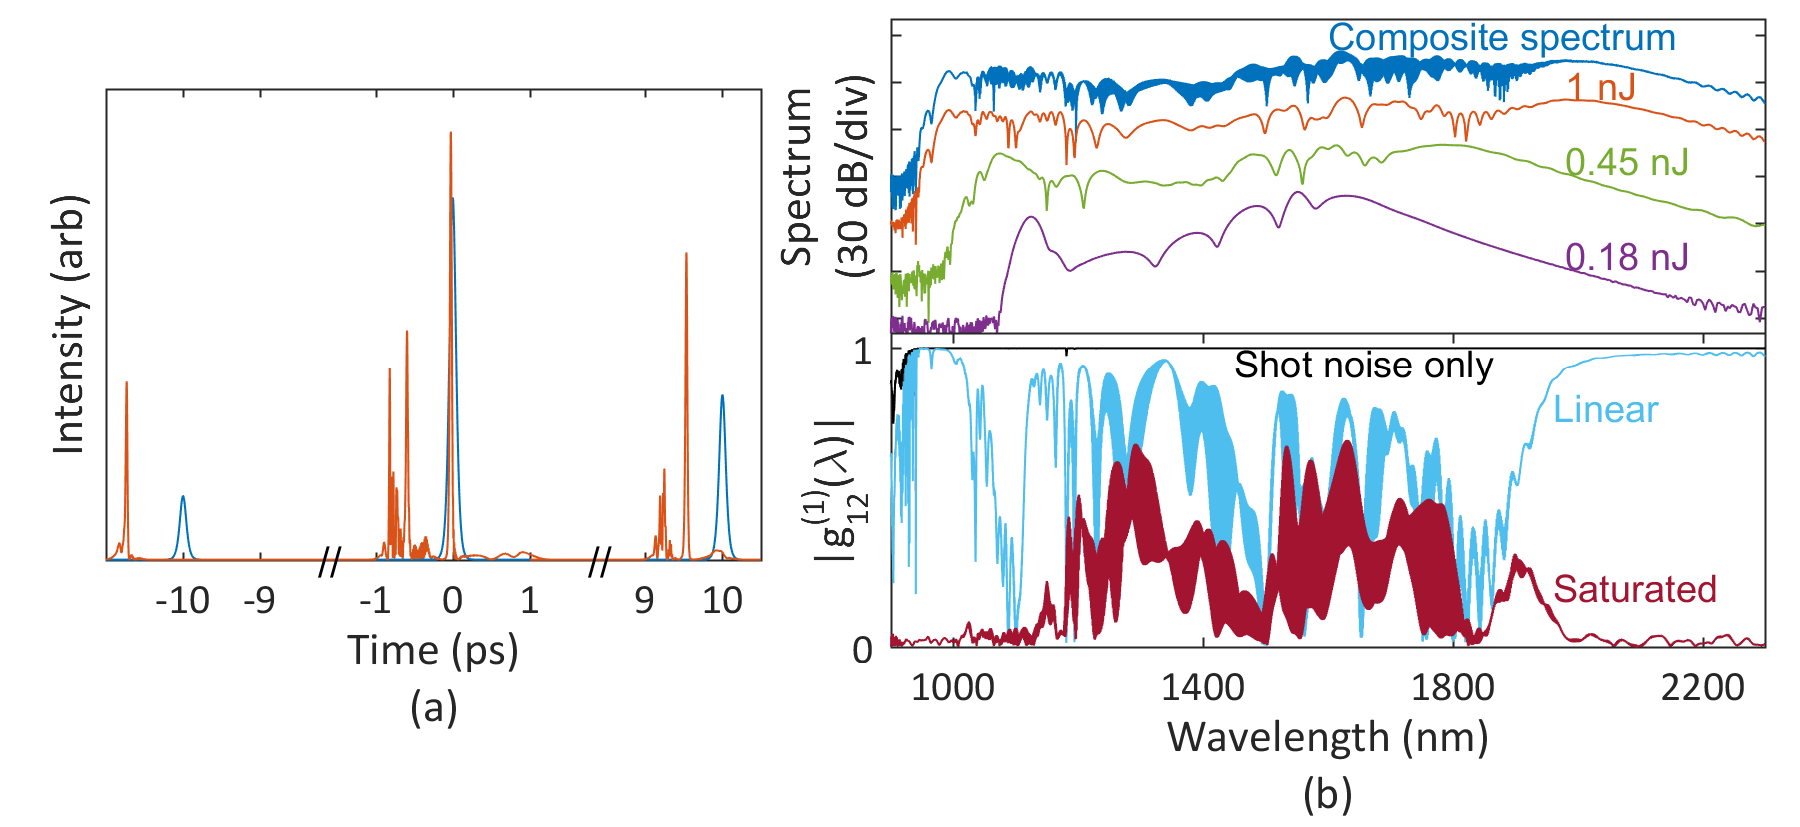
\includegraphics{\FigPath/Figures/PulsePicking/PPAmp.png}
	\end{center}
	\caption[Investigation of incomplete pulse extinction and amplification]{\textbf{Investigation of incomplete pulse extinction and amplification.} (a) A burst consisting of a fully-transmitted 1 nJ, 100 fs pulse and 100 fs partially-transmitted adjacent pulses with energies of 0.18 nJ and 0.45 nJ. Blue indicates initial $\mathrm{sech}^2$ pulses, and orange indicates the intensity after propagation through 30 cm HNLF. Note that the $x$-axis has been broken. (b) Top panel: optical spectra corresponding to the pulses shown in orange in (a), showing the composite spectrum of the three pulses (top, blue) and the spectra of the 1 nJ central pulse (second, orange), the 0.45 nJ adjacent pulse (third, green), and the 0.18 nJ adjacent pulse (bottom, purple). Bottom panel: Calculated spectral coherence averaged over 2000 simulations for the case of shot noise only (top, black) and for the case of fluctuating amplitudes of the first and third pulses as described in the text, after simulated amplification in a linear-regime optical amplifier (second, teal), and a saturated optical amplifier (bottom, maroon).  For the case of linear-regime operation, high spectral coherence is preserved in the extreme ends of the supercontinuum even as it is lost in the center, in contrast with the complete loss of coherence after amplification in saturation. 
	\label{fig:PPAmp}}
\end{figure} 

\section{Further remarks on the application of downsampling}\label{sec:PPConclusion}
Downsampling via pulse gating is a promising tool to manipulate high repetition-rate frequency combs from low size, weight, and power packages and to aid in the detection of their offset frequencies. In our experiments downsampling enabled detection of $f_0$ at a signal-to-noise ratio sufficient for measurement and stabilization, which otherwise would have required significantly higher average power. The effects of the electronic timing jitter of the gate signal are negligible so long as incoming optical pulses do not arrive coincidentally with the edge of the gate; when they do, timing jitter induces amplitude noise on the transmitted pulses. This results in an increase in RMS optical pulse energy fluctuations $\sigma_{PEF}$. Independently, the PSD of pulse energy fluctuations may be increased by aliasing of technical noise and by shot noise, depending on the relative magnitudes of these two types of noise. Each of these sources of signal-to-noise-ratio degradation has the potential to interfere with detection of $f_0$. This investigation of these challenges will facilitate application of the technique in high repetition-rate frequency comb systems. Importantly, our experiments demonstrated that downsampling does not add a significant amount of noise to the frequency components of the pulse train, and in a separate experiment the technique has recently been used successfully to detect the carrier-envelope offset frequency of a 10 GHz comb by downsampling by a factor of four (\cite{Beha2017}, see Chapter \ref{chap:EOMCombs}).

To employ downsampling as demonstrated here with repetition rates $>$10 GHz will require electronic gates with duration $\leq$100 ps. Technology to downsample with gates as short as 20 ps is commercially available, while 100 Gb$/$s integrated circuits and 25 GHz demultiplexing have been demonstrated \cite{Driad2011,Ferenci2012}, and this technology continues to improve. Barring the use of such state-of-the-art electronics, pulse gates of duration longer than the incoming optical pulse train's repetition period can be employed.  This will be technically easier to achieve, but will result in additional modulations on the spectrum of the downsampled pulse train.

The ambiguity of the input comb's offset frequency as a result of the reduction of the offset frequency modulo the new repetition rate makes downsampling most suitable for applications where the ambiguity can be removed by some other method.  Two such applications are frequency comb calibration of astronomical spectrographs, where measurement of the wavelength of a comb mode can remove the ambiguity, and microresonator-based frequency combs, where the uncertainty in the offset frequency is determined by the frequency stability of the pump laser and can be much less than the repetition rate of the downsampled comb. 







\appendix
%\chapter{Derivation of the Lugiato-Lefever equation from the nonlinear Schrodinger equation}
 \label{app:LLEfromIkeda}


Here we show how the Lugiato-Lefever equation can be obtained by modeling propagation in a high-finesse ring cavity with the nonlinear Schrodinger equation and periodically applying an operator that implements in-coupling and out-coupling, including the effects of the round-trip phase shift associated with the detuning of the pump laser from a cavity mode. To my knowledge, the derivation given here was first performed by Haelterman, Trillo, and Wabnitz \cite{Haelterman1992a}. We use the NLSE for a pulse of restricted bandwidth such that higher-order nonlinearities are unimportant, but this derivation may also be carried out using a generalized nonlinear Schrodinger equation to include higher-order effects (e.g. Raman and self-steepening) in the LLE. Our equation is:


\begin{equation}
\frac{\partial A}{\partial z}= -\frac{\alpha_\ell}{2} A+i\gamma|A|^2 A -i \frac{k''}{2} \frac{\partial^2 A}{\partial T^2}. \label{eq:NLSEloss}
\end{equation}

This equation is ubiquitous in the study of pulse propagation in Kerr-nonlinear media, and a derivation of it is provided, for example, in Ref. \cite{Agrawal2007}. As discussed in Sec. \ref{sec:solitonmath}, it describes the evolution of a pulse envelope $A$ in a `fast-time' reference frame parametrized by $T$ as it propagates in a Kerr-nonlinear medium, where the propagation distance is parametrized by the variable $z$. ere $\gamma=\frac{2\pi}{\lambda}\frac{n_2}{A_{eff}}$ is the nonlinear coefficient of the medium, where $n_2$ is the Kerr index, $A_{eff}$ is the effective nonlinear mode area, $\lambda$ the wavelength of the carrier wave, and $k''=\frac{\partial^2}{\partial\omega^2}\frac{n_{eff}(\omega)\omega}{c}$ is the GVD parameter. Propagation loss described by the coefficient $\alpha_\ell$  has been included in Eq. \ref{eq:NLSEloss}, with $\alpha_\ell$ the loss coefficient in power (i.e. $\partial P/\partial z=-\alpha_\ell P$, where $P=|A|^2$).

The dynamics in a ring resonator constructed of a Kerr medium can be described by evolving the field envelope $A$ over a round trip of length $L$ and then applying an operator that accounts for out-coupling of the circulating field $A$ and in-coupling of a pump field $A_{in}$, as well as a round-trip phase shift $\phi_{RT}$ associated with the detuning of the carrier frequency from a cavity mode. This allows us to advance the field at the end of the $n$\textsuperscript{th} round trip $A_n(L,T)$ to the field $A_{n+1}(0,T)$ at the beginning of the $n+1$\textsuperscript{th} as:
\begin{equation}
A_{n+1}(0,T)=e^{i\phi_{RT}}\left(1-\frac{T_{RT}}{2\tau_{ext}}\right)A_n(L,T)+\sqrt{\frac{T_{RT}}{\tau_{ext}}}A_{in},
\end{equation}
where $\tau_{ext}$ describes in- and out-coupling as explained in Sec. \ref{sec:resenhancement} and $T_{RT}=L/v_g$ is the round-trip time. If we define an operator $G_L(A)$ that advances the field over a distance $L$ according to Eq. \ref{eq:NLSEloss} as $A(z+L,T)=G_L(A)A(z,T)$, then we have:
\begin{equation}
A_{n+1}(0,T)=e^{i\phi_{RT}}\left(1-\frac{T_{RT}}{2\tau_{ext}}\right)G_L\left[A_n(0,T)\right]A_n(0,T)+\sqrt{\frac{T_{RT}}{\tau_{ext}}}A_{in}. \label{eq:ikeda}
\end{equation}
The description of the field envelope in a Kerr-nonlinear ring cavity according to Eq. \ref{eq:ikeda} through iterated evolution according to the NLSE and then application of the in- and out-coupling operator is referred to as an Ikeda map \cite{Ikeda1979}. We obtain the LLE by assuming that the operator $G_L(A)\approx1$, that is, that the field does not evolve much over the round-trip length. This is equivalent to the assumption that the cavity length $L$ is much less than the loss, nonlinear, and dispersion length scales $L_\ell=1/\alpha_\ell$, $L_{NL}=1/\gamma P_0$, and $L_D=T_0^2/|k''|$ over which the terms on the right-hand side of Eq. \ref{eq:NLSEloss} lead to appreciable evolution of the pulse envelope \cite{Agrawal2007}. Here $P_0$ and $T_0$ are the peak power and temporal width, respectively, of a localized excitation in the pulse envelope $A$.

We can write the operator $G_L$ explicitly as:
\begin{equation}
G_L(A)=\left[1+L\left(-\alpha_\ell/2 +i\gamma|A|^2-i\frac{k''}{2} \frac{\partial^2 }{\partial T^2}\right)\right].
\end{equation}
We assume that each term in this operator besides the identity term is small. If we note that the round-trip phase shift $\phi_{RT}$ must also be small in a high-finesse cavity for appreciable build-up to occur, then we can expand the first term on the right-hand side of Eq. \ref{eq:ikeda} and retain only first order terms to find:
\begin{equation}
A_{n+1}(0,T)=\left(1-\frac{T_{RT}}{2\tau_{ext}}+i\phi_{RT}-\frac{L\alpha_\ell}{2}+iL\gamma|A|^2-iL\frac{k''}{2} \frac{\partial^2 }{\partial T^2}\right)A_n(0,T)+\sqrt{\frac{T_{RT}}{\tau_{ext}}}A_{in}. \label{eq:ikedaxp}
\end{equation}
By replacing $n$ with the slow time $t=n T_{RT}$ and allowing $t$ to vary continuously we arrive at a Lugiato-Lefever equation, albeit in a different form from the one presented in Eq. \ref{eq:LLE}:
\begin{equation}
T_{RT}\frac{\partial A}{\partial t}=\left(-T_{RT}/2\tau_{ext}+i\phi_{RT}-L\alpha_\ell/2+iL\gamma|A|^2-iL\frac{k''}{2} \frac{\partial^2 }{\partial T^2}\right)A+\sqrt{\frac{T_{RT}}{\tau_{ext}}}A_{in}.
\end{equation}
To recast this equation in the standard form used in the body of this thesis, we first pass to the normalized temporal and spatial variables $\tau$ and $\theta$ and the parameters $\alpha$ and $\beta_2$. We note that $L\alpha_\ell/2=T_{RT}/2\tau_{int}$ (as each describes the intrinsic loss over one round trip), and we define $\theta=2\pi T/T_{RT}$, so that $\frac{\partial^2}{\partial T^2}=\left(\frac{2\pi}{T_{RT}}\right)^2\frac{\partial^2}{\partial\theta^2}$. We divide by $T_{RT}$ and obtain:
\begin{equation}
\frac{\partial A}{\partial t}=-\frac{\Delta\omega}{2}A+\frac{1}{T_{RT}}\left(i\phi_{RT}+iL\gamma|A|^2\right)A-i\frac{L}{T_{RT}}\left(\frac{2\pi}{T_{RT}}\right)^2\frac{k''}{2} \frac{\partial^2 A }{\partial \theta^2}+A_{in}/\sqrt{T_{RT}\tau_{ext}}
\end{equation}
Dividing this by $\Delta\omega/2$ brings us to the normalized temporal variable $\tau=t/2\tau_{ph}=\Delta\omega t/2$. The quantity $\phi_{RT}/T_{RT}$ is exactly the frequency detuning $\sigma=\omega_p-\omega_0$ between the pump laser and the cavity resonance frequency, so that the quantity $2\phi_{RT}/T_{RT}\Delta\omega$ that results from division by $\Delta\omega/2$ is simply equal to the normalized detuning term $-\alpha=2\sigma/\Delta\omega$. Further, recalling from Sec. \ref{sec:LLE} that $D_1=2\pi/T_{RT}=2\pi v_g/L$ and $D_2=-D_1^2v_gk''$, we have:
\begin{equation}
\frac{L}{T_{RT}}\left(\frac{2\pi}{T_{RT}}\right)^2\frac{k''}{2}=-D_2/2.
\end{equation}
Using the definition of the normalized dispersion for the LLE $\beta_2=-2D_2/\Delta\omega$ and combining these relations, we have:
\begin{equation}
\frac{\partial A}{\partial\tau}=-(1+i\alpha)A+i\frac{2L\gamma}{T_{RT}\Delta\omega}|A|^2A-i\frac{\beta_2}{2}\frac{\partial^2 A}{\partial\theta^2} +\sqrt{\frac{4\Delta\omega_{ext}}{T_{RT}\Delta\omega^2}}A_{in},
\end{equation}
where we recall the definition $\Delta\omega_{ext}=1/\tau_{ext}$. By defining $\psi=\sqrt{\frac{2L\gamma}{T_{RT}\Delta\omega}}A$, we arrive at the LLE as presented in Eq. \ref{eq:LLE}:
\begin{equation}
\frac{\partial \psi}{\partial \tau}=-(1+i \alpha) \psi + i|\psi|^2 \psi -i \frac{\beta_2}{2} \frac{\partial^2 \psi}{\partial \theta^2} +F.
\end{equation}
Here the pump term has been normalized as:
\begin{align}
F&=A_{in}\sqrt{\frac{8 L \gamma \Delta\omega_{ext}}{T_{RT}^2\Delta\omega^3}}\\
&=A_{in}\sqrt{\frac{8g_0\Delta\omega_{ext}}{\Delta\omega^3}\frac{1}{\hbar\omega_p}},
\end{align}
with
\begin{equation}
g_0=n_2 c \hbar \wpl^2/n_g^2 V_0
\end{equation}
as defined in Sec. \ref{sec:LLE}, where $V_0=L A_{eff}$. Assuming that $A_{in}$ is real simply fixes the phase of $\psi$, which is otherwise arbitrary. With this assumption we have $A_{in}=\sqrt{P_{in}}$, and we recover the normalization from Sec. \ref{sec:LLE}:
\begin{equation}
F=\sqrt{\frac{8 g_0\Delta\omega_{ext}}{\Delta\omega^3}\frac{P_{in}}{\hbar \wpl}}.
\end{equation}

\section{\textit{A posteriori} confirmation that $L_D\gg L$ and $L_{NL}\gg L$ for LLE solitons}

The analytical approximation to the soliton solution of the LLE presented in Eq. \ref{eq:LLEsoliton} has $\theta$-width $\sqrt{\frac{-\beta}{2\alpha}}$, and therefore temporal width $T_0=\frac{T_{RT}}{2\pi} \sqrt{\frac{-\beta}{2\alpha}}$, and has approximate peak power $2\alpha$. Using the expressions presented above, one can calculate that for an LLE soliton the nonlinear length $L_{NL}=1/\gamma P_0$ and the dispersion length $L_D=T_0/|k''|$ are the same, and depend on the detuning $\alpha$:
\begin{equation}
L_{NL}=L_D=\frac{v_g\tau_{ph}}{\alpha}.
\end{equation}
Using the definition of the cavity finesse $\mathcal{F}=2\pi\tau_{ph}/T_{RT}$, we find that the ratio of these characteristic lengths to the cavity length is:
\begin{equation}
\frac{L_{NL}}{L}=\frac{L_D}{L}=\frac{\mathcal{F}}{2\pi\alpha},
\end{equation}
and therefore that the assumption $G_L\approx 1$ clearly holds for LLE solitons, since $\mathcal{F}\gg1$ for a high-finesse cavity and $\alpha$ is of order 1 or 10.

\section{Normalization of the Ikeda map}

For direct comparison of numerical results between the Ikeda map and the LLE, and also possibly for future work involving simulations of Kerr-combs outside of the high-finesse limit, it is useful to normalize the Ikeda map given in Eq. \ref{eq:ikeda} in the same way that the LLE is normalized. To conduct an Ikeda map calculation that corresponds to the LLE with parameters $\alpha$, $\beta_2$, and $F$, it is natural to describe the Ikeda-map system by specifying two additional parameters: the resonator finesse $\mathcal{F}$ and the coupling ratio $\eta=\Delta\omega_{ext}/\Delta\omega$. Then the following representations of the operators in Eq. \ref{eq:ikeda} can be used:
\begin{align}
1-\frac{T_{RT}}{2\tau_{ext}}&=1-\frac{\pi\eta}{\mathcal{F}},\\
\sqrt{\frac{T_{RT}}{\tau_{ext}}}&=\sqrt{\frac{2\pi\eta}{\mathcal{F}}},\\
e^{i\phi_{RT}}&=e^{-i\frac{\pi}{\mathcal{F}}\alpha},\\
\frac{L\alpha_\ell}{2}=\frac{T_{RT}}{2\tau_{int}}&=\frac{\pi(1-\eta)}{\mathcal{F}}.
%T_{RT}\Delta\omega&=\frac{2\pi}{\mathcal{F}}.
\end{align}
Using a normalized distance $s=z\cdot \pi/\mathcal{F}L$ we define an operator $G_1$ that advances the field $\psi(s,\theta)$ a distance $\Delta s=\pi/\mathcal{F}$ as $G_1 \psi(s,\theta)=\psi(s+\pi/\mathcal{F},\theta)$ according to a nonlinear Schrodinger equation of the form:
\begin{equation}
\frac{\partial \psi}{\partial s}= -(1-\eta) \psi+i|\psi|^2 \psi -i \frac{\beta_2}{2} \frac{\partial^2 \psi}{\partial \theta^2},
\end{equation}
where in general the operation is now performed continuously and not approximated as a single step as in the operator $G_L$ above. The Ikeda map that is equivalent to the LLE with parameters $\alpha$, $\beta_2$ and $F$ in the limit of high finesse is:
\begin{equation}
\psi_{n+1}(0,\theta)=e^{-i\frac{\pi}{\mathcal{F}}\alpha}\left(1-\frac{\pi\eta}{\mathcal{F}}\right)G_1\left[\psi_n(0,\theta)\right]\psi_n(0,\theta)+\sqrt{\frac{\pi}{2\mathcal{F}\eta}}F.
\end{equation}


%
%From Eq. \ref{eq:GL}, we have:
%
%We now assume  Under this assumption, we can write the evolution over a round trip: 
%\begin{align}
%A(z+L,T)&=A(z,T)+L\left(-\alpha_\ell A+i\gamma|A|^2A -i \frac{\beta}{2} \frac{\partial^2 A}{\partial T^2}\right)\\
%&=\left(1+G_L(A)\right)A(z,T), \label{eq:GL}
%\end{align}
%where $G_L$ is an operator that implements the evolution of the field over a roundtrip and which is small, under the assumption outlined above.
%
%
%\begin{equation}
%content...
%\end{equation}


%\chapter{Numerical simulations of nonlinear optics}
 \label{app:numericalsims}



This appendix describes the algorithm used for numerical simulation of the generalized nonlinear Schrodinger equation (GNLSE) and Lugiato-Lefever equation (LLE) to obtain the results presented in the preceding chapters in this thesis. These equations are simulated with Matlab using a fourth-order Runge-Kutta interaction picture (RK4IP) method \cite{Hult2007} with adaptive step size \cite{Heidt2009}. The RK4IP method is a particular algorithm in the broader class of split-step Fourier algorithms, in which nonlinearity is implemented in the time domain and dispersion is implemented in the frequency domain. An illustrative example of this split-step Fourier approach is a far simpler algorithm carried out with a single line of Matlab code to simulate the LLE: \\
{\fontfamily{pcr}\selectfont psi=ifft(exp(delta*L).*fft(exp(delta*(1i*abs(psi).\string^2+F./psi)).*psi));}\\
where {\fontfamily{pcr}\selectfont delta} is the size of the time step and {\fontfamily{pcr}\selectfont L} is a linear frequency-domain dispersion operator ($\hat{L}$, see below) that has been defined in the preceding code. The RK4IP algorithm with adaptive step size is advantageous over this simple algorithm in calculation time and in the scaling of error with the step size.

\section{RK4IP algorithm}

The LLE (NLSE) describes the evolution of the field $\psi$ ($A$), a function of a fast variable $\theta$ ($T$), over a timescale parametrized by a slow variable $\tau$ ($z$). In what immediately follows we use the variable names corresponding to the LLE for simplicity. Each of these equations can be written as the sum of a nonlinear operator $\hat{N}$ and a linear operator $\hat{L}$ acting on $\psi$, so that the field $\psi$ evolves as
\begin{equation}
\frac{\partial\psi}{\partial\tau}=(\hat{N}+\hat{L})\psi,
\end{equation}
which can be implemented with the split-step Fourier approach.

The RK4IP algorithm specifies a recipe for advancing the field a single step $\delta$ in the slow variable $\tau$ to obtain $\psi(\theta,\tau+\delta)$ from $\psi(\theta,\tau)$. This specific algorithm has the attractive feature that it reduces the number of Fourier transformations that must be performed to achieve a given calculation accuracy relative to other common algorithms. The RK4IP algorithm is \cite{Hult2007}:
\begin{align}
\psi_I=&\exp\left(\frac{\delta}{2}\hat{L}\right)\psi(\theta,\tau) \\
k_1=&\exp\left(\frac{\delta}{2}\hat{L}\right)\left[\delta\hat{N}(\psi(\theta,\tau))\right]\psi(\theta,\tau) \\
k_2=&\delta\hat{N}(\psi_I+k_1/2)\left[\psi_I+k_1/2\right] \\
k_3=&\delta\hat{N}(\psi_I+k_2/2)\left[\psi_I+k_2/2\right] \\
k_4=&\delta\hat{N}\left(\exp\left(\frac{\delta}{2}\hat{L}\right)(\psi_I+k_3)\right) \\
&\times\exp\left(\frac{\delta}{2}\hat{L}\right)(\psi_I+k_3)\\
\psi(\theta,\tau+\delta)=&\exp\left(\frac{\delta}{2}\hat{L}\right)[\psi_I+k_1/6+k_2/3+k_3/3]+k_4/6.
\end{align}

In the above it is understood that $\hat{L}$ is applied in the frequency domain and $\hat{N}$ is applied in the time domain. Calculation of $\psi(\theta,\tau+\delta)$ from $\psi(\theta,\tau)$ therefore requires eight Fourier transformations, but this is made up for by the fact that this algorithm permits larger step sizes than can be taken by the simple code presented above.

\section{Adaptive step-size algorithm}

An adaptive step-size algorithm is a strategy for adjusting the magnitude of the steps $\delta$ that are taken to optimize the simulation speed while maintaining a desired degree of accuracy. The RK4IP algorithm exhibits error that scales locally as $O(\delta^5)$. Since reducing the step size naturally requires more steps and therefore increases the number of small errors that accumulate, the resulting global accuracy of the algorithm is $O(\delta^4)$. One appropriate step-size adjustment algorithm for this scaling is described by Heidt \cite{Heidt2009}. For a given goal error $e_G$, the algorithm goes as follows:
\begin{itemize}
	\item Calculate a field $\psi_{coarse}$ by advancing the field $\psi(\theta,\tau)$ according to RK4IP by a step of size $\delta$.
	\item Calculate a field $\psi_{fine}$ by advancing the field $\psi(\theta,\tau)$ according to RK4IP by two steps of size $\delta/2$. 
	\item Calculate the measured error $e=\sqrt{\sum_j |\psi_{coarse,j}-\psi_{fine,j}|^2/\sum_j|\psi_{fine,j}|^2}$, where $j$ indexes over the discrete points parametrizing the fast variable $\theta$. 
	\begin{itemize}
		\item If $e>2e_G$, discard the solution and repeat the process with coarse step size $\delta'=\delta/2$.
		\item If $e_G<e<2e_G$, the evolution continues and the step size is reduced to $\delta'=\delta/2^{1/5}\approx0.87\delta$. 
		\item If $e_G/2<e<e_G$, the evolution continues and the step size is not changed.
		\item If $e<e_G/2$, the evolution continues and the step size is increased to $\delta'=2^{1/5}\delta\approx1.15\delta$.
		\end{itemize}
\end{itemize}

When the simulation continues, the new field $\psi(\theta,\tau+\delta)$ is taken to be $\psi(\theta,\tau+\delta)=16\psi_{fine}/15-\psi_{coarse}/15$. In the calculations described in this thesis, the goal error $e_G$ is typically $10^{-6}$.

\section{Pseudocode for numerical simulation with the RK4IP algorithm and adaptive step size}


The pseudocode shown in Algorithm \ref{alg:LLEsim} shows how the RK4IP algorithm with adaptive step size is implemented. This pseudocode neglects the specific details of the RK4IP algorithm. 

Two notes:
\begin{itemize}
	\item The current field $\psi(\theta,\tau)$ is stored until the approximation to the new field $\psi(\theta,\tau+\delta)$ is found to be acceptable. 
	\item This implementation makes use of an extra efficiency that is possible when the solution is discarded and the step size is halved: the first step of the fine solution $\psi_{fine,1}$ for the previous attempt becomes the coarse solution $\psi_{coarse}$ for the current attempt. This is useful in simulations of, e.g., spatiotemporal chaos, where the step size may change rapidly.
\end{itemize}

{\fontfamily{pcr}\selectfont 

\begin{algorithm}[h!]\caption{Pseudocode showing the implementation of RK4IP with adaptive step size.} \label{alg:LLEsim}
	\footnotesize{
	\begin{algorithmic}
		

		
		
		
		\Procedure{}{}
		\While{$\tau<\tau_{end}$}
		
		\State $e=1$ \Comment{Initialize the error to a large value}
		\State $firsttry=TRUE$ \Comment{For more efficiency if this is not the first attempt (see below)}
		\State $\delta=2\delta$ \Comment{To account for halving on the first iteration}\\
		
		\While{$e>2e_G$}
		\If{$firsttry$} \State $\psi_{coarse}=\mathrm{RK4IP}(\psi,\delta)$
		\Else \State $\,\psi_{coarse}=\psi_{fine,1}$ \Comment{We get to re-use the first step of the previous attempt's fine solution}
		\EndIf\\
		\State$\delta=\delta/2$
		\State$\psi_{fine}=\psi$\\
		\For{$j_{step}=1:2$}
		\State $\psi_{fine}=\mathrm{RK4IP}(\psi_{fine},\delta)$
			\If{$j_{step}=1$}
		\State $\psi_{fine,1}=\psi_{fine}$
		\EndIf
		\EndFor\\
		\State $e=\sqrt{\sum{|\psi_{coarse}-\psi_{fine}|^2}/\sum{|\psi_{fine}|^2}}$
		\State $firsttry=FALSE$
		\EndWhile\\
		
		
		\State $\psi=16\psi_{fine}/15-\psi_{coarse}/15$
		\State $\tau=\tau+2\delta$ \Comment{We took two fine steps of size $\delta$} \\
		\If{$e>e_G$} \State{$\delta=\delta/2^{1/5}$}
		\EndIf
		\If{$e<e_G/2$} \State{$\delta=2^{1/5}\delta$}
		\EndIf
		\EndWhile
	\EndProcedure
	\end{algorithmic}
}
\end{algorithm}
}

\subsection{Simulation of the LLE}
For simulation of the LLE, the operators are: 
\begin{align}
\hat{N}&=i|\psi|^2+F/\psi,\\
\hat{L}&=-(1+i\alpha_\mu), \text{where}\\
%\alpha_\mu&=\alpha-\beta_2\mu^2/2,
\alpha_\mu&=\alpha-\sum_{n=1}^N\beta_n\mu^n/n!.
\end{align}
The subscript $\mu$ indicates the pump-referenced mode number upon which the operator acts. Note, in particular, that the pump term $F$ has been incorporated into the nonlinear operator, so that it is implemented in the time domain. The quantity $\hat{N}\psi$ then becomes $i|\psi|^2\psi+F$, as required for computation of $\partial\psi/\partial\tau$.

\subsection{Simulation of the GNLSE}

In addition to self-phase modulation, the GNLSE used in the simulations conducted for Chapter \ref{chap:PulsePicking} contains nonlinear terms that describe the medium's Raman response and self-steepening. The equation employed can be written as \cite{Hult2007,Agrawal2007}:
\begin{align}
\frac{\partial A}{\partial z}=-\left(\sum_n k^{(n)} \frac{i^{n-1}}{n!} \frac{\partial^n}{\partial T^n}\right)A&+i\gamma\left(1+\frac{1}{\omega_0}\frac{\partial}{\partial T}\right) \nonumber \\
&\times\left((1-f_R)A|A|^2+f_R A\int_0^\infty h_R(\tau)|A(z,T-\tau)|^2 d\tau\right).
\end{align}
For Chapter \ref{chap:PulsePicking}, second- and third-order dispersion is used with $k^{(2)}=$-7.7 ps\textsuperscript{2}/km and $k^{(3)}=$0.055 ps\textsuperscript{3}/km, where $k^{(n)}$ is the $n^{th}$ frequency-derivative of the propagation constant. The nonlinear coefficient $\gamma=\frac{2\pi}{\lambda}\frac{n_2}{A_{eff}}$ used is 11 W/km \cite{Hirano2009}, coming from an effective mode-field diameter of $\sim$3.5 $\mu$m for the HNLF used in the experiment and the nonlinear index $n_2=2.7\times10^{-16}$ cm\textsuperscript{2}/W of silica. The quantity $\omega_0=2\pi c/\lambda_0$ is the (angular) carrier frequency of the pulse, and the parameter $f_R=0.18$ and function
\begin{equation}
h_R(\tau>0)=(\tau_1^2+\tau_2^2)/(\tau_1 \tau_2^2)\times e^{-\tau/\tau_2}\sin{\tau/\tau_1}
\end{equation} 
describe the medium's Raman response, with $\tau_1=12.2$ fs and $\tau_2=32$ fs used here \cite{Agrawal2007,Hult2007,Blow1989}.

The linear frequency-domain operator applied in the RK4IP algorithm is
\begin{equation}
\hat{L}=i\frac{k^{(2)}}{2}(\omega_\mu-\omega_0)^2-\frac{k^{(3)}}{6}(\omega_\mu-\omega_0)^3
\end{equation}
Here $\omega_\mu$ is defined by the discretization of the frequency domain due to Fourier-transformation of a finite temporal window of length $T_{comp}$ via $\omega_\mu=\omega_0+2\pi\mu/T_{comp}$; where $T_{comp}$ is the size of the domain for the fast time variable $T$.

The nonlinear operator $\hat{N}$ for the GNLSE implements the convolution as a product in the frequency domain. That is, 
\begin{equation}
\hat{N}=i\gamma\frac{1}{A}\left(1+\frac{1}{\omega_0}\frac{\partial}{\partial T}\right)\times\left[\vphantom{\frac{\partial}{\partial T}}(1-f_R)A|A|^2+f_R A\, \mathcal{F}^{-1}\left\{\chi_R\cdot\mathcal{F}(|A|^2)\right\}\right],
\end{equation}
where $\chi_R=\mathcal{F}\{h_R(\tau)\}$ and $\mathcal{F}$ denotes Fourier transformation. Procedurally, the quantity in the square brackets is calculated first, and then the fast-time derivative is implemented and the sum in the curved brackets is calculated.

The reason for the additional complexity of the operators for the GNLSE relative to the LLE is that the GNLSE has been used in this thesis to simulate supercontinuum generation, in which higher-order nonlinear effects are important. In contrast, the LLE has been used to simulate only relatively narrow-band combs, and inclusion of higher-order nonlinear effects is unnecessary.




%		\begin{align}
%		\psi_I=&\exp\left(\frac{\delta}{2}\hat{L}\right)\psi\\
%		k_1=&\exp\left(\frac{\delta}{2}\hat{L}\right)\left[\delta\tau\hat{N}(\psi)\right]\psi \\
%		k_2=&\delta\hat{N}(\psi_I+k_1/2)\left[\psi_I+k_1/2\right] \\
%		k_3=&\delta\hat{N}(\psi_I+k_2/2)\left[\psi_I+k_2/2\right] \\
%		k_4=&\delta\hat{N}\left(\exp\left(\frac{\delta}{2}\hat{L}\right)(\psi_I+k_3)\right) \\
%		&\times\exp\left(\frac{\delta}{2}\hat{L}\right)(\psi_I+k_3)\\
%		\psi_{coarse}=&\exp\left(\frac{\delta}{2}\hat{L}\right)[\psi_I+k_1/6+k_2/3+k_3/3]+k_4/6.
%		\end{align}


	
%		\begin{align}
%		\psi_I=&\exp\left(\frac{\delta}{2}\hat{L}\right)\psi_{step}\\
%		k_1=&\exp\left(\frac{\delta}{2}\hat{L}\right)\left[\delta\tau\hat{N}(\psi_{step})\right]\psi \\
%		k_2=&\delta\hat{N}(\psi_I+k_1/2)\left[\psi_I+k_1/2\right] \\
%		k_3=&\delta\hat{N}(\psi_I+k_2/2)\left[\psi_I+k_2/2\right] \\
%		k_4=&\delta\hat{N}\left(\exp\left(\frac{\delta}{2}\hat{L}\right)(\psi_I+k_3)\right) \\
%		&\times\exp\left(\frac{\delta}{2}\hat{L}\right)(\psi_I+k_3)\\
%		\psi_{fine}=&\exp\left(\frac{\delta}{2}\hat{L}\right)[\psi_I+k_1/6+k_2/3+k_3/3]+k_4/6.\\
%		\end{align}



%		\Procedure{Initialize}{}\\
%		$e=10^{-6}$\\
%		$\delta=10^{-3}$\\
%		\\
%		$F^2=5$, $F=\sqrt{F^2}$\\
%		$\alpha=0.95\times\pi^2F^2/8$\\
%		$\beta_2=-0.02$\\
%		\\
%		$\tau=0$\\
%		$\tau_{end}=2000$\\
%		\\
%		$N_{pnts}=2^{12}$\\
%		$d\theta=2\pi/N_{pnts}$\\
%		$\theta=[-\pi:d\theta:\pi-d\theta]$
%		\\
%		$k=[0, 1, ...,N_{pnts}/2-1, -N_{pnts}/2, -N_{pnts}/2+1, ..., -1]$\\
%		$\alpha_k=\alpha-\beta_2 k^2/2$\\
%		\\
%		$\hat{L}=-(1+i\alpha_k)$\\
%		$\hat{N}(\psi)\psi\equiv i|\psi|^2\psi+F$, defining a function for the nonlinear operator and incorporating the pump\\
%		\\
%		$\psi=\psi_{s,min}+\sqrt{2\alpha}e^{i\phi_0}\mathrm{sech}\left(\sqrt{\frac{2\alpha}{-\beta_2}}\theta\right)$, to initialize at an approximate soliton solution

%\end{spacing}

\begin{spacing}{1.3}

	\printbibliography[heading=bibintoc,title={References}]
	
\end{spacing}

\end{document}
